% 高一25_华师大二附中_周末作业3.tex
%   —— 高一上数学「2026-2027 年华师大二附中高一上周末作业 3」（试卷版/答案版）
% 试卷版：xelatex 高一25_华师大二附中_周末作业3.tex
% 答案版：xelatex "\def\isanswer{1}% 高一25_华师大二附中_周末作业3.tex
%   —— 高一上数学「2026-2027 年华师大二附中高一上周末作业 3」（试卷版/答案版）
% 试卷版：xelatex 高一25_华师大二附中_周末作业3.tex
% 答案版：xelatex "\def\isanswer{1}% 高一25_华师大二附中_周末作业3.tex
%   —— 高一上数学「2026-2027 年华师大二附中高一上周末作业 3」（试卷版/答案版）
% 试卷版：xelatex 高一25_华师大二附中_周末作业3.tex
% 答案版：xelatex "\def\isanswer{1}% 高一25_华师大二附中_周末作业3.tex
%   —— 高一上数学「2026-2027 年华师大二附中高一上周末作业 3」（试卷版/答案版）
% 试卷版：xelatex 高一25_华师大二附中_周末作业3.tex
% 答案版：xelatex "\def\isanswer{1}\input{高一25_华师大二附中_周末作业3.tex}"
% 紧凑版：xelatex "\def\iscompact{1}\input{高一25_华师大二附中_周末作业3.tex}"
%
% 原始材料是微信公众号图文（公众号「魔都数学加油站」连载「27学年高一 25」，2026-09-21 发布，
% 原文标题「27学年高一25——2026-2027年上海市华师大二附中高一上周末作业3」），
% 正文为 10 张 PNG 页（1080×1527，各页同尺寸）。原文本身就是一份**讲评版**——
% 题目下方直接印出【解析】（本卷无单独的【答案】行，填空题答案都写在解析里）。
% 试题文字与解析均照原卷录入，未改内容。卷面的粉色斜水印「魔都数学加油站」属水印，未录入。
%
% 卷首标题：原卷印作「2026-2027 年华师大二附中高一上周末作业 3」（公众号标题里的「上海市」
% 三字卷面标题行没有，本稿照卷面），年份区间按全稿惯例排 en dash，前缀照原卷保留「年」。
%
% 与原卷的排版差异（均已在 README「说明」中交代）：
%   ① 原文自**第 3 题**起（第 1、2 题未在该文中发布），故本稿题号亦自 3 起；
%   ② 原卷本就印有「一、填空题」「二、选择题」「三、解答题」三节标题，本稿照原卷分节，
%      只把标题改排成全稿统一的「大节标题」样式；
%   ③ 原卷第 13 题的答案「D」直接印在题干末尾的括号内，第 14—16 题的括号空着、答案写在
%      解析末句「故选 C／B」里；填空题的答案也都嵌在解析里，本稿统一改为试卷版隐去、
%      答案版以 \ans{} 给出（选择题另附【解析】），使两版彻底分离；
%   ④ 补集符号原卷一律作**上横线**（$\overline{A}$、$\overline{A\cup B}$），与同校的
%      高一14 同例，本稿照录（不改为 $\complement_U A$ 写法）；
%   ⑤ 原卷的实数集 R 斜体与粗体混用（第 17 题题干「全集为 R」作粗体，第 5、14 题与
%      第 16 题解析的 $R$ 为斜体），本稿按全稿惯例统一写作 $\R$；
%   ⑥ 原卷填空的横线约两个字宽，本稿按全稿惯例统一排 \blankline[4.4em]；
%   ⑦ 原卷未印副标题，本稿按全稿惯例补出副标题「集合与常用逻辑用语」；
%   ⑧ 第 17 题的 Venn 图原卷印在题干右侧（第 6 页），本稿移至题干之后；
%      图取原卷截图、4× LANCZOS 放大（figures/venn_Abar_cap_B.png，
%      阴影为 $B$ 中不含 $A\cap B$ 的部分，即 $\overline{A}\cap B$）。
%
% 原卷存疑两处（均照抄原卷、未改，见源码中该处上方注释）：
%   ① 第 8 题【解析】第二段「当 $\Delta=a^2-16>0$ 时，方程 $x^2+ax+4=0$ 有两个相同的根
%      $x_1$、$x_2$」——$\Delta>0$ 应为「两个**不**相同的根」（其自己的后文就把 $x_1$、$x_2$
%      当作可以不同的两个根在讨论），显系笔误；
%   ② 第 11 题【解析】先写「偶数必是 $2^{11}\cdot3^m\cdot337^n$，$m$、$n\in\N^*$」，
%      下一行又写「$0\leqslant m\leqslant10$，$0\leqslant n\leqslant10$，共有 121 种情况」
%      ——按 $\N^*$ 应从 1 起（至多 $10\times10=100$ 种），与 121（$=11\times11$，含 0）
%      对不上，两处至少有一处笔误。

\documentclass[a4paper,11pt]{article}
\usepackage{common}

\begin{document}

\examtitlest[3]{2026--2027 年华师大二附中高一上周末作业 3}{集合与常用逻辑用语}

\bigsec{一、填空题}

\begin{enumerate}
\setcounter{enumi}{2}

\item 设全集 $U=\{2,4,m^2+m-5\}$，集合 $A=\{2,1-m\}$，若 $\overline{A}=\{1\}$，则实数
$m=$ \blankline[4.4em].

\ifanswer
\solbegin
\step{因为 $\overline{A}=\{1\}$，所以 $1\in U$，$1\notin A$，}
\step{所以 $\begin{cases}m^2+m-5=1\\ 1-m\neq1\\ 1-m=4\end{cases}$，解得 $m=-3$.}
\solend

\fi

\item 已知条件 $\alpha$：$m<x\leqslant2m+5$，条件 $\beta$：$0\leqslant x\leqslant1$，
若 $\alpha$ 是 $\beta$ 的必要条件，则实数 $m$ 的取值范围为 \blankline[4.4em].

\ifanswer
\solbegin
\step{若 $\alpha$ 是 $\beta$ 的必要条件，则 $[0,1]\sub(m,2m+5]$，}
\step{所以 $\begin{cases}m<2m+5\\ m<0\\ 2m+5\geqslant1\end{cases}$，}
\step{解得 $-2\leqslant m<0$，故实数 $m$ 的取值范围为 $[-2,0)$.}
\solend

\fi

\item 已知 $\R$ 是全集，集合 $A=\{y\mid y=-x^2+1,x\in\R\}$，集合
$B=\{x\mid x=3+|a|,a\in\R\}$，则 $\overline{A\cup B}=$ \blankline[4.4em].

\ifanswer
\solbegin
\step{$A=\{y\mid y=-x^2+1,x\in\R\}=(-\infty,1]$，}
\step{$B=\{x\mid x=3+|a|,a\in\R\}=[3,+\infty)$，}
\step{所以 $\overline{A\cup B}=(1,3)$.}
\solend

\fi

\item 已知 $a$ 为常数，集合 $A=\{x\mid x^2+x-6=0\}$，集合 $B=\{x\mid ax-2=0\}$，且
$B\sub A$，则 $a$ 的所有取值构成的集合为 \blankline[4.4em].

\ifanswer
\solbegin
\step{集合 $A=\{-3,2\}$，因为 $B\sub A$，所以 $B=\varnothing$，$\{-3\}$，$\{2\}$，$\{-3,2\}$，}
\step{当 $B=\varnothing$ 时，$a=0$，当 $B=\{-3\}$ 时，$a=-\dfrac23$，当 $B=\{2\}$ 时，$a=1$，}
\step{当 $B=\{-3,2\}$ 时，不成立，故 $a$ 的取值集合为 $\left\{0,-\dfrac23,1\right\}$.}
\solend

\fi

\item 已知一元二次方程 $x^2+px+p=0$ 有两个不相等的实根分别为 $x_1$、$x_2$.
$A=x_1^2+x_2^2$，$B=x_1x_2(x_1+x_2)$，$A$ 与 $B$ 的大小为 \blankline[4.4em].

\ifanswer
\solbegin
\step{一元二次方程 $x^2+px+p=0$ 有两个不相等的实根分别为 $x_1$、$x_2$，}
\step{则 $\Delta=p^2-4p>0$，解得 $p<0$ 或 $p>4$，}
\step{由韦达定理得 $x_1+x_2=-p$，$x_1x_2=p$，}
\step{所以 $A=x_1^2+x_2^2=(x_1+x_2)^2-2x_1x_2=p^2-2p$，$B=x_1x_2(x_1+x_2)=-p^2$，}
\step{所以 $A-B=(p^2-2p)-(-p^2)=2p(p-1)$，}
\step{当 $p<0$ 时，则 $A-B>0$，故 $A>B$，}
\step{当 $p>4$ 时，则 $A-B>0$，故 $A>B$，}
\step{综上，$A=p^2-2p$，$B=-p^2$，且 $A>B$.}
\solend

\fi

\item 集合 $A=\{x\mid(x-1)(x^2+ax+4)=0,x\in\R\}$ 中所有元素之和为 $3$，则实数
$a=$ \blankline[4.4em].

\ifanswer
\solbegin
\step{当 $\Delta=a^2-16=0$ 时，方程 $x^2+ax+4=0$ 有两个相同的根 $-\dfrac a2$，}
\step{则 $A=\left\{1,-\dfrac a2\right\}$，故 $1-\dfrac a2=3$，解得 $a=-4$；}
% 注：下一行的「两个相同的根」系原卷笔误（△>0 应为「两个不相同的根」，其自己的后文
%     就把 x₁、x₂ 当作可以不同的两个根在讨论），照抄原卷、未改，见文件头「原卷存疑」①。
\step{当 $\Delta=a^2-16>0$ 时，方程 $x^2+ax+4=0$ 有两个相同的根 $x_1$、$x_2$，}
\step{若 $1$ 是方程 $x^2+ax+4=0$ 的根，则方程 $x^2+ax+4=0$ 的另一个根为 $4$，}
\step{则 $A=\{1,4\}$，不成立；}
\step{若 $1$ 不是方程 $x^2+ax+4=0$ 的根，则 $A=\{1,x_1,x_2\}$，则 $1+x_1+x_2=3$，}
\step{故 $x_1+x_2=2=-a$，故 $a=-2$（舍去）；}
\step{综上所述，$a=-4$.}
\solend

\fi

\item 已知集合 $A=\{x\mid x^2+2x-8\geqslant0\}$，$B=\{x\mid x^2-2ax+4\leqslant0\}$，
若 $a>0$，且 $A\cap B\cap\N$ 中恰有 $2$ 个元素，则 $a$ 的取值范围为 \blankline[4.4em].

\ifanswer
\solbegin
\step{由 $A$ 中不等式变形得 $(x-2)(x+4)\geqslant0$，解得 $x\leqslant-4$ 或 $x\geqslant2$，}
\step{即 $A=(-\infty,-4]\cup[2,+\infty)$，}
\step{设 $f(x)=x^2-2ax+4$，则 $f(x)$ 的轴对称 $x=a>0$，}
\step{且对应方程的根 $x_1$、$x_2$ 满足 $\begin{cases}x_1x_2=4\\ x_1+x_2>0\end{cases}$，}
\step{所以 $0<x_1\leqslant2\leqslant x_2$（取 $x_1\leqslant x_2$），}
\step{所以 $A\cap B\cap\N$ 中恰有的整数为 $2$，$3$，}
\step{所以 $\begin{cases}f(3)=9-6a+4\leqslant0\\ f(4)=16-8a+4>0\end{cases}$，}
\step{解得 $\dfrac{13}{6}\leqslant a<\dfrac52$，所以 $a$ 的取值范围为 $\left[\dfrac{13}{6},\dfrac52\right)$.}
\solend

\fi

\item 在三个关于 $x$ 的方程 $x^2-ax+4=0$，$x^2+(a-1)x+16=0$ 和
$x^2+2ax+3a+10=0$ 中至少有一个方程有实根，则实数 $a$ 的取值范围是 \blankline[4.4em].

\ifanswer
\solbegin
\step{当三个方程均无实根时，有}
\step{$\begin{cases}\Delta_1=a^2-16<0\\ \Delta_2=(a-1)^2-64<0\\ \Delta_3=4a^2-4(3a+10)<0\end{cases}$，}
\step{所以 $\begin{cases}-4<a<4\\ -7<a<9\\ -2<a<5\end{cases}$，}
\step{所以 $-2<a<4$，故三个方程均无实根时，$a$ 的取值范围为 $(-2,4)$，}
\step{所以三个方程中至少有一个方程有实根时，}
\step{实数 $a$ 的取值范围为 $(-\infty,-2]\cup[4,+\infty)$.}
\solend

\fi

% 注：下一行解析里的「m、n∈N*」与再下一行的「0≤m≤10，0≤n≤10，共有 121 种情况」
%     对不上（按 N* 应从 1 起，至多 10×10=100 种；121=11×11 含 0），系原卷自身矛盾，
%     照抄原卷、未改，见文件头「原卷存疑」②。
\item 若集合 $M=\{(x,y)\mid(x+1)+(x+2)+\cdots+(x+y)=2022^{10},x\in\Z,y\in\N^{*}\}$，
则集合 $M$ 中元素有 \blankline[4.4em] 个.

\ifanswer
\solbegin
\step{由题意得 $(x+1)+(x+2)+\cdots+(x+y)=\dfrac{y(2x+1+y)}{2}$，}
\step{所以 $y(2x+1+y)=2^{11}\cdot3^{10}\cdot337^{10}$，}
\step{因为 $y$ 与 $2x+1+y$ 必为一奇一偶，偶数必是 $2^{11}\cdot3^m\cdot337^n$，
$m$、$n\in\N^{*}$，}
\step{$0\leqslant m\leqslant10$，$0\leqslant n\leqslant10$，共有 $121$ 种情况，}
\step{因为 $y$ 与 $2x+1+y$ 奇偶未定，所以集合 $M$ 中元素只有 $242$ 个.}
\solend

\fi

\item 设集合 $M=\left\{x\mid m\leqslant x\leqslant m+\dfrac34\right\}$，
$N=\left\{x\mid n-\dfrac13\leqslant x\leqslant n\right\}$，且 $M$、$N$ 都是集合
$\{x\mid0\leqslant x\leqslant1\}$ 的子集，如果把 $b-a$ 叫做集合
$\{x\mid a\leqslant x\leqslant b\}$ 的长度，那么集合 $M\cap N$ 的长度的最小值是
\blankline[4.4em].

\ifanswer
\solbegin
\step{$M$ 的长度为 $\dfrac34$，$N$ 的长度为 $\dfrac13$，}
\step{当集合 $M\cap N$ 的长度的最小值时，$M$ 与 $N$ 应分别在区间 $[0,1]$ 的左右两端，}
\step{故 $M\cap N$ 的长度的最小值是 $\dfrac34+\dfrac13-1=\dfrac1{12}$.}
\solend

\fi

\end{enumerate}

\bigsec{二、选择题}

\begin{enumerate}
\setcounter{enumi}{12}

\item 直角坐标平面中除去两点 $A(1,1)$、$B(2,-2)$ 可用集合表示为\mbox{（\quad）}

\keepwithprev
A. $\{(x,y)\mid x\neq1,y\neq1,x\neq2,y\neq-2$\}\qquad
B. $\{(x,y)\mid\begin{cases}x\neq1\\ y\neq1\end{cases}$ 或 $\begin{cases}x\neq2\\ y\neq-2\end{cases}\}$

C. $\{(x,y)\mid[(x-1)^2+(y-1)^2][(x-2)^2+(y+2)^2]\neq0$\}

D. $\{(x,y)\mid[(x-1)^2+(y-1)^2]+[(x-2)^2+(y+2)^2]\neq0$\}

\ans{$D$}

\item 已知函数 $f(x)=x^2+nx$，记集合 $A=\{x\mid f(x)=0,x\in\R\}$，
$B=\{x\mid f(f(x))=0,x\in\R\}$，若 $A=B\neq\varnothing$，则 $n$ 的取值范围是\mbox{（\quad）}

\keepwithprev
A. $[0,4]$\qquad B. $(0,4)$\qquad C. $[0,4)$\qquad D. $(0,4]$

\ans{$C$}

\ifanswer
\solbegin
\step{$f(x)=x^2+nx$，$f[f(x)]=(x^2+nx)^2+n(x^2+nx)=(x^2+nx)(x^2+nx+n)$，}
\step{当 $n=0$ 时，$f(x)=x^2$，$f[f(x)]=x^4$，满足 $A=B$，此时 $n=0$；}
\step{当 $n\neq0$ 时，$0$、$-n$ 不是 $x^2+nx+n=0$ 的根，故 $\Delta=n^2-4n<0$，
解得 $0<n<4$，}
\step{综上所述，$n$ 的取值范围是 $[0,4)$. 故选 $C$.}
\solend

\fi

\item 设全集 $U=\{1,2,3,4,5,6,7,8,9,10\}$，给出条件：① $A\sub U$；②若 $x\in A$，
则 $2x\notin A$；③若 $x\in\overline{A}$，则 $2x\notin\overline{A}$.
那么同时满足三个条件的集合 $A$ 的个数为\mbox{（\quad）}

\keepwithprev
A. $0$ 个\qquad B. $16$ 个\qquad C. $32$ 个\qquad D. $64$ 个

\ans{$C$}

\ifanswer
\solbegin
\step{由① $A\sub U$；②若 $x\in A$，则 $2x\notin A$；③若 $x\in\overline{A}$，
则 $2x\notin\overline{A}$.}
\step{若 $1\in A$，则 $2\notin A$，即 $2\in\overline{A}$，则 $4\notin\overline{A}$，
即 $4\in A$，则 $8\notin A$，即 $8\in\overline{A}$；}
\step{若 $3\in A$，则 $6\notin A$，即 $6\in\overline{A}$；若 $5\in A$，则 $10\notin A$，
即 $10\in\overline{A}$，}
\step{故 $1$、$4$ 和 $2$、$8$ 分开，$3$ 和 $6$ 分开，$5$ 和 $10$ 分开，$7$ 和 $9$ 随意，}
\step{故同时满足三个条件的集合 $A$ 的个数为 $2\times2\times2\times2\times2=32$，
故选 $C$.}
\solend

\fi

\item 设集合 $P_1=\{x\mid x^2+ax+1>0\}$，$P_2=\{x\mid x^2+ax+2>0\}$，
$Q_1=\{x\mid x^2+x+b>0\}$，$Q_2=\{x\mid x^2+2x+b>0\}$，其中 $a$、$b\in\R$，
下列说法中正确的是\mbox{（\quad）}

\keepwithprev
A. 对任意 $a$，$P_1$ 是 $P_2$ 的子集，对任意的 $b$，$Q_1$ 不是 $Q_2$ 的子集

B. 对任意 $a$，$P_1$ 是 $P_2$ 的子集，存在 $b$，使得 $Q_1$ 是 $Q_2$ 的子集

C. 存在 $a$，使得 $P_1$ 不是 $P_2$ 的子集，对任意的 $b$，$Q_1$ 不是 $Q_2$ 的子集

D. 存在 $a$，使得 $P_1$ 不是 $P_2$ 的子集，存在 $b$，使得 $Q_1$ 是 $Q_2$ 的子集

\ans{$B$}

\ifanswer
\solbegin
\step{对于集合 $P_1=\{x\mid x^2+ax+1>0\}$，$P_2=\{x\mid x^2+ax+2>0\}$，}
\step{得当 $m\in P_1$ 时，即 $m^2+am+1>0$，得 $m^2+am+2>0$，}
\step{即有 $m\in P_2$，得对任意 $a$，$P_1$ 是 $P_2$ 的子集，}
\step{对于集合 $Q_1=\{x\mid x^2+x+b>0\}$，$Q_2=\{x\mid x^2+2x+b>0\}$，}
\step{当 $b=6$ 时，$Q_1=\{x\mid x^2+x+6>0\}=\R$，$Q_2=\{x\mid x^2+2x+6>0\}=\R$，}
\step{得 $Q_1$ 是 $Q_2$ 的子集，}
\step{当 $b=1$ 时，$Q_1=\{x\mid x^2+x+1>0\}=\R$，}
\step{$Q_2=\{x\mid x^2+2x+1>0\}=\{x\mid x\neq-1\}$，得 $Q_1$ 不是 $Q_2$ 的子集，}
\step{所以存在 $b$，使得 $Q_1$ 是 $Q_2$ 的子集，故选 $B$.}
\solend

\fi

\end{enumerate}

\bigsec{三、解答题}

\begin{enumerate}
\setcounter{enumi}{16}

\item 已知集合 $A=\left\{x\mid\dfrac{2x-3}{x+5}\leqslant0\right\}$，
$B=\{x\mid|x-a|<1\}$，全集为 $\R$.

\begin{center}
% 图取原卷截图、4× LANCZOS 放大（原卷把图印在题干右侧，本稿移至此处，见文件头⑧）。
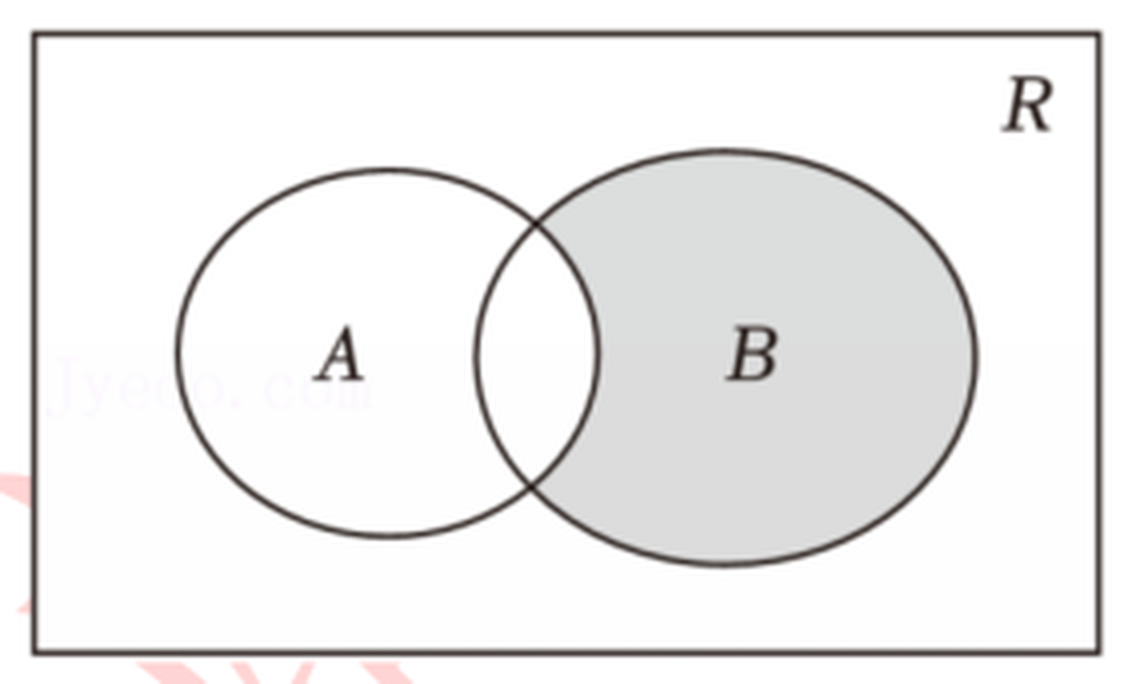
\includegraphics[width=0.30\textwidth]{figures/venn_Abar_cap_B.png}
\end{center}

\begin{enumerate}[label=(\arabic*)]
\item 若 $a=1$，求阴影部分表示的集合.
\item 若 $A\cap B=B$，求实数 $a$ 的取值范围.
\end{enumerate}

\ifanswer
\solbegin
\stepm{(1)}{因为 $\dfrac{2x-3}{x+5}\leqslant0$，
等价于 $\begin{cases}(2x-3)(x+5)\leqslant0\\ x+5\neq0\end{cases}$，}
\step{解得 $-5<x\leqslant\dfrac32$，即 $A=\left\{x\mid-5<x\leqslant\dfrac32\right\}$；}
\step{若 $a=1$，因为 $|x-1|<1$，等价于 $-1<x-1<1$，}
\step{解得 $0<x<2$，即 $B=\{x\mid0<x<2\}$.}
\step{由 Venn 图得阴影部分表示的集合为 $\overline{A}\cap B=\left(\dfrac32,2\right)$.}
\stepm{(2)}{由 (1) 得 $A=\left\{x\mid-5<x\leqslant\dfrac32\right\}$，}
\step{$B=\{x\mid|x-a|<1\}=\{x\mid-1+a<x<1+a\}\neq\varnothing$，}
\step{因为 $A\cap B=B$，所以 $B\sub A$，}
\step{所以 $\begin{cases}-5\leqslant-1+a\\ 1+a\leqslant\dfrac32\end{cases}$，
解得 $-4\leqslant a\leqslant\dfrac12$，}
\step{所以实数 $a$ 的取值范围为 $\left[-4,\dfrac12\right]$.}
\solend

\fi

\ansspace[6]

\item 设 $A=\{x\mid x^2-(m+3)x+2(m+1)=0,m\in\R\}$，
$B=\{x\mid 2x^2+(3n+1)x+2=0,n\in\R\}$.

\begin{enumerate}[label=(\arabic*)]
\item 是否存在 $m$、$n\in\R$，使得 $A=\{1,2\}$，$B=\varnothing$，说明理由；
\item 若 $A\cap B=A$，求 $m$、$n$ 的值.
\end{enumerate}

\ifanswer
\solbegin
\stepm{(1)}{由 $A=\{1,2\}$，得 $m=0$，}
\step{再由 $B=\varnothing$，得 $\Delta=(3n+1)^2-4\times2\times2=9n^2+6n-15<0$，}
\step{所以 $(3n+5)(n-1)<0$，解得 $-\dfrac53<n<1$，}
\step{故存在 $m=0$，$-\dfrac53<n<1$，使得 $A=\{1,2\}$，$B=\varnothing$.}
\stepm{(2)}{由 $x^2-(m+3)x+2(m+1)=0$，得 $x=2$ 或 $x=m+1$，}
\step{若 $A\cap B=A$，则 $A\sub B$，}
\step{将 $x=2$ 代入 $2x^2+(3n+1)x+2=0$，得 $n=-2$，}
\step{则 $B=\{x\mid 2x^2+(3n+1)x+2=0,n\in\R\}=\{x\mid 2x^2-5x+2=0\}
=\left\{2,\dfrac12\right\}$.}
\step{则 $m+1=\dfrac12$ 或 $m+1=2$，则 $m=-\dfrac12$ 或 $m=1$，
所以 $m=-\dfrac12$ 或 $m=1$，$n=-2$.}
\solend

\fi

\ansspace[6]

\item 已知陈述句 $\alpha$：关于 $x$ 的方程 $x^2-6x+m=0$ 有两个不同的正数根，陈述句
$\beta$：集合 $\{x\mid(m+1)x^2+4x+1=0,x\in\R\}$ 中至多有一个元素.

\begin{enumerate}[label=(\arabic*)]
\item 若 $\alpha$ 和 $\beta$ 都是真命题，求实数 $m$ 的取值范围；
\item 若 $\alpha$ 和 $\beta$ 至多有一个是假命题，求实数 $m$ 的取值范围.
\end{enumerate}

\ifanswer
\solbegin
\stepm{(1)}{因为关于 $x$ 的方程 $x^2-6x+m=0$ 有两个不同的正数根，}
\step{则 $\begin{cases}36-4m>0\\ m>0\end{cases}$，解得 $0<m<9$，}
\step{集合 $\{x\mid(m+1)x^2+4x+1=0,x\in\R\}$ 中至多有一个元素，}
\step{则 $m=-1$ 或 $\begin{cases}m+1\neq0\\ 16-4(m+1)\leqslant0\end{cases}$，
解得 $m\geqslant3$，}
\step{$\alpha$ 和 $\beta$ 都是真命题，所以实数 $m$ 的取值范围为 $\{m\mid3\leqslant m<9\}$}
\stepm{(2)}{由 (1) 得当 $\alpha$ 为假命题时，$m\leqslant0$ 或 $m\geqslant9$，}
\step{当 $\beta$ 为假命题时，$m<3$ 且 $m\neq-1$，}
\step{所以 $\alpha$ 和 $\beta$ 均为假命题时，$m$ 的范围是 $m\leqslant0$ 且 $m\neq-1$，}
\step{$\alpha$ 和 $\beta$ 至多有一个是假命题时，实数 $m$ 的取值范围为
$\{m\mid m>0$ 或 $m=-1\}$.}
\solend

\fi

\ansspace[6]

\item 已知符号 $[x]$ 表示不大于 $x$ 的最大整数 $(x\in\R)$，例如：$[1.3]=1$，
$[2]=2$，$[-1.2]=-2$.

\begin{enumerate}[label=(\arabic*)]
\item 已知方程 $[x]=3$，求该方程的解集；
\item 设方程 $\bigl[|x|+|x-1|\bigr]=3$ 的解集为 $A$，
集合 $B=\{x\mid 2x^2-11kx+15k^2\geqslant0\}$，若 $A\cup B=\R$，求实数 $k$ 的取值范围；
\item 在 (2) 的条件下，集合 $C=\{x\mid x^2-ax+1-2a\leqslant0,a\in\R\}$，是否存在实数
$a$，$A\cap C=A$，若存在，请求出实数 $a$ 的取值范围；若不存在，请说明理由.
\end{enumerate}

\ifanswer
\solbegin
\stepm{(1)}{方程 $[x]=3$，则 $x\in[3,4)$，所以该方程的解集为 $[3,4)$；}
\stepm{(2)}{因为 $\bigl[|x|+|x-1|\bigr]=3$，所以 $3\leqslant|x|+|x-1|<4$，}
\step{由绝对值不等式的几何意义得 $A=\left(-\dfrac32,-1\right]\cup\left[2,\dfrac52\right)$，}
\step{又 $B=\{x\mid 2x^2-11kx+15k^2\geqslant0\}=\{x\mid(2x-5k)(x-k)\geqslant0\}$，}
\step{当 $k=0$ 时，$B=\{x\mid 2x^2\geqslant0\}=\R$，则 $A\cup B=\R$，符合题意；}
\step{当 $k>0$ 时，$B=\left(-\infty,\dfrac{5k}{2}\right]\cup[3k,+\infty)$，
若 $A\cup B=\R$，}
\step{则 $\begin{cases}\dfrac{5k}{2}\geqslant2\\[2pt] 3k\leqslant\dfrac52\end{cases}$，
解得 $k\in\left[\dfrac45,\dfrac56\right]$；}
\step{当 $k<0$ 时，$B=(-\infty,3k]\cup\left[\dfrac{5k}{2},+\infty\right)$，
若 $A\cup B=\R$，}
\step{则 $\begin{cases}\dfrac{5k}{2}\leqslant-1\\[2pt] 3k\geqslant-\dfrac32\end{cases}$，
解得 $k\in\left[-\dfrac12,-\dfrac25\right]$.}
\step{综上所述，实数 $k$ 的取值范围为
$\left[-\dfrac12,-\dfrac25\right]\cup\{0\}\cup\left[\dfrac45,\dfrac56\right]$；}
\stepm{(3)}{因为 $A\cap C=A$，则 $A\sub C$ 且
$A=\left(-\dfrac32,-1\right]\cup\left[2,\dfrac52\right)$，}
\step{设集合 $C$ 的解集为 $(x_1,x_2)(x_1<x_2)$，}
\step{则 $\begin{cases}x_1\leqslant-\dfrac32\\[2pt] x_2\geqslant\dfrac52\end{cases}$，}
\step{所以
$\begin{cases}\Delta=a^2-4(1-2a)>0\\[2pt]
f\!\left(-\dfrac32\right)=\dfrac94+\dfrac32a+1-2a\leqslant0\\[4pt]
f\!\left(\dfrac52\right)=\dfrac{25}{4}-\dfrac52a+1-2a\leqslant0\end{cases}$，
解得 $a\geqslant\dfrac{13}{2}$，}
\step{故实数 $a$ 的取值范围为 $\left[\dfrac{13}{2},+\infty\right)$.}
\solend

\fi

\ansspace[6]

\item 非空有限集合 $S$ 是由若干个正实数组成，集合 $S$ 的元素个数不少于 $2$ 个. 对于任意
$a,b\in S,a\neq b$，若数 $a^b$ 或 $b^a$ 中至少有一个属于 $S$，则称集合 $S$ 是“好集”；
否则，称集合 $S$ 是“坏集”.

\begin{enumerate}[label=(\arabic*)]
\item 判断 $A=\{1,3,9\}$ 和 $B=\left\{1,\dfrac12,\dfrac14,\dfrac1{16}\right\}$ 是“好集”
还是“坏集”，并简单说明理由；
\item 题设的有限集 $S$ 中，既有大于 $1$ 的元素，又有小于 $1$ 的元素，证明：集合 $S$ 是
“坏集”；
\item 若题设中的 $a^b$ 或 $b^a$ 都属于 $S$，则称集合 $S$ 为“超级好集”，写出一个
“超级好集”（无须证明）.
\end{enumerate}

\ifanswer
\solbegin
\stepm{(1)}{$A=\{1,3,9\}$，$3^9\notin A$，$9^3\notin A$，所以 $A$ 是“坏集”，}
\step{从 $B$ 集合中任意取两个数字都满足需求，所以 $B$ 是“好集”.}
\stepm{(2)}{假设 $a$ 是 $S$ 中小于 $1$ 的元素中的最小元素，}
\step{$b$ 是 $S$ 中大于 $1$ 的元素中的最小元素，则 $a^b<a^1=a$，}
\step{所以 $a$ 就不是 $S$ 中小于 $1$ 的元素中的最小元素，即 $a^b\notin S$，}
\step{同理 $1=b^0<b^a<b^1=b$，所以 $b$ 就不是 $S$ 中大于 $1$ 的元素中的最小元素，}
\step{即 $b^a\notin S$，所以集合 $S$ 是“坏集”；}
\stepm{(3)}{首先 $S=\{1,a\}$（$a\neq1$ 且 $a>0$）是“超级好集”，}
\step{假设 $0<a<1$，由 (2) 得，$S$ 中不可能有大于 $1$ 的元素，}
\step{假设 $S$ 中有除 $a$ 之外的元素 $b\in S$（$a\neq b,b<1$），}
\step{假设 $a$ 是 $S$ 中小于 $1$ 的元素中的最大元素，$a^b>a^1=a$，}
\step{所以 $a$ 不是最大元素，所以 $a^b\notin S$，所以 $b\notin S$；}
\step{假设 $a>1$，由 (2) 得 $S$ 中不可能有小于 $1$ 的元素，}
\step{假设 $S$ 中有除 $a$ 之外的元素 $b$（$b>1$ 且 $b\neq a$），}
\step{假设 $a$ 是 $S$ 中大于 $1$ 的元素中的最小元素，则 $a^b>a^1=a$，}
\step{所以 $a$ 不是最小元素，即不存在 $b>1$，使得 $b\in S$，即 $b\notin S$，}
\step{综上，$S=\{1,a\}$（$a\neq1$ 且 $a>0$）.}
\solend

\fi

\ansspace*[10]

\end{enumerate}

\end{document}
"
% 紧凑版：xelatex "\def\iscompact{1}% 高一25_华师大二附中_周末作业3.tex
%   —— 高一上数学「2026-2027 年华师大二附中高一上周末作业 3」（试卷版/答案版）
% 试卷版：xelatex 高一25_华师大二附中_周末作业3.tex
% 答案版：xelatex "\def\isanswer{1}\input{高一25_华师大二附中_周末作业3.tex}"
% 紧凑版：xelatex "\def\iscompact{1}\input{高一25_华师大二附中_周末作业3.tex}"
%
% 原始材料是微信公众号图文（公众号「魔都数学加油站」连载「27学年高一 25」，2026-09-21 发布，
% 原文标题「27学年高一25——2026-2027年上海市华师大二附中高一上周末作业3」），
% 正文为 10 张 PNG 页（1080×1527，各页同尺寸）。原文本身就是一份**讲评版**——
% 题目下方直接印出【解析】（本卷无单独的【答案】行，填空题答案都写在解析里）。
% 试题文字与解析均照原卷录入，未改内容。卷面的粉色斜水印「魔都数学加油站」属水印，未录入。
%
% 卷首标题：原卷印作「2026-2027 年华师大二附中高一上周末作业 3」（公众号标题里的「上海市」
% 三字卷面标题行没有，本稿照卷面），年份区间按全稿惯例排 en dash，前缀照原卷保留「年」。
%
% 与原卷的排版差异（均已在 README「说明」中交代）：
%   ① 原文自**第 3 题**起（第 1、2 题未在该文中发布），故本稿题号亦自 3 起；
%   ② 原卷本就印有「一、填空题」「二、选择题」「三、解答题」三节标题，本稿照原卷分节，
%      只把标题改排成全稿统一的「大节标题」样式；
%   ③ 原卷第 13 题的答案「D」直接印在题干末尾的括号内，第 14—16 题的括号空着、答案写在
%      解析末句「故选 C／B」里；填空题的答案也都嵌在解析里，本稿统一改为试卷版隐去、
%      答案版以 \ans{} 给出（选择题另附【解析】），使两版彻底分离；
%   ④ 补集符号原卷一律作**上横线**（$\overline{A}$、$\overline{A\cup B}$），与同校的
%      高一14 同例，本稿照录（不改为 $\complement_U A$ 写法）；
%   ⑤ 原卷的实数集 R 斜体与粗体混用（第 17 题题干「全集为 R」作粗体，第 5、14 题与
%      第 16 题解析的 $R$ 为斜体），本稿按全稿惯例统一写作 $\R$；
%   ⑥ 原卷填空的横线约两个字宽，本稿按全稿惯例统一排 \blankline[4.4em]；
%   ⑦ 原卷未印副标题，本稿按全稿惯例补出副标题「集合与常用逻辑用语」；
%   ⑧ 第 17 题的 Venn 图原卷印在题干右侧（第 6 页），本稿移至题干之后；
%      图取原卷截图、4× LANCZOS 放大（figures/venn_Abar_cap_B.png，
%      阴影为 $B$ 中不含 $A\cap B$ 的部分，即 $\overline{A}\cap B$）。
%
% 原卷存疑两处（均照抄原卷、未改，见源码中该处上方注释）：
%   ① 第 8 题【解析】第二段「当 $\Delta=a^2-16>0$ 时，方程 $x^2+ax+4=0$ 有两个相同的根
%      $x_1$、$x_2$」——$\Delta>0$ 应为「两个**不**相同的根」（其自己的后文就把 $x_1$、$x_2$
%      当作可以不同的两个根在讨论），显系笔误；
%   ② 第 11 题【解析】先写「偶数必是 $2^{11}\cdot3^m\cdot337^n$，$m$、$n\in\N^*$」，
%      下一行又写「$0\leqslant m\leqslant10$，$0\leqslant n\leqslant10$，共有 121 种情况」
%      ——按 $\N^*$ 应从 1 起（至多 $10\times10=100$ 种），与 121（$=11\times11$，含 0）
%      对不上，两处至少有一处笔误。

\documentclass[a4paper,11pt]{article}
\usepackage{common}

\begin{document}

\examtitlest[3]{2026--2027 年华师大二附中高一上周末作业 3}{集合与常用逻辑用语}

\bigsec{一、填空题}

\begin{enumerate}
\setcounter{enumi}{2}

\item 设全集 $U=\{2,4,m^2+m-5\}$，集合 $A=\{2,1-m\}$，若 $\overline{A}=\{1\}$，则实数
$m=$ \blankline[4.4em].

\ifanswer
\solbegin
\step{因为 $\overline{A}=\{1\}$，所以 $1\in U$，$1\notin A$，}
\step{所以 $\begin{cases}m^2+m-5=1\\ 1-m\neq1\\ 1-m=4\end{cases}$，解得 $m=-3$.}
\solend

\fi

\item 已知条件 $\alpha$：$m<x\leqslant2m+5$，条件 $\beta$：$0\leqslant x\leqslant1$，
若 $\alpha$ 是 $\beta$ 的必要条件，则实数 $m$ 的取值范围为 \blankline[4.4em].

\ifanswer
\solbegin
\step{若 $\alpha$ 是 $\beta$ 的必要条件，则 $[0,1]\sub(m,2m+5]$，}
\step{所以 $\begin{cases}m<2m+5\\ m<0\\ 2m+5\geqslant1\end{cases}$，}
\step{解得 $-2\leqslant m<0$，故实数 $m$ 的取值范围为 $[-2,0)$.}
\solend

\fi

\item 已知 $\R$ 是全集，集合 $A=\{y\mid y=-x^2+1,x\in\R\}$，集合
$B=\{x\mid x=3+|a|,a\in\R\}$，则 $\overline{A\cup B}=$ \blankline[4.4em].

\ifanswer
\solbegin
\step{$A=\{y\mid y=-x^2+1,x\in\R\}=(-\infty,1]$，}
\step{$B=\{x\mid x=3+|a|,a\in\R\}=[3,+\infty)$，}
\step{所以 $\overline{A\cup B}=(1,3)$.}
\solend

\fi

\item 已知 $a$ 为常数，集合 $A=\{x\mid x^2+x-6=0\}$，集合 $B=\{x\mid ax-2=0\}$，且
$B\sub A$，则 $a$ 的所有取值构成的集合为 \blankline[4.4em].

\ifanswer
\solbegin
\step{集合 $A=\{-3,2\}$，因为 $B\sub A$，所以 $B=\varnothing$，$\{-3\}$，$\{2\}$，$\{-3,2\}$，}
\step{当 $B=\varnothing$ 时，$a=0$，当 $B=\{-3\}$ 时，$a=-\dfrac23$，当 $B=\{2\}$ 时，$a=1$，}
\step{当 $B=\{-3,2\}$ 时，不成立，故 $a$ 的取值集合为 $\left\{0,-\dfrac23,1\right\}$.}
\solend

\fi

\item 已知一元二次方程 $x^2+px+p=0$ 有两个不相等的实根分别为 $x_1$、$x_2$.
$A=x_1^2+x_2^2$，$B=x_1x_2(x_1+x_2)$，$A$ 与 $B$ 的大小为 \blankline[4.4em].

\ifanswer
\solbegin
\step{一元二次方程 $x^2+px+p=0$ 有两个不相等的实根分别为 $x_1$、$x_2$，}
\step{则 $\Delta=p^2-4p>0$，解得 $p<0$ 或 $p>4$，}
\step{由韦达定理得 $x_1+x_2=-p$，$x_1x_2=p$，}
\step{所以 $A=x_1^2+x_2^2=(x_1+x_2)^2-2x_1x_2=p^2-2p$，$B=x_1x_2(x_1+x_2)=-p^2$，}
\step{所以 $A-B=(p^2-2p)-(-p^2)=2p(p-1)$，}
\step{当 $p<0$ 时，则 $A-B>0$，故 $A>B$，}
\step{当 $p>4$ 时，则 $A-B>0$，故 $A>B$，}
\step{综上，$A=p^2-2p$，$B=-p^2$，且 $A>B$.}
\solend

\fi

\item 集合 $A=\{x\mid(x-1)(x^2+ax+4)=0,x\in\R\}$ 中所有元素之和为 $3$，则实数
$a=$ \blankline[4.4em].

\ifanswer
\solbegin
\step{当 $\Delta=a^2-16=0$ 时，方程 $x^2+ax+4=0$ 有两个相同的根 $-\dfrac a2$，}
\step{则 $A=\left\{1,-\dfrac a2\right\}$，故 $1-\dfrac a2=3$，解得 $a=-4$；}
% 注：下一行的「两个相同的根」系原卷笔误（△>0 应为「两个不相同的根」，其自己的后文
%     就把 x₁、x₂ 当作可以不同的两个根在讨论），照抄原卷、未改，见文件头「原卷存疑」①。
\step{当 $\Delta=a^2-16>0$ 时，方程 $x^2+ax+4=0$ 有两个相同的根 $x_1$、$x_2$，}
\step{若 $1$ 是方程 $x^2+ax+4=0$ 的根，则方程 $x^2+ax+4=0$ 的另一个根为 $4$，}
\step{则 $A=\{1,4\}$，不成立；}
\step{若 $1$ 不是方程 $x^2+ax+4=0$ 的根，则 $A=\{1,x_1,x_2\}$，则 $1+x_1+x_2=3$，}
\step{故 $x_1+x_2=2=-a$，故 $a=-2$（舍去）；}
\step{综上所述，$a=-4$.}
\solend

\fi

\item 已知集合 $A=\{x\mid x^2+2x-8\geqslant0\}$，$B=\{x\mid x^2-2ax+4\leqslant0\}$，
若 $a>0$，且 $A\cap B\cap\N$ 中恰有 $2$ 个元素，则 $a$ 的取值范围为 \blankline[4.4em].

\ifanswer
\solbegin
\step{由 $A$ 中不等式变形得 $(x-2)(x+4)\geqslant0$，解得 $x\leqslant-4$ 或 $x\geqslant2$，}
\step{即 $A=(-\infty,-4]\cup[2,+\infty)$，}
\step{设 $f(x)=x^2-2ax+4$，则 $f(x)$ 的轴对称 $x=a>0$，}
\step{且对应方程的根 $x_1$、$x_2$ 满足 $\begin{cases}x_1x_2=4\\ x_1+x_2>0\end{cases}$，}
\step{所以 $0<x_1\leqslant2\leqslant x_2$（取 $x_1\leqslant x_2$），}
\step{所以 $A\cap B\cap\N$ 中恰有的整数为 $2$，$3$，}
\step{所以 $\begin{cases}f(3)=9-6a+4\leqslant0\\ f(4)=16-8a+4>0\end{cases}$，}
\step{解得 $\dfrac{13}{6}\leqslant a<\dfrac52$，所以 $a$ 的取值范围为 $\left[\dfrac{13}{6},\dfrac52\right)$.}
\solend

\fi

\item 在三个关于 $x$ 的方程 $x^2-ax+4=0$，$x^2+(a-1)x+16=0$ 和
$x^2+2ax+3a+10=0$ 中至少有一个方程有实根，则实数 $a$ 的取值范围是 \blankline[4.4em].

\ifanswer
\solbegin
\step{当三个方程均无实根时，有}
\step{$\begin{cases}\Delta_1=a^2-16<0\\ \Delta_2=(a-1)^2-64<0\\ \Delta_3=4a^2-4(3a+10)<0\end{cases}$，}
\step{所以 $\begin{cases}-4<a<4\\ -7<a<9\\ -2<a<5\end{cases}$，}
\step{所以 $-2<a<4$，故三个方程均无实根时，$a$ 的取值范围为 $(-2,4)$，}
\step{所以三个方程中至少有一个方程有实根时，}
\step{实数 $a$ 的取值范围为 $(-\infty,-2]\cup[4,+\infty)$.}
\solend

\fi

% 注：下一行解析里的「m、n∈N*」与再下一行的「0≤m≤10，0≤n≤10，共有 121 种情况」
%     对不上（按 N* 应从 1 起，至多 10×10=100 种；121=11×11 含 0），系原卷自身矛盾，
%     照抄原卷、未改，见文件头「原卷存疑」②。
\item 若集合 $M=\{(x,y)\mid(x+1)+(x+2)+\cdots+(x+y)=2022^{10},x\in\Z,y\in\N^{*}\}$，
则集合 $M$ 中元素有 \blankline[4.4em] 个.

\ifanswer
\solbegin
\step{由题意得 $(x+1)+(x+2)+\cdots+(x+y)=\dfrac{y(2x+1+y)}{2}$，}
\step{所以 $y(2x+1+y)=2^{11}\cdot3^{10}\cdot337^{10}$，}
\step{因为 $y$ 与 $2x+1+y$ 必为一奇一偶，偶数必是 $2^{11}\cdot3^m\cdot337^n$，
$m$、$n\in\N^{*}$，}
\step{$0\leqslant m\leqslant10$，$0\leqslant n\leqslant10$，共有 $121$ 种情况，}
\step{因为 $y$ 与 $2x+1+y$ 奇偶未定，所以集合 $M$ 中元素只有 $242$ 个.}
\solend

\fi

\item 设集合 $M=\left\{x\mid m\leqslant x\leqslant m+\dfrac34\right\}$，
$N=\left\{x\mid n-\dfrac13\leqslant x\leqslant n\right\}$，且 $M$、$N$ 都是集合
$\{x\mid0\leqslant x\leqslant1\}$ 的子集，如果把 $b-a$ 叫做集合
$\{x\mid a\leqslant x\leqslant b\}$ 的长度，那么集合 $M\cap N$ 的长度的最小值是
\blankline[4.4em].

\ifanswer
\solbegin
\step{$M$ 的长度为 $\dfrac34$，$N$ 的长度为 $\dfrac13$，}
\step{当集合 $M\cap N$ 的长度的最小值时，$M$ 与 $N$ 应分别在区间 $[0,1]$ 的左右两端，}
\step{故 $M\cap N$ 的长度的最小值是 $\dfrac34+\dfrac13-1=\dfrac1{12}$.}
\solend

\fi

\end{enumerate}

\bigsec{二、选择题}

\begin{enumerate}
\setcounter{enumi}{12}

\item 直角坐标平面中除去两点 $A(1,1)$、$B(2,-2)$ 可用集合表示为\mbox{（\quad）}

\keepwithprev
A. $\{(x,y)\mid x\neq1,y\neq1,x\neq2,y\neq-2$\}\qquad
B. $\{(x,y)\mid\begin{cases}x\neq1\\ y\neq1\end{cases}$ 或 $\begin{cases}x\neq2\\ y\neq-2\end{cases}\}$

C. $\{(x,y)\mid[(x-1)^2+(y-1)^2][(x-2)^2+(y+2)^2]\neq0$\}

D. $\{(x,y)\mid[(x-1)^2+(y-1)^2]+[(x-2)^2+(y+2)^2]\neq0$\}

\ans{$D$}

\item 已知函数 $f(x)=x^2+nx$，记集合 $A=\{x\mid f(x)=0,x\in\R\}$，
$B=\{x\mid f(f(x))=0,x\in\R\}$，若 $A=B\neq\varnothing$，则 $n$ 的取值范围是\mbox{（\quad）}

\keepwithprev
A. $[0,4]$\qquad B. $(0,4)$\qquad C. $[0,4)$\qquad D. $(0,4]$

\ans{$C$}

\ifanswer
\solbegin
\step{$f(x)=x^2+nx$，$f[f(x)]=(x^2+nx)^2+n(x^2+nx)=(x^2+nx)(x^2+nx+n)$，}
\step{当 $n=0$ 时，$f(x)=x^2$，$f[f(x)]=x^4$，满足 $A=B$，此时 $n=0$；}
\step{当 $n\neq0$ 时，$0$、$-n$ 不是 $x^2+nx+n=0$ 的根，故 $\Delta=n^2-4n<0$，
解得 $0<n<4$，}
\step{综上所述，$n$ 的取值范围是 $[0,4)$. 故选 $C$.}
\solend

\fi

\item 设全集 $U=\{1,2,3,4,5,6,7,8,9,10\}$，给出条件：① $A\sub U$；②若 $x\in A$，
则 $2x\notin A$；③若 $x\in\overline{A}$，则 $2x\notin\overline{A}$.
那么同时满足三个条件的集合 $A$ 的个数为\mbox{（\quad）}

\keepwithprev
A. $0$ 个\qquad B. $16$ 个\qquad C. $32$ 个\qquad D. $64$ 个

\ans{$C$}

\ifanswer
\solbegin
\step{由① $A\sub U$；②若 $x\in A$，则 $2x\notin A$；③若 $x\in\overline{A}$，
则 $2x\notin\overline{A}$.}
\step{若 $1\in A$，则 $2\notin A$，即 $2\in\overline{A}$，则 $4\notin\overline{A}$，
即 $4\in A$，则 $8\notin A$，即 $8\in\overline{A}$；}
\step{若 $3\in A$，则 $6\notin A$，即 $6\in\overline{A}$；若 $5\in A$，则 $10\notin A$，
即 $10\in\overline{A}$，}
\step{故 $1$、$4$ 和 $2$、$8$ 分开，$3$ 和 $6$ 分开，$5$ 和 $10$ 分开，$7$ 和 $9$ 随意，}
\step{故同时满足三个条件的集合 $A$ 的个数为 $2\times2\times2\times2\times2=32$，
故选 $C$.}
\solend

\fi

\item 设集合 $P_1=\{x\mid x^2+ax+1>0\}$，$P_2=\{x\mid x^2+ax+2>0\}$，
$Q_1=\{x\mid x^2+x+b>0\}$，$Q_2=\{x\mid x^2+2x+b>0\}$，其中 $a$、$b\in\R$，
下列说法中正确的是\mbox{（\quad）}

\keepwithprev
A. 对任意 $a$，$P_1$ 是 $P_2$ 的子集，对任意的 $b$，$Q_1$ 不是 $Q_2$ 的子集

B. 对任意 $a$，$P_1$ 是 $P_2$ 的子集，存在 $b$，使得 $Q_1$ 是 $Q_2$ 的子集

C. 存在 $a$，使得 $P_1$ 不是 $P_2$ 的子集，对任意的 $b$，$Q_1$ 不是 $Q_2$ 的子集

D. 存在 $a$，使得 $P_1$ 不是 $P_2$ 的子集，存在 $b$，使得 $Q_1$ 是 $Q_2$ 的子集

\ans{$B$}

\ifanswer
\solbegin
\step{对于集合 $P_1=\{x\mid x^2+ax+1>0\}$，$P_2=\{x\mid x^2+ax+2>0\}$，}
\step{得当 $m\in P_1$ 时，即 $m^2+am+1>0$，得 $m^2+am+2>0$，}
\step{即有 $m\in P_2$，得对任意 $a$，$P_1$ 是 $P_2$ 的子集，}
\step{对于集合 $Q_1=\{x\mid x^2+x+b>0\}$，$Q_2=\{x\mid x^2+2x+b>0\}$，}
\step{当 $b=6$ 时，$Q_1=\{x\mid x^2+x+6>0\}=\R$，$Q_2=\{x\mid x^2+2x+6>0\}=\R$，}
\step{得 $Q_1$ 是 $Q_2$ 的子集，}
\step{当 $b=1$ 时，$Q_1=\{x\mid x^2+x+1>0\}=\R$，}
\step{$Q_2=\{x\mid x^2+2x+1>0\}=\{x\mid x\neq-1\}$，得 $Q_1$ 不是 $Q_2$ 的子集，}
\step{所以存在 $b$，使得 $Q_1$ 是 $Q_2$ 的子集，故选 $B$.}
\solend

\fi

\end{enumerate}

\bigsec{三、解答题}

\begin{enumerate}
\setcounter{enumi}{16}

\item 已知集合 $A=\left\{x\mid\dfrac{2x-3}{x+5}\leqslant0\right\}$，
$B=\{x\mid|x-a|<1\}$，全集为 $\R$.

\begin{center}
% 图取原卷截图、4× LANCZOS 放大（原卷把图印在题干右侧，本稿移至此处，见文件头⑧）。
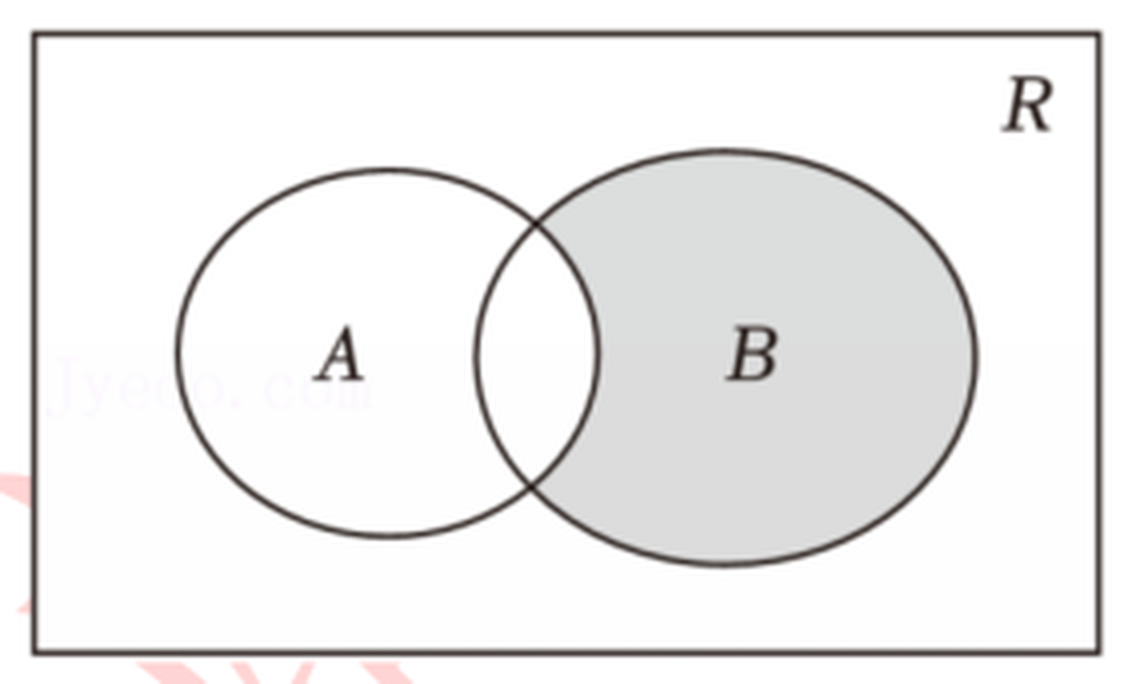
\includegraphics[width=0.30\textwidth]{figures/venn_Abar_cap_B.png}
\end{center}

\begin{enumerate}[label=(\arabic*)]
\item 若 $a=1$，求阴影部分表示的集合.
\item 若 $A\cap B=B$，求实数 $a$ 的取值范围.
\end{enumerate}

\ifanswer
\solbegin
\stepm{(1)}{因为 $\dfrac{2x-3}{x+5}\leqslant0$，
等价于 $\begin{cases}(2x-3)(x+5)\leqslant0\\ x+5\neq0\end{cases}$，}
\step{解得 $-5<x\leqslant\dfrac32$，即 $A=\left\{x\mid-5<x\leqslant\dfrac32\right\}$；}
\step{若 $a=1$，因为 $|x-1|<1$，等价于 $-1<x-1<1$，}
\step{解得 $0<x<2$，即 $B=\{x\mid0<x<2\}$.}
\step{由 Venn 图得阴影部分表示的集合为 $\overline{A}\cap B=\left(\dfrac32,2\right)$.}
\stepm{(2)}{由 (1) 得 $A=\left\{x\mid-5<x\leqslant\dfrac32\right\}$，}
\step{$B=\{x\mid|x-a|<1\}=\{x\mid-1+a<x<1+a\}\neq\varnothing$，}
\step{因为 $A\cap B=B$，所以 $B\sub A$，}
\step{所以 $\begin{cases}-5\leqslant-1+a\\ 1+a\leqslant\dfrac32\end{cases}$，
解得 $-4\leqslant a\leqslant\dfrac12$，}
\step{所以实数 $a$ 的取值范围为 $\left[-4,\dfrac12\right]$.}
\solend

\fi

\ansspace[6]

\item 设 $A=\{x\mid x^2-(m+3)x+2(m+1)=0,m\in\R\}$，
$B=\{x\mid 2x^2+(3n+1)x+2=0,n\in\R\}$.

\begin{enumerate}[label=(\arabic*)]
\item 是否存在 $m$、$n\in\R$，使得 $A=\{1,2\}$，$B=\varnothing$，说明理由；
\item 若 $A\cap B=A$，求 $m$、$n$ 的值.
\end{enumerate}

\ifanswer
\solbegin
\stepm{(1)}{由 $A=\{1,2\}$，得 $m=0$，}
\step{再由 $B=\varnothing$，得 $\Delta=(3n+1)^2-4\times2\times2=9n^2+6n-15<0$，}
\step{所以 $(3n+5)(n-1)<0$，解得 $-\dfrac53<n<1$，}
\step{故存在 $m=0$，$-\dfrac53<n<1$，使得 $A=\{1,2\}$，$B=\varnothing$.}
\stepm{(2)}{由 $x^2-(m+3)x+2(m+1)=0$，得 $x=2$ 或 $x=m+1$，}
\step{若 $A\cap B=A$，则 $A\sub B$，}
\step{将 $x=2$ 代入 $2x^2+(3n+1)x+2=0$，得 $n=-2$，}
\step{则 $B=\{x\mid 2x^2+(3n+1)x+2=0,n\in\R\}=\{x\mid 2x^2-5x+2=0\}
=\left\{2,\dfrac12\right\}$.}
\step{则 $m+1=\dfrac12$ 或 $m+1=2$，则 $m=-\dfrac12$ 或 $m=1$，
所以 $m=-\dfrac12$ 或 $m=1$，$n=-2$.}
\solend

\fi

\ansspace[6]

\item 已知陈述句 $\alpha$：关于 $x$ 的方程 $x^2-6x+m=0$ 有两个不同的正数根，陈述句
$\beta$：集合 $\{x\mid(m+1)x^2+4x+1=0,x\in\R\}$ 中至多有一个元素.

\begin{enumerate}[label=(\arabic*)]
\item 若 $\alpha$ 和 $\beta$ 都是真命题，求实数 $m$ 的取值范围；
\item 若 $\alpha$ 和 $\beta$ 至多有一个是假命题，求实数 $m$ 的取值范围.
\end{enumerate}

\ifanswer
\solbegin
\stepm{(1)}{因为关于 $x$ 的方程 $x^2-6x+m=0$ 有两个不同的正数根，}
\step{则 $\begin{cases}36-4m>0\\ m>0\end{cases}$，解得 $0<m<9$，}
\step{集合 $\{x\mid(m+1)x^2+4x+1=0,x\in\R\}$ 中至多有一个元素，}
\step{则 $m=-1$ 或 $\begin{cases}m+1\neq0\\ 16-4(m+1)\leqslant0\end{cases}$，
解得 $m\geqslant3$，}
\step{$\alpha$ 和 $\beta$ 都是真命题，所以实数 $m$ 的取值范围为 $\{m\mid3\leqslant m<9\}$}
\stepm{(2)}{由 (1) 得当 $\alpha$ 为假命题时，$m\leqslant0$ 或 $m\geqslant9$，}
\step{当 $\beta$ 为假命题时，$m<3$ 且 $m\neq-1$，}
\step{所以 $\alpha$ 和 $\beta$ 均为假命题时，$m$ 的范围是 $m\leqslant0$ 且 $m\neq-1$，}
\step{$\alpha$ 和 $\beta$ 至多有一个是假命题时，实数 $m$ 的取值范围为
$\{m\mid m>0$ 或 $m=-1\}$.}
\solend

\fi

\ansspace[6]

\item 已知符号 $[x]$ 表示不大于 $x$ 的最大整数 $(x\in\R)$，例如：$[1.3]=1$，
$[2]=2$，$[-1.2]=-2$.

\begin{enumerate}[label=(\arabic*)]
\item 已知方程 $[x]=3$，求该方程的解集；
\item 设方程 $\bigl[|x|+|x-1|\bigr]=3$ 的解集为 $A$，
集合 $B=\{x\mid 2x^2-11kx+15k^2\geqslant0\}$，若 $A\cup B=\R$，求实数 $k$ 的取值范围；
\item 在 (2) 的条件下，集合 $C=\{x\mid x^2-ax+1-2a\leqslant0,a\in\R\}$，是否存在实数
$a$，$A\cap C=A$，若存在，请求出实数 $a$ 的取值范围；若不存在，请说明理由.
\end{enumerate}

\ifanswer
\solbegin
\stepm{(1)}{方程 $[x]=3$，则 $x\in[3,4)$，所以该方程的解集为 $[3,4)$；}
\stepm{(2)}{因为 $\bigl[|x|+|x-1|\bigr]=3$，所以 $3\leqslant|x|+|x-1|<4$，}
\step{由绝对值不等式的几何意义得 $A=\left(-\dfrac32,-1\right]\cup\left[2,\dfrac52\right)$，}
\step{又 $B=\{x\mid 2x^2-11kx+15k^2\geqslant0\}=\{x\mid(2x-5k)(x-k)\geqslant0\}$，}
\step{当 $k=0$ 时，$B=\{x\mid 2x^2\geqslant0\}=\R$，则 $A\cup B=\R$，符合题意；}
\step{当 $k>0$ 时，$B=\left(-\infty,\dfrac{5k}{2}\right]\cup[3k,+\infty)$，
若 $A\cup B=\R$，}
\step{则 $\begin{cases}\dfrac{5k}{2}\geqslant2\\[2pt] 3k\leqslant\dfrac52\end{cases}$，
解得 $k\in\left[\dfrac45,\dfrac56\right]$；}
\step{当 $k<0$ 时，$B=(-\infty,3k]\cup\left[\dfrac{5k}{2},+\infty\right)$，
若 $A\cup B=\R$，}
\step{则 $\begin{cases}\dfrac{5k}{2}\leqslant-1\\[2pt] 3k\geqslant-\dfrac32\end{cases}$，
解得 $k\in\left[-\dfrac12,-\dfrac25\right]$.}
\step{综上所述，实数 $k$ 的取值范围为
$\left[-\dfrac12,-\dfrac25\right]\cup\{0\}\cup\left[\dfrac45,\dfrac56\right]$；}
\stepm{(3)}{因为 $A\cap C=A$，则 $A\sub C$ 且
$A=\left(-\dfrac32,-1\right]\cup\left[2,\dfrac52\right)$，}
\step{设集合 $C$ 的解集为 $(x_1,x_2)(x_1<x_2)$，}
\step{则 $\begin{cases}x_1\leqslant-\dfrac32\\[2pt] x_2\geqslant\dfrac52\end{cases}$，}
\step{所以
$\begin{cases}\Delta=a^2-4(1-2a)>0\\[2pt]
f\!\left(-\dfrac32\right)=\dfrac94+\dfrac32a+1-2a\leqslant0\\[4pt]
f\!\left(\dfrac52\right)=\dfrac{25}{4}-\dfrac52a+1-2a\leqslant0\end{cases}$，
解得 $a\geqslant\dfrac{13}{2}$，}
\step{故实数 $a$ 的取值范围为 $\left[\dfrac{13}{2},+\infty\right)$.}
\solend

\fi

\ansspace[6]

\item 非空有限集合 $S$ 是由若干个正实数组成，集合 $S$ 的元素个数不少于 $2$ 个. 对于任意
$a,b\in S,a\neq b$，若数 $a^b$ 或 $b^a$ 中至少有一个属于 $S$，则称集合 $S$ 是“好集”；
否则，称集合 $S$ 是“坏集”.

\begin{enumerate}[label=(\arabic*)]
\item 判断 $A=\{1,3,9\}$ 和 $B=\left\{1,\dfrac12,\dfrac14,\dfrac1{16}\right\}$ 是“好集”
还是“坏集”，并简单说明理由；
\item 题设的有限集 $S$ 中，既有大于 $1$ 的元素，又有小于 $1$ 的元素，证明：集合 $S$ 是
“坏集”；
\item 若题设中的 $a^b$ 或 $b^a$ 都属于 $S$，则称集合 $S$ 为“超级好集”，写出一个
“超级好集”（无须证明）.
\end{enumerate}

\ifanswer
\solbegin
\stepm{(1)}{$A=\{1,3,9\}$，$3^9\notin A$，$9^3\notin A$，所以 $A$ 是“坏集”，}
\step{从 $B$ 集合中任意取两个数字都满足需求，所以 $B$ 是“好集”.}
\stepm{(2)}{假设 $a$ 是 $S$ 中小于 $1$ 的元素中的最小元素，}
\step{$b$ 是 $S$ 中大于 $1$ 的元素中的最小元素，则 $a^b<a^1=a$，}
\step{所以 $a$ 就不是 $S$ 中小于 $1$ 的元素中的最小元素，即 $a^b\notin S$，}
\step{同理 $1=b^0<b^a<b^1=b$，所以 $b$ 就不是 $S$ 中大于 $1$ 的元素中的最小元素，}
\step{即 $b^a\notin S$，所以集合 $S$ 是“坏集”；}
\stepm{(3)}{首先 $S=\{1,a\}$（$a\neq1$ 且 $a>0$）是“超级好集”，}
\step{假设 $0<a<1$，由 (2) 得，$S$ 中不可能有大于 $1$ 的元素，}
\step{假设 $S$ 中有除 $a$ 之外的元素 $b\in S$（$a\neq b,b<1$），}
\step{假设 $a$ 是 $S$ 中小于 $1$ 的元素中的最大元素，$a^b>a^1=a$，}
\step{所以 $a$ 不是最大元素，所以 $a^b\notin S$，所以 $b\notin S$；}
\step{假设 $a>1$，由 (2) 得 $S$ 中不可能有小于 $1$ 的元素，}
\step{假设 $S$ 中有除 $a$ 之外的元素 $b$（$b>1$ 且 $b\neq a$），}
\step{假设 $a$ 是 $S$ 中大于 $1$ 的元素中的最小元素，则 $a^b>a^1=a$，}
\step{所以 $a$ 不是最小元素，即不存在 $b>1$，使得 $b\in S$，即 $b\notin S$，}
\step{综上，$S=\{1,a\}$（$a\neq1$ 且 $a>0$）.}
\solend

\fi

\ansspace*[10]

\end{enumerate}

\end{document}
"
%
% 原始材料是微信公众号图文（公众号「魔都数学加油站」连载「27学年高一 25」，2026-09-21 发布，
% 原文标题「27学年高一25——2026-2027年上海市华师大二附中高一上周末作业3」），
% 正文为 10 张 PNG 页（1080×1527，各页同尺寸）。原文本身就是一份**讲评版**——
% 题目下方直接印出【解析】（本卷无单独的【答案】行，填空题答案都写在解析里）。
% 试题文字与解析均照原卷录入，未改内容。卷面的粉色斜水印「魔都数学加油站」属水印，未录入。
%
% 卷首标题：原卷印作「2026-2027 年华师大二附中高一上周末作业 3」（公众号标题里的「上海市」
% 三字卷面标题行没有，本稿照卷面），年份区间按全稿惯例排 en dash，前缀照原卷保留「年」。
%
% 与原卷的排版差异（均已在 README「说明」中交代）：
%   ① 原文自**第 3 题**起（第 1、2 题未在该文中发布），故本稿题号亦自 3 起；
%   ② 原卷本就印有「一、填空题」「二、选择题」「三、解答题」三节标题，本稿照原卷分节，
%      只把标题改排成全稿统一的「大节标题」样式；
%   ③ 原卷第 13 题的答案「D」直接印在题干末尾的括号内，第 14—16 题的括号空着、答案写在
%      解析末句「故选 C／B」里；填空题的答案也都嵌在解析里，本稿统一改为试卷版隐去、
%      答案版以 \ans{} 给出（选择题另附【解析】），使两版彻底分离；
%   ④ 补集符号原卷一律作**上横线**（$\overline{A}$、$\overline{A\cup B}$），与同校的
%      高一14 同例，本稿照录（不改为 $\complement_U A$ 写法）；
%   ⑤ 原卷的实数集 R 斜体与粗体混用（第 17 题题干「全集为 R」作粗体，第 5、14 题与
%      第 16 题解析的 $R$ 为斜体），本稿按全稿惯例统一写作 $\R$；
%   ⑥ 原卷填空的横线约两个字宽，本稿按全稿惯例统一排 \blankline[4.4em]；
%   ⑦ 原卷未印副标题，本稿按全稿惯例补出副标题「集合与常用逻辑用语」；
%   ⑧ 第 17 题的 Venn 图原卷印在题干右侧（第 6 页），本稿移至题干之后；
%      图取原卷截图、4× LANCZOS 放大（figures/venn_Abar_cap_B.png，
%      阴影为 $B$ 中不含 $A\cap B$ 的部分，即 $\overline{A}\cap B$）。
%
% 原卷存疑两处（均照抄原卷、未改，见源码中该处上方注释）：
%   ① 第 8 题【解析】第二段「当 $\Delta=a^2-16>0$ 时，方程 $x^2+ax+4=0$ 有两个相同的根
%      $x_1$、$x_2$」——$\Delta>0$ 应为「两个**不**相同的根」（其自己的后文就把 $x_1$、$x_2$
%      当作可以不同的两个根在讨论），显系笔误；
%   ② 第 11 题【解析】先写「偶数必是 $2^{11}\cdot3^m\cdot337^n$，$m$、$n\in\N^*$」，
%      下一行又写「$0\leqslant m\leqslant10$，$0\leqslant n\leqslant10$，共有 121 种情况」
%      ——按 $\N^*$ 应从 1 起（至多 $10\times10=100$ 种），与 121（$=11\times11$，含 0）
%      对不上，两处至少有一处笔误。

\documentclass[a4paper,11pt]{article}
\usepackage{common}

\begin{document}

\examtitlest[3]{2026--2027 年华师大二附中高一上周末作业 3}{集合与常用逻辑用语}

\bigsec{一、填空题}

\begin{enumerate}
\setcounter{enumi}{2}

\item 设全集 $U=\{2,4,m^2+m-5\}$，集合 $A=\{2,1-m\}$，若 $\overline{A}=\{1\}$，则实数
$m=$ \blankline[4.4em].

\ifanswer
\solbegin
\step{因为 $\overline{A}=\{1\}$，所以 $1\in U$，$1\notin A$，}
\step{所以 $\begin{cases}m^2+m-5=1\\ 1-m\neq1\\ 1-m=4\end{cases}$，解得 $m=-3$.}
\solend

\fi

\item 已知条件 $\alpha$：$m<x\leqslant2m+5$，条件 $\beta$：$0\leqslant x\leqslant1$，
若 $\alpha$ 是 $\beta$ 的必要条件，则实数 $m$ 的取值范围为 \blankline[4.4em].

\ifanswer
\solbegin
\step{若 $\alpha$ 是 $\beta$ 的必要条件，则 $[0,1]\sub(m,2m+5]$，}
\step{所以 $\begin{cases}m<2m+5\\ m<0\\ 2m+5\geqslant1\end{cases}$，}
\step{解得 $-2\leqslant m<0$，故实数 $m$ 的取值范围为 $[-2,0)$.}
\solend

\fi

\item 已知 $\R$ 是全集，集合 $A=\{y\mid y=-x^2+1,x\in\R\}$，集合
$B=\{x\mid x=3+|a|,a\in\R\}$，则 $\overline{A\cup B}=$ \blankline[4.4em].

\ifanswer
\solbegin
\step{$A=\{y\mid y=-x^2+1,x\in\R\}=(-\infty,1]$，}
\step{$B=\{x\mid x=3+|a|,a\in\R\}=[3,+\infty)$，}
\step{所以 $\overline{A\cup B}=(1,3)$.}
\solend

\fi

\item 已知 $a$ 为常数，集合 $A=\{x\mid x^2+x-6=0\}$，集合 $B=\{x\mid ax-2=0\}$，且
$B\sub A$，则 $a$ 的所有取值构成的集合为 \blankline[4.4em].

\ifanswer
\solbegin
\step{集合 $A=\{-3,2\}$，因为 $B\sub A$，所以 $B=\varnothing$，$\{-3\}$，$\{2\}$，$\{-3,2\}$，}
\step{当 $B=\varnothing$ 时，$a=0$，当 $B=\{-3\}$ 时，$a=-\dfrac23$，当 $B=\{2\}$ 时，$a=1$，}
\step{当 $B=\{-3,2\}$ 时，不成立，故 $a$ 的取值集合为 $\left\{0,-\dfrac23,1\right\}$.}
\solend

\fi

\item 已知一元二次方程 $x^2+px+p=0$ 有两个不相等的实根分别为 $x_1$、$x_2$.
$A=x_1^2+x_2^2$，$B=x_1x_2(x_1+x_2)$，$A$ 与 $B$ 的大小为 \blankline[4.4em].

\ifanswer
\solbegin
\step{一元二次方程 $x^2+px+p=0$ 有两个不相等的实根分别为 $x_1$、$x_2$，}
\step{则 $\Delta=p^2-4p>0$，解得 $p<0$ 或 $p>4$，}
\step{由韦达定理得 $x_1+x_2=-p$，$x_1x_2=p$，}
\step{所以 $A=x_1^2+x_2^2=(x_1+x_2)^2-2x_1x_2=p^2-2p$，$B=x_1x_2(x_1+x_2)=-p^2$，}
\step{所以 $A-B=(p^2-2p)-(-p^2)=2p(p-1)$，}
\step{当 $p<0$ 时，则 $A-B>0$，故 $A>B$，}
\step{当 $p>4$ 时，则 $A-B>0$，故 $A>B$，}
\step{综上，$A=p^2-2p$，$B=-p^2$，且 $A>B$.}
\solend

\fi

\item 集合 $A=\{x\mid(x-1)(x^2+ax+4)=0,x\in\R\}$ 中所有元素之和为 $3$，则实数
$a=$ \blankline[4.4em].

\ifanswer
\solbegin
\step{当 $\Delta=a^2-16=0$ 时，方程 $x^2+ax+4=0$ 有两个相同的根 $-\dfrac a2$，}
\step{则 $A=\left\{1,-\dfrac a2\right\}$，故 $1-\dfrac a2=3$，解得 $a=-4$；}
% 注：下一行的「两个相同的根」系原卷笔误（△>0 应为「两个不相同的根」，其自己的后文
%     就把 x₁、x₂ 当作可以不同的两个根在讨论），照抄原卷、未改，见文件头「原卷存疑」①。
\step{当 $\Delta=a^2-16>0$ 时，方程 $x^2+ax+4=0$ 有两个相同的根 $x_1$、$x_2$，}
\step{若 $1$ 是方程 $x^2+ax+4=0$ 的根，则方程 $x^2+ax+4=0$ 的另一个根为 $4$，}
\step{则 $A=\{1,4\}$，不成立；}
\step{若 $1$ 不是方程 $x^2+ax+4=0$ 的根，则 $A=\{1,x_1,x_2\}$，则 $1+x_1+x_2=3$，}
\step{故 $x_1+x_2=2=-a$，故 $a=-2$（舍去）；}
\step{综上所述，$a=-4$.}
\solend

\fi

\item 已知集合 $A=\{x\mid x^2+2x-8\geqslant0\}$，$B=\{x\mid x^2-2ax+4\leqslant0\}$，
若 $a>0$，且 $A\cap B\cap\N$ 中恰有 $2$ 个元素，则 $a$ 的取值范围为 \blankline[4.4em].

\ifanswer
\solbegin
\step{由 $A$ 中不等式变形得 $(x-2)(x+4)\geqslant0$，解得 $x\leqslant-4$ 或 $x\geqslant2$，}
\step{即 $A=(-\infty,-4]\cup[2,+\infty)$，}
\step{设 $f(x)=x^2-2ax+4$，则 $f(x)$ 的轴对称 $x=a>0$，}
\step{且对应方程的根 $x_1$、$x_2$ 满足 $\begin{cases}x_1x_2=4\\ x_1+x_2>0\end{cases}$，}
\step{所以 $0<x_1\leqslant2\leqslant x_2$（取 $x_1\leqslant x_2$），}
\step{所以 $A\cap B\cap\N$ 中恰有的整数为 $2$，$3$，}
\step{所以 $\begin{cases}f(3)=9-6a+4\leqslant0\\ f(4)=16-8a+4>0\end{cases}$，}
\step{解得 $\dfrac{13}{6}\leqslant a<\dfrac52$，所以 $a$ 的取值范围为 $\left[\dfrac{13}{6},\dfrac52\right)$.}
\solend

\fi

\item 在三个关于 $x$ 的方程 $x^2-ax+4=0$，$x^2+(a-1)x+16=0$ 和
$x^2+2ax+3a+10=0$ 中至少有一个方程有实根，则实数 $a$ 的取值范围是 \blankline[4.4em].

\ifanswer
\solbegin
\step{当三个方程均无实根时，有}
\step{$\begin{cases}\Delta_1=a^2-16<0\\ \Delta_2=(a-1)^2-64<0\\ \Delta_3=4a^2-4(3a+10)<0\end{cases}$，}
\step{所以 $\begin{cases}-4<a<4\\ -7<a<9\\ -2<a<5\end{cases}$，}
\step{所以 $-2<a<4$，故三个方程均无实根时，$a$ 的取值范围为 $(-2,4)$，}
\step{所以三个方程中至少有一个方程有实根时，}
\step{实数 $a$ 的取值范围为 $(-\infty,-2]\cup[4,+\infty)$.}
\solend

\fi

% 注：下一行解析里的「m、n∈N*」与再下一行的「0≤m≤10，0≤n≤10，共有 121 种情况」
%     对不上（按 N* 应从 1 起，至多 10×10=100 种；121=11×11 含 0），系原卷自身矛盾，
%     照抄原卷、未改，见文件头「原卷存疑」②。
\item 若集合 $M=\{(x,y)\mid(x+1)+(x+2)+\cdots+(x+y)=2022^{10},x\in\Z,y\in\N^{*}\}$，
则集合 $M$ 中元素有 \blankline[4.4em] 个.

\ifanswer
\solbegin
\step{由题意得 $(x+1)+(x+2)+\cdots+(x+y)=\dfrac{y(2x+1+y)}{2}$，}
\step{所以 $y(2x+1+y)=2^{11}\cdot3^{10}\cdot337^{10}$，}
\step{因为 $y$ 与 $2x+1+y$ 必为一奇一偶，偶数必是 $2^{11}\cdot3^m\cdot337^n$，
$m$、$n\in\N^{*}$，}
\step{$0\leqslant m\leqslant10$，$0\leqslant n\leqslant10$，共有 $121$ 种情况，}
\step{因为 $y$ 与 $2x+1+y$ 奇偶未定，所以集合 $M$ 中元素只有 $242$ 个.}
\solend

\fi

\item 设集合 $M=\left\{x\mid m\leqslant x\leqslant m+\dfrac34\right\}$，
$N=\left\{x\mid n-\dfrac13\leqslant x\leqslant n\right\}$，且 $M$、$N$ 都是集合
$\{x\mid0\leqslant x\leqslant1\}$ 的子集，如果把 $b-a$ 叫做集合
$\{x\mid a\leqslant x\leqslant b\}$ 的长度，那么集合 $M\cap N$ 的长度的最小值是
\blankline[4.4em].

\ifanswer
\solbegin
\step{$M$ 的长度为 $\dfrac34$，$N$ 的长度为 $\dfrac13$，}
\step{当集合 $M\cap N$ 的长度的最小值时，$M$ 与 $N$ 应分别在区间 $[0,1]$ 的左右两端，}
\step{故 $M\cap N$ 的长度的最小值是 $\dfrac34+\dfrac13-1=\dfrac1{12}$.}
\solend

\fi

\end{enumerate}

\bigsec{二、选择题}

\begin{enumerate}
\setcounter{enumi}{12}

\item 直角坐标平面中除去两点 $A(1,1)$、$B(2,-2)$ 可用集合表示为\mbox{（\quad）}

\keepwithprev
A. $\{(x,y)\mid x\neq1,y\neq1,x\neq2,y\neq-2$\}\qquad
B. $\{(x,y)\mid\begin{cases}x\neq1\\ y\neq1\end{cases}$ 或 $\begin{cases}x\neq2\\ y\neq-2\end{cases}\}$

C. $\{(x,y)\mid[(x-1)^2+(y-1)^2][(x-2)^2+(y+2)^2]\neq0$\}

D. $\{(x,y)\mid[(x-1)^2+(y-1)^2]+[(x-2)^2+(y+2)^2]\neq0$\}

\ans{$D$}

\item 已知函数 $f(x)=x^2+nx$，记集合 $A=\{x\mid f(x)=0,x\in\R\}$，
$B=\{x\mid f(f(x))=0,x\in\R\}$，若 $A=B\neq\varnothing$，则 $n$ 的取值范围是\mbox{（\quad）}

\keepwithprev
A. $[0,4]$\qquad B. $(0,4)$\qquad C. $[0,4)$\qquad D. $(0,4]$

\ans{$C$}

\ifanswer
\solbegin
\step{$f(x)=x^2+nx$，$f[f(x)]=(x^2+nx)^2+n(x^2+nx)=(x^2+nx)(x^2+nx+n)$，}
\step{当 $n=0$ 时，$f(x)=x^2$，$f[f(x)]=x^4$，满足 $A=B$，此时 $n=0$；}
\step{当 $n\neq0$ 时，$0$、$-n$ 不是 $x^2+nx+n=0$ 的根，故 $\Delta=n^2-4n<0$，
解得 $0<n<4$，}
\step{综上所述，$n$ 的取值范围是 $[0,4)$. 故选 $C$.}
\solend

\fi

\item 设全集 $U=\{1,2,3,4,5,6,7,8,9,10\}$，给出条件：① $A\sub U$；②若 $x\in A$，
则 $2x\notin A$；③若 $x\in\overline{A}$，则 $2x\notin\overline{A}$.
那么同时满足三个条件的集合 $A$ 的个数为\mbox{（\quad）}

\keepwithprev
A. $0$ 个\qquad B. $16$ 个\qquad C. $32$ 个\qquad D. $64$ 个

\ans{$C$}

\ifanswer
\solbegin
\step{由① $A\sub U$；②若 $x\in A$，则 $2x\notin A$；③若 $x\in\overline{A}$，
则 $2x\notin\overline{A}$.}
\step{若 $1\in A$，则 $2\notin A$，即 $2\in\overline{A}$，则 $4\notin\overline{A}$，
即 $4\in A$，则 $8\notin A$，即 $8\in\overline{A}$；}
\step{若 $3\in A$，则 $6\notin A$，即 $6\in\overline{A}$；若 $5\in A$，则 $10\notin A$，
即 $10\in\overline{A}$，}
\step{故 $1$、$4$ 和 $2$、$8$ 分开，$3$ 和 $6$ 分开，$5$ 和 $10$ 分开，$7$ 和 $9$ 随意，}
\step{故同时满足三个条件的集合 $A$ 的个数为 $2\times2\times2\times2\times2=32$，
故选 $C$.}
\solend

\fi

\item 设集合 $P_1=\{x\mid x^2+ax+1>0\}$，$P_2=\{x\mid x^2+ax+2>0\}$，
$Q_1=\{x\mid x^2+x+b>0\}$，$Q_2=\{x\mid x^2+2x+b>0\}$，其中 $a$、$b\in\R$，
下列说法中正确的是\mbox{（\quad）}

\keepwithprev
A. 对任意 $a$，$P_1$ 是 $P_2$ 的子集，对任意的 $b$，$Q_1$ 不是 $Q_2$ 的子集

B. 对任意 $a$，$P_1$ 是 $P_2$ 的子集，存在 $b$，使得 $Q_1$ 是 $Q_2$ 的子集

C. 存在 $a$，使得 $P_1$ 不是 $P_2$ 的子集，对任意的 $b$，$Q_1$ 不是 $Q_2$ 的子集

D. 存在 $a$，使得 $P_1$ 不是 $P_2$ 的子集，存在 $b$，使得 $Q_1$ 是 $Q_2$ 的子集

\ans{$B$}

\ifanswer
\solbegin
\step{对于集合 $P_1=\{x\mid x^2+ax+1>0\}$，$P_2=\{x\mid x^2+ax+2>0\}$，}
\step{得当 $m\in P_1$ 时，即 $m^2+am+1>0$，得 $m^2+am+2>0$，}
\step{即有 $m\in P_2$，得对任意 $a$，$P_1$ 是 $P_2$ 的子集，}
\step{对于集合 $Q_1=\{x\mid x^2+x+b>0\}$，$Q_2=\{x\mid x^2+2x+b>0\}$，}
\step{当 $b=6$ 时，$Q_1=\{x\mid x^2+x+6>0\}=\R$，$Q_2=\{x\mid x^2+2x+6>0\}=\R$，}
\step{得 $Q_1$ 是 $Q_2$ 的子集，}
\step{当 $b=1$ 时，$Q_1=\{x\mid x^2+x+1>0\}=\R$，}
\step{$Q_2=\{x\mid x^2+2x+1>0\}=\{x\mid x\neq-1\}$，得 $Q_1$ 不是 $Q_2$ 的子集，}
\step{所以存在 $b$，使得 $Q_1$ 是 $Q_2$ 的子集，故选 $B$.}
\solend

\fi

\end{enumerate}

\bigsec{三、解答题}

\begin{enumerate}
\setcounter{enumi}{16}

\item 已知集合 $A=\left\{x\mid\dfrac{2x-3}{x+5}\leqslant0\right\}$，
$B=\{x\mid|x-a|<1\}$，全集为 $\R$.

\begin{center}
% 图取原卷截图、4× LANCZOS 放大（原卷把图印在题干右侧，本稿移至此处，见文件头⑧）。
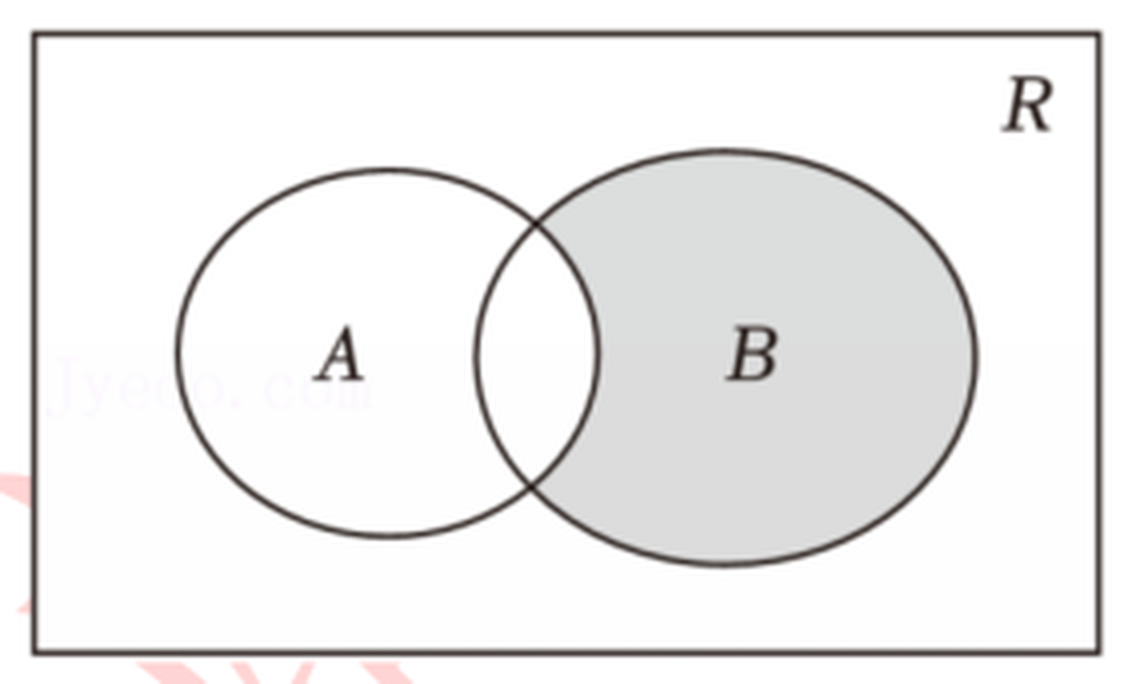
\includegraphics[width=0.30\textwidth]{figures/venn_Abar_cap_B.png}
\end{center}

\begin{enumerate}[label=(\arabic*)]
\item 若 $a=1$，求阴影部分表示的集合.
\item 若 $A\cap B=B$，求实数 $a$ 的取值范围.
\end{enumerate}

\ifanswer
\solbegin
\stepm{(1)}{因为 $\dfrac{2x-3}{x+5}\leqslant0$，
等价于 $\begin{cases}(2x-3)(x+5)\leqslant0\\ x+5\neq0\end{cases}$，}
\step{解得 $-5<x\leqslant\dfrac32$，即 $A=\left\{x\mid-5<x\leqslant\dfrac32\right\}$；}
\step{若 $a=1$，因为 $|x-1|<1$，等价于 $-1<x-1<1$，}
\step{解得 $0<x<2$，即 $B=\{x\mid0<x<2\}$.}
\step{由 Venn 图得阴影部分表示的集合为 $\overline{A}\cap B=\left(\dfrac32,2\right)$.}
\stepm{(2)}{由 (1) 得 $A=\left\{x\mid-5<x\leqslant\dfrac32\right\}$，}
\step{$B=\{x\mid|x-a|<1\}=\{x\mid-1+a<x<1+a\}\neq\varnothing$，}
\step{因为 $A\cap B=B$，所以 $B\sub A$，}
\step{所以 $\begin{cases}-5\leqslant-1+a\\ 1+a\leqslant\dfrac32\end{cases}$，
解得 $-4\leqslant a\leqslant\dfrac12$，}
\step{所以实数 $a$ 的取值范围为 $\left[-4,\dfrac12\right]$.}
\solend

\fi

\ansspace[6]

\item 设 $A=\{x\mid x^2-(m+3)x+2(m+1)=0,m\in\R\}$，
$B=\{x\mid 2x^2+(3n+1)x+2=0,n\in\R\}$.

\begin{enumerate}[label=(\arabic*)]
\item 是否存在 $m$、$n\in\R$，使得 $A=\{1,2\}$，$B=\varnothing$，说明理由；
\item 若 $A\cap B=A$，求 $m$、$n$ 的值.
\end{enumerate}

\ifanswer
\solbegin
\stepm{(1)}{由 $A=\{1,2\}$，得 $m=0$，}
\step{再由 $B=\varnothing$，得 $\Delta=(3n+1)^2-4\times2\times2=9n^2+6n-15<0$，}
\step{所以 $(3n+5)(n-1)<0$，解得 $-\dfrac53<n<1$，}
\step{故存在 $m=0$，$-\dfrac53<n<1$，使得 $A=\{1,2\}$，$B=\varnothing$.}
\stepm{(2)}{由 $x^2-(m+3)x+2(m+1)=0$，得 $x=2$ 或 $x=m+1$，}
\step{若 $A\cap B=A$，则 $A\sub B$，}
\step{将 $x=2$ 代入 $2x^2+(3n+1)x+2=0$，得 $n=-2$，}
\step{则 $B=\{x\mid 2x^2+(3n+1)x+2=0,n\in\R\}=\{x\mid 2x^2-5x+2=0\}
=\left\{2,\dfrac12\right\}$.}
\step{则 $m+1=\dfrac12$ 或 $m+1=2$，则 $m=-\dfrac12$ 或 $m=1$，
所以 $m=-\dfrac12$ 或 $m=1$，$n=-2$.}
\solend

\fi

\ansspace[6]

\item 已知陈述句 $\alpha$：关于 $x$ 的方程 $x^2-6x+m=0$ 有两个不同的正数根，陈述句
$\beta$：集合 $\{x\mid(m+1)x^2+4x+1=0,x\in\R\}$ 中至多有一个元素.

\begin{enumerate}[label=(\arabic*)]
\item 若 $\alpha$ 和 $\beta$ 都是真命题，求实数 $m$ 的取值范围；
\item 若 $\alpha$ 和 $\beta$ 至多有一个是假命题，求实数 $m$ 的取值范围.
\end{enumerate}

\ifanswer
\solbegin
\stepm{(1)}{因为关于 $x$ 的方程 $x^2-6x+m=0$ 有两个不同的正数根，}
\step{则 $\begin{cases}36-4m>0\\ m>0\end{cases}$，解得 $0<m<9$，}
\step{集合 $\{x\mid(m+1)x^2+4x+1=0,x\in\R\}$ 中至多有一个元素，}
\step{则 $m=-1$ 或 $\begin{cases}m+1\neq0\\ 16-4(m+1)\leqslant0\end{cases}$，
解得 $m\geqslant3$，}
\step{$\alpha$ 和 $\beta$ 都是真命题，所以实数 $m$ 的取值范围为 $\{m\mid3\leqslant m<9\}$}
\stepm{(2)}{由 (1) 得当 $\alpha$ 为假命题时，$m\leqslant0$ 或 $m\geqslant9$，}
\step{当 $\beta$ 为假命题时，$m<3$ 且 $m\neq-1$，}
\step{所以 $\alpha$ 和 $\beta$ 均为假命题时，$m$ 的范围是 $m\leqslant0$ 且 $m\neq-1$，}
\step{$\alpha$ 和 $\beta$ 至多有一个是假命题时，实数 $m$ 的取值范围为
$\{m\mid m>0$ 或 $m=-1\}$.}
\solend

\fi

\ansspace[6]

\item 已知符号 $[x]$ 表示不大于 $x$ 的最大整数 $(x\in\R)$，例如：$[1.3]=1$，
$[2]=2$，$[-1.2]=-2$.

\begin{enumerate}[label=(\arabic*)]
\item 已知方程 $[x]=3$，求该方程的解集；
\item 设方程 $\bigl[|x|+|x-1|\bigr]=3$ 的解集为 $A$，
集合 $B=\{x\mid 2x^2-11kx+15k^2\geqslant0\}$，若 $A\cup B=\R$，求实数 $k$ 的取值范围；
\item 在 (2) 的条件下，集合 $C=\{x\mid x^2-ax+1-2a\leqslant0,a\in\R\}$，是否存在实数
$a$，$A\cap C=A$，若存在，请求出实数 $a$ 的取值范围；若不存在，请说明理由.
\end{enumerate}

\ifanswer
\solbegin
\stepm{(1)}{方程 $[x]=3$，则 $x\in[3,4)$，所以该方程的解集为 $[3,4)$；}
\stepm{(2)}{因为 $\bigl[|x|+|x-1|\bigr]=3$，所以 $3\leqslant|x|+|x-1|<4$，}
\step{由绝对值不等式的几何意义得 $A=\left(-\dfrac32,-1\right]\cup\left[2,\dfrac52\right)$，}
\step{又 $B=\{x\mid 2x^2-11kx+15k^2\geqslant0\}=\{x\mid(2x-5k)(x-k)\geqslant0\}$，}
\step{当 $k=0$ 时，$B=\{x\mid 2x^2\geqslant0\}=\R$，则 $A\cup B=\R$，符合题意；}
\step{当 $k>0$ 时，$B=\left(-\infty,\dfrac{5k}{2}\right]\cup[3k,+\infty)$，
若 $A\cup B=\R$，}
\step{则 $\begin{cases}\dfrac{5k}{2}\geqslant2\\[2pt] 3k\leqslant\dfrac52\end{cases}$，
解得 $k\in\left[\dfrac45,\dfrac56\right]$；}
\step{当 $k<0$ 时，$B=(-\infty,3k]\cup\left[\dfrac{5k}{2},+\infty\right)$，
若 $A\cup B=\R$，}
\step{则 $\begin{cases}\dfrac{5k}{2}\leqslant-1\\[2pt] 3k\geqslant-\dfrac32\end{cases}$，
解得 $k\in\left[-\dfrac12,-\dfrac25\right]$.}
\step{综上所述，实数 $k$ 的取值范围为
$\left[-\dfrac12,-\dfrac25\right]\cup\{0\}\cup\left[\dfrac45,\dfrac56\right]$；}
\stepm{(3)}{因为 $A\cap C=A$，则 $A\sub C$ 且
$A=\left(-\dfrac32,-1\right]\cup\left[2,\dfrac52\right)$，}
\step{设集合 $C$ 的解集为 $(x_1,x_2)(x_1<x_2)$，}
\step{则 $\begin{cases}x_1\leqslant-\dfrac32\\[2pt] x_2\geqslant\dfrac52\end{cases}$，}
\step{所以
$\begin{cases}\Delta=a^2-4(1-2a)>0\\[2pt]
f\!\left(-\dfrac32\right)=\dfrac94+\dfrac32a+1-2a\leqslant0\\[4pt]
f\!\left(\dfrac52\right)=\dfrac{25}{4}-\dfrac52a+1-2a\leqslant0\end{cases}$，
解得 $a\geqslant\dfrac{13}{2}$，}
\step{故实数 $a$ 的取值范围为 $\left[\dfrac{13}{2},+\infty\right)$.}
\solend

\fi

\ansspace[6]

\item 非空有限集合 $S$ 是由若干个正实数组成，集合 $S$ 的元素个数不少于 $2$ 个. 对于任意
$a,b\in S,a\neq b$，若数 $a^b$ 或 $b^a$ 中至少有一个属于 $S$，则称集合 $S$ 是“好集”；
否则，称集合 $S$ 是“坏集”.

\begin{enumerate}[label=(\arabic*)]
\item 判断 $A=\{1,3,9\}$ 和 $B=\left\{1,\dfrac12,\dfrac14,\dfrac1{16}\right\}$ 是“好集”
还是“坏集”，并简单说明理由；
\item 题设的有限集 $S$ 中，既有大于 $1$ 的元素，又有小于 $1$ 的元素，证明：集合 $S$ 是
“坏集”；
\item 若题设中的 $a^b$ 或 $b^a$ 都属于 $S$，则称集合 $S$ 为“超级好集”，写出一个
“超级好集”（无须证明）.
\end{enumerate}

\ifanswer
\solbegin
\stepm{(1)}{$A=\{1,3,9\}$，$3^9\notin A$，$9^3\notin A$，所以 $A$ 是“坏集”，}
\step{从 $B$ 集合中任意取两个数字都满足需求，所以 $B$ 是“好集”.}
\stepm{(2)}{假设 $a$ 是 $S$ 中小于 $1$ 的元素中的最小元素，}
\step{$b$ 是 $S$ 中大于 $1$ 的元素中的最小元素，则 $a^b<a^1=a$，}
\step{所以 $a$ 就不是 $S$ 中小于 $1$ 的元素中的最小元素，即 $a^b\notin S$，}
\step{同理 $1=b^0<b^a<b^1=b$，所以 $b$ 就不是 $S$ 中大于 $1$ 的元素中的最小元素，}
\step{即 $b^a\notin S$，所以集合 $S$ 是“坏集”；}
\stepm{(3)}{首先 $S=\{1,a\}$（$a\neq1$ 且 $a>0$）是“超级好集”，}
\step{假设 $0<a<1$，由 (2) 得，$S$ 中不可能有大于 $1$ 的元素，}
\step{假设 $S$ 中有除 $a$ 之外的元素 $b\in S$（$a\neq b,b<1$），}
\step{假设 $a$ 是 $S$ 中小于 $1$ 的元素中的最大元素，$a^b>a^1=a$，}
\step{所以 $a$ 不是最大元素，所以 $a^b\notin S$，所以 $b\notin S$；}
\step{假设 $a>1$，由 (2) 得 $S$ 中不可能有小于 $1$ 的元素，}
\step{假设 $S$ 中有除 $a$ 之外的元素 $b$（$b>1$ 且 $b\neq a$），}
\step{假设 $a$ 是 $S$ 中大于 $1$ 的元素中的最小元素，则 $a^b>a^1=a$，}
\step{所以 $a$ 不是最小元素，即不存在 $b>1$，使得 $b\in S$，即 $b\notin S$，}
\step{综上，$S=\{1,a\}$（$a\neq1$ 且 $a>0$）.}
\solend

\fi

\ansspace*[10]

\end{enumerate}

\end{document}
"
% 紧凑版：xelatex "\def\iscompact{1}% 高一25_华师大二附中_周末作业3.tex
%   —— 高一上数学「2026-2027 年华师大二附中高一上周末作业 3」（试卷版/答案版）
% 试卷版：xelatex 高一25_华师大二附中_周末作业3.tex
% 答案版：xelatex "\def\isanswer{1}% 高一25_华师大二附中_周末作业3.tex
%   —— 高一上数学「2026-2027 年华师大二附中高一上周末作业 3」（试卷版/答案版）
% 试卷版：xelatex 高一25_华师大二附中_周末作业3.tex
% 答案版：xelatex "\def\isanswer{1}\input{高一25_华师大二附中_周末作业3.tex}"
% 紧凑版：xelatex "\def\iscompact{1}\input{高一25_华师大二附中_周末作业3.tex}"
%
% 原始材料是微信公众号图文（公众号「魔都数学加油站」连载「27学年高一 25」，2026-09-21 发布，
% 原文标题「27学年高一25——2026-2027年上海市华师大二附中高一上周末作业3」），
% 正文为 10 张 PNG 页（1080×1527，各页同尺寸）。原文本身就是一份**讲评版**——
% 题目下方直接印出【解析】（本卷无单独的【答案】行，填空题答案都写在解析里）。
% 试题文字与解析均照原卷录入，未改内容。卷面的粉色斜水印「魔都数学加油站」属水印，未录入。
%
% 卷首标题：原卷印作「2026-2027 年华师大二附中高一上周末作业 3」（公众号标题里的「上海市」
% 三字卷面标题行没有，本稿照卷面），年份区间按全稿惯例排 en dash，前缀照原卷保留「年」。
%
% 与原卷的排版差异（均已在 README「说明」中交代）：
%   ① 原文自**第 3 题**起（第 1、2 题未在该文中发布），故本稿题号亦自 3 起；
%   ② 原卷本就印有「一、填空题」「二、选择题」「三、解答题」三节标题，本稿照原卷分节，
%      只把标题改排成全稿统一的「大节标题」样式；
%   ③ 原卷第 13 题的答案「D」直接印在题干末尾的括号内，第 14—16 题的括号空着、答案写在
%      解析末句「故选 C／B」里；填空题的答案也都嵌在解析里，本稿统一改为试卷版隐去、
%      答案版以 \ans{} 给出（选择题另附【解析】），使两版彻底分离；
%   ④ 补集符号原卷一律作**上横线**（$\overline{A}$、$\overline{A\cup B}$），与同校的
%      高一14 同例，本稿照录（不改为 $\complement_U A$ 写法）；
%   ⑤ 原卷的实数集 R 斜体与粗体混用（第 17 题题干「全集为 R」作粗体，第 5、14 题与
%      第 16 题解析的 $R$ 为斜体），本稿按全稿惯例统一写作 $\R$；
%   ⑥ 原卷填空的横线约两个字宽，本稿按全稿惯例统一排 \blankline[4.4em]；
%   ⑦ 原卷未印副标题，本稿按全稿惯例补出副标题「集合与常用逻辑用语」；
%   ⑧ 第 17 题的 Venn 图原卷印在题干右侧（第 6 页），本稿移至题干之后；
%      图取原卷截图、4× LANCZOS 放大（figures/venn_Abar_cap_B.png，
%      阴影为 $B$ 中不含 $A\cap B$ 的部分，即 $\overline{A}\cap B$）。
%
% 原卷存疑两处（均照抄原卷、未改，见源码中该处上方注释）：
%   ① 第 8 题【解析】第二段「当 $\Delta=a^2-16>0$ 时，方程 $x^2+ax+4=0$ 有两个相同的根
%      $x_1$、$x_2$」——$\Delta>0$ 应为「两个**不**相同的根」（其自己的后文就把 $x_1$、$x_2$
%      当作可以不同的两个根在讨论），显系笔误；
%   ② 第 11 题【解析】先写「偶数必是 $2^{11}\cdot3^m\cdot337^n$，$m$、$n\in\N^*$」，
%      下一行又写「$0\leqslant m\leqslant10$，$0\leqslant n\leqslant10$，共有 121 种情况」
%      ——按 $\N^*$ 应从 1 起（至多 $10\times10=100$ 种），与 121（$=11\times11$，含 0）
%      对不上，两处至少有一处笔误。

\documentclass[a4paper,11pt]{article}
\usepackage{common}

\begin{document}

\examtitlest[3]{2026--2027 年华师大二附中高一上周末作业 3}{集合与常用逻辑用语}

\bigsec{一、填空题}

\begin{enumerate}
\setcounter{enumi}{2}

\item 设全集 $U=\{2,4,m^2+m-5\}$，集合 $A=\{2,1-m\}$，若 $\overline{A}=\{1\}$，则实数
$m=$ \blankline[4.4em].

\ifanswer
\solbegin
\step{因为 $\overline{A}=\{1\}$，所以 $1\in U$，$1\notin A$，}
\step{所以 $\begin{cases}m^2+m-5=1\\ 1-m\neq1\\ 1-m=4\end{cases}$，解得 $m=-3$.}
\solend

\fi

\item 已知条件 $\alpha$：$m<x\leqslant2m+5$，条件 $\beta$：$0\leqslant x\leqslant1$，
若 $\alpha$ 是 $\beta$ 的必要条件，则实数 $m$ 的取值范围为 \blankline[4.4em].

\ifanswer
\solbegin
\step{若 $\alpha$ 是 $\beta$ 的必要条件，则 $[0,1]\sub(m,2m+5]$，}
\step{所以 $\begin{cases}m<2m+5\\ m<0\\ 2m+5\geqslant1\end{cases}$，}
\step{解得 $-2\leqslant m<0$，故实数 $m$ 的取值范围为 $[-2,0)$.}
\solend

\fi

\item 已知 $\R$ 是全集，集合 $A=\{y\mid y=-x^2+1,x\in\R\}$，集合
$B=\{x\mid x=3+|a|,a\in\R\}$，则 $\overline{A\cup B}=$ \blankline[4.4em].

\ifanswer
\solbegin
\step{$A=\{y\mid y=-x^2+1,x\in\R\}=(-\infty,1]$，}
\step{$B=\{x\mid x=3+|a|,a\in\R\}=[3,+\infty)$，}
\step{所以 $\overline{A\cup B}=(1,3)$.}
\solend

\fi

\item 已知 $a$ 为常数，集合 $A=\{x\mid x^2+x-6=0\}$，集合 $B=\{x\mid ax-2=0\}$，且
$B\sub A$，则 $a$ 的所有取值构成的集合为 \blankline[4.4em].

\ifanswer
\solbegin
\step{集合 $A=\{-3,2\}$，因为 $B\sub A$，所以 $B=\varnothing$，$\{-3\}$，$\{2\}$，$\{-3,2\}$，}
\step{当 $B=\varnothing$ 时，$a=0$，当 $B=\{-3\}$ 时，$a=-\dfrac23$，当 $B=\{2\}$ 时，$a=1$，}
\step{当 $B=\{-3,2\}$ 时，不成立，故 $a$ 的取值集合为 $\left\{0,-\dfrac23,1\right\}$.}
\solend

\fi

\item 已知一元二次方程 $x^2+px+p=0$ 有两个不相等的实根分别为 $x_1$、$x_2$.
$A=x_1^2+x_2^2$，$B=x_1x_2(x_1+x_2)$，$A$ 与 $B$ 的大小为 \blankline[4.4em].

\ifanswer
\solbegin
\step{一元二次方程 $x^2+px+p=0$ 有两个不相等的实根分别为 $x_1$、$x_2$，}
\step{则 $\Delta=p^2-4p>0$，解得 $p<0$ 或 $p>4$，}
\step{由韦达定理得 $x_1+x_2=-p$，$x_1x_2=p$，}
\step{所以 $A=x_1^2+x_2^2=(x_1+x_2)^2-2x_1x_2=p^2-2p$，$B=x_1x_2(x_1+x_2)=-p^2$，}
\step{所以 $A-B=(p^2-2p)-(-p^2)=2p(p-1)$，}
\step{当 $p<0$ 时，则 $A-B>0$，故 $A>B$，}
\step{当 $p>4$ 时，则 $A-B>0$，故 $A>B$，}
\step{综上，$A=p^2-2p$，$B=-p^2$，且 $A>B$.}
\solend

\fi

\item 集合 $A=\{x\mid(x-1)(x^2+ax+4)=0,x\in\R\}$ 中所有元素之和为 $3$，则实数
$a=$ \blankline[4.4em].

\ifanswer
\solbegin
\step{当 $\Delta=a^2-16=0$ 时，方程 $x^2+ax+4=0$ 有两个相同的根 $-\dfrac a2$，}
\step{则 $A=\left\{1,-\dfrac a2\right\}$，故 $1-\dfrac a2=3$，解得 $a=-4$；}
% 注：下一行的「两个相同的根」系原卷笔误（△>0 应为「两个不相同的根」，其自己的后文
%     就把 x₁、x₂ 当作可以不同的两个根在讨论），照抄原卷、未改，见文件头「原卷存疑」①。
\step{当 $\Delta=a^2-16>0$ 时，方程 $x^2+ax+4=0$ 有两个相同的根 $x_1$、$x_2$，}
\step{若 $1$ 是方程 $x^2+ax+4=0$ 的根，则方程 $x^2+ax+4=0$ 的另一个根为 $4$，}
\step{则 $A=\{1,4\}$，不成立；}
\step{若 $1$ 不是方程 $x^2+ax+4=0$ 的根，则 $A=\{1,x_1,x_2\}$，则 $1+x_1+x_2=3$，}
\step{故 $x_1+x_2=2=-a$，故 $a=-2$（舍去）；}
\step{综上所述，$a=-4$.}
\solend

\fi

\item 已知集合 $A=\{x\mid x^2+2x-8\geqslant0\}$，$B=\{x\mid x^2-2ax+4\leqslant0\}$，
若 $a>0$，且 $A\cap B\cap\N$ 中恰有 $2$ 个元素，则 $a$ 的取值范围为 \blankline[4.4em].

\ifanswer
\solbegin
\step{由 $A$ 中不等式变形得 $(x-2)(x+4)\geqslant0$，解得 $x\leqslant-4$ 或 $x\geqslant2$，}
\step{即 $A=(-\infty,-4]\cup[2,+\infty)$，}
\step{设 $f(x)=x^2-2ax+4$，则 $f(x)$ 的轴对称 $x=a>0$，}
\step{且对应方程的根 $x_1$、$x_2$ 满足 $\begin{cases}x_1x_2=4\\ x_1+x_2>0\end{cases}$，}
\step{所以 $0<x_1\leqslant2\leqslant x_2$（取 $x_1\leqslant x_2$），}
\step{所以 $A\cap B\cap\N$ 中恰有的整数为 $2$，$3$，}
\step{所以 $\begin{cases}f(3)=9-6a+4\leqslant0\\ f(4)=16-8a+4>0\end{cases}$，}
\step{解得 $\dfrac{13}{6}\leqslant a<\dfrac52$，所以 $a$ 的取值范围为 $\left[\dfrac{13}{6},\dfrac52\right)$.}
\solend

\fi

\item 在三个关于 $x$ 的方程 $x^2-ax+4=0$，$x^2+(a-1)x+16=0$ 和
$x^2+2ax+3a+10=0$ 中至少有一个方程有实根，则实数 $a$ 的取值范围是 \blankline[4.4em].

\ifanswer
\solbegin
\step{当三个方程均无实根时，有}
\step{$\begin{cases}\Delta_1=a^2-16<0\\ \Delta_2=(a-1)^2-64<0\\ \Delta_3=4a^2-4(3a+10)<0\end{cases}$，}
\step{所以 $\begin{cases}-4<a<4\\ -7<a<9\\ -2<a<5\end{cases}$，}
\step{所以 $-2<a<4$，故三个方程均无实根时，$a$ 的取值范围为 $(-2,4)$，}
\step{所以三个方程中至少有一个方程有实根时，}
\step{实数 $a$ 的取值范围为 $(-\infty,-2]\cup[4,+\infty)$.}
\solend

\fi

% 注：下一行解析里的「m、n∈N*」与再下一行的「0≤m≤10，0≤n≤10，共有 121 种情况」
%     对不上（按 N* 应从 1 起，至多 10×10=100 种；121=11×11 含 0），系原卷自身矛盾，
%     照抄原卷、未改，见文件头「原卷存疑」②。
\item 若集合 $M=\{(x,y)\mid(x+1)+(x+2)+\cdots+(x+y)=2022^{10},x\in\Z,y\in\N^{*}\}$，
则集合 $M$ 中元素有 \blankline[4.4em] 个.

\ifanswer
\solbegin
\step{由题意得 $(x+1)+(x+2)+\cdots+(x+y)=\dfrac{y(2x+1+y)}{2}$，}
\step{所以 $y(2x+1+y)=2^{11}\cdot3^{10}\cdot337^{10}$，}
\step{因为 $y$ 与 $2x+1+y$ 必为一奇一偶，偶数必是 $2^{11}\cdot3^m\cdot337^n$，
$m$、$n\in\N^{*}$，}
\step{$0\leqslant m\leqslant10$，$0\leqslant n\leqslant10$，共有 $121$ 种情况，}
\step{因为 $y$ 与 $2x+1+y$ 奇偶未定，所以集合 $M$ 中元素只有 $242$ 个.}
\solend

\fi

\item 设集合 $M=\left\{x\mid m\leqslant x\leqslant m+\dfrac34\right\}$，
$N=\left\{x\mid n-\dfrac13\leqslant x\leqslant n\right\}$，且 $M$、$N$ 都是集合
$\{x\mid0\leqslant x\leqslant1\}$ 的子集，如果把 $b-a$ 叫做集合
$\{x\mid a\leqslant x\leqslant b\}$ 的长度，那么集合 $M\cap N$ 的长度的最小值是
\blankline[4.4em].

\ifanswer
\solbegin
\step{$M$ 的长度为 $\dfrac34$，$N$ 的长度为 $\dfrac13$，}
\step{当集合 $M\cap N$ 的长度的最小值时，$M$ 与 $N$ 应分别在区间 $[0,1]$ 的左右两端，}
\step{故 $M\cap N$ 的长度的最小值是 $\dfrac34+\dfrac13-1=\dfrac1{12}$.}
\solend

\fi

\end{enumerate}

\bigsec{二、选择题}

\begin{enumerate}
\setcounter{enumi}{12}

\item 直角坐标平面中除去两点 $A(1,1)$、$B(2,-2)$ 可用集合表示为\mbox{（\quad）}

\keepwithprev
A. $\{(x,y)\mid x\neq1,y\neq1,x\neq2,y\neq-2$\}\qquad
B. $\{(x,y)\mid\begin{cases}x\neq1\\ y\neq1\end{cases}$ 或 $\begin{cases}x\neq2\\ y\neq-2\end{cases}\}$

C. $\{(x,y)\mid[(x-1)^2+(y-1)^2][(x-2)^2+(y+2)^2]\neq0$\}

D. $\{(x,y)\mid[(x-1)^2+(y-1)^2]+[(x-2)^2+(y+2)^2]\neq0$\}

\ans{$D$}

\item 已知函数 $f(x)=x^2+nx$，记集合 $A=\{x\mid f(x)=0,x\in\R\}$，
$B=\{x\mid f(f(x))=0,x\in\R\}$，若 $A=B\neq\varnothing$，则 $n$ 的取值范围是\mbox{（\quad）}

\keepwithprev
A. $[0,4]$\qquad B. $(0,4)$\qquad C. $[0,4)$\qquad D. $(0,4]$

\ans{$C$}

\ifanswer
\solbegin
\step{$f(x)=x^2+nx$，$f[f(x)]=(x^2+nx)^2+n(x^2+nx)=(x^2+nx)(x^2+nx+n)$，}
\step{当 $n=0$ 时，$f(x)=x^2$，$f[f(x)]=x^4$，满足 $A=B$，此时 $n=0$；}
\step{当 $n\neq0$ 时，$0$、$-n$ 不是 $x^2+nx+n=0$ 的根，故 $\Delta=n^2-4n<0$，
解得 $0<n<4$，}
\step{综上所述，$n$ 的取值范围是 $[0,4)$. 故选 $C$.}
\solend

\fi

\item 设全集 $U=\{1,2,3,4,5,6,7,8,9,10\}$，给出条件：① $A\sub U$；②若 $x\in A$，
则 $2x\notin A$；③若 $x\in\overline{A}$，则 $2x\notin\overline{A}$.
那么同时满足三个条件的集合 $A$ 的个数为\mbox{（\quad）}

\keepwithprev
A. $0$ 个\qquad B. $16$ 个\qquad C. $32$ 个\qquad D. $64$ 个

\ans{$C$}

\ifanswer
\solbegin
\step{由① $A\sub U$；②若 $x\in A$，则 $2x\notin A$；③若 $x\in\overline{A}$，
则 $2x\notin\overline{A}$.}
\step{若 $1\in A$，则 $2\notin A$，即 $2\in\overline{A}$，则 $4\notin\overline{A}$，
即 $4\in A$，则 $8\notin A$，即 $8\in\overline{A}$；}
\step{若 $3\in A$，则 $6\notin A$，即 $6\in\overline{A}$；若 $5\in A$，则 $10\notin A$，
即 $10\in\overline{A}$，}
\step{故 $1$、$4$ 和 $2$、$8$ 分开，$3$ 和 $6$ 分开，$5$ 和 $10$ 分开，$7$ 和 $9$ 随意，}
\step{故同时满足三个条件的集合 $A$ 的个数为 $2\times2\times2\times2\times2=32$，
故选 $C$.}
\solend

\fi

\item 设集合 $P_1=\{x\mid x^2+ax+1>0\}$，$P_2=\{x\mid x^2+ax+2>0\}$，
$Q_1=\{x\mid x^2+x+b>0\}$，$Q_2=\{x\mid x^2+2x+b>0\}$，其中 $a$、$b\in\R$，
下列说法中正确的是\mbox{（\quad）}

\keepwithprev
A. 对任意 $a$，$P_1$ 是 $P_2$ 的子集，对任意的 $b$，$Q_1$ 不是 $Q_2$ 的子集

B. 对任意 $a$，$P_1$ 是 $P_2$ 的子集，存在 $b$，使得 $Q_1$ 是 $Q_2$ 的子集

C. 存在 $a$，使得 $P_1$ 不是 $P_2$ 的子集，对任意的 $b$，$Q_1$ 不是 $Q_2$ 的子集

D. 存在 $a$，使得 $P_1$ 不是 $P_2$ 的子集，存在 $b$，使得 $Q_1$ 是 $Q_2$ 的子集

\ans{$B$}

\ifanswer
\solbegin
\step{对于集合 $P_1=\{x\mid x^2+ax+1>0\}$，$P_2=\{x\mid x^2+ax+2>0\}$，}
\step{得当 $m\in P_1$ 时，即 $m^2+am+1>0$，得 $m^2+am+2>0$，}
\step{即有 $m\in P_2$，得对任意 $a$，$P_1$ 是 $P_2$ 的子集，}
\step{对于集合 $Q_1=\{x\mid x^2+x+b>0\}$，$Q_2=\{x\mid x^2+2x+b>0\}$，}
\step{当 $b=6$ 时，$Q_1=\{x\mid x^2+x+6>0\}=\R$，$Q_2=\{x\mid x^2+2x+6>0\}=\R$，}
\step{得 $Q_1$ 是 $Q_2$ 的子集，}
\step{当 $b=1$ 时，$Q_1=\{x\mid x^2+x+1>0\}=\R$，}
\step{$Q_2=\{x\mid x^2+2x+1>0\}=\{x\mid x\neq-1\}$，得 $Q_1$ 不是 $Q_2$ 的子集，}
\step{所以存在 $b$，使得 $Q_1$ 是 $Q_2$ 的子集，故选 $B$.}
\solend

\fi

\end{enumerate}

\bigsec{三、解答题}

\begin{enumerate}
\setcounter{enumi}{16}

\item 已知集合 $A=\left\{x\mid\dfrac{2x-3}{x+5}\leqslant0\right\}$，
$B=\{x\mid|x-a|<1\}$，全集为 $\R$.

\begin{center}
% 图取原卷截图、4× LANCZOS 放大（原卷把图印在题干右侧，本稿移至此处，见文件头⑧）。
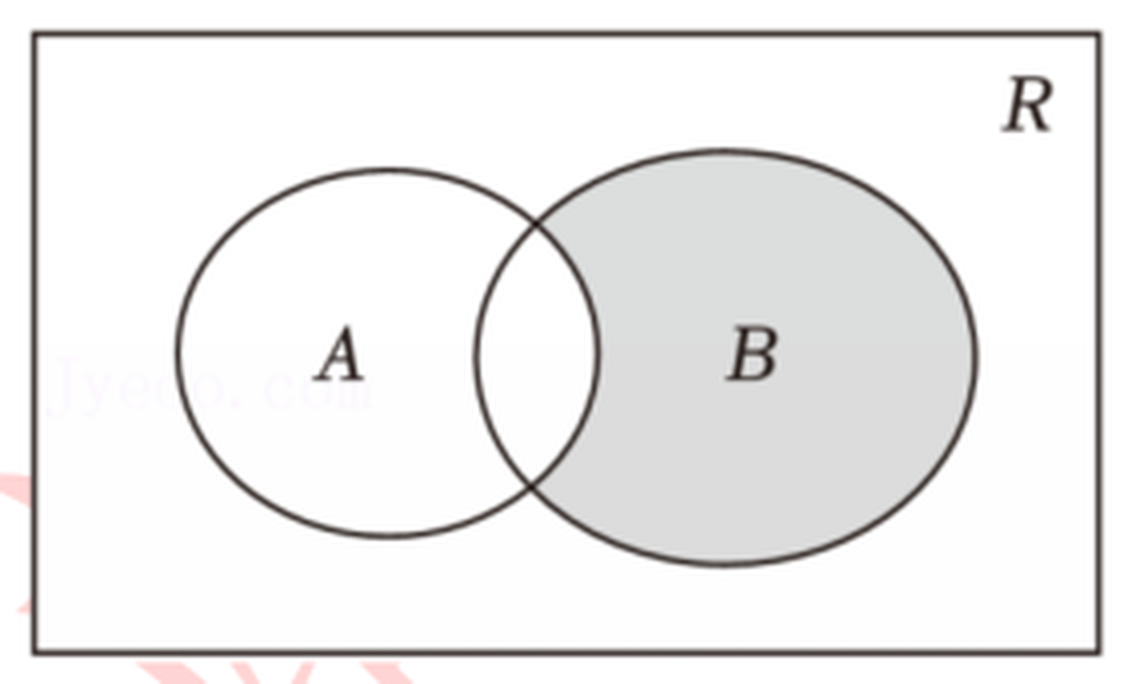
\includegraphics[width=0.30\textwidth]{figures/venn_Abar_cap_B.png}
\end{center}

\begin{enumerate}[label=(\arabic*)]
\item 若 $a=1$，求阴影部分表示的集合.
\item 若 $A\cap B=B$，求实数 $a$ 的取值范围.
\end{enumerate}

\ifanswer
\solbegin
\stepm{(1)}{因为 $\dfrac{2x-3}{x+5}\leqslant0$，
等价于 $\begin{cases}(2x-3)(x+5)\leqslant0\\ x+5\neq0\end{cases}$，}
\step{解得 $-5<x\leqslant\dfrac32$，即 $A=\left\{x\mid-5<x\leqslant\dfrac32\right\}$；}
\step{若 $a=1$，因为 $|x-1|<1$，等价于 $-1<x-1<1$，}
\step{解得 $0<x<2$，即 $B=\{x\mid0<x<2\}$.}
\step{由 Venn 图得阴影部分表示的集合为 $\overline{A}\cap B=\left(\dfrac32,2\right)$.}
\stepm{(2)}{由 (1) 得 $A=\left\{x\mid-5<x\leqslant\dfrac32\right\}$，}
\step{$B=\{x\mid|x-a|<1\}=\{x\mid-1+a<x<1+a\}\neq\varnothing$，}
\step{因为 $A\cap B=B$，所以 $B\sub A$，}
\step{所以 $\begin{cases}-5\leqslant-1+a\\ 1+a\leqslant\dfrac32\end{cases}$，
解得 $-4\leqslant a\leqslant\dfrac12$，}
\step{所以实数 $a$ 的取值范围为 $\left[-4,\dfrac12\right]$.}
\solend

\fi

\ansspace[6]

\item 设 $A=\{x\mid x^2-(m+3)x+2(m+1)=0,m\in\R\}$，
$B=\{x\mid 2x^2+(3n+1)x+2=0,n\in\R\}$.

\begin{enumerate}[label=(\arabic*)]
\item 是否存在 $m$、$n\in\R$，使得 $A=\{1,2\}$，$B=\varnothing$，说明理由；
\item 若 $A\cap B=A$，求 $m$、$n$ 的值.
\end{enumerate}

\ifanswer
\solbegin
\stepm{(1)}{由 $A=\{1,2\}$，得 $m=0$，}
\step{再由 $B=\varnothing$，得 $\Delta=(3n+1)^2-4\times2\times2=9n^2+6n-15<0$，}
\step{所以 $(3n+5)(n-1)<0$，解得 $-\dfrac53<n<1$，}
\step{故存在 $m=0$，$-\dfrac53<n<1$，使得 $A=\{1,2\}$，$B=\varnothing$.}
\stepm{(2)}{由 $x^2-(m+3)x+2(m+1)=0$，得 $x=2$ 或 $x=m+1$，}
\step{若 $A\cap B=A$，则 $A\sub B$，}
\step{将 $x=2$ 代入 $2x^2+(3n+1)x+2=0$，得 $n=-2$，}
\step{则 $B=\{x\mid 2x^2+(3n+1)x+2=0,n\in\R\}=\{x\mid 2x^2-5x+2=0\}
=\left\{2,\dfrac12\right\}$.}
\step{则 $m+1=\dfrac12$ 或 $m+1=2$，则 $m=-\dfrac12$ 或 $m=1$，
所以 $m=-\dfrac12$ 或 $m=1$，$n=-2$.}
\solend

\fi

\ansspace[6]

\item 已知陈述句 $\alpha$：关于 $x$ 的方程 $x^2-6x+m=0$ 有两个不同的正数根，陈述句
$\beta$：集合 $\{x\mid(m+1)x^2+4x+1=0,x\in\R\}$ 中至多有一个元素.

\begin{enumerate}[label=(\arabic*)]
\item 若 $\alpha$ 和 $\beta$ 都是真命题，求实数 $m$ 的取值范围；
\item 若 $\alpha$ 和 $\beta$ 至多有一个是假命题，求实数 $m$ 的取值范围.
\end{enumerate}

\ifanswer
\solbegin
\stepm{(1)}{因为关于 $x$ 的方程 $x^2-6x+m=0$ 有两个不同的正数根，}
\step{则 $\begin{cases}36-4m>0\\ m>0\end{cases}$，解得 $0<m<9$，}
\step{集合 $\{x\mid(m+1)x^2+4x+1=0,x\in\R\}$ 中至多有一个元素，}
\step{则 $m=-1$ 或 $\begin{cases}m+1\neq0\\ 16-4(m+1)\leqslant0\end{cases}$，
解得 $m\geqslant3$，}
\step{$\alpha$ 和 $\beta$ 都是真命题，所以实数 $m$ 的取值范围为 $\{m\mid3\leqslant m<9\}$}
\stepm{(2)}{由 (1) 得当 $\alpha$ 为假命题时，$m\leqslant0$ 或 $m\geqslant9$，}
\step{当 $\beta$ 为假命题时，$m<3$ 且 $m\neq-1$，}
\step{所以 $\alpha$ 和 $\beta$ 均为假命题时，$m$ 的范围是 $m\leqslant0$ 且 $m\neq-1$，}
\step{$\alpha$ 和 $\beta$ 至多有一个是假命题时，实数 $m$ 的取值范围为
$\{m\mid m>0$ 或 $m=-1\}$.}
\solend

\fi

\ansspace[6]

\item 已知符号 $[x]$ 表示不大于 $x$ 的最大整数 $(x\in\R)$，例如：$[1.3]=1$，
$[2]=2$，$[-1.2]=-2$.

\begin{enumerate}[label=(\arabic*)]
\item 已知方程 $[x]=3$，求该方程的解集；
\item 设方程 $\bigl[|x|+|x-1|\bigr]=3$ 的解集为 $A$，
集合 $B=\{x\mid 2x^2-11kx+15k^2\geqslant0\}$，若 $A\cup B=\R$，求实数 $k$ 的取值范围；
\item 在 (2) 的条件下，集合 $C=\{x\mid x^2-ax+1-2a\leqslant0,a\in\R\}$，是否存在实数
$a$，$A\cap C=A$，若存在，请求出实数 $a$ 的取值范围；若不存在，请说明理由.
\end{enumerate}

\ifanswer
\solbegin
\stepm{(1)}{方程 $[x]=3$，则 $x\in[3,4)$，所以该方程的解集为 $[3,4)$；}
\stepm{(2)}{因为 $\bigl[|x|+|x-1|\bigr]=3$，所以 $3\leqslant|x|+|x-1|<4$，}
\step{由绝对值不等式的几何意义得 $A=\left(-\dfrac32,-1\right]\cup\left[2,\dfrac52\right)$，}
\step{又 $B=\{x\mid 2x^2-11kx+15k^2\geqslant0\}=\{x\mid(2x-5k)(x-k)\geqslant0\}$，}
\step{当 $k=0$ 时，$B=\{x\mid 2x^2\geqslant0\}=\R$，则 $A\cup B=\R$，符合题意；}
\step{当 $k>0$ 时，$B=\left(-\infty,\dfrac{5k}{2}\right]\cup[3k,+\infty)$，
若 $A\cup B=\R$，}
\step{则 $\begin{cases}\dfrac{5k}{2}\geqslant2\\[2pt] 3k\leqslant\dfrac52\end{cases}$，
解得 $k\in\left[\dfrac45,\dfrac56\right]$；}
\step{当 $k<0$ 时，$B=(-\infty,3k]\cup\left[\dfrac{5k}{2},+\infty\right)$，
若 $A\cup B=\R$，}
\step{则 $\begin{cases}\dfrac{5k}{2}\leqslant-1\\[2pt] 3k\geqslant-\dfrac32\end{cases}$，
解得 $k\in\left[-\dfrac12,-\dfrac25\right]$.}
\step{综上所述，实数 $k$ 的取值范围为
$\left[-\dfrac12,-\dfrac25\right]\cup\{0\}\cup\left[\dfrac45,\dfrac56\right]$；}
\stepm{(3)}{因为 $A\cap C=A$，则 $A\sub C$ 且
$A=\left(-\dfrac32,-1\right]\cup\left[2,\dfrac52\right)$，}
\step{设集合 $C$ 的解集为 $(x_1,x_2)(x_1<x_2)$，}
\step{则 $\begin{cases}x_1\leqslant-\dfrac32\\[2pt] x_2\geqslant\dfrac52\end{cases}$，}
\step{所以
$\begin{cases}\Delta=a^2-4(1-2a)>0\\[2pt]
f\!\left(-\dfrac32\right)=\dfrac94+\dfrac32a+1-2a\leqslant0\\[4pt]
f\!\left(\dfrac52\right)=\dfrac{25}{4}-\dfrac52a+1-2a\leqslant0\end{cases}$，
解得 $a\geqslant\dfrac{13}{2}$，}
\step{故实数 $a$ 的取值范围为 $\left[\dfrac{13}{2},+\infty\right)$.}
\solend

\fi

\ansspace[6]

\item 非空有限集合 $S$ 是由若干个正实数组成，集合 $S$ 的元素个数不少于 $2$ 个. 对于任意
$a,b\in S,a\neq b$，若数 $a^b$ 或 $b^a$ 中至少有一个属于 $S$，则称集合 $S$ 是“好集”；
否则，称集合 $S$ 是“坏集”.

\begin{enumerate}[label=(\arabic*)]
\item 判断 $A=\{1,3,9\}$ 和 $B=\left\{1,\dfrac12,\dfrac14,\dfrac1{16}\right\}$ 是“好集”
还是“坏集”，并简单说明理由；
\item 题设的有限集 $S$ 中，既有大于 $1$ 的元素，又有小于 $1$ 的元素，证明：集合 $S$ 是
“坏集”；
\item 若题设中的 $a^b$ 或 $b^a$ 都属于 $S$，则称集合 $S$ 为“超级好集”，写出一个
“超级好集”（无须证明）.
\end{enumerate}

\ifanswer
\solbegin
\stepm{(1)}{$A=\{1,3,9\}$，$3^9\notin A$，$9^3\notin A$，所以 $A$ 是“坏集”，}
\step{从 $B$ 集合中任意取两个数字都满足需求，所以 $B$ 是“好集”.}
\stepm{(2)}{假设 $a$ 是 $S$ 中小于 $1$ 的元素中的最小元素，}
\step{$b$ 是 $S$ 中大于 $1$ 的元素中的最小元素，则 $a^b<a^1=a$，}
\step{所以 $a$ 就不是 $S$ 中小于 $1$ 的元素中的最小元素，即 $a^b\notin S$，}
\step{同理 $1=b^0<b^a<b^1=b$，所以 $b$ 就不是 $S$ 中大于 $1$ 的元素中的最小元素，}
\step{即 $b^a\notin S$，所以集合 $S$ 是“坏集”；}
\stepm{(3)}{首先 $S=\{1,a\}$（$a\neq1$ 且 $a>0$）是“超级好集”，}
\step{假设 $0<a<1$，由 (2) 得，$S$ 中不可能有大于 $1$ 的元素，}
\step{假设 $S$ 中有除 $a$ 之外的元素 $b\in S$（$a\neq b,b<1$），}
\step{假设 $a$ 是 $S$ 中小于 $1$ 的元素中的最大元素，$a^b>a^1=a$，}
\step{所以 $a$ 不是最大元素，所以 $a^b\notin S$，所以 $b\notin S$；}
\step{假设 $a>1$，由 (2) 得 $S$ 中不可能有小于 $1$ 的元素，}
\step{假设 $S$ 中有除 $a$ 之外的元素 $b$（$b>1$ 且 $b\neq a$），}
\step{假设 $a$ 是 $S$ 中大于 $1$ 的元素中的最小元素，则 $a^b>a^1=a$，}
\step{所以 $a$ 不是最小元素，即不存在 $b>1$，使得 $b\in S$，即 $b\notin S$，}
\step{综上，$S=\{1,a\}$（$a\neq1$ 且 $a>0$）.}
\solend

\fi

\ansspace*[10]

\end{enumerate}

\end{document}
"
% 紧凑版：xelatex "\def\iscompact{1}% 高一25_华师大二附中_周末作业3.tex
%   —— 高一上数学「2026-2027 年华师大二附中高一上周末作业 3」（试卷版/答案版）
% 试卷版：xelatex 高一25_华师大二附中_周末作业3.tex
% 答案版：xelatex "\def\isanswer{1}\input{高一25_华师大二附中_周末作业3.tex}"
% 紧凑版：xelatex "\def\iscompact{1}\input{高一25_华师大二附中_周末作业3.tex}"
%
% 原始材料是微信公众号图文（公众号「魔都数学加油站」连载「27学年高一 25」，2026-09-21 发布，
% 原文标题「27学年高一25——2026-2027年上海市华师大二附中高一上周末作业3」），
% 正文为 10 张 PNG 页（1080×1527，各页同尺寸）。原文本身就是一份**讲评版**——
% 题目下方直接印出【解析】（本卷无单独的【答案】行，填空题答案都写在解析里）。
% 试题文字与解析均照原卷录入，未改内容。卷面的粉色斜水印「魔都数学加油站」属水印，未录入。
%
% 卷首标题：原卷印作「2026-2027 年华师大二附中高一上周末作业 3」（公众号标题里的「上海市」
% 三字卷面标题行没有，本稿照卷面），年份区间按全稿惯例排 en dash，前缀照原卷保留「年」。
%
% 与原卷的排版差异（均已在 README「说明」中交代）：
%   ① 原文自**第 3 题**起（第 1、2 题未在该文中发布），故本稿题号亦自 3 起；
%   ② 原卷本就印有「一、填空题」「二、选择题」「三、解答题」三节标题，本稿照原卷分节，
%      只把标题改排成全稿统一的「大节标题」样式；
%   ③ 原卷第 13 题的答案「D」直接印在题干末尾的括号内，第 14—16 题的括号空着、答案写在
%      解析末句「故选 C／B」里；填空题的答案也都嵌在解析里，本稿统一改为试卷版隐去、
%      答案版以 \ans{} 给出（选择题另附【解析】），使两版彻底分离；
%   ④ 补集符号原卷一律作**上横线**（$\overline{A}$、$\overline{A\cup B}$），与同校的
%      高一14 同例，本稿照录（不改为 $\complement_U A$ 写法）；
%   ⑤ 原卷的实数集 R 斜体与粗体混用（第 17 题题干「全集为 R」作粗体，第 5、14 题与
%      第 16 题解析的 $R$ 为斜体），本稿按全稿惯例统一写作 $\R$；
%   ⑥ 原卷填空的横线约两个字宽，本稿按全稿惯例统一排 \blankline[4.4em]；
%   ⑦ 原卷未印副标题，本稿按全稿惯例补出副标题「集合与常用逻辑用语」；
%   ⑧ 第 17 题的 Venn 图原卷印在题干右侧（第 6 页），本稿移至题干之后；
%      图取原卷截图、4× LANCZOS 放大（figures/venn_Abar_cap_B.png，
%      阴影为 $B$ 中不含 $A\cap B$ 的部分，即 $\overline{A}\cap B$）。
%
% 原卷存疑两处（均照抄原卷、未改，见源码中该处上方注释）：
%   ① 第 8 题【解析】第二段「当 $\Delta=a^2-16>0$ 时，方程 $x^2+ax+4=0$ 有两个相同的根
%      $x_1$、$x_2$」——$\Delta>0$ 应为「两个**不**相同的根」（其自己的后文就把 $x_1$、$x_2$
%      当作可以不同的两个根在讨论），显系笔误；
%   ② 第 11 题【解析】先写「偶数必是 $2^{11}\cdot3^m\cdot337^n$，$m$、$n\in\N^*$」，
%      下一行又写「$0\leqslant m\leqslant10$，$0\leqslant n\leqslant10$，共有 121 种情况」
%      ——按 $\N^*$ 应从 1 起（至多 $10\times10=100$ 种），与 121（$=11\times11$，含 0）
%      对不上，两处至少有一处笔误。

\documentclass[a4paper,11pt]{article}
\usepackage{common}

\begin{document}

\examtitlest[3]{2026--2027 年华师大二附中高一上周末作业 3}{集合与常用逻辑用语}

\bigsec{一、填空题}

\begin{enumerate}
\setcounter{enumi}{2}

\item 设全集 $U=\{2,4,m^2+m-5\}$，集合 $A=\{2,1-m\}$，若 $\overline{A}=\{1\}$，则实数
$m=$ \blankline[4.4em].

\ifanswer
\solbegin
\step{因为 $\overline{A}=\{1\}$，所以 $1\in U$，$1\notin A$，}
\step{所以 $\begin{cases}m^2+m-5=1\\ 1-m\neq1\\ 1-m=4\end{cases}$，解得 $m=-3$.}
\solend

\fi

\item 已知条件 $\alpha$：$m<x\leqslant2m+5$，条件 $\beta$：$0\leqslant x\leqslant1$，
若 $\alpha$ 是 $\beta$ 的必要条件，则实数 $m$ 的取值范围为 \blankline[4.4em].

\ifanswer
\solbegin
\step{若 $\alpha$ 是 $\beta$ 的必要条件，则 $[0,1]\sub(m,2m+5]$，}
\step{所以 $\begin{cases}m<2m+5\\ m<0\\ 2m+5\geqslant1\end{cases}$，}
\step{解得 $-2\leqslant m<0$，故实数 $m$ 的取值范围为 $[-2,0)$.}
\solend

\fi

\item 已知 $\R$ 是全集，集合 $A=\{y\mid y=-x^2+1,x\in\R\}$，集合
$B=\{x\mid x=3+|a|,a\in\R\}$，则 $\overline{A\cup B}=$ \blankline[4.4em].

\ifanswer
\solbegin
\step{$A=\{y\mid y=-x^2+1,x\in\R\}=(-\infty,1]$，}
\step{$B=\{x\mid x=3+|a|,a\in\R\}=[3,+\infty)$，}
\step{所以 $\overline{A\cup B}=(1,3)$.}
\solend

\fi

\item 已知 $a$ 为常数，集合 $A=\{x\mid x^2+x-6=0\}$，集合 $B=\{x\mid ax-2=0\}$，且
$B\sub A$，则 $a$ 的所有取值构成的集合为 \blankline[4.4em].

\ifanswer
\solbegin
\step{集合 $A=\{-3,2\}$，因为 $B\sub A$，所以 $B=\varnothing$，$\{-3\}$，$\{2\}$，$\{-3,2\}$，}
\step{当 $B=\varnothing$ 时，$a=0$，当 $B=\{-3\}$ 时，$a=-\dfrac23$，当 $B=\{2\}$ 时，$a=1$，}
\step{当 $B=\{-3,2\}$ 时，不成立，故 $a$ 的取值集合为 $\left\{0,-\dfrac23,1\right\}$.}
\solend

\fi

\item 已知一元二次方程 $x^2+px+p=0$ 有两个不相等的实根分别为 $x_1$、$x_2$.
$A=x_1^2+x_2^2$，$B=x_1x_2(x_1+x_2)$，$A$ 与 $B$ 的大小为 \blankline[4.4em].

\ifanswer
\solbegin
\step{一元二次方程 $x^2+px+p=0$ 有两个不相等的实根分别为 $x_1$、$x_2$，}
\step{则 $\Delta=p^2-4p>0$，解得 $p<0$ 或 $p>4$，}
\step{由韦达定理得 $x_1+x_2=-p$，$x_1x_2=p$，}
\step{所以 $A=x_1^2+x_2^2=(x_1+x_2)^2-2x_1x_2=p^2-2p$，$B=x_1x_2(x_1+x_2)=-p^2$，}
\step{所以 $A-B=(p^2-2p)-(-p^2)=2p(p-1)$，}
\step{当 $p<0$ 时，则 $A-B>0$，故 $A>B$，}
\step{当 $p>4$ 时，则 $A-B>0$，故 $A>B$，}
\step{综上，$A=p^2-2p$，$B=-p^2$，且 $A>B$.}
\solend

\fi

\item 集合 $A=\{x\mid(x-1)(x^2+ax+4)=0,x\in\R\}$ 中所有元素之和为 $3$，则实数
$a=$ \blankline[4.4em].

\ifanswer
\solbegin
\step{当 $\Delta=a^2-16=0$ 时，方程 $x^2+ax+4=0$ 有两个相同的根 $-\dfrac a2$，}
\step{则 $A=\left\{1,-\dfrac a2\right\}$，故 $1-\dfrac a2=3$，解得 $a=-4$；}
% 注：下一行的「两个相同的根」系原卷笔误（△>0 应为「两个不相同的根」，其自己的后文
%     就把 x₁、x₂ 当作可以不同的两个根在讨论），照抄原卷、未改，见文件头「原卷存疑」①。
\step{当 $\Delta=a^2-16>0$ 时，方程 $x^2+ax+4=0$ 有两个相同的根 $x_1$、$x_2$，}
\step{若 $1$ 是方程 $x^2+ax+4=0$ 的根，则方程 $x^2+ax+4=0$ 的另一个根为 $4$，}
\step{则 $A=\{1,4\}$，不成立；}
\step{若 $1$ 不是方程 $x^2+ax+4=0$ 的根，则 $A=\{1,x_1,x_2\}$，则 $1+x_1+x_2=3$，}
\step{故 $x_1+x_2=2=-a$，故 $a=-2$（舍去）；}
\step{综上所述，$a=-4$.}
\solend

\fi

\item 已知集合 $A=\{x\mid x^2+2x-8\geqslant0\}$，$B=\{x\mid x^2-2ax+4\leqslant0\}$，
若 $a>0$，且 $A\cap B\cap\N$ 中恰有 $2$ 个元素，则 $a$ 的取值范围为 \blankline[4.4em].

\ifanswer
\solbegin
\step{由 $A$ 中不等式变形得 $(x-2)(x+4)\geqslant0$，解得 $x\leqslant-4$ 或 $x\geqslant2$，}
\step{即 $A=(-\infty,-4]\cup[2,+\infty)$，}
\step{设 $f(x)=x^2-2ax+4$，则 $f(x)$ 的轴对称 $x=a>0$，}
\step{且对应方程的根 $x_1$、$x_2$ 满足 $\begin{cases}x_1x_2=4\\ x_1+x_2>0\end{cases}$，}
\step{所以 $0<x_1\leqslant2\leqslant x_2$（取 $x_1\leqslant x_2$），}
\step{所以 $A\cap B\cap\N$ 中恰有的整数为 $2$，$3$，}
\step{所以 $\begin{cases}f(3)=9-6a+4\leqslant0\\ f(4)=16-8a+4>0\end{cases}$，}
\step{解得 $\dfrac{13}{6}\leqslant a<\dfrac52$，所以 $a$ 的取值范围为 $\left[\dfrac{13}{6},\dfrac52\right)$.}
\solend

\fi

\item 在三个关于 $x$ 的方程 $x^2-ax+4=0$，$x^2+(a-1)x+16=0$ 和
$x^2+2ax+3a+10=0$ 中至少有一个方程有实根，则实数 $a$ 的取值范围是 \blankline[4.4em].

\ifanswer
\solbegin
\step{当三个方程均无实根时，有}
\step{$\begin{cases}\Delta_1=a^2-16<0\\ \Delta_2=(a-1)^2-64<0\\ \Delta_3=4a^2-4(3a+10)<0\end{cases}$，}
\step{所以 $\begin{cases}-4<a<4\\ -7<a<9\\ -2<a<5\end{cases}$，}
\step{所以 $-2<a<4$，故三个方程均无实根时，$a$ 的取值范围为 $(-2,4)$，}
\step{所以三个方程中至少有一个方程有实根时，}
\step{实数 $a$ 的取值范围为 $(-\infty,-2]\cup[4,+\infty)$.}
\solend

\fi

% 注：下一行解析里的「m、n∈N*」与再下一行的「0≤m≤10，0≤n≤10，共有 121 种情况」
%     对不上（按 N* 应从 1 起，至多 10×10=100 种；121=11×11 含 0），系原卷自身矛盾，
%     照抄原卷、未改，见文件头「原卷存疑」②。
\item 若集合 $M=\{(x,y)\mid(x+1)+(x+2)+\cdots+(x+y)=2022^{10},x\in\Z,y\in\N^{*}\}$，
则集合 $M$ 中元素有 \blankline[4.4em] 个.

\ifanswer
\solbegin
\step{由题意得 $(x+1)+(x+2)+\cdots+(x+y)=\dfrac{y(2x+1+y)}{2}$，}
\step{所以 $y(2x+1+y)=2^{11}\cdot3^{10}\cdot337^{10}$，}
\step{因为 $y$ 与 $2x+1+y$ 必为一奇一偶，偶数必是 $2^{11}\cdot3^m\cdot337^n$，
$m$、$n\in\N^{*}$，}
\step{$0\leqslant m\leqslant10$，$0\leqslant n\leqslant10$，共有 $121$ 种情况，}
\step{因为 $y$ 与 $2x+1+y$ 奇偶未定，所以集合 $M$ 中元素只有 $242$ 个.}
\solend

\fi

\item 设集合 $M=\left\{x\mid m\leqslant x\leqslant m+\dfrac34\right\}$，
$N=\left\{x\mid n-\dfrac13\leqslant x\leqslant n\right\}$，且 $M$、$N$ 都是集合
$\{x\mid0\leqslant x\leqslant1\}$ 的子集，如果把 $b-a$ 叫做集合
$\{x\mid a\leqslant x\leqslant b\}$ 的长度，那么集合 $M\cap N$ 的长度的最小值是
\blankline[4.4em].

\ifanswer
\solbegin
\step{$M$ 的长度为 $\dfrac34$，$N$ 的长度为 $\dfrac13$，}
\step{当集合 $M\cap N$ 的长度的最小值时，$M$ 与 $N$ 应分别在区间 $[0,1]$ 的左右两端，}
\step{故 $M\cap N$ 的长度的最小值是 $\dfrac34+\dfrac13-1=\dfrac1{12}$.}
\solend

\fi

\end{enumerate}

\bigsec{二、选择题}

\begin{enumerate}
\setcounter{enumi}{12}

\item 直角坐标平面中除去两点 $A(1,1)$、$B(2,-2)$ 可用集合表示为\mbox{（\quad）}

\keepwithprev
A. $\{(x,y)\mid x\neq1,y\neq1,x\neq2,y\neq-2$\}\qquad
B. $\{(x,y)\mid\begin{cases}x\neq1\\ y\neq1\end{cases}$ 或 $\begin{cases}x\neq2\\ y\neq-2\end{cases}\}$

C. $\{(x,y)\mid[(x-1)^2+(y-1)^2][(x-2)^2+(y+2)^2]\neq0$\}

D. $\{(x,y)\mid[(x-1)^2+(y-1)^2]+[(x-2)^2+(y+2)^2]\neq0$\}

\ans{$D$}

\item 已知函数 $f(x)=x^2+nx$，记集合 $A=\{x\mid f(x)=0,x\in\R\}$，
$B=\{x\mid f(f(x))=0,x\in\R\}$，若 $A=B\neq\varnothing$，则 $n$ 的取值范围是\mbox{（\quad）}

\keepwithprev
A. $[0,4]$\qquad B. $(0,4)$\qquad C. $[0,4)$\qquad D. $(0,4]$

\ans{$C$}

\ifanswer
\solbegin
\step{$f(x)=x^2+nx$，$f[f(x)]=(x^2+nx)^2+n(x^2+nx)=(x^2+nx)(x^2+nx+n)$，}
\step{当 $n=0$ 时，$f(x)=x^2$，$f[f(x)]=x^4$，满足 $A=B$，此时 $n=0$；}
\step{当 $n\neq0$ 时，$0$、$-n$ 不是 $x^2+nx+n=0$ 的根，故 $\Delta=n^2-4n<0$，
解得 $0<n<4$，}
\step{综上所述，$n$ 的取值范围是 $[0,4)$. 故选 $C$.}
\solend

\fi

\item 设全集 $U=\{1,2,3,4,5,6,7,8,9,10\}$，给出条件：① $A\sub U$；②若 $x\in A$，
则 $2x\notin A$；③若 $x\in\overline{A}$，则 $2x\notin\overline{A}$.
那么同时满足三个条件的集合 $A$ 的个数为\mbox{（\quad）}

\keepwithprev
A. $0$ 个\qquad B. $16$ 个\qquad C. $32$ 个\qquad D. $64$ 个

\ans{$C$}

\ifanswer
\solbegin
\step{由① $A\sub U$；②若 $x\in A$，则 $2x\notin A$；③若 $x\in\overline{A}$，
则 $2x\notin\overline{A}$.}
\step{若 $1\in A$，则 $2\notin A$，即 $2\in\overline{A}$，则 $4\notin\overline{A}$，
即 $4\in A$，则 $8\notin A$，即 $8\in\overline{A}$；}
\step{若 $3\in A$，则 $6\notin A$，即 $6\in\overline{A}$；若 $5\in A$，则 $10\notin A$，
即 $10\in\overline{A}$，}
\step{故 $1$、$4$ 和 $2$、$8$ 分开，$3$ 和 $6$ 分开，$5$ 和 $10$ 分开，$7$ 和 $9$ 随意，}
\step{故同时满足三个条件的集合 $A$ 的个数为 $2\times2\times2\times2\times2=32$，
故选 $C$.}
\solend

\fi

\item 设集合 $P_1=\{x\mid x^2+ax+1>0\}$，$P_2=\{x\mid x^2+ax+2>0\}$，
$Q_1=\{x\mid x^2+x+b>0\}$，$Q_2=\{x\mid x^2+2x+b>0\}$，其中 $a$、$b\in\R$，
下列说法中正确的是\mbox{（\quad）}

\keepwithprev
A. 对任意 $a$，$P_1$ 是 $P_2$ 的子集，对任意的 $b$，$Q_1$ 不是 $Q_2$ 的子集

B. 对任意 $a$，$P_1$ 是 $P_2$ 的子集，存在 $b$，使得 $Q_1$ 是 $Q_2$ 的子集

C. 存在 $a$，使得 $P_1$ 不是 $P_2$ 的子集，对任意的 $b$，$Q_1$ 不是 $Q_2$ 的子集

D. 存在 $a$，使得 $P_1$ 不是 $P_2$ 的子集，存在 $b$，使得 $Q_1$ 是 $Q_2$ 的子集

\ans{$B$}

\ifanswer
\solbegin
\step{对于集合 $P_1=\{x\mid x^2+ax+1>0\}$，$P_2=\{x\mid x^2+ax+2>0\}$，}
\step{得当 $m\in P_1$ 时，即 $m^2+am+1>0$，得 $m^2+am+2>0$，}
\step{即有 $m\in P_2$，得对任意 $a$，$P_1$ 是 $P_2$ 的子集，}
\step{对于集合 $Q_1=\{x\mid x^2+x+b>0\}$，$Q_2=\{x\mid x^2+2x+b>0\}$，}
\step{当 $b=6$ 时，$Q_1=\{x\mid x^2+x+6>0\}=\R$，$Q_2=\{x\mid x^2+2x+6>0\}=\R$，}
\step{得 $Q_1$ 是 $Q_2$ 的子集，}
\step{当 $b=1$ 时，$Q_1=\{x\mid x^2+x+1>0\}=\R$，}
\step{$Q_2=\{x\mid x^2+2x+1>0\}=\{x\mid x\neq-1\}$，得 $Q_1$ 不是 $Q_2$ 的子集，}
\step{所以存在 $b$，使得 $Q_1$ 是 $Q_2$ 的子集，故选 $B$.}
\solend

\fi

\end{enumerate}

\bigsec{三、解答题}

\begin{enumerate}
\setcounter{enumi}{16}

\item 已知集合 $A=\left\{x\mid\dfrac{2x-3}{x+5}\leqslant0\right\}$，
$B=\{x\mid|x-a|<1\}$，全集为 $\R$.

\begin{center}
% 图取原卷截图、4× LANCZOS 放大（原卷把图印在题干右侧，本稿移至此处，见文件头⑧）。
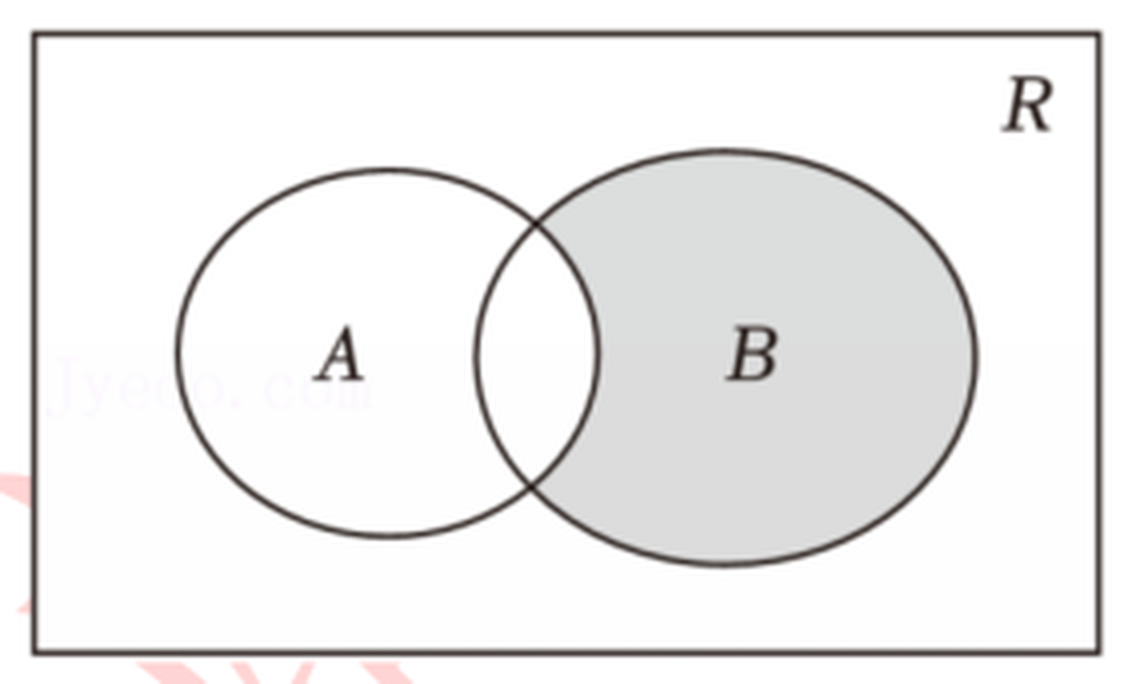
\includegraphics[width=0.30\textwidth]{figures/venn_Abar_cap_B.png}
\end{center}

\begin{enumerate}[label=(\arabic*)]
\item 若 $a=1$，求阴影部分表示的集合.
\item 若 $A\cap B=B$，求实数 $a$ 的取值范围.
\end{enumerate}

\ifanswer
\solbegin
\stepm{(1)}{因为 $\dfrac{2x-3}{x+5}\leqslant0$，
等价于 $\begin{cases}(2x-3)(x+5)\leqslant0\\ x+5\neq0\end{cases}$，}
\step{解得 $-5<x\leqslant\dfrac32$，即 $A=\left\{x\mid-5<x\leqslant\dfrac32\right\}$；}
\step{若 $a=1$，因为 $|x-1|<1$，等价于 $-1<x-1<1$，}
\step{解得 $0<x<2$，即 $B=\{x\mid0<x<2\}$.}
\step{由 Venn 图得阴影部分表示的集合为 $\overline{A}\cap B=\left(\dfrac32,2\right)$.}
\stepm{(2)}{由 (1) 得 $A=\left\{x\mid-5<x\leqslant\dfrac32\right\}$，}
\step{$B=\{x\mid|x-a|<1\}=\{x\mid-1+a<x<1+a\}\neq\varnothing$，}
\step{因为 $A\cap B=B$，所以 $B\sub A$，}
\step{所以 $\begin{cases}-5\leqslant-1+a\\ 1+a\leqslant\dfrac32\end{cases}$，
解得 $-4\leqslant a\leqslant\dfrac12$，}
\step{所以实数 $a$ 的取值范围为 $\left[-4,\dfrac12\right]$.}
\solend

\fi

\ansspace[6]

\item 设 $A=\{x\mid x^2-(m+3)x+2(m+1)=0,m\in\R\}$，
$B=\{x\mid 2x^2+(3n+1)x+2=0,n\in\R\}$.

\begin{enumerate}[label=(\arabic*)]
\item 是否存在 $m$、$n\in\R$，使得 $A=\{1,2\}$，$B=\varnothing$，说明理由；
\item 若 $A\cap B=A$，求 $m$、$n$ 的值.
\end{enumerate}

\ifanswer
\solbegin
\stepm{(1)}{由 $A=\{1,2\}$，得 $m=0$，}
\step{再由 $B=\varnothing$，得 $\Delta=(3n+1)^2-4\times2\times2=9n^2+6n-15<0$，}
\step{所以 $(3n+5)(n-1)<0$，解得 $-\dfrac53<n<1$，}
\step{故存在 $m=0$，$-\dfrac53<n<1$，使得 $A=\{1,2\}$，$B=\varnothing$.}
\stepm{(2)}{由 $x^2-(m+3)x+2(m+1)=0$，得 $x=2$ 或 $x=m+1$，}
\step{若 $A\cap B=A$，则 $A\sub B$，}
\step{将 $x=2$ 代入 $2x^2+(3n+1)x+2=0$，得 $n=-2$，}
\step{则 $B=\{x\mid 2x^2+(3n+1)x+2=0,n\in\R\}=\{x\mid 2x^2-5x+2=0\}
=\left\{2,\dfrac12\right\}$.}
\step{则 $m+1=\dfrac12$ 或 $m+1=2$，则 $m=-\dfrac12$ 或 $m=1$，
所以 $m=-\dfrac12$ 或 $m=1$，$n=-2$.}
\solend

\fi

\ansspace[6]

\item 已知陈述句 $\alpha$：关于 $x$ 的方程 $x^2-6x+m=0$ 有两个不同的正数根，陈述句
$\beta$：集合 $\{x\mid(m+1)x^2+4x+1=0,x\in\R\}$ 中至多有一个元素.

\begin{enumerate}[label=(\arabic*)]
\item 若 $\alpha$ 和 $\beta$ 都是真命题，求实数 $m$ 的取值范围；
\item 若 $\alpha$ 和 $\beta$ 至多有一个是假命题，求实数 $m$ 的取值范围.
\end{enumerate}

\ifanswer
\solbegin
\stepm{(1)}{因为关于 $x$ 的方程 $x^2-6x+m=0$ 有两个不同的正数根，}
\step{则 $\begin{cases}36-4m>0\\ m>0\end{cases}$，解得 $0<m<9$，}
\step{集合 $\{x\mid(m+1)x^2+4x+1=0,x\in\R\}$ 中至多有一个元素，}
\step{则 $m=-1$ 或 $\begin{cases}m+1\neq0\\ 16-4(m+1)\leqslant0\end{cases}$，
解得 $m\geqslant3$，}
\step{$\alpha$ 和 $\beta$ 都是真命题，所以实数 $m$ 的取值范围为 $\{m\mid3\leqslant m<9\}$}
\stepm{(2)}{由 (1) 得当 $\alpha$ 为假命题时，$m\leqslant0$ 或 $m\geqslant9$，}
\step{当 $\beta$ 为假命题时，$m<3$ 且 $m\neq-1$，}
\step{所以 $\alpha$ 和 $\beta$ 均为假命题时，$m$ 的范围是 $m\leqslant0$ 且 $m\neq-1$，}
\step{$\alpha$ 和 $\beta$ 至多有一个是假命题时，实数 $m$ 的取值范围为
$\{m\mid m>0$ 或 $m=-1\}$.}
\solend

\fi

\ansspace[6]

\item 已知符号 $[x]$ 表示不大于 $x$ 的最大整数 $(x\in\R)$，例如：$[1.3]=1$，
$[2]=2$，$[-1.2]=-2$.

\begin{enumerate}[label=(\arabic*)]
\item 已知方程 $[x]=3$，求该方程的解集；
\item 设方程 $\bigl[|x|+|x-1|\bigr]=3$ 的解集为 $A$，
集合 $B=\{x\mid 2x^2-11kx+15k^2\geqslant0\}$，若 $A\cup B=\R$，求实数 $k$ 的取值范围；
\item 在 (2) 的条件下，集合 $C=\{x\mid x^2-ax+1-2a\leqslant0,a\in\R\}$，是否存在实数
$a$，$A\cap C=A$，若存在，请求出实数 $a$ 的取值范围；若不存在，请说明理由.
\end{enumerate}

\ifanswer
\solbegin
\stepm{(1)}{方程 $[x]=3$，则 $x\in[3,4)$，所以该方程的解集为 $[3,4)$；}
\stepm{(2)}{因为 $\bigl[|x|+|x-1|\bigr]=3$，所以 $3\leqslant|x|+|x-1|<4$，}
\step{由绝对值不等式的几何意义得 $A=\left(-\dfrac32,-1\right]\cup\left[2,\dfrac52\right)$，}
\step{又 $B=\{x\mid 2x^2-11kx+15k^2\geqslant0\}=\{x\mid(2x-5k)(x-k)\geqslant0\}$，}
\step{当 $k=0$ 时，$B=\{x\mid 2x^2\geqslant0\}=\R$，则 $A\cup B=\R$，符合题意；}
\step{当 $k>0$ 时，$B=\left(-\infty,\dfrac{5k}{2}\right]\cup[3k,+\infty)$，
若 $A\cup B=\R$，}
\step{则 $\begin{cases}\dfrac{5k}{2}\geqslant2\\[2pt] 3k\leqslant\dfrac52\end{cases}$，
解得 $k\in\left[\dfrac45,\dfrac56\right]$；}
\step{当 $k<0$ 时，$B=(-\infty,3k]\cup\left[\dfrac{5k}{2},+\infty\right)$，
若 $A\cup B=\R$，}
\step{则 $\begin{cases}\dfrac{5k}{2}\leqslant-1\\[2pt] 3k\geqslant-\dfrac32\end{cases}$，
解得 $k\in\left[-\dfrac12,-\dfrac25\right]$.}
\step{综上所述，实数 $k$ 的取值范围为
$\left[-\dfrac12,-\dfrac25\right]\cup\{0\}\cup\left[\dfrac45,\dfrac56\right]$；}
\stepm{(3)}{因为 $A\cap C=A$，则 $A\sub C$ 且
$A=\left(-\dfrac32,-1\right]\cup\left[2,\dfrac52\right)$，}
\step{设集合 $C$ 的解集为 $(x_1,x_2)(x_1<x_2)$，}
\step{则 $\begin{cases}x_1\leqslant-\dfrac32\\[2pt] x_2\geqslant\dfrac52\end{cases}$，}
\step{所以
$\begin{cases}\Delta=a^2-4(1-2a)>0\\[2pt]
f\!\left(-\dfrac32\right)=\dfrac94+\dfrac32a+1-2a\leqslant0\\[4pt]
f\!\left(\dfrac52\right)=\dfrac{25}{4}-\dfrac52a+1-2a\leqslant0\end{cases}$，
解得 $a\geqslant\dfrac{13}{2}$，}
\step{故实数 $a$ 的取值范围为 $\left[\dfrac{13}{2},+\infty\right)$.}
\solend

\fi

\ansspace[6]

\item 非空有限集合 $S$ 是由若干个正实数组成，集合 $S$ 的元素个数不少于 $2$ 个. 对于任意
$a,b\in S,a\neq b$，若数 $a^b$ 或 $b^a$ 中至少有一个属于 $S$，则称集合 $S$ 是“好集”；
否则，称集合 $S$ 是“坏集”.

\begin{enumerate}[label=(\arabic*)]
\item 判断 $A=\{1,3,9\}$ 和 $B=\left\{1,\dfrac12,\dfrac14,\dfrac1{16}\right\}$ 是“好集”
还是“坏集”，并简单说明理由；
\item 题设的有限集 $S$ 中，既有大于 $1$ 的元素，又有小于 $1$ 的元素，证明：集合 $S$ 是
“坏集”；
\item 若题设中的 $a^b$ 或 $b^a$ 都属于 $S$，则称集合 $S$ 为“超级好集”，写出一个
“超级好集”（无须证明）.
\end{enumerate}

\ifanswer
\solbegin
\stepm{(1)}{$A=\{1,3,9\}$，$3^9\notin A$，$9^3\notin A$，所以 $A$ 是“坏集”，}
\step{从 $B$ 集合中任意取两个数字都满足需求，所以 $B$ 是“好集”.}
\stepm{(2)}{假设 $a$ 是 $S$ 中小于 $1$ 的元素中的最小元素，}
\step{$b$ 是 $S$ 中大于 $1$ 的元素中的最小元素，则 $a^b<a^1=a$，}
\step{所以 $a$ 就不是 $S$ 中小于 $1$ 的元素中的最小元素，即 $a^b\notin S$，}
\step{同理 $1=b^0<b^a<b^1=b$，所以 $b$ 就不是 $S$ 中大于 $1$ 的元素中的最小元素，}
\step{即 $b^a\notin S$，所以集合 $S$ 是“坏集”；}
\stepm{(3)}{首先 $S=\{1,a\}$（$a\neq1$ 且 $a>0$）是“超级好集”，}
\step{假设 $0<a<1$，由 (2) 得，$S$ 中不可能有大于 $1$ 的元素，}
\step{假设 $S$ 中有除 $a$ 之外的元素 $b\in S$（$a\neq b,b<1$），}
\step{假设 $a$ 是 $S$ 中小于 $1$ 的元素中的最大元素，$a^b>a^1=a$，}
\step{所以 $a$ 不是最大元素，所以 $a^b\notin S$，所以 $b\notin S$；}
\step{假设 $a>1$，由 (2) 得 $S$ 中不可能有小于 $1$ 的元素，}
\step{假设 $S$ 中有除 $a$ 之外的元素 $b$（$b>1$ 且 $b\neq a$），}
\step{假设 $a$ 是 $S$ 中大于 $1$ 的元素中的最小元素，则 $a^b>a^1=a$，}
\step{所以 $a$ 不是最小元素，即不存在 $b>1$，使得 $b\in S$，即 $b\notin S$，}
\step{综上，$S=\{1,a\}$（$a\neq1$ 且 $a>0$）.}
\solend

\fi

\ansspace*[10]

\end{enumerate}

\end{document}
"
%
% 原始材料是微信公众号图文（公众号「魔都数学加油站」连载「27学年高一 25」，2026-09-21 发布，
% 原文标题「27学年高一25——2026-2027年上海市华师大二附中高一上周末作业3」），
% 正文为 10 张 PNG 页（1080×1527，各页同尺寸）。原文本身就是一份**讲评版**——
% 题目下方直接印出【解析】（本卷无单独的【答案】行，填空题答案都写在解析里）。
% 试题文字与解析均照原卷录入，未改内容。卷面的粉色斜水印「魔都数学加油站」属水印，未录入。
%
% 卷首标题：原卷印作「2026-2027 年华师大二附中高一上周末作业 3」（公众号标题里的「上海市」
% 三字卷面标题行没有，本稿照卷面），年份区间按全稿惯例排 en dash，前缀照原卷保留「年」。
%
% 与原卷的排版差异（均已在 README「说明」中交代）：
%   ① 原文自**第 3 题**起（第 1、2 题未在该文中发布），故本稿题号亦自 3 起；
%   ② 原卷本就印有「一、填空题」「二、选择题」「三、解答题」三节标题，本稿照原卷分节，
%      只把标题改排成全稿统一的「大节标题」样式；
%   ③ 原卷第 13 题的答案「D」直接印在题干末尾的括号内，第 14—16 题的括号空着、答案写在
%      解析末句「故选 C／B」里；填空题的答案也都嵌在解析里，本稿统一改为试卷版隐去、
%      答案版以 \ans{} 给出（选择题另附【解析】），使两版彻底分离；
%   ④ 补集符号原卷一律作**上横线**（$\overline{A}$、$\overline{A\cup B}$），与同校的
%      高一14 同例，本稿照录（不改为 $\complement_U A$ 写法）；
%   ⑤ 原卷的实数集 R 斜体与粗体混用（第 17 题题干「全集为 R」作粗体，第 5、14 题与
%      第 16 题解析的 $R$ 为斜体），本稿按全稿惯例统一写作 $\R$；
%   ⑥ 原卷填空的横线约两个字宽，本稿按全稿惯例统一排 \blankline[4.4em]；
%   ⑦ 原卷未印副标题，本稿按全稿惯例补出副标题「集合与常用逻辑用语」；
%   ⑧ 第 17 题的 Venn 图原卷印在题干右侧（第 6 页），本稿移至题干之后；
%      图取原卷截图、4× LANCZOS 放大（figures/venn_Abar_cap_B.png，
%      阴影为 $B$ 中不含 $A\cap B$ 的部分，即 $\overline{A}\cap B$）。
%
% 原卷存疑两处（均照抄原卷、未改，见源码中该处上方注释）：
%   ① 第 8 题【解析】第二段「当 $\Delta=a^2-16>0$ 时，方程 $x^2+ax+4=0$ 有两个相同的根
%      $x_1$、$x_2$」——$\Delta>0$ 应为「两个**不**相同的根」（其自己的后文就把 $x_1$、$x_2$
%      当作可以不同的两个根在讨论），显系笔误；
%   ② 第 11 题【解析】先写「偶数必是 $2^{11}\cdot3^m\cdot337^n$，$m$、$n\in\N^*$」，
%      下一行又写「$0\leqslant m\leqslant10$，$0\leqslant n\leqslant10$，共有 121 种情况」
%      ——按 $\N^*$ 应从 1 起（至多 $10\times10=100$ 种），与 121（$=11\times11$，含 0）
%      对不上，两处至少有一处笔误。

\documentclass[a4paper,11pt]{article}
\usepackage{common}

\begin{document}

\examtitlest[3]{2026--2027 年华师大二附中高一上周末作业 3}{集合与常用逻辑用语}

\bigsec{一、填空题}

\begin{enumerate}
\setcounter{enumi}{2}

\item 设全集 $U=\{2,4,m^2+m-5\}$，集合 $A=\{2,1-m\}$，若 $\overline{A}=\{1\}$，则实数
$m=$ \blankline[4.4em].

\ifanswer
\solbegin
\step{因为 $\overline{A}=\{1\}$，所以 $1\in U$，$1\notin A$，}
\step{所以 $\begin{cases}m^2+m-5=1\\ 1-m\neq1\\ 1-m=4\end{cases}$，解得 $m=-3$.}
\solend

\fi

\item 已知条件 $\alpha$：$m<x\leqslant2m+5$，条件 $\beta$：$0\leqslant x\leqslant1$，
若 $\alpha$ 是 $\beta$ 的必要条件，则实数 $m$ 的取值范围为 \blankline[4.4em].

\ifanswer
\solbegin
\step{若 $\alpha$ 是 $\beta$ 的必要条件，则 $[0,1]\sub(m,2m+5]$，}
\step{所以 $\begin{cases}m<2m+5\\ m<0\\ 2m+5\geqslant1\end{cases}$，}
\step{解得 $-2\leqslant m<0$，故实数 $m$ 的取值范围为 $[-2,0)$.}
\solend

\fi

\item 已知 $\R$ 是全集，集合 $A=\{y\mid y=-x^2+1,x\in\R\}$，集合
$B=\{x\mid x=3+|a|,a\in\R\}$，则 $\overline{A\cup B}=$ \blankline[4.4em].

\ifanswer
\solbegin
\step{$A=\{y\mid y=-x^2+1,x\in\R\}=(-\infty,1]$，}
\step{$B=\{x\mid x=3+|a|,a\in\R\}=[3,+\infty)$，}
\step{所以 $\overline{A\cup B}=(1,3)$.}
\solend

\fi

\item 已知 $a$ 为常数，集合 $A=\{x\mid x^2+x-6=0\}$，集合 $B=\{x\mid ax-2=0\}$，且
$B\sub A$，则 $a$ 的所有取值构成的集合为 \blankline[4.4em].

\ifanswer
\solbegin
\step{集合 $A=\{-3,2\}$，因为 $B\sub A$，所以 $B=\varnothing$，$\{-3\}$，$\{2\}$，$\{-3,2\}$，}
\step{当 $B=\varnothing$ 时，$a=0$，当 $B=\{-3\}$ 时，$a=-\dfrac23$，当 $B=\{2\}$ 时，$a=1$，}
\step{当 $B=\{-3,2\}$ 时，不成立，故 $a$ 的取值集合为 $\left\{0,-\dfrac23,1\right\}$.}
\solend

\fi

\item 已知一元二次方程 $x^2+px+p=0$ 有两个不相等的实根分别为 $x_1$、$x_2$.
$A=x_1^2+x_2^2$，$B=x_1x_2(x_1+x_2)$，$A$ 与 $B$ 的大小为 \blankline[4.4em].

\ifanswer
\solbegin
\step{一元二次方程 $x^2+px+p=0$ 有两个不相等的实根分别为 $x_1$、$x_2$，}
\step{则 $\Delta=p^2-4p>0$，解得 $p<0$ 或 $p>4$，}
\step{由韦达定理得 $x_1+x_2=-p$，$x_1x_2=p$，}
\step{所以 $A=x_1^2+x_2^2=(x_1+x_2)^2-2x_1x_2=p^2-2p$，$B=x_1x_2(x_1+x_2)=-p^2$，}
\step{所以 $A-B=(p^2-2p)-(-p^2)=2p(p-1)$，}
\step{当 $p<0$ 时，则 $A-B>0$，故 $A>B$，}
\step{当 $p>4$ 时，则 $A-B>0$，故 $A>B$，}
\step{综上，$A=p^2-2p$，$B=-p^2$，且 $A>B$.}
\solend

\fi

\item 集合 $A=\{x\mid(x-1)(x^2+ax+4)=0,x\in\R\}$ 中所有元素之和为 $3$，则实数
$a=$ \blankline[4.4em].

\ifanswer
\solbegin
\step{当 $\Delta=a^2-16=0$ 时，方程 $x^2+ax+4=0$ 有两个相同的根 $-\dfrac a2$，}
\step{则 $A=\left\{1,-\dfrac a2\right\}$，故 $1-\dfrac a2=3$，解得 $a=-4$；}
% 注：下一行的「两个相同的根」系原卷笔误（△>0 应为「两个不相同的根」，其自己的后文
%     就把 x₁、x₂ 当作可以不同的两个根在讨论），照抄原卷、未改，见文件头「原卷存疑」①。
\step{当 $\Delta=a^2-16>0$ 时，方程 $x^2+ax+4=0$ 有两个相同的根 $x_1$、$x_2$，}
\step{若 $1$ 是方程 $x^2+ax+4=0$ 的根，则方程 $x^2+ax+4=0$ 的另一个根为 $4$，}
\step{则 $A=\{1,4\}$，不成立；}
\step{若 $1$ 不是方程 $x^2+ax+4=0$ 的根，则 $A=\{1,x_1,x_2\}$，则 $1+x_1+x_2=3$，}
\step{故 $x_1+x_2=2=-a$，故 $a=-2$（舍去）；}
\step{综上所述，$a=-4$.}
\solend

\fi

\item 已知集合 $A=\{x\mid x^2+2x-8\geqslant0\}$，$B=\{x\mid x^2-2ax+4\leqslant0\}$，
若 $a>0$，且 $A\cap B\cap\N$ 中恰有 $2$ 个元素，则 $a$ 的取值范围为 \blankline[4.4em].

\ifanswer
\solbegin
\step{由 $A$ 中不等式变形得 $(x-2)(x+4)\geqslant0$，解得 $x\leqslant-4$ 或 $x\geqslant2$，}
\step{即 $A=(-\infty,-4]\cup[2,+\infty)$，}
\step{设 $f(x)=x^2-2ax+4$，则 $f(x)$ 的轴对称 $x=a>0$，}
\step{且对应方程的根 $x_1$、$x_2$ 满足 $\begin{cases}x_1x_2=4\\ x_1+x_2>0\end{cases}$，}
\step{所以 $0<x_1\leqslant2\leqslant x_2$（取 $x_1\leqslant x_2$），}
\step{所以 $A\cap B\cap\N$ 中恰有的整数为 $2$，$3$，}
\step{所以 $\begin{cases}f(3)=9-6a+4\leqslant0\\ f(4)=16-8a+4>0\end{cases}$，}
\step{解得 $\dfrac{13}{6}\leqslant a<\dfrac52$，所以 $a$ 的取值范围为 $\left[\dfrac{13}{6},\dfrac52\right)$.}
\solend

\fi

\item 在三个关于 $x$ 的方程 $x^2-ax+4=0$，$x^2+(a-1)x+16=0$ 和
$x^2+2ax+3a+10=0$ 中至少有一个方程有实根，则实数 $a$ 的取值范围是 \blankline[4.4em].

\ifanswer
\solbegin
\step{当三个方程均无实根时，有}
\step{$\begin{cases}\Delta_1=a^2-16<0\\ \Delta_2=(a-1)^2-64<0\\ \Delta_3=4a^2-4(3a+10)<0\end{cases}$，}
\step{所以 $\begin{cases}-4<a<4\\ -7<a<9\\ -2<a<5\end{cases}$，}
\step{所以 $-2<a<4$，故三个方程均无实根时，$a$ 的取值范围为 $(-2,4)$，}
\step{所以三个方程中至少有一个方程有实根时，}
\step{实数 $a$ 的取值范围为 $(-\infty,-2]\cup[4,+\infty)$.}
\solend

\fi

% 注：下一行解析里的「m、n∈N*」与再下一行的「0≤m≤10，0≤n≤10，共有 121 种情况」
%     对不上（按 N* 应从 1 起，至多 10×10=100 种；121=11×11 含 0），系原卷自身矛盾，
%     照抄原卷、未改，见文件头「原卷存疑」②。
\item 若集合 $M=\{(x,y)\mid(x+1)+(x+2)+\cdots+(x+y)=2022^{10},x\in\Z,y\in\N^{*}\}$，
则集合 $M$ 中元素有 \blankline[4.4em] 个.

\ifanswer
\solbegin
\step{由题意得 $(x+1)+(x+2)+\cdots+(x+y)=\dfrac{y(2x+1+y)}{2}$，}
\step{所以 $y(2x+1+y)=2^{11}\cdot3^{10}\cdot337^{10}$，}
\step{因为 $y$ 与 $2x+1+y$ 必为一奇一偶，偶数必是 $2^{11}\cdot3^m\cdot337^n$，
$m$、$n\in\N^{*}$，}
\step{$0\leqslant m\leqslant10$，$0\leqslant n\leqslant10$，共有 $121$ 种情况，}
\step{因为 $y$ 与 $2x+1+y$ 奇偶未定，所以集合 $M$ 中元素只有 $242$ 个.}
\solend

\fi

\item 设集合 $M=\left\{x\mid m\leqslant x\leqslant m+\dfrac34\right\}$，
$N=\left\{x\mid n-\dfrac13\leqslant x\leqslant n\right\}$，且 $M$、$N$ 都是集合
$\{x\mid0\leqslant x\leqslant1\}$ 的子集，如果把 $b-a$ 叫做集合
$\{x\mid a\leqslant x\leqslant b\}$ 的长度，那么集合 $M\cap N$ 的长度的最小值是
\blankline[4.4em].

\ifanswer
\solbegin
\step{$M$ 的长度为 $\dfrac34$，$N$ 的长度为 $\dfrac13$，}
\step{当集合 $M\cap N$ 的长度的最小值时，$M$ 与 $N$ 应分别在区间 $[0,1]$ 的左右两端，}
\step{故 $M\cap N$ 的长度的最小值是 $\dfrac34+\dfrac13-1=\dfrac1{12}$.}
\solend

\fi

\end{enumerate}

\bigsec{二、选择题}

\begin{enumerate}
\setcounter{enumi}{12}

\item 直角坐标平面中除去两点 $A(1,1)$、$B(2,-2)$ 可用集合表示为\mbox{（\quad）}

\keepwithprev
A. $\{(x,y)\mid x\neq1,y\neq1,x\neq2,y\neq-2$\}\qquad
B. $\{(x,y)\mid\begin{cases}x\neq1\\ y\neq1\end{cases}$ 或 $\begin{cases}x\neq2\\ y\neq-2\end{cases}\}$

C. $\{(x,y)\mid[(x-1)^2+(y-1)^2][(x-2)^2+(y+2)^2]\neq0$\}

D. $\{(x,y)\mid[(x-1)^2+(y-1)^2]+[(x-2)^2+(y+2)^2]\neq0$\}

\ans{$D$}

\item 已知函数 $f(x)=x^2+nx$，记集合 $A=\{x\mid f(x)=0,x\in\R\}$，
$B=\{x\mid f(f(x))=0,x\in\R\}$，若 $A=B\neq\varnothing$，则 $n$ 的取值范围是\mbox{（\quad）}

\keepwithprev
A. $[0,4]$\qquad B. $(0,4)$\qquad C. $[0,4)$\qquad D. $(0,4]$

\ans{$C$}

\ifanswer
\solbegin
\step{$f(x)=x^2+nx$，$f[f(x)]=(x^2+nx)^2+n(x^2+nx)=(x^2+nx)(x^2+nx+n)$，}
\step{当 $n=0$ 时，$f(x)=x^2$，$f[f(x)]=x^4$，满足 $A=B$，此时 $n=0$；}
\step{当 $n\neq0$ 时，$0$、$-n$ 不是 $x^2+nx+n=0$ 的根，故 $\Delta=n^2-4n<0$，
解得 $0<n<4$，}
\step{综上所述，$n$ 的取值范围是 $[0,4)$. 故选 $C$.}
\solend

\fi

\item 设全集 $U=\{1,2,3,4,5,6,7,8,9,10\}$，给出条件：① $A\sub U$；②若 $x\in A$，
则 $2x\notin A$；③若 $x\in\overline{A}$，则 $2x\notin\overline{A}$.
那么同时满足三个条件的集合 $A$ 的个数为\mbox{（\quad）}

\keepwithprev
A. $0$ 个\qquad B. $16$ 个\qquad C. $32$ 个\qquad D. $64$ 个

\ans{$C$}

\ifanswer
\solbegin
\step{由① $A\sub U$；②若 $x\in A$，则 $2x\notin A$；③若 $x\in\overline{A}$，
则 $2x\notin\overline{A}$.}
\step{若 $1\in A$，则 $2\notin A$，即 $2\in\overline{A}$，则 $4\notin\overline{A}$，
即 $4\in A$，则 $8\notin A$，即 $8\in\overline{A}$；}
\step{若 $3\in A$，则 $6\notin A$，即 $6\in\overline{A}$；若 $5\in A$，则 $10\notin A$，
即 $10\in\overline{A}$，}
\step{故 $1$、$4$ 和 $2$、$8$ 分开，$3$ 和 $6$ 分开，$5$ 和 $10$ 分开，$7$ 和 $9$ 随意，}
\step{故同时满足三个条件的集合 $A$ 的个数为 $2\times2\times2\times2\times2=32$，
故选 $C$.}
\solend

\fi

\item 设集合 $P_1=\{x\mid x^2+ax+1>0\}$，$P_2=\{x\mid x^2+ax+2>0\}$，
$Q_1=\{x\mid x^2+x+b>0\}$，$Q_2=\{x\mid x^2+2x+b>0\}$，其中 $a$、$b\in\R$，
下列说法中正确的是\mbox{（\quad）}

\keepwithprev
A. 对任意 $a$，$P_1$ 是 $P_2$ 的子集，对任意的 $b$，$Q_1$ 不是 $Q_2$ 的子集

B. 对任意 $a$，$P_1$ 是 $P_2$ 的子集，存在 $b$，使得 $Q_1$ 是 $Q_2$ 的子集

C. 存在 $a$，使得 $P_1$ 不是 $P_2$ 的子集，对任意的 $b$，$Q_1$ 不是 $Q_2$ 的子集

D. 存在 $a$，使得 $P_1$ 不是 $P_2$ 的子集，存在 $b$，使得 $Q_1$ 是 $Q_2$ 的子集

\ans{$B$}

\ifanswer
\solbegin
\step{对于集合 $P_1=\{x\mid x^2+ax+1>0\}$，$P_2=\{x\mid x^2+ax+2>0\}$，}
\step{得当 $m\in P_1$ 时，即 $m^2+am+1>0$，得 $m^2+am+2>0$，}
\step{即有 $m\in P_2$，得对任意 $a$，$P_1$ 是 $P_2$ 的子集，}
\step{对于集合 $Q_1=\{x\mid x^2+x+b>0\}$，$Q_2=\{x\mid x^2+2x+b>0\}$，}
\step{当 $b=6$ 时，$Q_1=\{x\mid x^2+x+6>0\}=\R$，$Q_2=\{x\mid x^2+2x+6>0\}=\R$，}
\step{得 $Q_1$ 是 $Q_2$ 的子集，}
\step{当 $b=1$ 时，$Q_1=\{x\mid x^2+x+1>0\}=\R$，}
\step{$Q_2=\{x\mid x^2+2x+1>0\}=\{x\mid x\neq-1\}$，得 $Q_1$ 不是 $Q_2$ 的子集，}
\step{所以存在 $b$，使得 $Q_1$ 是 $Q_2$ 的子集，故选 $B$.}
\solend

\fi

\end{enumerate}

\bigsec{三、解答题}

\begin{enumerate}
\setcounter{enumi}{16}

\item 已知集合 $A=\left\{x\mid\dfrac{2x-3}{x+5}\leqslant0\right\}$，
$B=\{x\mid|x-a|<1\}$，全集为 $\R$.

\begin{center}
% 图取原卷截图、4× LANCZOS 放大（原卷把图印在题干右侧，本稿移至此处，见文件头⑧）。
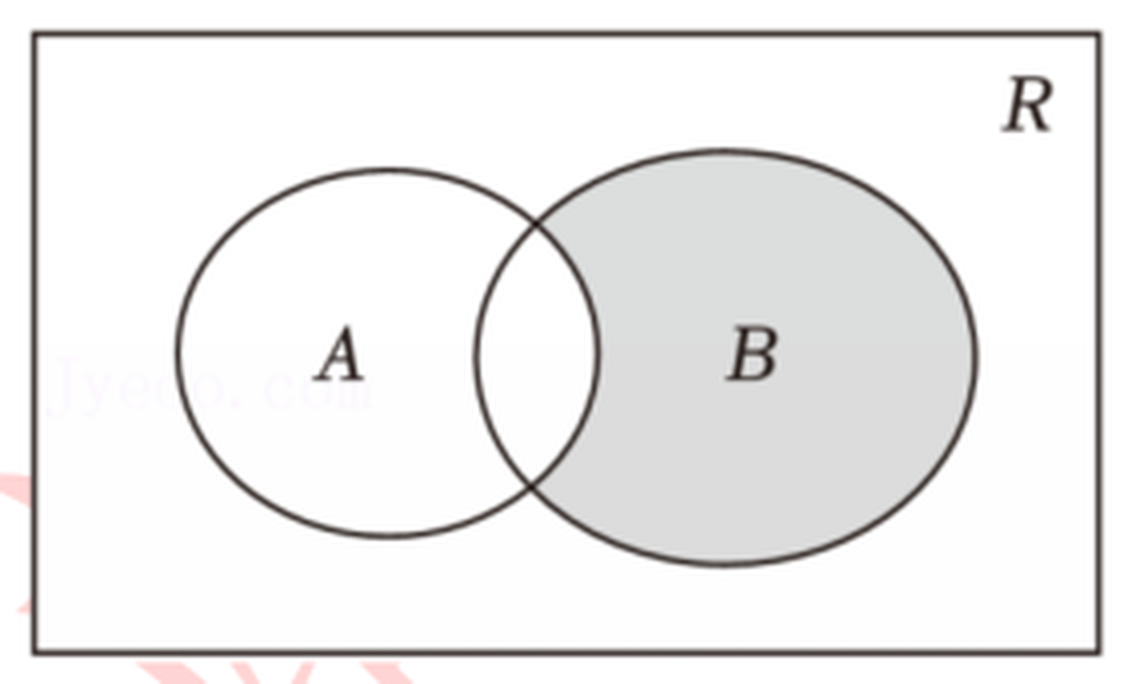
\includegraphics[width=0.30\textwidth]{figures/venn_Abar_cap_B.png}
\end{center}

\begin{enumerate}[label=(\arabic*)]
\item 若 $a=1$，求阴影部分表示的集合.
\item 若 $A\cap B=B$，求实数 $a$ 的取值范围.
\end{enumerate}

\ifanswer
\solbegin
\stepm{(1)}{因为 $\dfrac{2x-3}{x+5}\leqslant0$，
等价于 $\begin{cases}(2x-3)(x+5)\leqslant0\\ x+5\neq0\end{cases}$，}
\step{解得 $-5<x\leqslant\dfrac32$，即 $A=\left\{x\mid-5<x\leqslant\dfrac32\right\}$；}
\step{若 $a=1$，因为 $|x-1|<1$，等价于 $-1<x-1<1$，}
\step{解得 $0<x<2$，即 $B=\{x\mid0<x<2\}$.}
\step{由 Venn 图得阴影部分表示的集合为 $\overline{A}\cap B=\left(\dfrac32,2\right)$.}
\stepm{(2)}{由 (1) 得 $A=\left\{x\mid-5<x\leqslant\dfrac32\right\}$，}
\step{$B=\{x\mid|x-a|<1\}=\{x\mid-1+a<x<1+a\}\neq\varnothing$，}
\step{因为 $A\cap B=B$，所以 $B\sub A$，}
\step{所以 $\begin{cases}-5\leqslant-1+a\\ 1+a\leqslant\dfrac32\end{cases}$，
解得 $-4\leqslant a\leqslant\dfrac12$，}
\step{所以实数 $a$ 的取值范围为 $\left[-4,\dfrac12\right]$.}
\solend

\fi

\ansspace[6]

\item 设 $A=\{x\mid x^2-(m+3)x+2(m+1)=0,m\in\R\}$，
$B=\{x\mid 2x^2+(3n+1)x+2=0,n\in\R\}$.

\begin{enumerate}[label=(\arabic*)]
\item 是否存在 $m$、$n\in\R$，使得 $A=\{1,2\}$，$B=\varnothing$，说明理由；
\item 若 $A\cap B=A$，求 $m$、$n$ 的值.
\end{enumerate}

\ifanswer
\solbegin
\stepm{(1)}{由 $A=\{1,2\}$，得 $m=0$，}
\step{再由 $B=\varnothing$，得 $\Delta=(3n+1)^2-4\times2\times2=9n^2+6n-15<0$，}
\step{所以 $(3n+5)(n-1)<0$，解得 $-\dfrac53<n<1$，}
\step{故存在 $m=0$，$-\dfrac53<n<1$，使得 $A=\{1,2\}$，$B=\varnothing$.}
\stepm{(2)}{由 $x^2-(m+3)x+2(m+1)=0$，得 $x=2$ 或 $x=m+1$，}
\step{若 $A\cap B=A$，则 $A\sub B$，}
\step{将 $x=2$ 代入 $2x^2+(3n+1)x+2=0$，得 $n=-2$，}
\step{则 $B=\{x\mid 2x^2+(3n+1)x+2=0,n\in\R\}=\{x\mid 2x^2-5x+2=0\}
=\left\{2,\dfrac12\right\}$.}
\step{则 $m+1=\dfrac12$ 或 $m+1=2$，则 $m=-\dfrac12$ 或 $m=1$，
所以 $m=-\dfrac12$ 或 $m=1$，$n=-2$.}
\solend

\fi

\ansspace[6]

\item 已知陈述句 $\alpha$：关于 $x$ 的方程 $x^2-6x+m=0$ 有两个不同的正数根，陈述句
$\beta$：集合 $\{x\mid(m+1)x^2+4x+1=0,x\in\R\}$ 中至多有一个元素.

\begin{enumerate}[label=(\arabic*)]
\item 若 $\alpha$ 和 $\beta$ 都是真命题，求实数 $m$ 的取值范围；
\item 若 $\alpha$ 和 $\beta$ 至多有一个是假命题，求实数 $m$ 的取值范围.
\end{enumerate}

\ifanswer
\solbegin
\stepm{(1)}{因为关于 $x$ 的方程 $x^2-6x+m=0$ 有两个不同的正数根，}
\step{则 $\begin{cases}36-4m>0\\ m>0\end{cases}$，解得 $0<m<9$，}
\step{集合 $\{x\mid(m+1)x^2+4x+1=0,x\in\R\}$ 中至多有一个元素，}
\step{则 $m=-1$ 或 $\begin{cases}m+1\neq0\\ 16-4(m+1)\leqslant0\end{cases}$，
解得 $m\geqslant3$，}
\step{$\alpha$ 和 $\beta$ 都是真命题，所以实数 $m$ 的取值范围为 $\{m\mid3\leqslant m<9\}$}
\stepm{(2)}{由 (1) 得当 $\alpha$ 为假命题时，$m\leqslant0$ 或 $m\geqslant9$，}
\step{当 $\beta$ 为假命题时，$m<3$ 且 $m\neq-1$，}
\step{所以 $\alpha$ 和 $\beta$ 均为假命题时，$m$ 的范围是 $m\leqslant0$ 且 $m\neq-1$，}
\step{$\alpha$ 和 $\beta$ 至多有一个是假命题时，实数 $m$ 的取值范围为
$\{m\mid m>0$ 或 $m=-1\}$.}
\solend

\fi

\ansspace[6]

\item 已知符号 $[x]$ 表示不大于 $x$ 的最大整数 $(x\in\R)$，例如：$[1.3]=1$，
$[2]=2$，$[-1.2]=-2$.

\begin{enumerate}[label=(\arabic*)]
\item 已知方程 $[x]=3$，求该方程的解集；
\item 设方程 $\bigl[|x|+|x-1|\bigr]=3$ 的解集为 $A$，
集合 $B=\{x\mid 2x^2-11kx+15k^2\geqslant0\}$，若 $A\cup B=\R$，求实数 $k$ 的取值范围；
\item 在 (2) 的条件下，集合 $C=\{x\mid x^2-ax+1-2a\leqslant0,a\in\R\}$，是否存在实数
$a$，$A\cap C=A$，若存在，请求出实数 $a$ 的取值范围；若不存在，请说明理由.
\end{enumerate}

\ifanswer
\solbegin
\stepm{(1)}{方程 $[x]=3$，则 $x\in[3,4)$，所以该方程的解集为 $[3,4)$；}
\stepm{(2)}{因为 $\bigl[|x|+|x-1|\bigr]=3$，所以 $3\leqslant|x|+|x-1|<4$，}
\step{由绝对值不等式的几何意义得 $A=\left(-\dfrac32,-1\right]\cup\left[2,\dfrac52\right)$，}
\step{又 $B=\{x\mid 2x^2-11kx+15k^2\geqslant0\}=\{x\mid(2x-5k)(x-k)\geqslant0\}$，}
\step{当 $k=0$ 时，$B=\{x\mid 2x^2\geqslant0\}=\R$，则 $A\cup B=\R$，符合题意；}
\step{当 $k>0$ 时，$B=\left(-\infty,\dfrac{5k}{2}\right]\cup[3k,+\infty)$，
若 $A\cup B=\R$，}
\step{则 $\begin{cases}\dfrac{5k}{2}\geqslant2\\[2pt] 3k\leqslant\dfrac52\end{cases}$，
解得 $k\in\left[\dfrac45,\dfrac56\right]$；}
\step{当 $k<0$ 时，$B=(-\infty,3k]\cup\left[\dfrac{5k}{2},+\infty\right)$，
若 $A\cup B=\R$，}
\step{则 $\begin{cases}\dfrac{5k}{2}\leqslant-1\\[2pt] 3k\geqslant-\dfrac32\end{cases}$，
解得 $k\in\left[-\dfrac12,-\dfrac25\right]$.}
\step{综上所述，实数 $k$ 的取值范围为
$\left[-\dfrac12,-\dfrac25\right]\cup\{0\}\cup\left[\dfrac45,\dfrac56\right]$；}
\stepm{(3)}{因为 $A\cap C=A$，则 $A\sub C$ 且
$A=\left(-\dfrac32,-1\right]\cup\left[2,\dfrac52\right)$，}
\step{设集合 $C$ 的解集为 $(x_1,x_2)(x_1<x_2)$，}
\step{则 $\begin{cases}x_1\leqslant-\dfrac32\\[2pt] x_2\geqslant\dfrac52\end{cases}$，}
\step{所以
$\begin{cases}\Delta=a^2-4(1-2a)>0\\[2pt]
f\!\left(-\dfrac32\right)=\dfrac94+\dfrac32a+1-2a\leqslant0\\[4pt]
f\!\left(\dfrac52\right)=\dfrac{25}{4}-\dfrac52a+1-2a\leqslant0\end{cases}$，
解得 $a\geqslant\dfrac{13}{2}$，}
\step{故实数 $a$ 的取值范围为 $\left[\dfrac{13}{2},+\infty\right)$.}
\solend

\fi

\ansspace[6]

\item 非空有限集合 $S$ 是由若干个正实数组成，集合 $S$ 的元素个数不少于 $2$ 个. 对于任意
$a,b\in S,a\neq b$，若数 $a^b$ 或 $b^a$ 中至少有一个属于 $S$，则称集合 $S$ 是“好集”；
否则，称集合 $S$ 是“坏集”.

\begin{enumerate}[label=(\arabic*)]
\item 判断 $A=\{1,3,9\}$ 和 $B=\left\{1,\dfrac12,\dfrac14,\dfrac1{16}\right\}$ 是“好集”
还是“坏集”，并简单说明理由；
\item 题设的有限集 $S$ 中，既有大于 $1$ 的元素，又有小于 $1$ 的元素，证明：集合 $S$ 是
“坏集”；
\item 若题设中的 $a^b$ 或 $b^a$ 都属于 $S$，则称集合 $S$ 为“超级好集”，写出一个
“超级好集”（无须证明）.
\end{enumerate}

\ifanswer
\solbegin
\stepm{(1)}{$A=\{1,3,9\}$，$3^9\notin A$，$9^3\notin A$，所以 $A$ 是“坏集”，}
\step{从 $B$ 集合中任意取两个数字都满足需求，所以 $B$ 是“好集”.}
\stepm{(2)}{假设 $a$ 是 $S$ 中小于 $1$ 的元素中的最小元素，}
\step{$b$ 是 $S$ 中大于 $1$ 的元素中的最小元素，则 $a^b<a^1=a$，}
\step{所以 $a$ 就不是 $S$ 中小于 $1$ 的元素中的最小元素，即 $a^b\notin S$，}
\step{同理 $1=b^0<b^a<b^1=b$，所以 $b$ 就不是 $S$ 中大于 $1$ 的元素中的最小元素，}
\step{即 $b^a\notin S$，所以集合 $S$ 是“坏集”；}
\stepm{(3)}{首先 $S=\{1,a\}$（$a\neq1$ 且 $a>0$）是“超级好集”，}
\step{假设 $0<a<1$，由 (2) 得，$S$ 中不可能有大于 $1$ 的元素，}
\step{假设 $S$ 中有除 $a$ 之外的元素 $b\in S$（$a\neq b,b<1$），}
\step{假设 $a$ 是 $S$ 中小于 $1$ 的元素中的最大元素，$a^b>a^1=a$，}
\step{所以 $a$ 不是最大元素，所以 $a^b\notin S$，所以 $b\notin S$；}
\step{假设 $a>1$，由 (2) 得 $S$ 中不可能有小于 $1$ 的元素，}
\step{假设 $S$ 中有除 $a$ 之外的元素 $b$（$b>1$ 且 $b\neq a$），}
\step{假设 $a$ 是 $S$ 中大于 $1$ 的元素中的最小元素，则 $a^b>a^1=a$，}
\step{所以 $a$ 不是最小元素，即不存在 $b>1$，使得 $b\in S$，即 $b\notin S$，}
\step{综上，$S=\{1,a\}$（$a\neq1$ 且 $a>0$）.}
\solend

\fi

\ansspace*[10]

\end{enumerate}

\end{document}
"
%
% 原始材料是微信公众号图文（公众号「魔都数学加油站」连载「27学年高一 25」，2026-09-21 发布，
% 原文标题「27学年高一25——2026-2027年上海市华师大二附中高一上周末作业3」），
% 正文为 10 张 PNG 页（1080×1527，各页同尺寸）。原文本身就是一份**讲评版**——
% 题目下方直接印出【解析】（本卷无单独的【答案】行，填空题答案都写在解析里）。
% 试题文字与解析均照原卷录入，未改内容。卷面的粉色斜水印「魔都数学加油站」属水印，未录入。
%
% 卷首标题：原卷印作「2026-2027 年华师大二附中高一上周末作业 3」（公众号标题里的「上海市」
% 三字卷面标题行没有，本稿照卷面），年份区间按全稿惯例排 en dash，前缀照原卷保留「年」。
%
% 与原卷的排版差异（均已在 README「说明」中交代）：
%   ① 原文自**第 3 题**起（第 1、2 题未在该文中发布），故本稿题号亦自 3 起；
%   ② 原卷本就印有「一、填空题」「二、选择题」「三、解答题」三节标题，本稿照原卷分节，
%      只把标题改排成全稿统一的「大节标题」样式；
%   ③ 原卷第 13 题的答案「D」直接印在题干末尾的括号内，第 14—16 题的括号空着、答案写在
%      解析末句「故选 C／B」里；填空题的答案也都嵌在解析里，本稿统一改为试卷版隐去、
%      答案版以 \ans{} 给出（选择题另附【解析】），使两版彻底分离；
%   ④ 补集符号原卷一律作**上横线**（$\overline{A}$、$\overline{A\cup B}$），与同校的
%      高一14 同例，本稿照录（不改为 $\complement_U A$ 写法）；
%   ⑤ 原卷的实数集 R 斜体与粗体混用（第 17 题题干「全集为 R」作粗体，第 5、14 题与
%      第 16 题解析的 $R$ 为斜体），本稿按全稿惯例统一写作 $\R$；
%   ⑥ 原卷填空的横线约两个字宽，本稿按全稿惯例统一排 \blankline[4.4em]；
%   ⑦ 原卷未印副标题，本稿按全稿惯例补出副标题「集合与常用逻辑用语」；
%   ⑧ 第 17 题的 Venn 图原卷印在题干右侧（第 6 页），本稿移至题干之后；
%      图取原卷截图、4× LANCZOS 放大（figures/venn_Abar_cap_B.png，
%      阴影为 $B$ 中不含 $A\cap B$ 的部分，即 $\overline{A}\cap B$）。
%
% 原卷存疑两处（均照抄原卷、未改，见源码中该处上方注释）：
%   ① 第 8 题【解析】第二段「当 $\Delta=a^2-16>0$ 时，方程 $x^2+ax+4=0$ 有两个相同的根
%      $x_1$、$x_2$」——$\Delta>0$ 应为「两个**不**相同的根」（其自己的后文就把 $x_1$、$x_2$
%      当作可以不同的两个根在讨论），显系笔误；
%   ② 第 11 题【解析】先写「偶数必是 $2^{11}\cdot3^m\cdot337^n$，$m$、$n\in\N^*$」，
%      下一行又写「$0\leqslant m\leqslant10$，$0\leqslant n\leqslant10$，共有 121 种情况」
%      ——按 $\N^*$ 应从 1 起（至多 $10\times10=100$ 种），与 121（$=11\times11$，含 0）
%      对不上，两处至少有一处笔误。

\documentclass[a4paper,11pt]{article}
\usepackage{common}

\begin{document}

\examtitlest[3]{2026--2027 年华师大二附中高一上周末作业 3}{集合与常用逻辑用语}

\bigsec{一、填空题}

\begin{enumerate}
\setcounter{enumi}{2}

\item 设全集 $U=\{2,4,m^2+m-5\}$，集合 $A=\{2,1-m\}$，若 $\overline{A}=\{1\}$，则实数
$m=$ \blankline[4.4em].

\ifanswer
\solbegin
\step{因为 $\overline{A}=\{1\}$，所以 $1\in U$，$1\notin A$，}
\step{所以 $\begin{cases}m^2+m-5=1\\ 1-m\neq1\\ 1-m=4\end{cases}$，解得 $m=-3$.}
\solend

\fi

\item 已知条件 $\alpha$：$m<x\leqslant2m+5$，条件 $\beta$：$0\leqslant x\leqslant1$，
若 $\alpha$ 是 $\beta$ 的必要条件，则实数 $m$ 的取值范围为 \blankline[4.4em].

\ifanswer
\solbegin
\step{若 $\alpha$ 是 $\beta$ 的必要条件，则 $[0,1]\sub(m,2m+5]$，}
\step{所以 $\begin{cases}m<2m+5\\ m<0\\ 2m+5\geqslant1\end{cases}$，}
\step{解得 $-2\leqslant m<0$，故实数 $m$ 的取值范围为 $[-2,0)$.}
\solend

\fi

\item 已知 $\R$ 是全集，集合 $A=\{y\mid y=-x^2+1,x\in\R\}$，集合
$B=\{x\mid x=3+|a|,a\in\R\}$，则 $\overline{A\cup B}=$ \blankline[4.4em].

\ifanswer
\solbegin
\step{$A=\{y\mid y=-x^2+1,x\in\R\}=(-\infty,1]$，}
\step{$B=\{x\mid x=3+|a|,a\in\R\}=[3,+\infty)$，}
\step{所以 $\overline{A\cup B}=(1,3)$.}
\solend

\fi

\item 已知 $a$ 为常数，集合 $A=\{x\mid x^2+x-6=0\}$，集合 $B=\{x\mid ax-2=0\}$，且
$B\sub A$，则 $a$ 的所有取值构成的集合为 \blankline[4.4em].

\ifanswer
\solbegin
\step{集合 $A=\{-3,2\}$，因为 $B\sub A$，所以 $B=\varnothing$，$\{-3\}$，$\{2\}$，$\{-3,2\}$，}
\step{当 $B=\varnothing$ 时，$a=0$，当 $B=\{-3\}$ 时，$a=-\dfrac23$，当 $B=\{2\}$ 时，$a=1$，}
\step{当 $B=\{-3,2\}$ 时，不成立，故 $a$ 的取值集合为 $\left\{0,-\dfrac23,1\right\}$.}
\solend

\fi

\item 已知一元二次方程 $x^2+px+p=0$ 有两个不相等的实根分别为 $x_1$、$x_2$.
$A=x_1^2+x_2^2$，$B=x_1x_2(x_1+x_2)$，$A$ 与 $B$ 的大小为 \blankline[4.4em].

\ifanswer
\solbegin
\step{一元二次方程 $x^2+px+p=0$ 有两个不相等的实根分别为 $x_1$、$x_2$，}
\step{则 $\Delta=p^2-4p>0$，解得 $p<0$ 或 $p>4$，}
\step{由韦达定理得 $x_1+x_2=-p$，$x_1x_2=p$，}
\step{所以 $A=x_1^2+x_2^2=(x_1+x_2)^2-2x_1x_2=p^2-2p$，$B=x_1x_2(x_1+x_2)=-p^2$，}
\step{所以 $A-B=(p^2-2p)-(-p^2)=2p(p-1)$，}
\step{当 $p<0$ 时，则 $A-B>0$，故 $A>B$，}
\step{当 $p>4$ 时，则 $A-B>0$，故 $A>B$，}
\step{综上，$A=p^2-2p$，$B=-p^2$，且 $A>B$.}
\solend

\fi

\item 集合 $A=\{x\mid(x-1)(x^2+ax+4)=0,x\in\R\}$ 中所有元素之和为 $3$，则实数
$a=$ \blankline[4.4em].

\ifanswer
\solbegin
\step{当 $\Delta=a^2-16=0$ 时，方程 $x^2+ax+4=0$ 有两个相同的根 $-\dfrac a2$，}
\step{则 $A=\left\{1,-\dfrac a2\right\}$，故 $1-\dfrac a2=3$，解得 $a=-4$；}
% 注：下一行的「两个相同的根」系原卷笔误（△>0 应为「两个不相同的根」，其自己的后文
%     就把 x₁、x₂ 当作可以不同的两个根在讨论），照抄原卷、未改，见文件头「原卷存疑」①。
\step{当 $\Delta=a^2-16>0$ 时，方程 $x^2+ax+4=0$ 有两个相同的根 $x_1$、$x_2$，}
\step{若 $1$ 是方程 $x^2+ax+4=0$ 的根，则方程 $x^2+ax+4=0$ 的另一个根为 $4$，}
\step{则 $A=\{1,4\}$，不成立；}
\step{若 $1$ 不是方程 $x^2+ax+4=0$ 的根，则 $A=\{1,x_1,x_2\}$，则 $1+x_1+x_2=3$，}
\step{故 $x_1+x_2=2=-a$，故 $a=-2$（舍去）；}
\step{综上所述，$a=-4$.}
\solend

\fi

\item 已知集合 $A=\{x\mid x^2+2x-8\geqslant0\}$，$B=\{x\mid x^2-2ax+4\leqslant0\}$，
若 $a>0$，且 $A\cap B\cap\N$ 中恰有 $2$ 个元素，则 $a$ 的取值范围为 \blankline[4.4em].

\ifanswer
\solbegin
\step{由 $A$ 中不等式变形得 $(x-2)(x+4)\geqslant0$，解得 $x\leqslant-4$ 或 $x\geqslant2$，}
\step{即 $A=(-\infty,-4]\cup[2,+\infty)$，}
\step{设 $f(x)=x^2-2ax+4$，则 $f(x)$ 的轴对称 $x=a>0$，}
\step{且对应方程的根 $x_1$、$x_2$ 满足 $\begin{cases}x_1x_2=4\\ x_1+x_2>0\end{cases}$，}
\step{所以 $0<x_1\leqslant2\leqslant x_2$（取 $x_1\leqslant x_2$），}
\step{所以 $A\cap B\cap\N$ 中恰有的整数为 $2$，$3$，}
\step{所以 $\begin{cases}f(3)=9-6a+4\leqslant0\\ f(4)=16-8a+4>0\end{cases}$，}
\step{解得 $\dfrac{13}{6}\leqslant a<\dfrac52$，所以 $a$ 的取值范围为 $\left[\dfrac{13}{6},\dfrac52\right)$.}
\solend

\fi

\item 在三个关于 $x$ 的方程 $x^2-ax+4=0$，$x^2+(a-1)x+16=0$ 和
$x^2+2ax+3a+10=0$ 中至少有一个方程有实根，则实数 $a$ 的取值范围是 \blankline[4.4em].

\ifanswer
\solbegin
\step{当三个方程均无实根时，有}
\step{$\begin{cases}\Delta_1=a^2-16<0\\ \Delta_2=(a-1)^2-64<0\\ \Delta_3=4a^2-4(3a+10)<0\end{cases}$，}
\step{所以 $\begin{cases}-4<a<4\\ -7<a<9\\ -2<a<5\end{cases}$，}
\step{所以 $-2<a<4$，故三个方程均无实根时，$a$ 的取值范围为 $(-2,4)$，}
\step{所以三个方程中至少有一个方程有实根时，}
\step{实数 $a$ 的取值范围为 $(-\infty,-2]\cup[4,+\infty)$.}
\solend

\fi

% 注：下一行解析里的「m、n∈N*」与再下一行的「0≤m≤10，0≤n≤10，共有 121 种情况」
%     对不上（按 N* 应从 1 起，至多 10×10=100 种；121=11×11 含 0），系原卷自身矛盾，
%     照抄原卷、未改，见文件头「原卷存疑」②。
\item 若集合 $M=\{(x,y)\mid(x+1)+(x+2)+\cdots+(x+y)=2022^{10},x\in\Z,y\in\N^{*}\}$，
则集合 $M$ 中元素有 \blankline[4.4em] 个.

\ifanswer
\solbegin
\step{由题意得 $(x+1)+(x+2)+\cdots+(x+y)=\dfrac{y(2x+1+y)}{2}$，}
\step{所以 $y(2x+1+y)=2^{11}\cdot3^{10}\cdot337^{10}$，}
\step{因为 $y$ 与 $2x+1+y$ 必为一奇一偶，偶数必是 $2^{11}\cdot3^m\cdot337^n$，
$m$、$n\in\N^{*}$，}
\step{$0\leqslant m\leqslant10$，$0\leqslant n\leqslant10$，共有 $121$ 种情况，}
\step{因为 $y$ 与 $2x+1+y$ 奇偶未定，所以集合 $M$ 中元素只有 $242$ 个.}
\solend

\fi

\item 设集合 $M=\left\{x\mid m\leqslant x\leqslant m+\dfrac34\right\}$，
$N=\left\{x\mid n-\dfrac13\leqslant x\leqslant n\right\}$，且 $M$、$N$ 都是集合
$\{x\mid0\leqslant x\leqslant1\}$ 的子集，如果把 $b-a$ 叫做集合
$\{x\mid a\leqslant x\leqslant b\}$ 的长度，那么集合 $M\cap N$ 的长度的最小值是
\blankline[4.4em].

\ifanswer
\solbegin
\step{$M$ 的长度为 $\dfrac34$，$N$ 的长度为 $\dfrac13$，}
\step{当集合 $M\cap N$ 的长度的最小值时，$M$ 与 $N$ 应分别在区间 $[0,1]$ 的左右两端，}
\step{故 $M\cap N$ 的长度的最小值是 $\dfrac34+\dfrac13-1=\dfrac1{12}$.}
\solend

\fi

\end{enumerate}

\bigsec{二、选择题}

\begin{enumerate}
\setcounter{enumi}{12}

\item 直角坐标平面中除去两点 $A(1,1)$、$B(2,-2)$ 可用集合表示为\mbox{（\quad）}

\keepwithprev
A. $\{(x,y)\mid x\neq1,y\neq1,x\neq2,y\neq-2$\}\qquad
B. $\{(x,y)\mid\begin{cases}x\neq1\\ y\neq1\end{cases}$ 或 $\begin{cases}x\neq2\\ y\neq-2\end{cases}\}$

C. $\{(x,y)\mid[(x-1)^2+(y-1)^2][(x-2)^2+(y+2)^2]\neq0$\}

D. $\{(x,y)\mid[(x-1)^2+(y-1)^2]+[(x-2)^2+(y+2)^2]\neq0$\}

\ans{$D$}

\item 已知函数 $f(x)=x^2+nx$，记集合 $A=\{x\mid f(x)=0,x\in\R\}$，
$B=\{x\mid f(f(x))=0,x\in\R\}$，若 $A=B\neq\varnothing$，则 $n$ 的取值范围是\mbox{（\quad）}

\keepwithprev
A. $[0,4]$\qquad B. $(0,4)$\qquad C. $[0,4)$\qquad D. $(0,4]$

\ans{$C$}

\ifanswer
\solbegin
\step{$f(x)=x^2+nx$，$f[f(x)]=(x^2+nx)^2+n(x^2+nx)=(x^2+nx)(x^2+nx+n)$，}
\step{当 $n=0$ 时，$f(x)=x^2$，$f[f(x)]=x^4$，满足 $A=B$，此时 $n=0$；}
\step{当 $n\neq0$ 时，$0$、$-n$ 不是 $x^2+nx+n=0$ 的根，故 $\Delta=n^2-4n<0$，
解得 $0<n<4$，}
\step{综上所述，$n$ 的取值范围是 $[0,4)$. 故选 $C$.}
\solend

\fi

\item 设全集 $U=\{1,2,3,4,5,6,7,8,9,10\}$，给出条件：① $A\sub U$；②若 $x\in A$，
则 $2x\notin A$；③若 $x\in\overline{A}$，则 $2x\notin\overline{A}$.
那么同时满足三个条件的集合 $A$ 的个数为\mbox{（\quad）}

\keepwithprev
A. $0$ 个\qquad B. $16$ 个\qquad C. $32$ 个\qquad D. $64$ 个

\ans{$C$}

\ifanswer
\solbegin
\step{由① $A\sub U$；②若 $x\in A$，则 $2x\notin A$；③若 $x\in\overline{A}$，
则 $2x\notin\overline{A}$.}
\step{若 $1\in A$，则 $2\notin A$，即 $2\in\overline{A}$，则 $4\notin\overline{A}$，
即 $4\in A$，则 $8\notin A$，即 $8\in\overline{A}$；}
\step{若 $3\in A$，则 $6\notin A$，即 $6\in\overline{A}$；若 $5\in A$，则 $10\notin A$，
即 $10\in\overline{A}$，}
\step{故 $1$、$4$ 和 $2$、$8$ 分开，$3$ 和 $6$ 分开，$5$ 和 $10$ 分开，$7$ 和 $9$ 随意，}
\step{故同时满足三个条件的集合 $A$ 的个数为 $2\times2\times2\times2\times2=32$，
故选 $C$.}
\solend

\fi

\item 设集合 $P_1=\{x\mid x^2+ax+1>0\}$，$P_2=\{x\mid x^2+ax+2>0\}$，
$Q_1=\{x\mid x^2+x+b>0\}$，$Q_2=\{x\mid x^2+2x+b>0\}$，其中 $a$、$b\in\R$，
下列说法中正确的是\mbox{（\quad）}

\keepwithprev
A. 对任意 $a$，$P_1$ 是 $P_2$ 的子集，对任意的 $b$，$Q_1$ 不是 $Q_2$ 的子集

B. 对任意 $a$，$P_1$ 是 $P_2$ 的子集，存在 $b$，使得 $Q_1$ 是 $Q_2$ 的子集

C. 存在 $a$，使得 $P_1$ 不是 $P_2$ 的子集，对任意的 $b$，$Q_1$ 不是 $Q_2$ 的子集

D. 存在 $a$，使得 $P_1$ 不是 $P_2$ 的子集，存在 $b$，使得 $Q_1$ 是 $Q_2$ 的子集

\ans{$B$}

\ifanswer
\solbegin
\step{对于集合 $P_1=\{x\mid x^2+ax+1>0\}$，$P_2=\{x\mid x^2+ax+2>0\}$，}
\step{得当 $m\in P_1$ 时，即 $m^2+am+1>0$，得 $m^2+am+2>0$，}
\step{即有 $m\in P_2$，得对任意 $a$，$P_1$ 是 $P_2$ 的子集，}
\step{对于集合 $Q_1=\{x\mid x^2+x+b>0\}$，$Q_2=\{x\mid x^2+2x+b>0\}$，}
\step{当 $b=6$ 时，$Q_1=\{x\mid x^2+x+6>0\}=\R$，$Q_2=\{x\mid x^2+2x+6>0\}=\R$，}
\step{得 $Q_1$ 是 $Q_2$ 的子集，}
\step{当 $b=1$ 时，$Q_1=\{x\mid x^2+x+1>0\}=\R$，}
\step{$Q_2=\{x\mid x^2+2x+1>0\}=\{x\mid x\neq-1\}$，得 $Q_1$ 不是 $Q_2$ 的子集，}
\step{所以存在 $b$，使得 $Q_1$ 是 $Q_2$ 的子集，故选 $B$.}
\solend

\fi

\end{enumerate}

\bigsec{三、解答题}

\begin{enumerate}
\setcounter{enumi}{16}

\item 已知集合 $A=\left\{x\mid\dfrac{2x-3}{x+5}\leqslant0\right\}$，
$B=\{x\mid|x-a|<1\}$，全集为 $\R$.

\begin{center}
% 图取原卷截图、4× LANCZOS 放大（原卷把图印在题干右侧，本稿移至此处，见文件头⑧）。
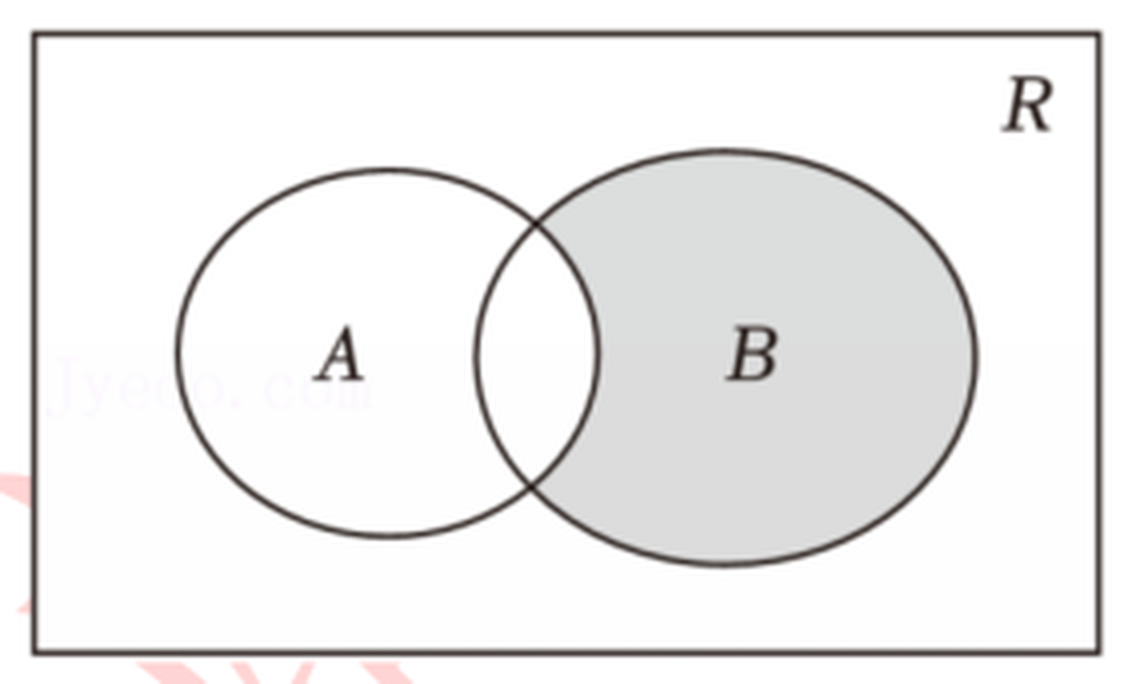
\includegraphics[width=0.30\textwidth]{figures/venn_Abar_cap_B.png}
\end{center}

\begin{enumerate}[label=(\arabic*)]
\item 若 $a=1$，求阴影部分表示的集合.
\item 若 $A\cap B=B$，求实数 $a$ 的取值范围.
\end{enumerate}

\ifanswer
\solbegin
\stepm{(1)}{因为 $\dfrac{2x-3}{x+5}\leqslant0$，
等价于 $\begin{cases}(2x-3)(x+5)\leqslant0\\ x+5\neq0\end{cases}$，}
\step{解得 $-5<x\leqslant\dfrac32$，即 $A=\left\{x\mid-5<x\leqslant\dfrac32\right\}$；}
\step{若 $a=1$，因为 $|x-1|<1$，等价于 $-1<x-1<1$，}
\step{解得 $0<x<2$，即 $B=\{x\mid0<x<2\}$.}
\step{由 Venn 图得阴影部分表示的集合为 $\overline{A}\cap B=\left(\dfrac32,2\right)$.}
\stepm{(2)}{由 (1) 得 $A=\left\{x\mid-5<x\leqslant\dfrac32\right\}$，}
\step{$B=\{x\mid|x-a|<1\}=\{x\mid-1+a<x<1+a\}\neq\varnothing$，}
\step{因为 $A\cap B=B$，所以 $B\sub A$，}
\step{所以 $\begin{cases}-5\leqslant-1+a\\ 1+a\leqslant\dfrac32\end{cases}$，
解得 $-4\leqslant a\leqslant\dfrac12$，}
\step{所以实数 $a$ 的取值范围为 $\left[-4,\dfrac12\right]$.}
\solend

\fi

\ansspace[6]

\item 设 $A=\{x\mid x^2-(m+3)x+2(m+1)=0,m\in\R\}$，
$B=\{x\mid 2x^2+(3n+1)x+2=0,n\in\R\}$.

\begin{enumerate}[label=(\arabic*)]
\item 是否存在 $m$、$n\in\R$，使得 $A=\{1,2\}$，$B=\varnothing$，说明理由；
\item 若 $A\cap B=A$，求 $m$、$n$ 的值.
\end{enumerate}

\ifanswer
\solbegin
\stepm{(1)}{由 $A=\{1,2\}$，得 $m=0$，}
\step{再由 $B=\varnothing$，得 $\Delta=(3n+1)^2-4\times2\times2=9n^2+6n-15<0$，}
\step{所以 $(3n+5)(n-1)<0$，解得 $-\dfrac53<n<1$，}
\step{故存在 $m=0$，$-\dfrac53<n<1$，使得 $A=\{1,2\}$，$B=\varnothing$.}
\stepm{(2)}{由 $x^2-(m+3)x+2(m+1)=0$，得 $x=2$ 或 $x=m+1$，}
\step{若 $A\cap B=A$，则 $A\sub B$，}
\step{将 $x=2$ 代入 $2x^2+(3n+1)x+2=0$，得 $n=-2$，}
\step{则 $B=\{x\mid 2x^2+(3n+1)x+2=0,n\in\R\}=\{x\mid 2x^2-5x+2=0\}
=\left\{2,\dfrac12\right\}$.}
\step{则 $m+1=\dfrac12$ 或 $m+1=2$，则 $m=-\dfrac12$ 或 $m=1$，
所以 $m=-\dfrac12$ 或 $m=1$，$n=-2$.}
\solend

\fi

\ansspace[6]

\item 已知陈述句 $\alpha$：关于 $x$ 的方程 $x^2-6x+m=0$ 有两个不同的正数根，陈述句
$\beta$：集合 $\{x\mid(m+1)x^2+4x+1=0,x\in\R\}$ 中至多有一个元素.

\begin{enumerate}[label=(\arabic*)]
\item 若 $\alpha$ 和 $\beta$ 都是真命题，求实数 $m$ 的取值范围；
\item 若 $\alpha$ 和 $\beta$ 至多有一个是假命题，求实数 $m$ 的取值范围.
\end{enumerate}

\ifanswer
\solbegin
\stepm{(1)}{因为关于 $x$ 的方程 $x^2-6x+m=0$ 有两个不同的正数根，}
\step{则 $\begin{cases}36-4m>0\\ m>0\end{cases}$，解得 $0<m<9$，}
\step{集合 $\{x\mid(m+1)x^2+4x+1=0,x\in\R\}$ 中至多有一个元素，}
\step{则 $m=-1$ 或 $\begin{cases}m+1\neq0\\ 16-4(m+1)\leqslant0\end{cases}$，
解得 $m\geqslant3$，}
\step{$\alpha$ 和 $\beta$ 都是真命题，所以实数 $m$ 的取值范围为 $\{m\mid3\leqslant m<9\}$}
\stepm{(2)}{由 (1) 得当 $\alpha$ 为假命题时，$m\leqslant0$ 或 $m\geqslant9$，}
\step{当 $\beta$ 为假命题时，$m<3$ 且 $m\neq-1$，}
\step{所以 $\alpha$ 和 $\beta$ 均为假命题时，$m$ 的范围是 $m\leqslant0$ 且 $m\neq-1$，}
\step{$\alpha$ 和 $\beta$ 至多有一个是假命题时，实数 $m$ 的取值范围为
$\{m\mid m>0$ 或 $m=-1\}$.}
\solend

\fi

\ansspace[6]

\item 已知符号 $[x]$ 表示不大于 $x$ 的最大整数 $(x\in\R)$，例如：$[1.3]=1$，
$[2]=2$，$[-1.2]=-2$.

\begin{enumerate}[label=(\arabic*)]
\item 已知方程 $[x]=3$，求该方程的解集；
\item 设方程 $\bigl[|x|+|x-1|\bigr]=3$ 的解集为 $A$，
集合 $B=\{x\mid 2x^2-11kx+15k^2\geqslant0\}$，若 $A\cup B=\R$，求实数 $k$ 的取值范围；
\item 在 (2) 的条件下，集合 $C=\{x\mid x^2-ax+1-2a\leqslant0,a\in\R\}$，是否存在实数
$a$，$A\cap C=A$，若存在，请求出实数 $a$ 的取值范围；若不存在，请说明理由.
\end{enumerate}

\ifanswer
\solbegin
\stepm{(1)}{方程 $[x]=3$，则 $x\in[3,4)$，所以该方程的解集为 $[3,4)$；}
\stepm{(2)}{因为 $\bigl[|x|+|x-1|\bigr]=3$，所以 $3\leqslant|x|+|x-1|<4$，}
\step{由绝对值不等式的几何意义得 $A=\left(-\dfrac32,-1\right]\cup\left[2,\dfrac52\right)$，}
\step{又 $B=\{x\mid 2x^2-11kx+15k^2\geqslant0\}=\{x\mid(2x-5k)(x-k)\geqslant0\}$，}
\step{当 $k=0$ 时，$B=\{x\mid 2x^2\geqslant0\}=\R$，则 $A\cup B=\R$，符合题意；}
\step{当 $k>0$ 时，$B=\left(-\infty,\dfrac{5k}{2}\right]\cup[3k,+\infty)$，
若 $A\cup B=\R$，}
\step{则 $\begin{cases}\dfrac{5k}{2}\geqslant2\\[2pt] 3k\leqslant\dfrac52\end{cases}$，
解得 $k\in\left[\dfrac45,\dfrac56\right]$；}
\step{当 $k<0$ 时，$B=(-\infty,3k]\cup\left[\dfrac{5k}{2},+\infty\right)$，
若 $A\cup B=\R$，}
\step{则 $\begin{cases}\dfrac{5k}{2}\leqslant-1\\[2pt] 3k\geqslant-\dfrac32\end{cases}$，
解得 $k\in\left[-\dfrac12,-\dfrac25\right]$.}
\step{综上所述，实数 $k$ 的取值范围为
$\left[-\dfrac12,-\dfrac25\right]\cup\{0\}\cup\left[\dfrac45,\dfrac56\right]$；}
\stepm{(3)}{因为 $A\cap C=A$，则 $A\sub C$ 且
$A=\left(-\dfrac32,-1\right]\cup\left[2,\dfrac52\right)$，}
\step{设集合 $C$ 的解集为 $(x_1,x_2)(x_1<x_2)$，}
\step{则 $\begin{cases}x_1\leqslant-\dfrac32\\[2pt] x_2\geqslant\dfrac52\end{cases}$，}
\step{所以
$\begin{cases}\Delta=a^2-4(1-2a)>0\\[2pt]
f\!\left(-\dfrac32\right)=\dfrac94+\dfrac32a+1-2a\leqslant0\\[4pt]
f\!\left(\dfrac52\right)=\dfrac{25}{4}-\dfrac52a+1-2a\leqslant0\end{cases}$，
解得 $a\geqslant\dfrac{13}{2}$，}
\step{故实数 $a$ 的取值范围为 $\left[\dfrac{13}{2},+\infty\right)$.}
\solend

\fi

\ansspace[6]

\item 非空有限集合 $S$ 是由若干个正实数组成，集合 $S$ 的元素个数不少于 $2$ 个. 对于任意
$a,b\in S,a\neq b$，若数 $a^b$ 或 $b^a$ 中至少有一个属于 $S$，则称集合 $S$ 是“好集”；
否则，称集合 $S$ 是“坏集”.

\begin{enumerate}[label=(\arabic*)]
\item 判断 $A=\{1,3,9\}$ 和 $B=\left\{1,\dfrac12,\dfrac14,\dfrac1{16}\right\}$ 是“好集”
还是“坏集”，并简单说明理由；
\item 题设的有限集 $S$ 中，既有大于 $1$ 的元素，又有小于 $1$ 的元素，证明：集合 $S$ 是
“坏集”；
\item 若题设中的 $a^b$ 或 $b^a$ 都属于 $S$，则称集合 $S$ 为“超级好集”，写出一个
“超级好集”（无须证明）.
\end{enumerate}

\ifanswer
\solbegin
\stepm{(1)}{$A=\{1,3,9\}$，$3^9\notin A$，$9^3\notin A$，所以 $A$ 是“坏集”，}
\step{从 $B$ 集合中任意取两个数字都满足需求，所以 $B$ 是“好集”.}
\stepm{(2)}{假设 $a$ 是 $S$ 中小于 $1$ 的元素中的最小元素，}
\step{$b$ 是 $S$ 中大于 $1$ 的元素中的最小元素，则 $a^b<a^1=a$，}
\step{所以 $a$ 就不是 $S$ 中小于 $1$ 的元素中的最小元素，即 $a^b\notin S$，}
\step{同理 $1=b^0<b^a<b^1=b$，所以 $b$ 就不是 $S$ 中大于 $1$ 的元素中的最小元素，}
\step{即 $b^a\notin S$，所以集合 $S$ 是“坏集”；}
\stepm{(3)}{首先 $S=\{1,a\}$（$a\neq1$ 且 $a>0$）是“超级好集”，}
\step{假设 $0<a<1$，由 (2) 得，$S$ 中不可能有大于 $1$ 的元素，}
\step{假设 $S$ 中有除 $a$ 之外的元素 $b\in S$（$a\neq b,b<1$），}
\step{假设 $a$ 是 $S$ 中小于 $1$ 的元素中的最大元素，$a^b>a^1=a$，}
\step{所以 $a$ 不是最大元素，所以 $a^b\notin S$，所以 $b\notin S$；}
\step{假设 $a>1$，由 (2) 得 $S$ 中不可能有小于 $1$ 的元素，}
\step{假设 $S$ 中有除 $a$ 之外的元素 $b$（$b>1$ 且 $b\neq a$），}
\step{假设 $a$ 是 $S$ 中大于 $1$ 的元素中的最小元素，则 $a^b>a^1=a$，}
\step{所以 $a$ 不是最小元素，即不存在 $b>1$，使得 $b\in S$，即 $b\notin S$，}
\step{综上，$S=\{1,a\}$（$a\neq1$ 且 $a>0$）.}
\solend

\fi

\ansspace*[10]

\end{enumerate}

\end{document}
"
% 紧凑版：xelatex "\def\iscompact{1}% 高一25_华师大二附中_周末作业3.tex
%   —— 高一上数学「2026-2027 年华师大二附中高一上周末作业 3」（试卷版/答案版）
% 试卷版：xelatex 高一25_华师大二附中_周末作业3.tex
% 答案版：xelatex "\def\isanswer{1}% 高一25_华师大二附中_周末作业3.tex
%   —— 高一上数学「2026-2027 年华师大二附中高一上周末作业 3」（试卷版/答案版）
% 试卷版：xelatex 高一25_华师大二附中_周末作业3.tex
% 答案版：xelatex "\def\isanswer{1}% 高一25_华师大二附中_周末作业3.tex
%   —— 高一上数学「2026-2027 年华师大二附中高一上周末作业 3」（试卷版/答案版）
% 试卷版：xelatex 高一25_华师大二附中_周末作业3.tex
% 答案版：xelatex "\def\isanswer{1}\input{高一25_华师大二附中_周末作业3.tex}"
% 紧凑版：xelatex "\def\iscompact{1}\input{高一25_华师大二附中_周末作业3.tex}"
%
% 原始材料是微信公众号图文（公众号「魔都数学加油站」连载「27学年高一 25」，2026-09-21 发布，
% 原文标题「27学年高一25——2026-2027年上海市华师大二附中高一上周末作业3」），
% 正文为 10 张 PNG 页（1080×1527，各页同尺寸）。原文本身就是一份**讲评版**——
% 题目下方直接印出【解析】（本卷无单独的【答案】行，填空题答案都写在解析里）。
% 试题文字与解析均照原卷录入，未改内容。卷面的粉色斜水印「魔都数学加油站」属水印，未录入。
%
% 卷首标题：原卷印作「2026-2027 年华师大二附中高一上周末作业 3」（公众号标题里的「上海市」
% 三字卷面标题行没有，本稿照卷面），年份区间按全稿惯例排 en dash，前缀照原卷保留「年」。
%
% 与原卷的排版差异（均已在 README「说明」中交代）：
%   ① 原文自**第 3 题**起（第 1、2 题未在该文中发布），故本稿题号亦自 3 起；
%   ② 原卷本就印有「一、填空题」「二、选择题」「三、解答题」三节标题，本稿照原卷分节，
%      只把标题改排成全稿统一的「大节标题」样式；
%   ③ 原卷第 13 题的答案「D」直接印在题干末尾的括号内，第 14—16 题的括号空着、答案写在
%      解析末句「故选 C／B」里；填空题的答案也都嵌在解析里，本稿统一改为试卷版隐去、
%      答案版以 \ans{} 给出（选择题另附【解析】），使两版彻底分离；
%   ④ 补集符号原卷一律作**上横线**（$\overline{A}$、$\overline{A\cup B}$），与同校的
%      高一14 同例，本稿照录（不改为 $\complement_U A$ 写法）；
%   ⑤ 原卷的实数集 R 斜体与粗体混用（第 17 题题干「全集为 R」作粗体，第 5、14 题与
%      第 16 题解析的 $R$ 为斜体），本稿按全稿惯例统一写作 $\R$；
%   ⑥ 原卷填空的横线约两个字宽，本稿按全稿惯例统一排 \blankline[4.4em]；
%   ⑦ 原卷未印副标题，本稿按全稿惯例补出副标题「集合与常用逻辑用语」；
%   ⑧ 第 17 题的 Venn 图原卷印在题干右侧（第 6 页），本稿移至题干之后；
%      图取原卷截图、4× LANCZOS 放大（figures/venn_Abar_cap_B.png，
%      阴影为 $B$ 中不含 $A\cap B$ 的部分，即 $\overline{A}\cap B$）。
%
% 原卷存疑两处（均照抄原卷、未改，见源码中该处上方注释）：
%   ① 第 8 题【解析】第二段「当 $\Delta=a^2-16>0$ 时，方程 $x^2+ax+4=0$ 有两个相同的根
%      $x_1$、$x_2$」——$\Delta>0$ 应为「两个**不**相同的根」（其自己的后文就把 $x_1$、$x_2$
%      当作可以不同的两个根在讨论），显系笔误；
%   ② 第 11 题【解析】先写「偶数必是 $2^{11}\cdot3^m\cdot337^n$，$m$、$n\in\N^*$」，
%      下一行又写「$0\leqslant m\leqslant10$，$0\leqslant n\leqslant10$，共有 121 种情况」
%      ——按 $\N^*$ 应从 1 起（至多 $10\times10=100$ 种），与 121（$=11\times11$，含 0）
%      对不上，两处至少有一处笔误。

\documentclass[a4paper,11pt]{article}
\usepackage{common}

\begin{document}

\examtitlest[3]{2026--2027 年华师大二附中高一上周末作业 3}{集合与常用逻辑用语}

\bigsec{一、填空题}

\begin{enumerate}
\setcounter{enumi}{2}

\item 设全集 $U=\{2,4,m^2+m-5\}$，集合 $A=\{2,1-m\}$，若 $\overline{A}=\{1\}$，则实数
$m=$ \blankline[4.4em].

\ifanswer
\solbegin
\step{因为 $\overline{A}=\{1\}$，所以 $1\in U$，$1\notin A$，}
\step{所以 $\begin{cases}m^2+m-5=1\\ 1-m\neq1\\ 1-m=4\end{cases}$，解得 $m=-3$.}
\solend

\fi

\item 已知条件 $\alpha$：$m<x\leqslant2m+5$，条件 $\beta$：$0\leqslant x\leqslant1$，
若 $\alpha$ 是 $\beta$ 的必要条件，则实数 $m$ 的取值范围为 \blankline[4.4em].

\ifanswer
\solbegin
\step{若 $\alpha$ 是 $\beta$ 的必要条件，则 $[0,1]\sub(m,2m+5]$，}
\step{所以 $\begin{cases}m<2m+5\\ m<0\\ 2m+5\geqslant1\end{cases}$，}
\step{解得 $-2\leqslant m<0$，故实数 $m$ 的取值范围为 $[-2,0)$.}
\solend

\fi

\item 已知 $\R$ 是全集，集合 $A=\{y\mid y=-x^2+1,x\in\R\}$，集合
$B=\{x\mid x=3+|a|,a\in\R\}$，则 $\overline{A\cup B}=$ \blankline[4.4em].

\ifanswer
\solbegin
\step{$A=\{y\mid y=-x^2+1,x\in\R\}=(-\infty,1]$，}
\step{$B=\{x\mid x=3+|a|,a\in\R\}=[3,+\infty)$，}
\step{所以 $\overline{A\cup B}=(1,3)$.}
\solend

\fi

\item 已知 $a$ 为常数，集合 $A=\{x\mid x^2+x-6=0\}$，集合 $B=\{x\mid ax-2=0\}$，且
$B\sub A$，则 $a$ 的所有取值构成的集合为 \blankline[4.4em].

\ifanswer
\solbegin
\step{集合 $A=\{-3,2\}$，因为 $B\sub A$，所以 $B=\varnothing$，$\{-3\}$，$\{2\}$，$\{-3,2\}$，}
\step{当 $B=\varnothing$ 时，$a=0$，当 $B=\{-3\}$ 时，$a=-\dfrac23$，当 $B=\{2\}$ 时，$a=1$，}
\step{当 $B=\{-3,2\}$ 时，不成立，故 $a$ 的取值集合为 $\left\{0,-\dfrac23,1\right\}$.}
\solend

\fi

\item 已知一元二次方程 $x^2+px+p=0$ 有两个不相等的实根分别为 $x_1$、$x_2$.
$A=x_1^2+x_2^2$，$B=x_1x_2(x_1+x_2)$，$A$ 与 $B$ 的大小为 \blankline[4.4em].

\ifanswer
\solbegin
\step{一元二次方程 $x^2+px+p=0$ 有两个不相等的实根分别为 $x_1$、$x_2$，}
\step{则 $\Delta=p^2-4p>0$，解得 $p<0$ 或 $p>4$，}
\step{由韦达定理得 $x_1+x_2=-p$，$x_1x_2=p$，}
\step{所以 $A=x_1^2+x_2^2=(x_1+x_2)^2-2x_1x_2=p^2-2p$，$B=x_1x_2(x_1+x_2)=-p^2$，}
\step{所以 $A-B=(p^2-2p)-(-p^2)=2p(p-1)$，}
\step{当 $p<0$ 时，则 $A-B>0$，故 $A>B$，}
\step{当 $p>4$ 时，则 $A-B>0$，故 $A>B$，}
\step{综上，$A=p^2-2p$，$B=-p^2$，且 $A>B$.}
\solend

\fi

\item 集合 $A=\{x\mid(x-1)(x^2+ax+4)=0,x\in\R\}$ 中所有元素之和为 $3$，则实数
$a=$ \blankline[4.4em].

\ifanswer
\solbegin
\step{当 $\Delta=a^2-16=0$ 时，方程 $x^2+ax+4=0$ 有两个相同的根 $-\dfrac a2$，}
\step{则 $A=\left\{1,-\dfrac a2\right\}$，故 $1-\dfrac a2=3$，解得 $a=-4$；}
% 注：下一行的「两个相同的根」系原卷笔误（△>0 应为「两个不相同的根」，其自己的后文
%     就把 x₁、x₂ 当作可以不同的两个根在讨论），照抄原卷、未改，见文件头「原卷存疑」①。
\step{当 $\Delta=a^2-16>0$ 时，方程 $x^2+ax+4=0$ 有两个相同的根 $x_1$、$x_2$，}
\step{若 $1$ 是方程 $x^2+ax+4=0$ 的根，则方程 $x^2+ax+4=0$ 的另一个根为 $4$，}
\step{则 $A=\{1,4\}$，不成立；}
\step{若 $1$ 不是方程 $x^2+ax+4=0$ 的根，则 $A=\{1,x_1,x_2\}$，则 $1+x_1+x_2=3$，}
\step{故 $x_1+x_2=2=-a$，故 $a=-2$（舍去）；}
\step{综上所述，$a=-4$.}
\solend

\fi

\item 已知集合 $A=\{x\mid x^2+2x-8\geqslant0\}$，$B=\{x\mid x^2-2ax+4\leqslant0\}$，
若 $a>0$，且 $A\cap B\cap\N$ 中恰有 $2$ 个元素，则 $a$ 的取值范围为 \blankline[4.4em].

\ifanswer
\solbegin
\step{由 $A$ 中不等式变形得 $(x-2)(x+4)\geqslant0$，解得 $x\leqslant-4$ 或 $x\geqslant2$，}
\step{即 $A=(-\infty,-4]\cup[2,+\infty)$，}
\step{设 $f(x)=x^2-2ax+4$，则 $f(x)$ 的轴对称 $x=a>0$，}
\step{且对应方程的根 $x_1$、$x_2$ 满足 $\begin{cases}x_1x_2=4\\ x_1+x_2>0\end{cases}$，}
\step{所以 $0<x_1\leqslant2\leqslant x_2$（取 $x_1\leqslant x_2$），}
\step{所以 $A\cap B\cap\N$ 中恰有的整数为 $2$，$3$，}
\step{所以 $\begin{cases}f(3)=9-6a+4\leqslant0\\ f(4)=16-8a+4>0\end{cases}$，}
\step{解得 $\dfrac{13}{6}\leqslant a<\dfrac52$，所以 $a$ 的取值范围为 $\left[\dfrac{13}{6},\dfrac52\right)$.}
\solend

\fi

\item 在三个关于 $x$ 的方程 $x^2-ax+4=0$，$x^2+(a-1)x+16=0$ 和
$x^2+2ax+3a+10=0$ 中至少有一个方程有实根，则实数 $a$ 的取值范围是 \blankline[4.4em].

\ifanswer
\solbegin
\step{当三个方程均无实根时，有}
\step{$\begin{cases}\Delta_1=a^2-16<0\\ \Delta_2=(a-1)^2-64<0\\ \Delta_3=4a^2-4(3a+10)<0\end{cases}$，}
\step{所以 $\begin{cases}-4<a<4\\ -7<a<9\\ -2<a<5\end{cases}$，}
\step{所以 $-2<a<4$，故三个方程均无实根时，$a$ 的取值范围为 $(-2,4)$，}
\step{所以三个方程中至少有一个方程有实根时，}
\step{实数 $a$ 的取值范围为 $(-\infty,-2]\cup[4,+\infty)$.}
\solend

\fi

% 注：下一行解析里的「m、n∈N*」与再下一行的「0≤m≤10，0≤n≤10，共有 121 种情况」
%     对不上（按 N* 应从 1 起，至多 10×10=100 种；121=11×11 含 0），系原卷自身矛盾，
%     照抄原卷、未改，见文件头「原卷存疑」②。
\item 若集合 $M=\{(x,y)\mid(x+1)+(x+2)+\cdots+(x+y)=2022^{10},x\in\Z,y\in\N^{*}\}$，
则集合 $M$ 中元素有 \blankline[4.4em] 个.

\ifanswer
\solbegin
\step{由题意得 $(x+1)+(x+2)+\cdots+(x+y)=\dfrac{y(2x+1+y)}{2}$，}
\step{所以 $y(2x+1+y)=2^{11}\cdot3^{10}\cdot337^{10}$，}
\step{因为 $y$ 与 $2x+1+y$ 必为一奇一偶，偶数必是 $2^{11}\cdot3^m\cdot337^n$，
$m$、$n\in\N^{*}$，}
\step{$0\leqslant m\leqslant10$，$0\leqslant n\leqslant10$，共有 $121$ 种情况，}
\step{因为 $y$ 与 $2x+1+y$ 奇偶未定，所以集合 $M$ 中元素只有 $242$ 个.}
\solend

\fi

\item 设集合 $M=\left\{x\mid m\leqslant x\leqslant m+\dfrac34\right\}$，
$N=\left\{x\mid n-\dfrac13\leqslant x\leqslant n\right\}$，且 $M$、$N$ 都是集合
$\{x\mid0\leqslant x\leqslant1\}$ 的子集，如果把 $b-a$ 叫做集合
$\{x\mid a\leqslant x\leqslant b\}$ 的长度，那么集合 $M\cap N$ 的长度的最小值是
\blankline[4.4em].

\ifanswer
\solbegin
\step{$M$ 的长度为 $\dfrac34$，$N$ 的长度为 $\dfrac13$，}
\step{当集合 $M\cap N$ 的长度的最小值时，$M$ 与 $N$ 应分别在区间 $[0,1]$ 的左右两端，}
\step{故 $M\cap N$ 的长度的最小值是 $\dfrac34+\dfrac13-1=\dfrac1{12}$.}
\solend

\fi

\end{enumerate}

\bigsec{二、选择题}

\begin{enumerate}
\setcounter{enumi}{12}

\item 直角坐标平面中除去两点 $A(1,1)$、$B(2,-2)$ 可用集合表示为\mbox{（\quad）}

\keepwithprev
A. $\{(x,y)\mid x\neq1,y\neq1,x\neq2,y\neq-2$\}\qquad
B. $\{(x,y)\mid\begin{cases}x\neq1\\ y\neq1\end{cases}$ 或 $\begin{cases}x\neq2\\ y\neq-2\end{cases}\}$

C. $\{(x,y)\mid[(x-1)^2+(y-1)^2][(x-2)^2+(y+2)^2]\neq0$\}

D. $\{(x,y)\mid[(x-1)^2+(y-1)^2]+[(x-2)^2+(y+2)^2]\neq0$\}

\ans{$D$}

\item 已知函数 $f(x)=x^2+nx$，记集合 $A=\{x\mid f(x)=0,x\in\R\}$，
$B=\{x\mid f(f(x))=0,x\in\R\}$，若 $A=B\neq\varnothing$，则 $n$ 的取值范围是\mbox{（\quad）}

\keepwithprev
A. $[0,4]$\qquad B. $(0,4)$\qquad C. $[0,4)$\qquad D. $(0,4]$

\ans{$C$}

\ifanswer
\solbegin
\step{$f(x)=x^2+nx$，$f[f(x)]=(x^2+nx)^2+n(x^2+nx)=(x^2+nx)(x^2+nx+n)$，}
\step{当 $n=0$ 时，$f(x)=x^2$，$f[f(x)]=x^4$，满足 $A=B$，此时 $n=0$；}
\step{当 $n\neq0$ 时，$0$、$-n$ 不是 $x^2+nx+n=0$ 的根，故 $\Delta=n^2-4n<0$，
解得 $0<n<4$，}
\step{综上所述，$n$ 的取值范围是 $[0,4)$. 故选 $C$.}
\solend

\fi

\item 设全集 $U=\{1,2,3,4,5,6,7,8,9,10\}$，给出条件：① $A\sub U$；②若 $x\in A$，
则 $2x\notin A$；③若 $x\in\overline{A}$，则 $2x\notin\overline{A}$.
那么同时满足三个条件的集合 $A$ 的个数为\mbox{（\quad）}

\keepwithprev
A. $0$ 个\qquad B. $16$ 个\qquad C. $32$ 个\qquad D. $64$ 个

\ans{$C$}

\ifanswer
\solbegin
\step{由① $A\sub U$；②若 $x\in A$，则 $2x\notin A$；③若 $x\in\overline{A}$，
则 $2x\notin\overline{A}$.}
\step{若 $1\in A$，则 $2\notin A$，即 $2\in\overline{A}$，则 $4\notin\overline{A}$，
即 $4\in A$，则 $8\notin A$，即 $8\in\overline{A}$；}
\step{若 $3\in A$，则 $6\notin A$，即 $6\in\overline{A}$；若 $5\in A$，则 $10\notin A$，
即 $10\in\overline{A}$，}
\step{故 $1$、$4$ 和 $2$、$8$ 分开，$3$ 和 $6$ 分开，$5$ 和 $10$ 分开，$7$ 和 $9$ 随意，}
\step{故同时满足三个条件的集合 $A$ 的个数为 $2\times2\times2\times2\times2=32$，
故选 $C$.}
\solend

\fi

\item 设集合 $P_1=\{x\mid x^2+ax+1>0\}$，$P_2=\{x\mid x^2+ax+2>0\}$，
$Q_1=\{x\mid x^2+x+b>0\}$，$Q_2=\{x\mid x^2+2x+b>0\}$，其中 $a$、$b\in\R$，
下列说法中正确的是\mbox{（\quad）}

\keepwithprev
A. 对任意 $a$，$P_1$ 是 $P_2$ 的子集，对任意的 $b$，$Q_1$ 不是 $Q_2$ 的子集

B. 对任意 $a$，$P_1$ 是 $P_2$ 的子集，存在 $b$，使得 $Q_1$ 是 $Q_2$ 的子集

C. 存在 $a$，使得 $P_1$ 不是 $P_2$ 的子集，对任意的 $b$，$Q_1$ 不是 $Q_2$ 的子集

D. 存在 $a$，使得 $P_1$ 不是 $P_2$ 的子集，存在 $b$，使得 $Q_1$ 是 $Q_2$ 的子集

\ans{$B$}

\ifanswer
\solbegin
\step{对于集合 $P_1=\{x\mid x^2+ax+1>0\}$，$P_2=\{x\mid x^2+ax+2>0\}$，}
\step{得当 $m\in P_1$ 时，即 $m^2+am+1>0$，得 $m^2+am+2>0$，}
\step{即有 $m\in P_2$，得对任意 $a$，$P_1$ 是 $P_2$ 的子集，}
\step{对于集合 $Q_1=\{x\mid x^2+x+b>0\}$，$Q_2=\{x\mid x^2+2x+b>0\}$，}
\step{当 $b=6$ 时，$Q_1=\{x\mid x^2+x+6>0\}=\R$，$Q_2=\{x\mid x^2+2x+6>0\}=\R$，}
\step{得 $Q_1$ 是 $Q_2$ 的子集，}
\step{当 $b=1$ 时，$Q_1=\{x\mid x^2+x+1>0\}=\R$，}
\step{$Q_2=\{x\mid x^2+2x+1>0\}=\{x\mid x\neq-1\}$，得 $Q_1$ 不是 $Q_2$ 的子集，}
\step{所以存在 $b$，使得 $Q_1$ 是 $Q_2$ 的子集，故选 $B$.}
\solend

\fi

\end{enumerate}

\bigsec{三、解答题}

\begin{enumerate}
\setcounter{enumi}{16}

\item 已知集合 $A=\left\{x\mid\dfrac{2x-3}{x+5}\leqslant0\right\}$，
$B=\{x\mid|x-a|<1\}$，全集为 $\R$.

\begin{center}
% 图取原卷截图、4× LANCZOS 放大（原卷把图印在题干右侧，本稿移至此处，见文件头⑧）。
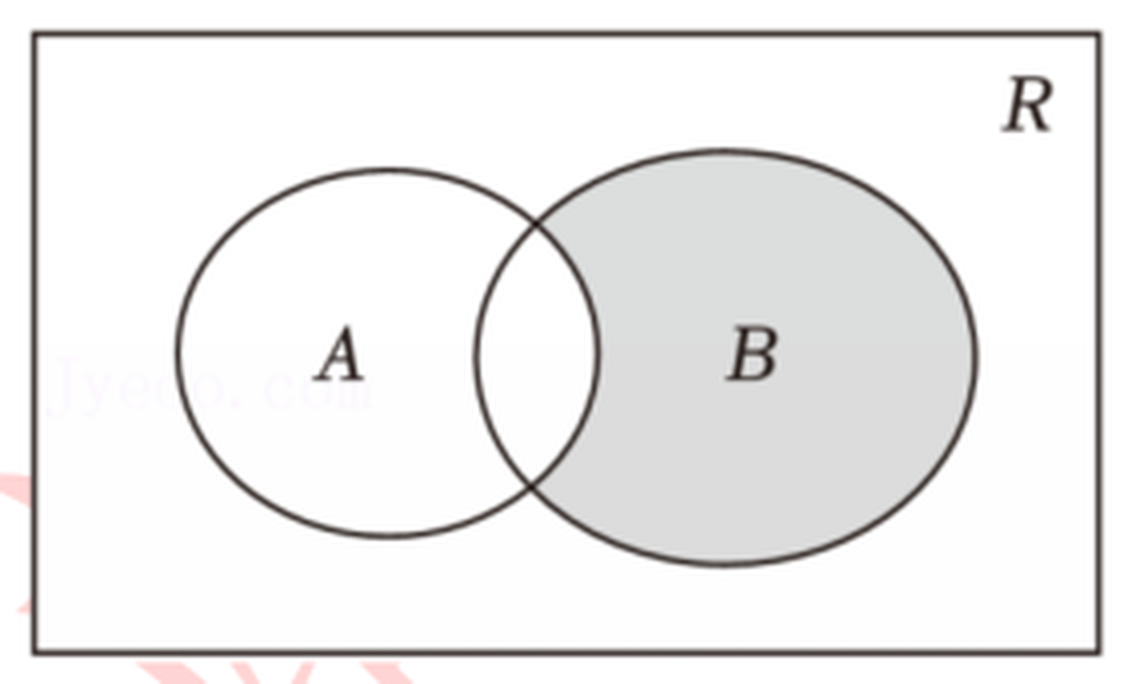
\includegraphics[width=0.30\textwidth]{figures/venn_Abar_cap_B.png}
\end{center}

\begin{enumerate}[label=(\arabic*)]
\item 若 $a=1$，求阴影部分表示的集合.
\item 若 $A\cap B=B$，求实数 $a$ 的取值范围.
\end{enumerate}

\ifanswer
\solbegin
\stepm{(1)}{因为 $\dfrac{2x-3}{x+5}\leqslant0$，
等价于 $\begin{cases}(2x-3)(x+5)\leqslant0\\ x+5\neq0\end{cases}$，}
\step{解得 $-5<x\leqslant\dfrac32$，即 $A=\left\{x\mid-5<x\leqslant\dfrac32\right\}$；}
\step{若 $a=1$，因为 $|x-1|<1$，等价于 $-1<x-1<1$，}
\step{解得 $0<x<2$，即 $B=\{x\mid0<x<2\}$.}
\step{由 Venn 图得阴影部分表示的集合为 $\overline{A}\cap B=\left(\dfrac32,2\right)$.}
\stepm{(2)}{由 (1) 得 $A=\left\{x\mid-5<x\leqslant\dfrac32\right\}$，}
\step{$B=\{x\mid|x-a|<1\}=\{x\mid-1+a<x<1+a\}\neq\varnothing$，}
\step{因为 $A\cap B=B$，所以 $B\sub A$，}
\step{所以 $\begin{cases}-5\leqslant-1+a\\ 1+a\leqslant\dfrac32\end{cases}$，
解得 $-4\leqslant a\leqslant\dfrac12$，}
\step{所以实数 $a$ 的取值范围为 $\left[-4,\dfrac12\right]$.}
\solend

\fi

\ansspace[6]

\item 设 $A=\{x\mid x^2-(m+3)x+2(m+1)=0,m\in\R\}$，
$B=\{x\mid 2x^2+(3n+1)x+2=0,n\in\R\}$.

\begin{enumerate}[label=(\arabic*)]
\item 是否存在 $m$、$n\in\R$，使得 $A=\{1,2\}$，$B=\varnothing$，说明理由；
\item 若 $A\cap B=A$，求 $m$、$n$ 的值.
\end{enumerate}

\ifanswer
\solbegin
\stepm{(1)}{由 $A=\{1,2\}$，得 $m=0$，}
\step{再由 $B=\varnothing$，得 $\Delta=(3n+1)^2-4\times2\times2=9n^2+6n-15<0$，}
\step{所以 $(3n+5)(n-1)<0$，解得 $-\dfrac53<n<1$，}
\step{故存在 $m=0$，$-\dfrac53<n<1$，使得 $A=\{1,2\}$，$B=\varnothing$.}
\stepm{(2)}{由 $x^2-(m+3)x+2(m+1)=0$，得 $x=2$ 或 $x=m+1$，}
\step{若 $A\cap B=A$，则 $A\sub B$，}
\step{将 $x=2$ 代入 $2x^2+(3n+1)x+2=0$，得 $n=-2$，}
\step{则 $B=\{x\mid 2x^2+(3n+1)x+2=0,n\in\R\}=\{x\mid 2x^2-5x+2=0\}
=\left\{2,\dfrac12\right\}$.}
\step{则 $m+1=\dfrac12$ 或 $m+1=2$，则 $m=-\dfrac12$ 或 $m=1$，
所以 $m=-\dfrac12$ 或 $m=1$，$n=-2$.}
\solend

\fi

\ansspace[6]

\item 已知陈述句 $\alpha$：关于 $x$ 的方程 $x^2-6x+m=0$ 有两个不同的正数根，陈述句
$\beta$：集合 $\{x\mid(m+1)x^2+4x+1=0,x\in\R\}$ 中至多有一个元素.

\begin{enumerate}[label=(\arabic*)]
\item 若 $\alpha$ 和 $\beta$ 都是真命题，求实数 $m$ 的取值范围；
\item 若 $\alpha$ 和 $\beta$ 至多有一个是假命题，求实数 $m$ 的取值范围.
\end{enumerate}

\ifanswer
\solbegin
\stepm{(1)}{因为关于 $x$ 的方程 $x^2-6x+m=0$ 有两个不同的正数根，}
\step{则 $\begin{cases}36-4m>0\\ m>0\end{cases}$，解得 $0<m<9$，}
\step{集合 $\{x\mid(m+1)x^2+4x+1=0,x\in\R\}$ 中至多有一个元素，}
\step{则 $m=-1$ 或 $\begin{cases}m+1\neq0\\ 16-4(m+1)\leqslant0\end{cases}$，
解得 $m\geqslant3$，}
\step{$\alpha$ 和 $\beta$ 都是真命题，所以实数 $m$ 的取值范围为 $\{m\mid3\leqslant m<9\}$}
\stepm{(2)}{由 (1) 得当 $\alpha$ 为假命题时，$m\leqslant0$ 或 $m\geqslant9$，}
\step{当 $\beta$ 为假命题时，$m<3$ 且 $m\neq-1$，}
\step{所以 $\alpha$ 和 $\beta$ 均为假命题时，$m$ 的范围是 $m\leqslant0$ 且 $m\neq-1$，}
\step{$\alpha$ 和 $\beta$ 至多有一个是假命题时，实数 $m$ 的取值范围为
$\{m\mid m>0$ 或 $m=-1\}$.}
\solend

\fi

\ansspace[6]

\item 已知符号 $[x]$ 表示不大于 $x$ 的最大整数 $(x\in\R)$，例如：$[1.3]=1$，
$[2]=2$，$[-1.2]=-2$.

\begin{enumerate}[label=(\arabic*)]
\item 已知方程 $[x]=3$，求该方程的解集；
\item 设方程 $\bigl[|x|+|x-1|\bigr]=3$ 的解集为 $A$，
集合 $B=\{x\mid 2x^2-11kx+15k^2\geqslant0\}$，若 $A\cup B=\R$，求实数 $k$ 的取值范围；
\item 在 (2) 的条件下，集合 $C=\{x\mid x^2-ax+1-2a\leqslant0,a\in\R\}$，是否存在实数
$a$，$A\cap C=A$，若存在，请求出实数 $a$ 的取值范围；若不存在，请说明理由.
\end{enumerate}

\ifanswer
\solbegin
\stepm{(1)}{方程 $[x]=3$，则 $x\in[3,4)$，所以该方程的解集为 $[3,4)$；}
\stepm{(2)}{因为 $\bigl[|x|+|x-1|\bigr]=3$，所以 $3\leqslant|x|+|x-1|<4$，}
\step{由绝对值不等式的几何意义得 $A=\left(-\dfrac32,-1\right]\cup\left[2,\dfrac52\right)$，}
\step{又 $B=\{x\mid 2x^2-11kx+15k^2\geqslant0\}=\{x\mid(2x-5k)(x-k)\geqslant0\}$，}
\step{当 $k=0$ 时，$B=\{x\mid 2x^2\geqslant0\}=\R$，则 $A\cup B=\R$，符合题意；}
\step{当 $k>0$ 时，$B=\left(-\infty,\dfrac{5k}{2}\right]\cup[3k,+\infty)$，
若 $A\cup B=\R$，}
\step{则 $\begin{cases}\dfrac{5k}{2}\geqslant2\\[2pt] 3k\leqslant\dfrac52\end{cases}$，
解得 $k\in\left[\dfrac45,\dfrac56\right]$；}
\step{当 $k<0$ 时，$B=(-\infty,3k]\cup\left[\dfrac{5k}{2},+\infty\right)$，
若 $A\cup B=\R$，}
\step{则 $\begin{cases}\dfrac{5k}{2}\leqslant-1\\[2pt] 3k\geqslant-\dfrac32\end{cases}$，
解得 $k\in\left[-\dfrac12,-\dfrac25\right]$.}
\step{综上所述，实数 $k$ 的取值范围为
$\left[-\dfrac12,-\dfrac25\right]\cup\{0\}\cup\left[\dfrac45,\dfrac56\right]$；}
\stepm{(3)}{因为 $A\cap C=A$，则 $A\sub C$ 且
$A=\left(-\dfrac32,-1\right]\cup\left[2,\dfrac52\right)$，}
\step{设集合 $C$ 的解集为 $(x_1,x_2)(x_1<x_2)$，}
\step{则 $\begin{cases}x_1\leqslant-\dfrac32\\[2pt] x_2\geqslant\dfrac52\end{cases}$，}
\step{所以
$\begin{cases}\Delta=a^2-4(1-2a)>0\\[2pt]
f\!\left(-\dfrac32\right)=\dfrac94+\dfrac32a+1-2a\leqslant0\\[4pt]
f\!\left(\dfrac52\right)=\dfrac{25}{4}-\dfrac52a+1-2a\leqslant0\end{cases}$，
解得 $a\geqslant\dfrac{13}{2}$，}
\step{故实数 $a$ 的取值范围为 $\left[\dfrac{13}{2},+\infty\right)$.}
\solend

\fi

\ansspace[6]

\item 非空有限集合 $S$ 是由若干个正实数组成，集合 $S$ 的元素个数不少于 $2$ 个. 对于任意
$a,b\in S,a\neq b$，若数 $a^b$ 或 $b^a$ 中至少有一个属于 $S$，则称集合 $S$ 是“好集”；
否则，称集合 $S$ 是“坏集”.

\begin{enumerate}[label=(\arabic*)]
\item 判断 $A=\{1,3,9\}$ 和 $B=\left\{1,\dfrac12,\dfrac14,\dfrac1{16}\right\}$ 是“好集”
还是“坏集”，并简单说明理由；
\item 题设的有限集 $S$ 中，既有大于 $1$ 的元素，又有小于 $1$ 的元素，证明：集合 $S$ 是
“坏集”；
\item 若题设中的 $a^b$ 或 $b^a$ 都属于 $S$，则称集合 $S$ 为“超级好集”，写出一个
“超级好集”（无须证明）.
\end{enumerate}

\ifanswer
\solbegin
\stepm{(1)}{$A=\{1,3,9\}$，$3^9\notin A$，$9^3\notin A$，所以 $A$ 是“坏集”，}
\step{从 $B$ 集合中任意取两个数字都满足需求，所以 $B$ 是“好集”.}
\stepm{(2)}{假设 $a$ 是 $S$ 中小于 $1$ 的元素中的最小元素，}
\step{$b$ 是 $S$ 中大于 $1$ 的元素中的最小元素，则 $a^b<a^1=a$，}
\step{所以 $a$ 就不是 $S$ 中小于 $1$ 的元素中的最小元素，即 $a^b\notin S$，}
\step{同理 $1=b^0<b^a<b^1=b$，所以 $b$ 就不是 $S$ 中大于 $1$ 的元素中的最小元素，}
\step{即 $b^a\notin S$，所以集合 $S$ 是“坏集”；}
\stepm{(3)}{首先 $S=\{1,a\}$（$a\neq1$ 且 $a>0$）是“超级好集”，}
\step{假设 $0<a<1$，由 (2) 得，$S$ 中不可能有大于 $1$ 的元素，}
\step{假设 $S$ 中有除 $a$ 之外的元素 $b\in S$（$a\neq b,b<1$），}
\step{假设 $a$ 是 $S$ 中小于 $1$ 的元素中的最大元素，$a^b>a^1=a$，}
\step{所以 $a$ 不是最大元素，所以 $a^b\notin S$，所以 $b\notin S$；}
\step{假设 $a>1$，由 (2) 得 $S$ 中不可能有小于 $1$ 的元素，}
\step{假设 $S$ 中有除 $a$ 之外的元素 $b$（$b>1$ 且 $b\neq a$），}
\step{假设 $a$ 是 $S$ 中大于 $1$ 的元素中的最小元素，则 $a^b>a^1=a$，}
\step{所以 $a$ 不是最小元素，即不存在 $b>1$，使得 $b\in S$，即 $b\notin S$，}
\step{综上，$S=\{1,a\}$（$a\neq1$ 且 $a>0$）.}
\solend

\fi

\ansspace*[10]

\end{enumerate}

\end{document}
"
% 紧凑版：xelatex "\def\iscompact{1}% 高一25_华师大二附中_周末作业3.tex
%   —— 高一上数学「2026-2027 年华师大二附中高一上周末作业 3」（试卷版/答案版）
% 试卷版：xelatex 高一25_华师大二附中_周末作业3.tex
% 答案版：xelatex "\def\isanswer{1}\input{高一25_华师大二附中_周末作业3.tex}"
% 紧凑版：xelatex "\def\iscompact{1}\input{高一25_华师大二附中_周末作业3.tex}"
%
% 原始材料是微信公众号图文（公众号「魔都数学加油站」连载「27学年高一 25」，2026-09-21 发布，
% 原文标题「27学年高一25——2026-2027年上海市华师大二附中高一上周末作业3」），
% 正文为 10 张 PNG 页（1080×1527，各页同尺寸）。原文本身就是一份**讲评版**——
% 题目下方直接印出【解析】（本卷无单独的【答案】行，填空题答案都写在解析里）。
% 试题文字与解析均照原卷录入，未改内容。卷面的粉色斜水印「魔都数学加油站」属水印，未录入。
%
% 卷首标题：原卷印作「2026-2027 年华师大二附中高一上周末作业 3」（公众号标题里的「上海市」
% 三字卷面标题行没有，本稿照卷面），年份区间按全稿惯例排 en dash，前缀照原卷保留「年」。
%
% 与原卷的排版差异（均已在 README「说明」中交代）：
%   ① 原文自**第 3 题**起（第 1、2 题未在该文中发布），故本稿题号亦自 3 起；
%   ② 原卷本就印有「一、填空题」「二、选择题」「三、解答题」三节标题，本稿照原卷分节，
%      只把标题改排成全稿统一的「大节标题」样式；
%   ③ 原卷第 13 题的答案「D」直接印在题干末尾的括号内，第 14—16 题的括号空着、答案写在
%      解析末句「故选 C／B」里；填空题的答案也都嵌在解析里，本稿统一改为试卷版隐去、
%      答案版以 \ans{} 给出（选择题另附【解析】），使两版彻底分离；
%   ④ 补集符号原卷一律作**上横线**（$\overline{A}$、$\overline{A\cup B}$），与同校的
%      高一14 同例，本稿照录（不改为 $\complement_U A$ 写法）；
%   ⑤ 原卷的实数集 R 斜体与粗体混用（第 17 题题干「全集为 R」作粗体，第 5、14 题与
%      第 16 题解析的 $R$ 为斜体），本稿按全稿惯例统一写作 $\R$；
%   ⑥ 原卷填空的横线约两个字宽，本稿按全稿惯例统一排 \blankline[4.4em]；
%   ⑦ 原卷未印副标题，本稿按全稿惯例补出副标题「集合与常用逻辑用语」；
%   ⑧ 第 17 题的 Venn 图原卷印在题干右侧（第 6 页），本稿移至题干之后；
%      图取原卷截图、4× LANCZOS 放大（figures/venn_Abar_cap_B.png，
%      阴影为 $B$ 中不含 $A\cap B$ 的部分，即 $\overline{A}\cap B$）。
%
% 原卷存疑两处（均照抄原卷、未改，见源码中该处上方注释）：
%   ① 第 8 题【解析】第二段「当 $\Delta=a^2-16>0$ 时，方程 $x^2+ax+4=0$ 有两个相同的根
%      $x_1$、$x_2$」——$\Delta>0$ 应为「两个**不**相同的根」（其自己的后文就把 $x_1$、$x_2$
%      当作可以不同的两个根在讨论），显系笔误；
%   ② 第 11 题【解析】先写「偶数必是 $2^{11}\cdot3^m\cdot337^n$，$m$、$n\in\N^*$」，
%      下一行又写「$0\leqslant m\leqslant10$，$0\leqslant n\leqslant10$，共有 121 种情况」
%      ——按 $\N^*$ 应从 1 起（至多 $10\times10=100$ 种），与 121（$=11\times11$，含 0）
%      对不上，两处至少有一处笔误。

\documentclass[a4paper,11pt]{article}
\usepackage{common}

\begin{document}

\examtitlest[3]{2026--2027 年华师大二附中高一上周末作业 3}{集合与常用逻辑用语}

\bigsec{一、填空题}

\begin{enumerate}
\setcounter{enumi}{2}

\item 设全集 $U=\{2,4,m^2+m-5\}$，集合 $A=\{2,1-m\}$，若 $\overline{A}=\{1\}$，则实数
$m=$ \blankline[4.4em].

\ifanswer
\solbegin
\step{因为 $\overline{A}=\{1\}$，所以 $1\in U$，$1\notin A$，}
\step{所以 $\begin{cases}m^2+m-5=1\\ 1-m\neq1\\ 1-m=4\end{cases}$，解得 $m=-3$.}
\solend

\fi

\item 已知条件 $\alpha$：$m<x\leqslant2m+5$，条件 $\beta$：$0\leqslant x\leqslant1$，
若 $\alpha$ 是 $\beta$ 的必要条件，则实数 $m$ 的取值范围为 \blankline[4.4em].

\ifanswer
\solbegin
\step{若 $\alpha$ 是 $\beta$ 的必要条件，则 $[0,1]\sub(m,2m+5]$，}
\step{所以 $\begin{cases}m<2m+5\\ m<0\\ 2m+5\geqslant1\end{cases}$，}
\step{解得 $-2\leqslant m<0$，故实数 $m$ 的取值范围为 $[-2,0)$.}
\solend

\fi

\item 已知 $\R$ 是全集，集合 $A=\{y\mid y=-x^2+1,x\in\R\}$，集合
$B=\{x\mid x=3+|a|,a\in\R\}$，则 $\overline{A\cup B}=$ \blankline[4.4em].

\ifanswer
\solbegin
\step{$A=\{y\mid y=-x^2+1,x\in\R\}=(-\infty,1]$，}
\step{$B=\{x\mid x=3+|a|,a\in\R\}=[3,+\infty)$，}
\step{所以 $\overline{A\cup B}=(1,3)$.}
\solend

\fi

\item 已知 $a$ 为常数，集合 $A=\{x\mid x^2+x-6=0\}$，集合 $B=\{x\mid ax-2=0\}$，且
$B\sub A$，则 $a$ 的所有取值构成的集合为 \blankline[4.4em].

\ifanswer
\solbegin
\step{集合 $A=\{-3,2\}$，因为 $B\sub A$，所以 $B=\varnothing$，$\{-3\}$，$\{2\}$，$\{-3,2\}$，}
\step{当 $B=\varnothing$ 时，$a=0$，当 $B=\{-3\}$ 时，$a=-\dfrac23$，当 $B=\{2\}$ 时，$a=1$，}
\step{当 $B=\{-3,2\}$ 时，不成立，故 $a$ 的取值集合为 $\left\{0,-\dfrac23,1\right\}$.}
\solend

\fi

\item 已知一元二次方程 $x^2+px+p=0$ 有两个不相等的实根分别为 $x_1$、$x_2$.
$A=x_1^2+x_2^2$，$B=x_1x_2(x_1+x_2)$，$A$ 与 $B$ 的大小为 \blankline[4.4em].

\ifanswer
\solbegin
\step{一元二次方程 $x^2+px+p=0$ 有两个不相等的实根分别为 $x_1$、$x_2$，}
\step{则 $\Delta=p^2-4p>0$，解得 $p<0$ 或 $p>4$，}
\step{由韦达定理得 $x_1+x_2=-p$，$x_1x_2=p$，}
\step{所以 $A=x_1^2+x_2^2=(x_1+x_2)^2-2x_1x_2=p^2-2p$，$B=x_1x_2(x_1+x_2)=-p^2$，}
\step{所以 $A-B=(p^2-2p)-(-p^2)=2p(p-1)$，}
\step{当 $p<0$ 时，则 $A-B>0$，故 $A>B$，}
\step{当 $p>4$ 时，则 $A-B>0$，故 $A>B$，}
\step{综上，$A=p^2-2p$，$B=-p^2$，且 $A>B$.}
\solend

\fi

\item 集合 $A=\{x\mid(x-1)(x^2+ax+4)=0,x\in\R\}$ 中所有元素之和为 $3$，则实数
$a=$ \blankline[4.4em].

\ifanswer
\solbegin
\step{当 $\Delta=a^2-16=0$ 时，方程 $x^2+ax+4=0$ 有两个相同的根 $-\dfrac a2$，}
\step{则 $A=\left\{1,-\dfrac a2\right\}$，故 $1-\dfrac a2=3$，解得 $a=-4$；}
% 注：下一行的「两个相同的根」系原卷笔误（△>0 应为「两个不相同的根」，其自己的后文
%     就把 x₁、x₂ 当作可以不同的两个根在讨论），照抄原卷、未改，见文件头「原卷存疑」①。
\step{当 $\Delta=a^2-16>0$ 时，方程 $x^2+ax+4=0$ 有两个相同的根 $x_1$、$x_2$，}
\step{若 $1$ 是方程 $x^2+ax+4=0$ 的根，则方程 $x^2+ax+4=0$ 的另一个根为 $4$，}
\step{则 $A=\{1,4\}$，不成立；}
\step{若 $1$ 不是方程 $x^2+ax+4=0$ 的根，则 $A=\{1,x_1,x_2\}$，则 $1+x_1+x_2=3$，}
\step{故 $x_1+x_2=2=-a$，故 $a=-2$（舍去）；}
\step{综上所述，$a=-4$.}
\solend

\fi

\item 已知集合 $A=\{x\mid x^2+2x-8\geqslant0\}$，$B=\{x\mid x^2-2ax+4\leqslant0\}$，
若 $a>0$，且 $A\cap B\cap\N$ 中恰有 $2$ 个元素，则 $a$ 的取值范围为 \blankline[4.4em].

\ifanswer
\solbegin
\step{由 $A$ 中不等式变形得 $(x-2)(x+4)\geqslant0$，解得 $x\leqslant-4$ 或 $x\geqslant2$，}
\step{即 $A=(-\infty,-4]\cup[2,+\infty)$，}
\step{设 $f(x)=x^2-2ax+4$，则 $f(x)$ 的轴对称 $x=a>0$，}
\step{且对应方程的根 $x_1$、$x_2$ 满足 $\begin{cases}x_1x_2=4\\ x_1+x_2>0\end{cases}$，}
\step{所以 $0<x_1\leqslant2\leqslant x_2$（取 $x_1\leqslant x_2$），}
\step{所以 $A\cap B\cap\N$ 中恰有的整数为 $2$，$3$，}
\step{所以 $\begin{cases}f(3)=9-6a+4\leqslant0\\ f(4)=16-8a+4>0\end{cases}$，}
\step{解得 $\dfrac{13}{6}\leqslant a<\dfrac52$，所以 $a$ 的取值范围为 $\left[\dfrac{13}{6},\dfrac52\right)$.}
\solend

\fi

\item 在三个关于 $x$ 的方程 $x^2-ax+4=0$，$x^2+(a-1)x+16=0$ 和
$x^2+2ax+3a+10=0$ 中至少有一个方程有实根，则实数 $a$ 的取值范围是 \blankline[4.4em].

\ifanswer
\solbegin
\step{当三个方程均无实根时，有}
\step{$\begin{cases}\Delta_1=a^2-16<0\\ \Delta_2=(a-1)^2-64<0\\ \Delta_3=4a^2-4(3a+10)<0\end{cases}$，}
\step{所以 $\begin{cases}-4<a<4\\ -7<a<9\\ -2<a<5\end{cases}$，}
\step{所以 $-2<a<4$，故三个方程均无实根时，$a$ 的取值范围为 $(-2,4)$，}
\step{所以三个方程中至少有一个方程有实根时，}
\step{实数 $a$ 的取值范围为 $(-\infty,-2]\cup[4,+\infty)$.}
\solend

\fi

% 注：下一行解析里的「m、n∈N*」与再下一行的「0≤m≤10，0≤n≤10，共有 121 种情况」
%     对不上（按 N* 应从 1 起，至多 10×10=100 种；121=11×11 含 0），系原卷自身矛盾，
%     照抄原卷、未改，见文件头「原卷存疑」②。
\item 若集合 $M=\{(x,y)\mid(x+1)+(x+2)+\cdots+(x+y)=2022^{10},x\in\Z,y\in\N^{*}\}$，
则集合 $M$ 中元素有 \blankline[4.4em] 个.

\ifanswer
\solbegin
\step{由题意得 $(x+1)+(x+2)+\cdots+(x+y)=\dfrac{y(2x+1+y)}{2}$，}
\step{所以 $y(2x+1+y)=2^{11}\cdot3^{10}\cdot337^{10}$，}
\step{因为 $y$ 与 $2x+1+y$ 必为一奇一偶，偶数必是 $2^{11}\cdot3^m\cdot337^n$，
$m$、$n\in\N^{*}$，}
\step{$0\leqslant m\leqslant10$，$0\leqslant n\leqslant10$，共有 $121$ 种情况，}
\step{因为 $y$ 与 $2x+1+y$ 奇偶未定，所以集合 $M$ 中元素只有 $242$ 个.}
\solend

\fi

\item 设集合 $M=\left\{x\mid m\leqslant x\leqslant m+\dfrac34\right\}$，
$N=\left\{x\mid n-\dfrac13\leqslant x\leqslant n\right\}$，且 $M$、$N$ 都是集合
$\{x\mid0\leqslant x\leqslant1\}$ 的子集，如果把 $b-a$ 叫做集合
$\{x\mid a\leqslant x\leqslant b\}$ 的长度，那么集合 $M\cap N$ 的长度的最小值是
\blankline[4.4em].

\ifanswer
\solbegin
\step{$M$ 的长度为 $\dfrac34$，$N$ 的长度为 $\dfrac13$，}
\step{当集合 $M\cap N$ 的长度的最小值时，$M$ 与 $N$ 应分别在区间 $[0,1]$ 的左右两端，}
\step{故 $M\cap N$ 的长度的最小值是 $\dfrac34+\dfrac13-1=\dfrac1{12}$.}
\solend

\fi

\end{enumerate}

\bigsec{二、选择题}

\begin{enumerate}
\setcounter{enumi}{12}

\item 直角坐标平面中除去两点 $A(1,1)$、$B(2,-2)$ 可用集合表示为\mbox{（\quad）}

\keepwithprev
A. $\{(x,y)\mid x\neq1,y\neq1,x\neq2,y\neq-2$\}\qquad
B. $\{(x,y)\mid\begin{cases}x\neq1\\ y\neq1\end{cases}$ 或 $\begin{cases}x\neq2\\ y\neq-2\end{cases}\}$

C. $\{(x,y)\mid[(x-1)^2+(y-1)^2][(x-2)^2+(y+2)^2]\neq0$\}

D. $\{(x,y)\mid[(x-1)^2+(y-1)^2]+[(x-2)^2+(y+2)^2]\neq0$\}

\ans{$D$}

\item 已知函数 $f(x)=x^2+nx$，记集合 $A=\{x\mid f(x)=0,x\in\R\}$，
$B=\{x\mid f(f(x))=0,x\in\R\}$，若 $A=B\neq\varnothing$，则 $n$ 的取值范围是\mbox{（\quad）}

\keepwithprev
A. $[0,4]$\qquad B. $(0,4)$\qquad C. $[0,4)$\qquad D. $(0,4]$

\ans{$C$}

\ifanswer
\solbegin
\step{$f(x)=x^2+nx$，$f[f(x)]=(x^2+nx)^2+n(x^2+nx)=(x^2+nx)(x^2+nx+n)$，}
\step{当 $n=0$ 时，$f(x)=x^2$，$f[f(x)]=x^4$，满足 $A=B$，此时 $n=0$；}
\step{当 $n\neq0$ 时，$0$、$-n$ 不是 $x^2+nx+n=0$ 的根，故 $\Delta=n^2-4n<0$，
解得 $0<n<4$，}
\step{综上所述，$n$ 的取值范围是 $[0,4)$. 故选 $C$.}
\solend

\fi

\item 设全集 $U=\{1,2,3,4,5,6,7,8,9,10\}$，给出条件：① $A\sub U$；②若 $x\in A$，
则 $2x\notin A$；③若 $x\in\overline{A}$，则 $2x\notin\overline{A}$.
那么同时满足三个条件的集合 $A$ 的个数为\mbox{（\quad）}

\keepwithprev
A. $0$ 个\qquad B. $16$ 个\qquad C. $32$ 个\qquad D. $64$ 个

\ans{$C$}

\ifanswer
\solbegin
\step{由① $A\sub U$；②若 $x\in A$，则 $2x\notin A$；③若 $x\in\overline{A}$，
则 $2x\notin\overline{A}$.}
\step{若 $1\in A$，则 $2\notin A$，即 $2\in\overline{A}$，则 $4\notin\overline{A}$，
即 $4\in A$，则 $8\notin A$，即 $8\in\overline{A}$；}
\step{若 $3\in A$，则 $6\notin A$，即 $6\in\overline{A}$；若 $5\in A$，则 $10\notin A$，
即 $10\in\overline{A}$，}
\step{故 $1$、$4$ 和 $2$、$8$ 分开，$3$ 和 $6$ 分开，$5$ 和 $10$ 分开，$7$ 和 $9$ 随意，}
\step{故同时满足三个条件的集合 $A$ 的个数为 $2\times2\times2\times2\times2=32$，
故选 $C$.}
\solend

\fi

\item 设集合 $P_1=\{x\mid x^2+ax+1>0\}$，$P_2=\{x\mid x^2+ax+2>0\}$，
$Q_1=\{x\mid x^2+x+b>0\}$，$Q_2=\{x\mid x^2+2x+b>0\}$，其中 $a$、$b\in\R$，
下列说法中正确的是\mbox{（\quad）}

\keepwithprev
A. 对任意 $a$，$P_1$ 是 $P_2$ 的子集，对任意的 $b$，$Q_1$ 不是 $Q_2$ 的子集

B. 对任意 $a$，$P_1$ 是 $P_2$ 的子集，存在 $b$，使得 $Q_1$ 是 $Q_2$ 的子集

C. 存在 $a$，使得 $P_1$ 不是 $P_2$ 的子集，对任意的 $b$，$Q_1$ 不是 $Q_2$ 的子集

D. 存在 $a$，使得 $P_1$ 不是 $P_2$ 的子集，存在 $b$，使得 $Q_1$ 是 $Q_2$ 的子集

\ans{$B$}

\ifanswer
\solbegin
\step{对于集合 $P_1=\{x\mid x^2+ax+1>0\}$，$P_2=\{x\mid x^2+ax+2>0\}$，}
\step{得当 $m\in P_1$ 时，即 $m^2+am+1>0$，得 $m^2+am+2>0$，}
\step{即有 $m\in P_2$，得对任意 $a$，$P_1$ 是 $P_2$ 的子集，}
\step{对于集合 $Q_1=\{x\mid x^2+x+b>0\}$，$Q_2=\{x\mid x^2+2x+b>0\}$，}
\step{当 $b=6$ 时，$Q_1=\{x\mid x^2+x+6>0\}=\R$，$Q_2=\{x\mid x^2+2x+6>0\}=\R$，}
\step{得 $Q_1$ 是 $Q_2$ 的子集，}
\step{当 $b=1$ 时，$Q_1=\{x\mid x^2+x+1>0\}=\R$，}
\step{$Q_2=\{x\mid x^2+2x+1>0\}=\{x\mid x\neq-1\}$，得 $Q_1$ 不是 $Q_2$ 的子集，}
\step{所以存在 $b$，使得 $Q_1$ 是 $Q_2$ 的子集，故选 $B$.}
\solend

\fi

\end{enumerate}

\bigsec{三、解答题}

\begin{enumerate}
\setcounter{enumi}{16}

\item 已知集合 $A=\left\{x\mid\dfrac{2x-3}{x+5}\leqslant0\right\}$，
$B=\{x\mid|x-a|<1\}$，全集为 $\R$.

\begin{center}
% 图取原卷截图、4× LANCZOS 放大（原卷把图印在题干右侧，本稿移至此处，见文件头⑧）。
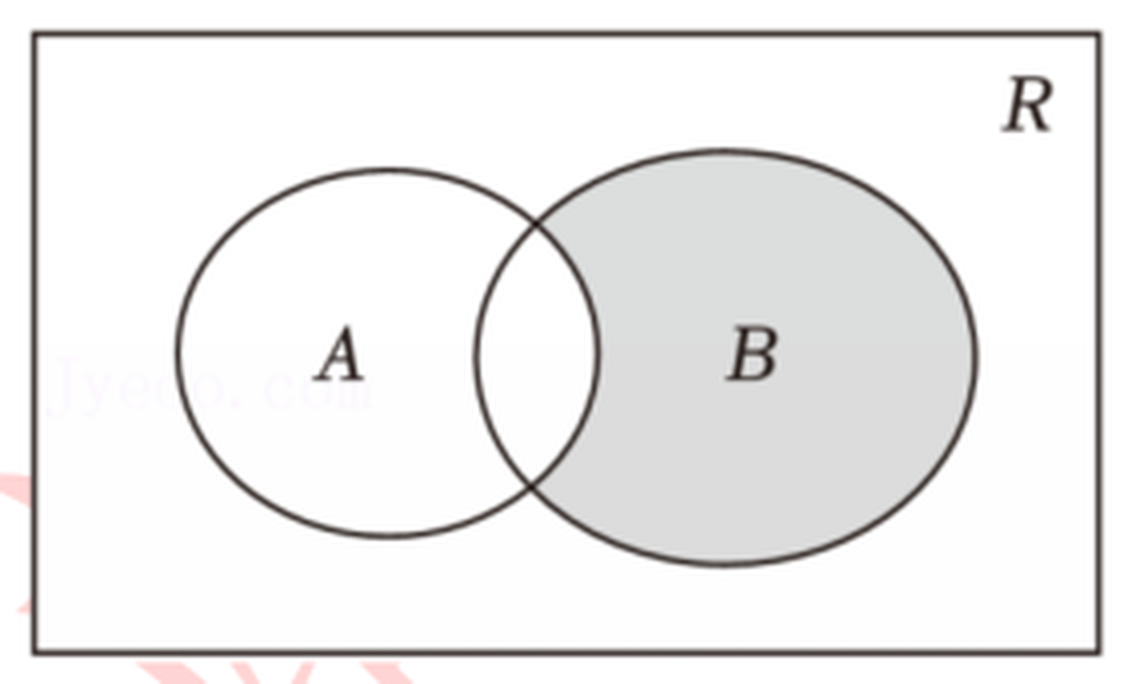
\includegraphics[width=0.30\textwidth]{figures/venn_Abar_cap_B.png}
\end{center}

\begin{enumerate}[label=(\arabic*)]
\item 若 $a=1$，求阴影部分表示的集合.
\item 若 $A\cap B=B$，求实数 $a$ 的取值范围.
\end{enumerate}

\ifanswer
\solbegin
\stepm{(1)}{因为 $\dfrac{2x-3}{x+5}\leqslant0$，
等价于 $\begin{cases}(2x-3)(x+5)\leqslant0\\ x+5\neq0\end{cases}$，}
\step{解得 $-5<x\leqslant\dfrac32$，即 $A=\left\{x\mid-5<x\leqslant\dfrac32\right\}$；}
\step{若 $a=1$，因为 $|x-1|<1$，等价于 $-1<x-1<1$，}
\step{解得 $0<x<2$，即 $B=\{x\mid0<x<2\}$.}
\step{由 Venn 图得阴影部分表示的集合为 $\overline{A}\cap B=\left(\dfrac32,2\right)$.}
\stepm{(2)}{由 (1) 得 $A=\left\{x\mid-5<x\leqslant\dfrac32\right\}$，}
\step{$B=\{x\mid|x-a|<1\}=\{x\mid-1+a<x<1+a\}\neq\varnothing$，}
\step{因为 $A\cap B=B$，所以 $B\sub A$，}
\step{所以 $\begin{cases}-5\leqslant-1+a\\ 1+a\leqslant\dfrac32\end{cases}$，
解得 $-4\leqslant a\leqslant\dfrac12$，}
\step{所以实数 $a$ 的取值范围为 $\left[-4,\dfrac12\right]$.}
\solend

\fi

\ansspace[6]

\item 设 $A=\{x\mid x^2-(m+3)x+2(m+1)=0,m\in\R\}$，
$B=\{x\mid 2x^2+(3n+1)x+2=0,n\in\R\}$.

\begin{enumerate}[label=(\arabic*)]
\item 是否存在 $m$、$n\in\R$，使得 $A=\{1,2\}$，$B=\varnothing$，说明理由；
\item 若 $A\cap B=A$，求 $m$、$n$ 的值.
\end{enumerate}

\ifanswer
\solbegin
\stepm{(1)}{由 $A=\{1,2\}$，得 $m=0$，}
\step{再由 $B=\varnothing$，得 $\Delta=(3n+1)^2-4\times2\times2=9n^2+6n-15<0$，}
\step{所以 $(3n+5)(n-1)<0$，解得 $-\dfrac53<n<1$，}
\step{故存在 $m=0$，$-\dfrac53<n<1$，使得 $A=\{1,2\}$，$B=\varnothing$.}
\stepm{(2)}{由 $x^2-(m+3)x+2(m+1)=0$，得 $x=2$ 或 $x=m+1$，}
\step{若 $A\cap B=A$，则 $A\sub B$，}
\step{将 $x=2$ 代入 $2x^2+(3n+1)x+2=0$，得 $n=-2$，}
\step{则 $B=\{x\mid 2x^2+(3n+1)x+2=0,n\in\R\}=\{x\mid 2x^2-5x+2=0\}
=\left\{2,\dfrac12\right\}$.}
\step{则 $m+1=\dfrac12$ 或 $m+1=2$，则 $m=-\dfrac12$ 或 $m=1$，
所以 $m=-\dfrac12$ 或 $m=1$，$n=-2$.}
\solend

\fi

\ansspace[6]

\item 已知陈述句 $\alpha$：关于 $x$ 的方程 $x^2-6x+m=0$ 有两个不同的正数根，陈述句
$\beta$：集合 $\{x\mid(m+1)x^2+4x+1=0,x\in\R\}$ 中至多有一个元素.

\begin{enumerate}[label=(\arabic*)]
\item 若 $\alpha$ 和 $\beta$ 都是真命题，求实数 $m$ 的取值范围；
\item 若 $\alpha$ 和 $\beta$ 至多有一个是假命题，求实数 $m$ 的取值范围.
\end{enumerate}

\ifanswer
\solbegin
\stepm{(1)}{因为关于 $x$ 的方程 $x^2-6x+m=0$ 有两个不同的正数根，}
\step{则 $\begin{cases}36-4m>0\\ m>0\end{cases}$，解得 $0<m<9$，}
\step{集合 $\{x\mid(m+1)x^2+4x+1=0,x\in\R\}$ 中至多有一个元素，}
\step{则 $m=-1$ 或 $\begin{cases}m+1\neq0\\ 16-4(m+1)\leqslant0\end{cases}$，
解得 $m\geqslant3$，}
\step{$\alpha$ 和 $\beta$ 都是真命题，所以实数 $m$ 的取值范围为 $\{m\mid3\leqslant m<9\}$}
\stepm{(2)}{由 (1) 得当 $\alpha$ 为假命题时，$m\leqslant0$ 或 $m\geqslant9$，}
\step{当 $\beta$ 为假命题时，$m<3$ 且 $m\neq-1$，}
\step{所以 $\alpha$ 和 $\beta$ 均为假命题时，$m$ 的范围是 $m\leqslant0$ 且 $m\neq-1$，}
\step{$\alpha$ 和 $\beta$ 至多有一个是假命题时，实数 $m$ 的取值范围为
$\{m\mid m>0$ 或 $m=-1\}$.}
\solend

\fi

\ansspace[6]

\item 已知符号 $[x]$ 表示不大于 $x$ 的最大整数 $(x\in\R)$，例如：$[1.3]=1$，
$[2]=2$，$[-1.2]=-2$.

\begin{enumerate}[label=(\arabic*)]
\item 已知方程 $[x]=3$，求该方程的解集；
\item 设方程 $\bigl[|x|+|x-1|\bigr]=3$ 的解集为 $A$，
集合 $B=\{x\mid 2x^2-11kx+15k^2\geqslant0\}$，若 $A\cup B=\R$，求实数 $k$ 的取值范围；
\item 在 (2) 的条件下，集合 $C=\{x\mid x^2-ax+1-2a\leqslant0,a\in\R\}$，是否存在实数
$a$，$A\cap C=A$，若存在，请求出实数 $a$ 的取值范围；若不存在，请说明理由.
\end{enumerate}

\ifanswer
\solbegin
\stepm{(1)}{方程 $[x]=3$，则 $x\in[3,4)$，所以该方程的解集为 $[3,4)$；}
\stepm{(2)}{因为 $\bigl[|x|+|x-1|\bigr]=3$，所以 $3\leqslant|x|+|x-1|<4$，}
\step{由绝对值不等式的几何意义得 $A=\left(-\dfrac32,-1\right]\cup\left[2,\dfrac52\right)$，}
\step{又 $B=\{x\mid 2x^2-11kx+15k^2\geqslant0\}=\{x\mid(2x-5k)(x-k)\geqslant0\}$，}
\step{当 $k=0$ 时，$B=\{x\mid 2x^2\geqslant0\}=\R$，则 $A\cup B=\R$，符合题意；}
\step{当 $k>0$ 时，$B=\left(-\infty,\dfrac{5k}{2}\right]\cup[3k,+\infty)$，
若 $A\cup B=\R$，}
\step{则 $\begin{cases}\dfrac{5k}{2}\geqslant2\\[2pt] 3k\leqslant\dfrac52\end{cases}$，
解得 $k\in\left[\dfrac45,\dfrac56\right]$；}
\step{当 $k<0$ 时，$B=(-\infty,3k]\cup\left[\dfrac{5k}{2},+\infty\right)$，
若 $A\cup B=\R$，}
\step{则 $\begin{cases}\dfrac{5k}{2}\leqslant-1\\[2pt] 3k\geqslant-\dfrac32\end{cases}$，
解得 $k\in\left[-\dfrac12,-\dfrac25\right]$.}
\step{综上所述，实数 $k$ 的取值范围为
$\left[-\dfrac12,-\dfrac25\right]\cup\{0\}\cup\left[\dfrac45,\dfrac56\right]$；}
\stepm{(3)}{因为 $A\cap C=A$，则 $A\sub C$ 且
$A=\left(-\dfrac32,-1\right]\cup\left[2,\dfrac52\right)$，}
\step{设集合 $C$ 的解集为 $(x_1,x_2)(x_1<x_2)$，}
\step{则 $\begin{cases}x_1\leqslant-\dfrac32\\[2pt] x_2\geqslant\dfrac52\end{cases}$，}
\step{所以
$\begin{cases}\Delta=a^2-4(1-2a)>0\\[2pt]
f\!\left(-\dfrac32\right)=\dfrac94+\dfrac32a+1-2a\leqslant0\\[4pt]
f\!\left(\dfrac52\right)=\dfrac{25}{4}-\dfrac52a+1-2a\leqslant0\end{cases}$，
解得 $a\geqslant\dfrac{13}{2}$，}
\step{故实数 $a$ 的取值范围为 $\left[\dfrac{13}{2},+\infty\right)$.}
\solend

\fi

\ansspace[6]

\item 非空有限集合 $S$ 是由若干个正实数组成，集合 $S$ 的元素个数不少于 $2$ 个. 对于任意
$a,b\in S,a\neq b$，若数 $a^b$ 或 $b^a$ 中至少有一个属于 $S$，则称集合 $S$ 是“好集”；
否则，称集合 $S$ 是“坏集”.

\begin{enumerate}[label=(\arabic*)]
\item 判断 $A=\{1,3,9\}$ 和 $B=\left\{1,\dfrac12,\dfrac14,\dfrac1{16}\right\}$ 是“好集”
还是“坏集”，并简单说明理由；
\item 题设的有限集 $S$ 中，既有大于 $1$ 的元素，又有小于 $1$ 的元素，证明：集合 $S$ 是
“坏集”；
\item 若题设中的 $a^b$ 或 $b^a$ 都属于 $S$，则称集合 $S$ 为“超级好集”，写出一个
“超级好集”（无须证明）.
\end{enumerate}

\ifanswer
\solbegin
\stepm{(1)}{$A=\{1,3,9\}$，$3^9\notin A$，$9^3\notin A$，所以 $A$ 是“坏集”，}
\step{从 $B$ 集合中任意取两个数字都满足需求，所以 $B$ 是“好集”.}
\stepm{(2)}{假设 $a$ 是 $S$ 中小于 $1$ 的元素中的最小元素，}
\step{$b$ 是 $S$ 中大于 $1$ 的元素中的最小元素，则 $a^b<a^1=a$，}
\step{所以 $a$ 就不是 $S$ 中小于 $1$ 的元素中的最小元素，即 $a^b\notin S$，}
\step{同理 $1=b^0<b^a<b^1=b$，所以 $b$ 就不是 $S$ 中大于 $1$ 的元素中的最小元素，}
\step{即 $b^a\notin S$，所以集合 $S$ 是“坏集”；}
\stepm{(3)}{首先 $S=\{1,a\}$（$a\neq1$ 且 $a>0$）是“超级好集”，}
\step{假设 $0<a<1$，由 (2) 得，$S$ 中不可能有大于 $1$ 的元素，}
\step{假设 $S$ 中有除 $a$ 之外的元素 $b\in S$（$a\neq b,b<1$），}
\step{假设 $a$ 是 $S$ 中小于 $1$ 的元素中的最大元素，$a^b>a^1=a$，}
\step{所以 $a$ 不是最大元素，所以 $a^b\notin S$，所以 $b\notin S$；}
\step{假设 $a>1$，由 (2) 得 $S$ 中不可能有小于 $1$ 的元素，}
\step{假设 $S$ 中有除 $a$ 之外的元素 $b$（$b>1$ 且 $b\neq a$），}
\step{假设 $a$ 是 $S$ 中大于 $1$ 的元素中的最小元素，则 $a^b>a^1=a$，}
\step{所以 $a$ 不是最小元素，即不存在 $b>1$，使得 $b\in S$，即 $b\notin S$，}
\step{综上，$S=\{1,a\}$（$a\neq1$ 且 $a>0$）.}
\solend

\fi

\ansspace*[10]

\end{enumerate}

\end{document}
"
%
% 原始材料是微信公众号图文（公众号「魔都数学加油站」连载「27学年高一 25」，2026-09-21 发布，
% 原文标题「27学年高一25——2026-2027年上海市华师大二附中高一上周末作业3」），
% 正文为 10 张 PNG 页（1080×1527，各页同尺寸）。原文本身就是一份**讲评版**——
% 题目下方直接印出【解析】（本卷无单独的【答案】行，填空题答案都写在解析里）。
% 试题文字与解析均照原卷录入，未改内容。卷面的粉色斜水印「魔都数学加油站」属水印，未录入。
%
% 卷首标题：原卷印作「2026-2027 年华师大二附中高一上周末作业 3」（公众号标题里的「上海市」
% 三字卷面标题行没有，本稿照卷面），年份区间按全稿惯例排 en dash，前缀照原卷保留「年」。
%
% 与原卷的排版差异（均已在 README「说明」中交代）：
%   ① 原文自**第 3 题**起（第 1、2 题未在该文中发布），故本稿题号亦自 3 起；
%   ② 原卷本就印有「一、填空题」「二、选择题」「三、解答题」三节标题，本稿照原卷分节，
%      只把标题改排成全稿统一的「大节标题」样式；
%   ③ 原卷第 13 题的答案「D」直接印在题干末尾的括号内，第 14—16 题的括号空着、答案写在
%      解析末句「故选 C／B」里；填空题的答案也都嵌在解析里，本稿统一改为试卷版隐去、
%      答案版以 \ans{} 给出（选择题另附【解析】），使两版彻底分离；
%   ④ 补集符号原卷一律作**上横线**（$\overline{A}$、$\overline{A\cup B}$），与同校的
%      高一14 同例，本稿照录（不改为 $\complement_U A$ 写法）；
%   ⑤ 原卷的实数集 R 斜体与粗体混用（第 17 题题干「全集为 R」作粗体，第 5、14 题与
%      第 16 题解析的 $R$ 为斜体），本稿按全稿惯例统一写作 $\R$；
%   ⑥ 原卷填空的横线约两个字宽，本稿按全稿惯例统一排 \blankline[4.4em]；
%   ⑦ 原卷未印副标题，本稿按全稿惯例补出副标题「集合与常用逻辑用语」；
%   ⑧ 第 17 题的 Venn 图原卷印在题干右侧（第 6 页），本稿移至题干之后；
%      图取原卷截图、4× LANCZOS 放大（figures/venn_Abar_cap_B.png，
%      阴影为 $B$ 中不含 $A\cap B$ 的部分，即 $\overline{A}\cap B$）。
%
% 原卷存疑两处（均照抄原卷、未改，见源码中该处上方注释）：
%   ① 第 8 题【解析】第二段「当 $\Delta=a^2-16>0$ 时，方程 $x^2+ax+4=0$ 有两个相同的根
%      $x_1$、$x_2$」——$\Delta>0$ 应为「两个**不**相同的根」（其自己的后文就把 $x_1$、$x_2$
%      当作可以不同的两个根在讨论），显系笔误；
%   ② 第 11 题【解析】先写「偶数必是 $2^{11}\cdot3^m\cdot337^n$，$m$、$n\in\N^*$」，
%      下一行又写「$0\leqslant m\leqslant10$，$0\leqslant n\leqslant10$，共有 121 种情况」
%      ——按 $\N^*$ 应从 1 起（至多 $10\times10=100$ 种），与 121（$=11\times11$，含 0）
%      对不上，两处至少有一处笔误。

\documentclass[a4paper,11pt]{article}
\usepackage{common}

\begin{document}

\examtitlest[3]{2026--2027 年华师大二附中高一上周末作业 3}{集合与常用逻辑用语}

\bigsec{一、填空题}

\begin{enumerate}
\setcounter{enumi}{2}

\item 设全集 $U=\{2,4,m^2+m-5\}$，集合 $A=\{2,1-m\}$，若 $\overline{A}=\{1\}$，则实数
$m=$ \blankline[4.4em].

\ifanswer
\solbegin
\step{因为 $\overline{A}=\{1\}$，所以 $1\in U$，$1\notin A$，}
\step{所以 $\begin{cases}m^2+m-5=1\\ 1-m\neq1\\ 1-m=4\end{cases}$，解得 $m=-3$.}
\solend

\fi

\item 已知条件 $\alpha$：$m<x\leqslant2m+5$，条件 $\beta$：$0\leqslant x\leqslant1$，
若 $\alpha$ 是 $\beta$ 的必要条件，则实数 $m$ 的取值范围为 \blankline[4.4em].

\ifanswer
\solbegin
\step{若 $\alpha$ 是 $\beta$ 的必要条件，则 $[0,1]\sub(m,2m+5]$，}
\step{所以 $\begin{cases}m<2m+5\\ m<0\\ 2m+5\geqslant1\end{cases}$，}
\step{解得 $-2\leqslant m<0$，故实数 $m$ 的取值范围为 $[-2,0)$.}
\solend

\fi

\item 已知 $\R$ 是全集，集合 $A=\{y\mid y=-x^2+1,x\in\R\}$，集合
$B=\{x\mid x=3+|a|,a\in\R\}$，则 $\overline{A\cup B}=$ \blankline[4.4em].

\ifanswer
\solbegin
\step{$A=\{y\mid y=-x^2+1,x\in\R\}=(-\infty,1]$，}
\step{$B=\{x\mid x=3+|a|,a\in\R\}=[3,+\infty)$，}
\step{所以 $\overline{A\cup B}=(1,3)$.}
\solend

\fi

\item 已知 $a$ 为常数，集合 $A=\{x\mid x^2+x-6=0\}$，集合 $B=\{x\mid ax-2=0\}$，且
$B\sub A$，则 $a$ 的所有取值构成的集合为 \blankline[4.4em].

\ifanswer
\solbegin
\step{集合 $A=\{-3,2\}$，因为 $B\sub A$，所以 $B=\varnothing$，$\{-3\}$，$\{2\}$，$\{-3,2\}$，}
\step{当 $B=\varnothing$ 时，$a=0$，当 $B=\{-3\}$ 时，$a=-\dfrac23$，当 $B=\{2\}$ 时，$a=1$，}
\step{当 $B=\{-3,2\}$ 时，不成立，故 $a$ 的取值集合为 $\left\{0,-\dfrac23,1\right\}$.}
\solend

\fi

\item 已知一元二次方程 $x^2+px+p=0$ 有两个不相等的实根分别为 $x_1$、$x_2$.
$A=x_1^2+x_2^2$，$B=x_1x_2(x_1+x_2)$，$A$ 与 $B$ 的大小为 \blankline[4.4em].

\ifanswer
\solbegin
\step{一元二次方程 $x^2+px+p=0$ 有两个不相等的实根分别为 $x_1$、$x_2$，}
\step{则 $\Delta=p^2-4p>0$，解得 $p<0$ 或 $p>4$，}
\step{由韦达定理得 $x_1+x_2=-p$，$x_1x_2=p$，}
\step{所以 $A=x_1^2+x_2^2=(x_1+x_2)^2-2x_1x_2=p^2-2p$，$B=x_1x_2(x_1+x_2)=-p^2$，}
\step{所以 $A-B=(p^2-2p)-(-p^2)=2p(p-1)$，}
\step{当 $p<0$ 时，则 $A-B>0$，故 $A>B$，}
\step{当 $p>4$ 时，则 $A-B>0$，故 $A>B$，}
\step{综上，$A=p^2-2p$，$B=-p^2$，且 $A>B$.}
\solend

\fi

\item 集合 $A=\{x\mid(x-1)(x^2+ax+4)=0,x\in\R\}$ 中所有元素之和为 $3$，则实数
$a=$ \blankline[4.4em].

\ifanswer
\solbegin
\step{当 $\Delta=a^2-16=0$ 时，方程 $x^2+ax+4=0$ 有两个相同的根 $-\dfrac a2$，}
\step{则 $A=\left\{1,-\dfrac a2\right\}$，故 $1-\dfrac a2=3$，解得 $a=-4$；}
% 注：下一行的「两个相同的根」系原卷笔误（△>0 应为「两个不相同的根」，其自己的后文
%     就把 x₁、x₂ 当作可以不同的两个根在讨论），照抄原卷、未改，见文件头「原卷存疑」①。
\step{当 $\Delta=a^2-16>0$ 时，方程 $x^2+ax+4=0$ 有两个相同的根 $x_1$、$x_2$，}
\step{若 $1$ 是方程 $x^2+ax+4=0$ 的根，则方程 $x^2+ax+4=0$ 的另一个根为 $4$，}
\step{则 $A=\{1,4\}$，不成立；}
\step{若 $1$ 不是方程 $x^2+ax+4=0$ 的根，则 $A=\{1,x_1,x_2\}$，则 $1+x_1+x_2=3$，}
\step{故 $x_1+x_2=2=-a$，故 $a=-2$（舍去）；}
\step{综上所述，$a=-4$.}
\solend

\fi

\item 已知集合 $A=\{x\mid x^2+2x-8\geqslant0\}$，$B=\{x\mid x^2-2ax+4\leqslant0\}$，
若 $a>0$，且 $A\cap B\cap\N$ 中恰有 $2$ 个元素，则 $a$ 的取值范围为 \blankline[4.4em].

\ifanswer
\solbegin
\step{由 $A$ 中不等式变形得 $(x-2)(x+4)\geqslant0$，解得 $x\leqslant-4$ 或 $x\geqslant2$，}
\step{即 $A=(-\infty,-4]\cup[2,+\infty)$，}
\step{设 $f(x)=x^2-2ax+4$，则 $f(x)$ 的轴对称 $x=a>0$，}
\step{且对应方程的根 $x_1$、$x_2$ 满足 $\begin{cases}x_1x_2=4\\ x_1+x_2>0\end{cases}$，}
\step{所以 $0<x_1\leqslant2\leqslant x_2$（取 $x_1\leqslant x_2$），}
\step{所以 $A\cap B\cap\N$ 中恰有的整数为 $2$，$3$，}
\step{所以 $\begin{cases}f(3)=9-6a+4\leqslant0\\ f(4)=16-8a+4>0\end{cases}$，}
\step{解得 $\dfrac{13}{6}\leqslant a<\dfrac52$，所以 $a$ 的取值范围为 $\left[\dfrac{13}{6},\dfrac52\right)$.}
\solend

\fi

\item 在三个关于 $x$ 的方程 $x^2-ax+4=0$，$x^2+(a-1)x+16=0$ 和
$x^2+2ax+3a+10=0$ 中至少有一个方程有实根，则实数 $a$ 的取值范围是 \blankline[4.4em].

\ifanswer
\solbegin
\step{当三个方程均无实根时，有}
\step{$\begin{cases}\Delta_1=a^2-16<0\\ \Delta_2=(a-1)^2-64<0\\ \Delta_3=4a^2-4(3a+10)<0\end{cases}$，}
\step{所以 $\begin{cases}-4<a<4\\ -7<a<9\\ -2<a<5\end{cases}$，}
\step{所以 $-2<a<4$，故三个方程均无实根时，$a$ 的取值范围为 $(-2,4)$，}
\step{所以三个方程中至少有一个方程有实根时，}
\step{实数 $a$ 的取值范围为 $(-\infty,-2]\cup[4,+\infty)$.}
\solend

\fi

% 注：下一行解析里的「m、n∈N*」与再下一行的「0≤m≤10，0≤n≤10，共有 121 种情况」
%     对不上（按 N* 应从 1 起，至多 10×10=100 种；121=11×11 含 0），系原卷自身矛盾，
%     照抄原卷、未改，见文件头「原卷存疑」②。
\item 若集合 $M=\{(x,y)\mid(x+1)+(x+2)+\cdots+(x+y)=2022^{10},x\in\Z,y\in\N^{*}\}$，
则集合 $M$ 中元素有 \blankline[4.4em] 个.

\ifanswer
\solbegin
\step{由题意得 $(x+1)+(x+2)+\cdots+(x+y)=\dfrac{y(2x+1+y)}{2}$，}
\step{所以 $y(2x+1+y)=2^{11}\cdot3^{10}\cdot337^{10}$，}
\step{因为 $y$ 与 $2x+1+y$ 必为一奇一偶，偶数必是 $2^{11}\cdot3^m\cdot337^n$，
$m$、$n\in\N^{*}$，}
\step{$0\leqslant m\leqslant10$，$0\leqslant n\leqslant10$，共有 $121$ 种情况，}
\step{因为 $y$ 与 $2x+1+y$ 奇偶未定，所以集合 $M$ 中元素只有 $242$ 个.}
\solend

\fi

\item 设集合 $M=\left\{x\mid m\leqslant x\leqslant m+\dfrac34\right\}$，
$N=\left\{x\mid n-\dfrac13\leqslant x\leqslant n\right\}$，且 $M$、$N$ 都是集合
$\{x\mid0\leqslant x\leqslant1\}$ 的子集，如果把 $b-a$ 叫做集合
$\{x\mid a\leqslant x\leqslant b\}$ 的长度，那么集合 $M\cap N$ 的长度的最小值是
\blankline[4.4em].

\ifanswer
\solbegin
\step{$M$ 的长度为 $\dfrac34$，$N$ 的长度为 $\dfrac13$，}
\step{当集合 $M\cap N$ 的长度的最小值时，$M$ 与 $N$ 应分别在区间 $[0,1]$ 的左右两端，}
\step{故 $M\cap N$ 的长度的最小值是 $\dfrac34+\dfrac13-1=\dfrac1{12}$.}
\solend

\fi

\end{enumerate}

\bigsec{二、选择题}

\begin{enumerate}
\setcounter{enumi}{12}

\item 直角坐标平面中除去两点 $A(1,1)$、$B(2,-2)$ 可用集合表示为\mbox{（\quad）}

\keepwithprev
A. $\{(x,y)\mid x\neq1,y\neq1,x\neq2,y\neq-2$\}\qquad
B. $\{(x,y)\mid\begin{cases}x\neq1\\ y\neq1\end{cases}$ 或 $\begin{cases}x\neq2\\ y\neq-2\end{cases}\}$

C. $\{(x,y)\mid[(x-1)^2+(y-1)^2][(x-2)^2+(y+2)^2]\neq0$\}

D. $\{(x,y)\mid[(x-1)^2+(y-1)^2]+[(x-2)^2+(y+2)^2]\neq0$\}

\ans{$D$}

\item 已知函数 $f(x)=x^2+nx$，记集合 $A=\{x\mid f(x)=0,x\in\R\}$，
$B=\{x\mid f(f(x))=0,x\in\R\}$，若 $A=B\neq\varnothing$，则 $n$ 的取值范围是\mbox{（\quad）}

\keepwithprev
A. $[0,4]$\qquad B. $(0,4)$\qquad C. $[0,4)$\qquad D. $(0,4]$

\ans{$C$}

\ifanswer
\solbegin
\step{$f(x)=x^2+nx$，$f[f(x)]=(x^2+nx)^2+n(x^2+nx)=(x^2+nx)(x^2+nx+n)$，}
\step{当 $n=0$ 时，$f(x)=x^2$，$f[f(x)]=x^4$，满足 $A=B$，此时 $n=0$；}
\step{当 $n\neq0$ 时，$0$、$-n$ 不是 $x^2+nx+n=0$ 的根，故 $\Delta=n^2-4n<0$，
解得 $0<n<4$，}
\step{综上所述，$n$ 的取值范围是 $[0,4)$. 故选 $C$.}
\solend

\fi

\item 设全集 $U=\{1,2,3,4,5,6,7,8,9,10\}$，给出条件：① $A\sub U$；②若 $x\in A$，
则 $2x\notin A$；③若 $x\in\overline{A}$，则 $2x\notin\overline{A}$.
那么同时满足三个条件的集合 $A$ 的个数为\mbox{（\quad）}

\keepwithprev
A. $0$ 个\qquad B. $16$ 个\qquad C. $32$ 个\qquad D. $64$ 个

\ans{$C$}

\ifanswer
\solbegin
\step{由① $A\sub U$；②若 $x\in A$，则 $2x\notin A$；③若 $x\in\overline{A}$，
则 $2x\notin\overline{A}$.}
\step{若 $1\in A$，则 $2\notin A$，即 $2\in\overline{A}$，则 $4\notin\overline{A}$，
即 $4\in A$，则 $8\notin A$，即 $8\in\overline{A}$；}
\step{若 $3\in A$，则 $6\notin A$，即 $6\in\overline{A}$；若 $5\in A$，则 $10\notin A$，
即 $10\in\overline{A}$，}
\step{故 $1$、$4$ 和 $2$、$8$ 分开，$3$ 和 $6$ 分开，$5$ 和 $10$ 分开，$7$ 和 $9$ 随意，}
\step{故同时满足三个条件的集合 $A$ 的个数为 $2\times2\times2\times2\times2=32$，
故选 $C$.}
\solend

\fi

\item 设集合 $P_1=\{x\mid x^2+ax+1>0\}$，$P_2=\{x\mid x^2+ax+2>0\}$，
$Q_1=\{x\mid x^2+x+b>0\}$，$Q_2=\{x\mid x^2+2x+b>0\}$，其中 $a$、$b\in\R$，
下列说法中正确的是\mbox{（\quad）}

\keepwithprev
A. 对任意 $a$，$P_1$ 是 $P_2$ 的子集，对任意的 $b$，$Q_1$ 不是 $Q_2$ 的子集

B. 对任意 $a$，$P_1$ 是 $P_2$ 的子集，存在 $b$，使得 $Q_1$ 是 $Q_2$ 的子集

C. 存在 $a$，使得 $P_1$ 不是 $P_2$ 的子集，对任意的 $b$，$Q_1$ 不是 $Q_2$ 的子集

D. 存在 $a$，使得 $P_1$ 不是 $P_2$ 的子集，存在 $b$，使得 $Q_1$ 是 $Q_2$ 的子集

\ans{$B$}

\ifanswer
\solbegin
\step{对于集合 $P_1=\{x\mid x^2+ax+1>0\}$，$P_2=\{x\mid x^2+ax+2>0\}$，}
\step{得当 $m\in P_1$ 时，即 $m^2+am+1>0$，得 $m^2+am+2>0$，}
\step{即有 $m\in P_2$，得对任意 $a$，$P_1$ 是 $P_2$ 的子集，}
\step{对于集合 $Q_1=\{x\mid x^2+x+b>0\}$，$Q_2=\{x\mid x^2+2x+b>0\}$，}
\step{当 $b=6$ 时，$Q_1=\{x\mid x^2+x+6>0\}=\R$，$Q_2=\{x\mid x^2+2x+6>0\}=\R$，}
\step{得 $Q_1$ 是 $Q_2$ 的子集，}
\step{当 $b=1$ 时，$Q_1=\{x\mid x^2+x+1>0\}=\R$，}
\step{$Q_2=\{x\mid x^2+2x+1>0\}=\{x\mid x\neq-1\}$，得 $Q_1$ 不是 $Q_2$ 的子集，}
\step{所以存在 $b$，使得 $Q_1$ 是 $Q_2$ 的子集，故选 $B$.}
\solend

\fi

\end{enumerate}

\bigsec{三、解答题}

\begin{enumerate}
\setcounter{enumi}{16}

\item 已知集合 $A=\left\{x\mid\dfrac{2x-3}{x+5}\leqslant0\right\}$，
$B=\{x\mid|x-a|<1\}$，全集为 $\R$.

\begin{center}
% 图取原卷截图、4× LANCZOS 放大（原卷把图印在题干右侧，本稿移至此处，见文件头⑧）。
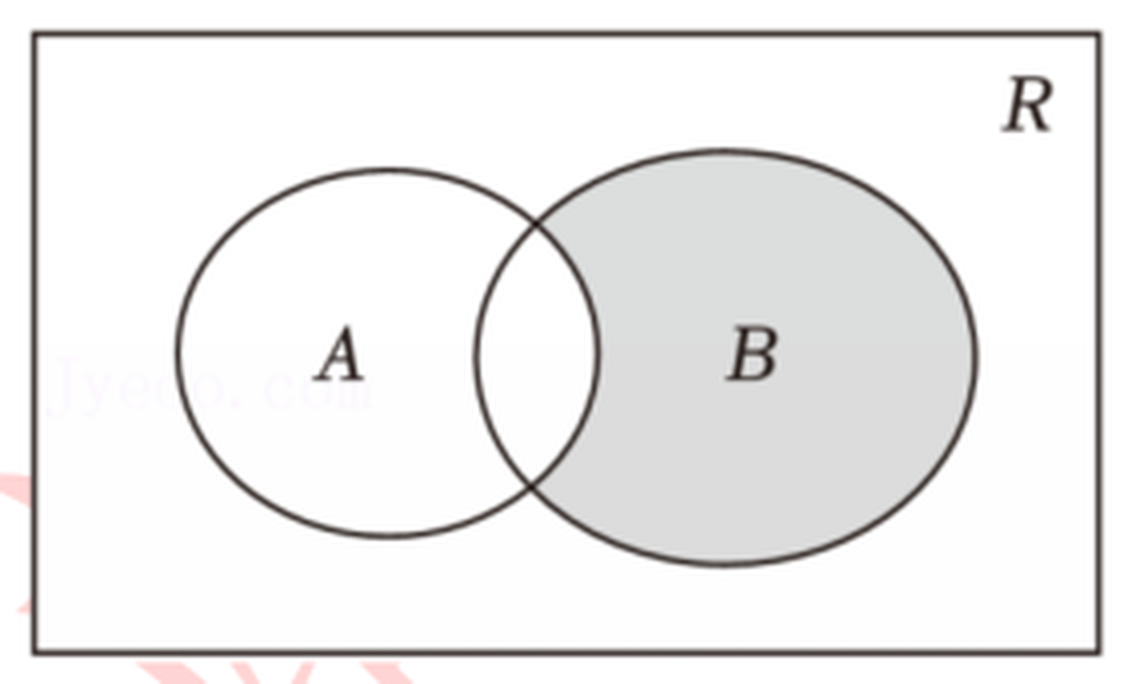
\includegraphics[width=0.30\textwidth]{figures/venn_Abar_cap_B.png}
\end{center}

\begin{enumerate}[label=(\arabic*)]
\item 若 $a=1$，求阴影部分表示的集合.
\item 若 $A\cap B=B$，求实数 $a$ 的取值范围.
\end{enumerate}

\ifanswer
\solbegin
\stepm{(1)}{因为 $\dfrac{2x-3}{x+5}\leqslant0$，
等价于 $\begin{cases}(2x-3)(x+5)\leqslant0\\ x+5\neq0\end{cases}$，}
\step{解得 $-5<x\leqslant\dfrac32$，即 $A=\left\{x\mid-5<x\leqslant\dfrac32\right\}$；}
\step{若 $a=1$，因为 $|x-1|<1$，等价于 $-1<x-1<1$，}
\step{解得 $0<x<2$，即 $B=\{x\mid0<x<2\}$.}
\step{由 Venn 图得阴影部分表示的集合为 $\overline{A}\cap B=\left(\dfrac32,2\right)$.}
\stepm{(2)}{由 (1) 得 $A=\left\{x\mid-5<x\leqslant\dfrac32\right\}$，}
\step{$B=\{x\mid|x-a|<1\}=\{x\mid-1+a<x<1+a\}\neq\varnothing$，}
\step{因为 $A\cap B=B$，所以 $B\sub A$，}
\step{所以 $\begin{cases}-5\leqslant-1+a\\ 1+a\leqslant\dfrac32\end{cases}$，
解得 $-4\leqslant a\leqslant\dfrac12$，}
\step{所以实数 $a$ 的取值范围为 $\left[-4,\dfrac12\right]$.}
\solend

\fi

\ansspace[6]

\item 设 $A=\{x\mid x^2-(m+3)x+2(m+1)=0,m\in\R\}$，
$B=\{x\mid 2x^2+(3n+1)x+2=0,n\in\R\}$.

\begin{enumerate}[label=(\arabic*)]
\item 是否存在 $m$、$n\in\R$，使得 $A=\{1,2\}$，$B=\varnothing$，说明理由；
\item 若 $A\cap B=A$，求 $m$、$n$ 的值.
\end{enumerate}

\ifanswer
\solbegin
\stepm{(1)}{由 $A=\{1,2\}$，得 $m=0$，}
\step{再由 $B=\varnothing$，得 $\Delta=(3n+1)^2-4\times2\times2=9n^2+6n-15<0$，}
\step{所以 $(3n+5)(n-1)<0$，解得 $-\dfrac53<n<1$，}
\step{故存在 $m=0$，$-\dfrac53<n<1$，使得 $A=\{1,2\}$，$B=\varnothing$.}
\stepm{(2)}{由 $x^2-(m+3)x+2(m+1)=0$，得 $x=2$ 或 $x=m+1$，}
\step{若 $A\cap B=A$，则 $A\sub B$，}
\step{将 $x=2$ 代入 $2x^2+(3n+1)x+2=0$，得 $n=-2$，}
\step{则 $B=\{x\mid 2x^2+(3n+1)x+2=0,n\in\R\}=\{x\mid 2x^2-5x+2=0\}
=\left\{2,\dfrac12\right\}$.}
\step{则 $m+1=\dfrac12$ 或 $m+1=2$，则 $m=-\dfrac12$ 或 $m=1$，
所以 $m=-\dfrac12$ 或 $m=1$，$n=-2$.}
\solend

\fi

\ansspace[6]

\item 已知陈述句 $\alpha$：关于 $x$ 的方程 $x^2-6x+m=0$ 有两个不同的正数根，陈述句
$\beta$：集合 $\{x\mid(m+1)x^2+4x+1=0,x\in\R\}$ 中至多有一个元素.

\begin{enumerate}[label=(\arabic*)]
\item 若 $\alpha$ 和 $\beta$ 都是真命题，求实数 $m$ 的取值范围；
\item 若 $\alpha$ 和 $\beta$ 至多有一个是假命题，求实数 $m$ 的取值范围.
\end{enumerate}

\ifanswer
\solbegin
\stepm{(1)}{因为关于 $x$ 的方程 $x^2-6x+m=0$ 有两个不同的正数根，}
\step{则 $\begin{cases}36-4m>0\\ m>0\end{cases}$，解得 $0<m<9$，}
\step{集合 $\{x\mid(m+1)x^2+4x+1=0,x\in\R\}$ 中至多有一个元素，}
\step{则 $m=-1$ 或 $\begin{cases}m+1\neq0\\ 16-4(m+1)\leqslant0\end{cases}$，
解得 $m\geqslant3$，}
\step{$\alpha$ 和 $\beta$ 都是真命题，所以实数 $m$ 的取值范围为 $\{m\mid3\leqslant m<9\}$}
\stepm{(2)}{由 (1) 得当 $\alpha$ 为假命题时，$m\leqslant0$ 或 $m\geqslant9$，}
\step{当 $\beta$ 为假命题时，$m<3$ 且 $m\neq-1$，}
\step{所以 $\alpha$ 和 $\beta$ 均为假命题时，$m$ 的范围是 $m\leqslant0$ 且 $m\neq-1$，}
\step{$\alpha$ 和 $\beta$ 至多有一个是假命题时，实数 $m$ 的取值范围为
$\{m\mid m>0$ 或 $m=-1\}$.}
\solend

\fi

\ansspace[6]

\item 已知符号 $[x]$ 表示不大于 $x$ 的最大整数 $(x\in\R)$，例如：$[1.3]=1$，
$[2]=2$，$[-1.2]=-2$.

\begin{enumerate}[label=(\arabic*)]
\item 已知方程 $[x]=3$，求该方程的解集；
\item 设方程 $\bigl[|x|+|x-1|\bigr]=3$ 的解集为 $A$，
集合 $B=\{x\mid 2x^2-11kx+15k^2\geqslant0\}$，若 $A\cup B=\R$，求实数 $k$ 的取值范围；
\item 在 (2) 的条件下，集合 $C=\{x\mid x^2-ax+1-2a\leqslant0,a\in\R\}$，是否存在实数
$a$，$A\cap C=A$，若存在，请求出实数 $a$ 的取值范围；若不存在，请说明理由.
\end{enumerate}

\ifanswer
\solbegin
\stepm{(1)}{方程 $[x]=3$，则 $x\in[3,4)$，所以该方程的解集为 $[3,4)$；}
\stepm{(2)}{因为 $\bigl[|x|+|x-1|\bigr]=3$，所以 $3\leqslant|x|+|x-1|<4$，}
\step{由绝对值不等式的几何意义得 $A=\left(-\dfrac32,-1\right]\cup\left[2,\dfrac52\right)$，}
\step{又 $B=\{x\mid 2x^2-11kx+15k^2\geqslant0\}=\{x\mid(2x-5k)(x-k)\geqslant0\}$，}
\step{当 $k=0$ 时，$B=\{x\mid 2x^2\geqslant0\}=\R$，则 $A\cup B=\R$，符合题意；}
\step{当 $k>0$ 时，$B=\left(-\infty,\dfrac{5k}{2}\right]\cup[3k,+\infty)$，
若 $A\cup B=\R$，}
\step{则 $\begin{cases}\dfrac{5k}{2}\geqslant2\\[2pt] 3k\leqslant\dfrac52\end{cases}$，
解得 $k\in\left[\dfrac45,\dfrac56\right]$；}
\step{当 $k<0$ 时，$B=(-\infty,3k]\cup\left[\dfrac{5k}{2},+\infty\right)$，
若 $A\cup B=\R$，}
\step{则 $\begin{cases}\dfrac{5k}{2}\leqslant-1\\[2pt] 3k\geqslant-\dfrac32\end{cases}$，
解得 $k\in\left[-\dfrac12,-\dfrac25\right]$.}
\step{综上所述，实数 $k$ 的取值范围为
$\left[-\dfrac12,-\dfrac25\right]\cup\{0\}\cup\left[\dfrac45,\dfrac56\right]$；}
\stepm{(3)}{因为 $A\cap C=A$，则 $A\sub C$ 且
$A=\left(-\dfrac32,-1\right]\cup\left[2,\dfrac52\right)$，}
\step{设集合 $C$ 的解集为 $(x_1,x_2)(x_1<x_2)$，}
\step{则 $\begin{cases}x_1\leqslant-\dfrac32\\[2pt] x_2\geqslant\dfrac52\end{cases}$，}
\step{所以
$\begin{cases}\Delta=a^2-4(1-2a)>0\\[2pt]
f\!\left(-\dfrac32\right)=\dfrac94+\dfrac32a+1-2a\leqslant0\\[4pt]
f\!\left(\dfrac52\right)=\dfrac{25}{4}-\dfrac52a+1-2a\leqslant0\end{cases}$，
解得 $a\geqslant\dfrac{13}{2}$，}
\step{故实数 $a$ 的取值范围为 $\left[\dfrac{13}{2},+\infty\right)$.}
\solend

\fi

\ansspace[6]

\item 非空有限集合 $S$ 是由若干个正实数组成，集合 $S$ 的元素个数不少于 $2$ 个. 对于任意
$a,b\in S,a\neq b$，若数 $a^b$ 或 $b^a$ 中至少有一个属于 $S$，则称集合 $S$ 是“好集”；
否则，称集合 $S$ 是“坏集”.

\begin{enumerate}[label=(\arabic*)]
\item 判断 $A=\{1,3,9\}$ 和 $B=\left\{1,\dfrac12,\dfrac14,\dfrac1{16}\right\}$ 是“好集”
还是“坏集”，并简单说明理由；
\item 题设的有限集 $S$ 中，既有大于 $1$ 的元素，又有小于 $1$ 的元素，证明：集合 $S$ 是
“坏集”；
\item 若题设中的 $a^b$ 或 $b^a$ 都属于 $S$，则称集合 $S$ 为“超级好集”，写出一个
“超级好集”（无须证明）.
\end{enumerate}

\ifanswer
\solbegin
\stepm{(1)}{$A=\{1,3,9\}$，$3^9\notin A$，$9^3\notin A$，所以 $A$ 是“坏集”，}
\step{从 $B$ 集合中任意取两个数字都满足需求，所以 $B$ 是“好集”.}
\stepm{(2)}{假设 $a$ 是 $S$ 中小于 $1$ 的元素中的最小元素，}
\step{$b$ 是 $S$ 中大于 $1$ 的元素中的最小元素，则 $a^b<a^1=a$，}
\step{所以 $a$ 就不是 $S$ 中小于 $1$ 的元素中的最小元素，即 $a^b\notin S$，}
\step{同理 $1=b^0<b^a<b^1=b$，所以 $b$ 就不是 $S$ 中大于 $1$ 的元素中的最小元素，}
\step{即 $b^a\notin S$，所以集合 $S$ 是“坏集”；}
\stepm{(3)}{首先 $S=\{1,a\}$（$a\neq1$ 且 $a>0$）是“超级好集”，}
\step{假设 $0<a<1$，由 (2) 得，$S$ 中不可能有大于 $1$ 的元素，}
\step{假设 $S$ 中有除 $a$ 之外的元素 $b\in S$（$a\neq b,b<1$），}
\step{假设 $a$ 是 $S$ 中小于 $1$ 的元素中的最大元素，$a^b>a^1=a$，}
\step{所以 $a$ 不是最大元素，所以 $a^b\notin S$，所以 $b\notin S$；}
\step{假设 $a>1$，由 (2) 得 $S$ 中不可能有小于 $1$ 的元素，}
\step{假设 $S$ 中有除 $a$ 之外的元素 $b$（$b>1$ 且 $b\neq a$），}
\step{假设 $a$ 是 $S$ 中大于 $1$ 的元素中的最小元素，则 $a^b>a^1=a$，}
\step{所以 $a$ 不是最小元素，即不存在 $b>1$，使得 $b\in S$，即 $b\notin S$，}
\step{综上，$S=\{1,a\}$（$a\neq1$ 且 $a>0$）.}
\solend

\fi

\ansspace*[10]

\end{enumerate}

\end{document}
"
% 紧凑版：xelatex "\def\iscompact{1}% 高一25_华师大二附中_周末作业3.tex
%   —— 高一上数学「2026-2027 年华师大二附中高一上周末作业 3」（试卷版/答案版）
% 试卷版：xelatex 高一25_华师大二附中_周末作业3.tex
% 答案版：xelatex "\def\isanswer{1}% 高一25_华师大二附中_周末作业3.tex
%   —— 高一上数学「2026-2027 年华师大二附中高一上周末作业 3」（试卷版/答案版）
% 试卷版：xelatex 高一25_华师大二附中_周末作业3.tex
% 答案版：xelatex "\def\isanswer{1}\input{高一25_华师大二附中_周末作业3.tex}"
% 紧凑版：xelatex "\def\iscompact{1}\input{高一25_华师大二附中_周末作业3.tex}"
%
% 原始材料是微信公众号图文（公众号「魔都数学加油站」连载「27学年高一 25」，2026-09-21 发布，
% 原文标题「27学年高一25——2026-2027年上海市华师大二附中高一上周末作业3」），
% 正文为 10 张 PNG 页（1080×1527，各页同尺寸）。原文本身就是一份**讲评版**——
% 题目下方直接印出【解析】（本卷无单独的【答案】行，填空题答案都写在解析里）。
% 试题文字与解析均照原卷录入，未改内容。卷面的粉色斜水印「魔都数学加油站」属水印，未录入。
%
% 卷首标题：原卷印作「2026-2027 年华师大二附中高一上周末作业 3」（公众号标题里的「上海市」
% 三字卷面标题行没有，本稿照卷面），年份区间按全稿惯例排 en dash，前缀照原卷保留「年」。
%
% 与原卷的排版差异（均已在 README「说明」中交代）：
%   ① 原文自**第 3 题**起（第 1、2 题未在该文中发布），故本稿题号亦自 3 起；
%   ② 原卷本就印有「一、填空题」「二、选择题」「三、解答题」三节标题，本稿照原卷分节，
%      只把标题改排成全稿统一的「大节标题」样式；
%   ③ 原卷第 13 题的答案「D」直接印在题干末尾的括号内，第 14—16 题的括号空着、答案写在
%      解析末句「故选 C／B」里；填空题的答案也都嵌在解析里，本稿统一改为试卷版隐去、
%      答案版以 \ans{} 给出（选择题另附【解析】），使两版彻底分离；
%   ④ 补集符号原卷一律作**上横线**（$\overline{A}$、$\overline{A\cup B}$），与同校的
%      高一14 同例，本稿照录（不改为 $\complement_U A$ 写法）；
%   ⑤ 原卷的实数集 R 斜体与粗体混用（第 17 题题干「全集为 R」作粗体，第 5、14 题与
%      第 16 题解析的 $R$ 为斜体），本稿按全稿惯例统一写作 $\R$；
%   ⑥ 原卷填空的横线约两个字宽，本稿按全稿惯例统一排 \blankline[4.4em]；
%   ⑦ 原卷未印副标题，本稿按全稿惯例补出副标题「集合与常用逻辑用语」；
%   ⑧ 第 17 题的 Venn 图原卷印在题干右侧（第 6 页），本稿移至题干之后；
%      图取原卷截图、4× LANCZOS 放大（figures/venn_Abar_cap_B.png，
%      阴影为 $B$ 中不含 $A\cap B$ 的部分，即 $\overline{A}\cap B$）。
%
% 原卷存疑两处（均照抄原卷、未改，见源码中该处上方注释）：
%   ① 第 8 题【解析】第二段「当 $\Delta=a^2-16>0$ 时，方程 $x^2+ax+4=0$ 有两个相同的根
%      $x_1$、$x_2$」——$\Delta>0$ 应为「两个**不**相同的根」（其自己的后文就把 $x_1$、$x_2$
%      当作可以不同的两个根在讨论），显系笔误；
%   ② 第 11 题【解析】先写「偶数必是 $2^{11}\cdot3^m\cdot337^n$，$m$、$n\in\N^*$」，
%      下一行又写「$0\leqslant m\leqslant10$，$0\leqslant n\leqslant10$，共有 121 种情况」
%      ——按 $\N^*$ 应从 1 起（至多 $10\times10=100$ 种），与 121（$=11\times11$，含 0）
%      对不上，两处至少有一处笔误。

\documentclass[a4paper,11pt]{article}
\usepackage{common}

\begin{document}

\examtitlest[3]{2026--2027 年华师大二附中高一上周末作业 3}{集合与常用逻辑用语}

\bigsec{一、填空题}

\begin{enumerate}
\setcounter{enumi}{2}

\item 设全集 $U=\{2,4,m^2+m-5\}$，集合 $A=\{2,1-m\}$，若 $\overline{A}=\{1\}$，则实数
$m=$ \blankline[4.4em].

\ifanswer
\solbegin
\step{因为 $\overline{A}=\{1\}$，所以 $1\in U$，$1\notin A$，}
\step{所以 $\begin{cases}m^2+m-5=1\\ 1-m\neq1\\ 1-m=4\end{cases}$，解得 $m=-3$.}
\solend

\fi

\item 已知条件 $\alpha$：$m<x\leqslant2m+5$，条件 $\beta$：$0\leqslant x\leqslant1$，
若 $\alpha$ 是 $\beta$ 的必要条件，则实数 $m$ 的取值范围为 \blankline[4.4em].

\ifanswer
\solbegin
\step{若 $\alpha$ 是 $\beta$ 的必要条件，则 $[0,1]\sub(m,2m+5]$，}
\step{所以 $\begin{cases}m<2m+5\\ m<0\\ 2m+5\geqslant1\end{cases}$，}
\step{解得 $-2\leqslant m<0$，故实数 $m$ 的取值范围为 $[-2,0)$.}
\solend

\fi

\item 已知 $\R$ 是全集，集合 $A=\{y\mid y=-x^2+1,x\in\R\}$，集合
$B=\{x\mid x=3+|a|,a\in\R\}$，则 $\overline{A\cup B}=$ \blankline[4.4em].

\ifanswer
\solbegin
\step{$A=\{y\mid y=-x^2+1,x\in\R\}=(-\infty,1]$，}
\step{$B=\{x\mid x=3+|a|,a\in\R\}=[3,+\infty)$，}
\step{所以 $\overline{A\cup B}=(1,3)$.}
\solend

\fi

\item 已知 $a$ 为常数，集合 $A=\{x\mid x^2+x-6=0\}$，集合 $B=\{x\mid ax-2=0\}$，且
$B\sub A$，则 $a$ 的所有取值构成的集合为 \blankline[4.4em].

\ifanswer
\solbegin
\step{集合 $A=\{-3,2\}$，因为 $B\sub A$，所以 $B=\varnothing$，$\{-3\}$，$\{2\}$，$\{-3,2\}$，}
\step{当 $B=\varnothing$ 时，$a=0$，当 $B=\{-3\}$ 时，$a=-\dfrac23$，当 $B=\{2\}$ 时，$a=1$，}
\step{当 $B=\{-3,2\}$ 时，不成立，故 $a$ 的取值集合为 $\left\{0,-\dfrac23,1\right\}$.}
\solend

\fi

\item 已知一元二次方程 $x^2+px+p=0$ 有两个不相等的实根分别为 $x_1$、$x_2$.
$A=x_1^2+x_2^2$，$B=x_1x_2(x_1+x_2)$，$A$ 与 $B$ 的大小为 \blankline[4.4em].

\ifanswer
\solbegin
\step{一元二次方程 $x^2+px+p=0$ 有两个不相等的实根分别为 $x_1$、$x_2$，}
\step{则 $\Delta=p^2-4p>0$，解得 $p<0$ 或 $p>4$，}
\step{由韦达定理得 $x_1+x_2=-p$，$x_1x_2=p$，}
\step{所以 $A=x_1^2+x_2^2=(x_1+x_2)^2-2x_1x_2=p^2-2p$，$B=x_1x_2(x_1+x_2)=-p^2$，}
\step{所以 $A-B=(p^2-2p)-(-p^2)=2p(p-1)$，}
\step{当 $p<0$ 时，则 $A-B>0$，故 $A>B$，}
\step{当 $p>4$ 时，则 $A-B>0$，故 $A>B$，}
\step{综上，$A=p^2-2p$，$B=-p^2$，且 $A>B$.}
\solend

\fi

\item 集合 $A=\{x\mid(x-1)(x^2+ax+4)=0,x\in\R\}$ 中所有元素之和为 $3$，则实数
$a=$ \blankline[4.4em].

\ifanswer
\solbegin
\step{当 $\Delta=a^2-16=0$ 时，方程 $x^2+ax+4=0$ 有两个相同的根 $-\dfrac a2$，}
\step{则 $A=\left\{1,-\dfrac a2\right\}$，故 $1-\dfrac a2=3$，解得 $a=-4$；}
% 注：下一行的「两个相同的根」系原卷笔误（△>0 应为「两个不相同的根」，其自己的后文
%     就把 x₁、x₂ 当作可以不同的两个根在讨论），照抄原卷、未改，见文件头「原卷存疑」①。
\step{当 $\Delta=a^2-16>0$ 时，方程 $x^2+ax+4=0$ 有两个相同的根 $x_1$、$x_2$，}
\step{若 $1$ 是方程 $x^2+ax+4=0$ 的根，则方程 $x^2+ax+4=0$ 的另一个根为 $4$，}
\step{则 $A=\{1,4\}$，不成立；}
\step{若 $1$ 不是方程 $x^2+ax+4=0$ 的根，则 $A=\{1,x_1,x_2\}$，则 $1+x_1+x_2=3$，}
\step{故 $x_1+x_2=2=-a$，故 $a=-2$（舍去）；}
\step{综上所述，$a=-4$.}
\solend

\fi

\item 已知集合 $A=\{x\mid x^2+2x-8\geqslant0\}$，$B=\{x\mid x^2-2ax+4\leqslant0\}$，
若 $a>0$，且 $A\cap B\cap\N$ 中恰有 $2$ 个元素，则 $a$ 的取值范围为 \blankline[4.4em].

\ifanswer
\solbegin
\step{由 $A$ 中不等式变形得 $(x-2)(x+4)\geqslant0$，解得 $x\leqslant-4$ 或 $x\geqslant2$，}
\step{即 $A=(-\infty,-4]\cup[2,+\infty)$，}
\step{设 $f(x)=x^2-2ax+4$，则 $f(x)$ 的轴对称 $x=a>0$，}
\step{且对应方程的根 $x_1$、$x_2$ 满足 $\begin{cases}x_1x_2=4\\ x_1+x_2>0\end{cases}$，}
\step{所以 $0<x_1\leqslant2\leqslant x_2$（取 $x_1\leqslant x_2$），}
\step{所以 $A\cap B\cap\N$ 中恰有的整数为 $2$，$3$，}
\step{所以 $\begin{cases}f(3)=9-6a+4\leqslant0\\ f(4)=16-8a+4>0\end{cases}$，}
\step{解得 $\dfrac{13}{6}\leqslant a<\dfrac52$，所以 $a$ 的取值范围为 $\left[\dfrac{13}{6},\dfrac52\right)$.}
\solend

\fi

\item 在三个关于 $x$ 的方程 $x^2-ax+4=0$，$x^2+(a-1)x+16=0$ 和
$x^2+2ax+3a+10=0$ 中至少有一个方程有实根，则实数 $a$ 的取值范围是 \blankline[4.4em].

\ifanswer
\solbegin
\step{当三个方程均无实根时，有}
\step{$\begin{cases}\Delta_1=a^2-16<0\\ \Delta_2=(a-1)^2-64<0\\ \Delta_3=4a^2-4(3a+10)<0\end{cases}$，}
\step{所以 $\begin{cases}-4<a<4\\ -7<a<9\\ -2<a<5\end{cases}$，}
\step{所以 $-2<a<4$，故三个方程均无实根时，$a$ 的取值范围为 $(-2,4)$，}
\step{所以三个方程中至少有一个方程有实根时，}
\step{实数 $a$ 的取值范围为 $(-\infty,-2]\cup[4,+\infty)$.}
\solend

\fi

% 注：下一行解析里的「m、n∈N*」与再下一行的「0≤m≤10，0≤n≤10，共有 121 种情况」
%     对不上（按 N* 应从 1 起，至多 10×10=100 种；121=11×11 含 0），系原卷自身矛盾，
%     照抄原卷、未改，见文件头「原卷存疑」②。
\item 若集合 $M=\{(x,y)\mid(x+1)+(x+2)+\cdots+(x+y)=2022^{10},x\in\Z,y\in\N^{*}\}$，
则集合 $M$ 中元素有 \blankline[4.4em] 个.

\ifanswer
\solbegin
\step{由题意得 $(x+1)+(x+2)+\cdots+(x+y)=\dfrac{y(2x+1+y)}{2}$，}
\step{所以 $y(2x+1+y)=2^{11}\cdot3^{10}\cdot337^{10}$，}
\step{因为 $y$ 与 $2x+1+y$ 必为一奇一偶，偶数必是 $2^{11}\cdot3^m\cdot337^n$，
$m$、$n\in\N^{*}$，}
\step{$0\leqslant m\leqslant10$，$0\leqslant n\leqslant10$，共有 $121$ 种情况，}
\step{因为 $y$ 与 $2x+1+y$ 奇偶未定，所以集合 $M$ 中元素只有 $242$ 个.}
\solend

\fi

\item 设集合 $M=\left\{x\mid m\leqslant x\leqslant m+\dfrac34\right\}$，
$N=\left\{x\mid n-\dfrac13\leqslant x\leqslant n\right\}$，且 $M$、$N$ 都是集合
$\{x\mid0\leqslant x\leqslant1\}$ 的子集，如果把 $b-a$ 叫做集合
$\{x\mid a\leqslant x\leqslant b\}$ 的长度，那么集合 $M\cap N$ 的长度的最小值是
\blankline[4.4em].

\ifanswer
\solbegin
\step{$M$ 的长度为 $\dfrac34$，$N$ 的长度为 $\dfrac13$，}
\step{当集合 $M\cap N$ 的长度的最小值时，$M$ 与 $N$ 应分别在区间 $[0,1]$ 的左右两端，}
\step{故 $M\cap N$ 的长度的最小值是 $\dfrac34+\dfrac13-1=\dfrac1{12}$.}
\solend

\fi

\end{enumerate}

\bigsec{二、选择题}

\begin{enumerate}
\setcounter{enumi}{12}

\item 直角坐标平面中除去两点 $A(1,1)$、$B(2,-2)$ 可用集合表示为\mbox{（\quad）}

\keepwithprev
A. $\{(x,y)\mid x\neq1,y\neq1,x\neq2,y\neq-2$\}\qquad
B. $\{(x,y)\mid\begin{cases}x\neq1\\ y\neq1\end{cases}$ 或 $\begin{cases}x\neq2\\ y\neq-2\end{cases}\}$

C. $\{(x,y)\mid[(x-1)^2+(y-1)^2][(x-2)^2+(y+2)^2]\neq0$\}

D. $\{(x,y)\mid[(x-1)^2+(y-1)^2]+[(x-2)^2+(y+2)^2]\neq0$\}

\ans{$D$}

\item 已知函数 $f(x)=x^2+nx$，记集合 $A=\{x\mid f(x)=0,x\in\R\}$，
$B=\{x\mid f(f(x))=0,x\in\R\}$，若 $A=B\neq\varnothing$，则 $n$ 的取值范围是\mbox{（\quad）}

\keepwithprev
A. $[0,4]$\qquad B. $(0,4)$\qquad C. $[0,4)$\qquad D. $(0,4]$

\ans{$C$}

\ifanswer
\solbegin
\step{$f(x)=x^2+nx$，$f[f(x)]=(x^2+nx)^2+n(x^2+nx)=(x^2+nx)(x^2+nx+n)$，}
\step{当 $n=0$ 时，$f(x)=x^2$，$f[f(x)]=x^4$，满足 $A=B$，此时 $n=0$；}
\step{当 $n\neq0$ 时，$0$、$-n$ 不是 $x^2+nx+n=0$ 的根，故 $\Delta=n^2-4n<0$，
解得 $0<n<4$，}
\step{综上所述，$n$ 的取值范围是 $[0,4)$. 故选 $C$.}
\solend

\fi

\item 设全集 $U=\{1,2,3,4,5,6,7,8,9,10\}$，给出条件：① $A\sub U$；②若 $x\in A$，
则 $2x\notin A$；③若 $x\in\overline{A}$，则 $2x\notin\overline{A}$.
那么同时满足三个条件的集合 $A$ 的个数为\mbox{（\quad）}

\keepwithprev
A. $0$ 个\qquad B. $16$ 个\qquad C. $32$ 个\qquad D. $64$ 个

\ans{$C$}

\ifanswer
\solbegin
\step{由① $A\sub U$；②若 $x\in A$，则 $2x\notin A$；③若 $x\in\overline{A}$，
则 $2x\notin\overline{A}$.}
\step{若 $1\in A$，则 $2\notin A$，即 $2\in\overline{A}$，则 $4\notin\overline{A}$，
即 $4\in A$，则 $8\notin A$，即 $8\in\overline{A}$；}
\step{若 $3\in A$，则 $6\notin A$，即 $6\in\overline{A}$；若 $5\in A$，则 $10\notin A$，
即 $10\in\overline{A}$，}
\step{故 $1$、$4$ 和 $2$、$8$ 分开，$3$ 和 $6$ 分开，$5$ 和 $10$ 分开，$7$ 和 $9$ 随意，}
\step{故同时满足三个条件的集合 $A$ 的个数为 $2\times2\times2\times2\times2=32$，
故选 $C$.}
\solend

\fi

\item 设集合 $P_1=\{x\mid x^2+ax+1>0\}$，$P_2=\{x\mid x^2+ax+2>0\}$，
$Q_1=\{x\mid x^2+x+b>0\}$，$Q_2=\{x\mid x^2+2x+b>0\}$，其中 $a$、$b\in\R$，
下列说法中正确的是\mbox{（\quad）}

\keepwithprev
A. 对任意 $a$，$P_1$ 是 $P_2$ 的子集，对任意的 $b$，$Q_1$ 不是 $Q_2$ 的子集

B. 对任意 $a$，$P_1$ 是 $P_2$ 的子集，存在 $b$，使得 $Q_1$ 是 $Q_2$ 的子集

C. 存在 $a$，使得 $P_1$ 不是 $P_2$ 的子集，对任意的 $b$，$Q_1$ 不是 $Q_2$ 的子集

D. 存在 $a$，使得 $P_1$ 不是 $P_2$ 的子集，存在 $b$，使得 $Q_1$ 是 $Q_2$ 的子集

\ans{$B$}

\ifanswer
\solbegin
\step{对于集合 $P_1=\{x\mid x^2+ax+1>0\}$，$P_2=\{x\mid x^2+ax+2>0\}$，}
\step{得当 $m\in P_1$ 时，即 $m^2+am+1>0$，得 $m^2+am+2>0$，}
\step{即有 $m\in P_2$，得对任意 $a$，$P_1$ 是 $P_2$ 的子集，}
\step{对于集合 $Q_1=\{x\mid x^2+x+b>0\}$，$Q_2=\{x\mid x^2+2x+b>0\}$，}
\step{当 $b=6$ 时，$Q_1=\{x\mid x^2+x+6>0\}=\R$，$Q_2=\{x\mid x^2+2x+6>0\}=\R$，}
\step{得 $Q_1$ 是 $Q_2$ 的子集，}
\step{当 $b=1$ 时，$Q_1=\{x\mid x^2+x+1>0\}=\R$，}
\step{$Q_2=\{x\mid x^2+2x+1>0\}=\{x\mid x\neq-1\}$，得 $Q_1$ 不是 $Q_2$ 的子集，}
\step{所以存在 $b$，使得 $Q_1$ 是 $Q_2$ 的子集，故选 $B$.}
\solend

\fi

\end{enumerate}

\bigsec{三、解答题}

\begin{enumerate}
\setcounter{enumi}{16}

\item 已知集合 $A=\left\{x\mid\dfrac{2x-3}{x+5}\leqslant0\right\}$，
$B=\{x\mid|x-a|<1\}$，全集为 $\R$.

\begin{center}
% 图取原卷截图、4× LANCZOS 放大（原卷把图印在题干右侧，本稿移至此处，见文件头⑧）。
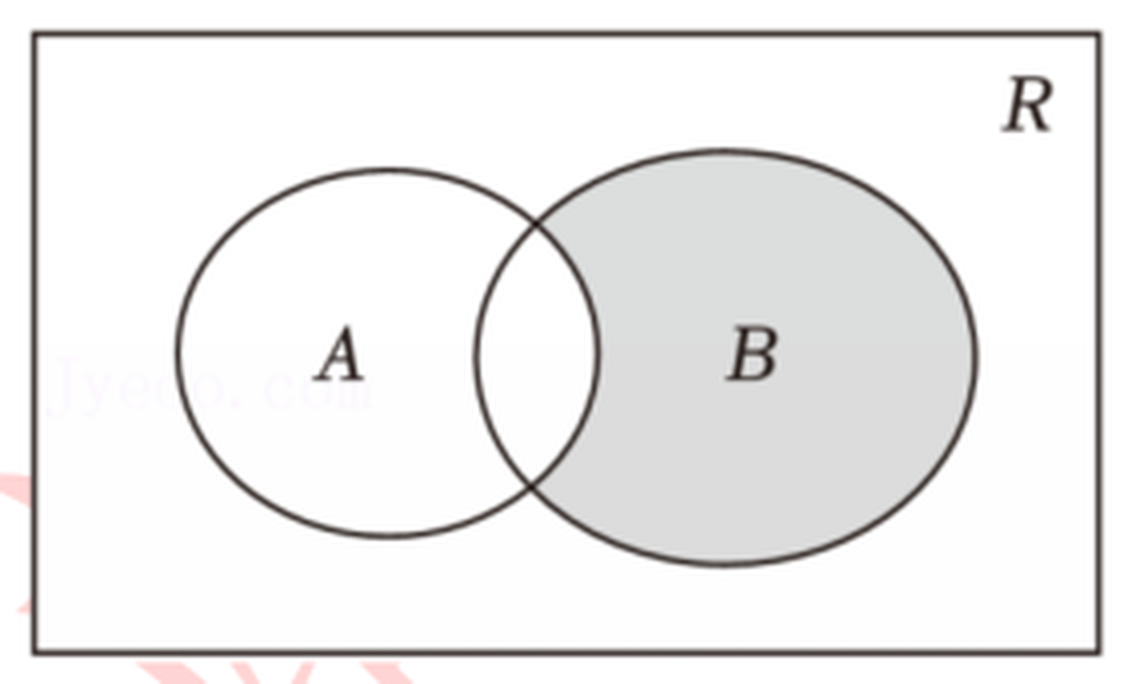
\includegraphics[width=0.30\textwidth]{figures/venn_Abar_cap_B.png}
\end{center}

\begin{enumerate}[label=(\arabic*)]
\item 若 $a=1$，求阴影部分表示的集合.
\item 若 $A\cap B=B$，求实数 $a$ 的取值范围.
\end{enumerate}

\ifanswer
\solbegin
\stepm{(1)}{因为 $\dfrac{2x-3}{x+5}\leqslant0$，
等价于 $\begin{cases}(2x-3)(x+5)\leqslant0\\ x+5\neq0\end{cases}$，}
\step{解得 $-5<x\leqslant\dfrac32$，即 $A=\left\{x\mid-5<x\leqslant\dfrac32\right\}$；}
\step{若 $a=1$，因为 $|x-1|<1$，等价于 $-1<x-1<1$，}
\step{解得 $0<x<2$，即 $B=\{x\mid0<x<2\}$.}
\step{由 Venn 图得阴影部分表示的集合为 $\overline{A}\cap B=\left(\dfrac32,2\right)$.}
\stepm{(2)}{由 (1) 得 $A=\left\{x\mid-5<x\leqslant\dfrac32\right\}$，}
\step{$B=\{x\mid|x-a|<1\}=\{x\mid-1+a<x<1+a\}\neq\varnothing$，}
\step{因为 $A\cap B=B$，所以 $B\sub A$，}
\step{所以 $\begin{cases}-5\leqslant-1+a\\ 1+a\leqslant\dfrac32\end{cases}$，
解得 $-4\leqslant a\leqslant\dfrac12$，}
\step{所以实数 $a$ 的取值范围为 $\left[-4,\dfrac12\right]$.}
\solend

\fi

\ansspace[6]

\item 设 $A=\{x\mid x^2-(m+3)x+2(m+1)=0,m\in\R\}$，
$B=\{x\mid 2x^2+(3n+1)x+2=0,n\in\R\}$.

\begin{enumerate}[label=(\arabic*)]
\item 是否存在 $m$、$n\in\R$，使得 $A=\{1,2\}$，$B=\varnothing$，说明理由；
\item 若 $A\cap B=A$，求 $m$、$n$ 的值.
\end{enumerate}

\ifanswer
\solbegin
\stepm{(1)}{由 $A=\{1,2\}$，得 $m=0$，}
\step{再由 $B=\varnothing$，得 $\Delta=(3n+1)^2-4\times2\times2=9n^2+6n-15<0$，}
\step{所以 $(3n+5)(n-1)<0$，解得 $-\dfrac53<n<1$，}
\step{故存在 $m=0$，$-\dfrac53<n<1$，使得 $A=\{1,2\}$，$B=\varnothing$.}
\stepm{(2)}{由 $x^2-(m+3)x+2(m+1)=0$，得 $x=2$ 或 $x=m+1$，}
\step{若 $A\cap B=A$，则 $A\sub B$，}
\step{将 $x=2$ 代入 $2x^2+(3n+1)x+2=0$，得 $n=-2$，}
\step{则 $B=\{x\mid 2x^2+(3n+1)x+2=0,n\in\R\}=\{x\mid 2x^2-5x+2=0\}
=\left\{2,\dfrac12\right\}$.}
\step{则 $m+1=\dfrac12$ 或 $m+1=2$，则 $m=-\dfrac12$ 或 $m=1$，
所以 $m=-\dfrac12$ 或 $m=1$，$n=-2$.}
\solend

\fi

\ansspace[6]

\item 已知陈述句 $\alpha$：关于 $x$ 的方程 $x^2-6x+m=0$ 有两个不同的正数根，陈述句
$\beta$：集合 $\{x\mid(m+1)x^2+4x+1=0,x\in\R\}$ 中至多有一个元素.

\begin{enumerate}[label=(\arabic*)]
\item 若 $\alpha$ 和 $\beta$ 都是真命题，求实数 $m$ 的取值范围；
\item 若 $\alpha$ 和 $\beta$ 至多有一个是假命题，求实数 $m$ 的取值范围.
\end{enumerate}

\ifanswer
\solbegin
\stepm{(1)}{因为关于 $x$ 的方程 $x^2-6x+m=0$ 有两个不同的正数根，}
\step{则 $\begin{cases}36-4m>0\\ m>0\end{cases}$，解得 $0<m<9$，}
\step{集合 $\{x\mid(m+1)x^2+4x+1=0,x\in\R\}$ 中至多有一个元素，}
\step{则 $m=-1$ 或 $\begin{cases}m+1\neq0\\ 16-4(m+1)\leqslant0\end{cases}$，
解得 $m\geqslant3$，}
\step{$\alpha$ 和 $\beta$ 都是真命题，所以实数 $m$ 的取值范围为 $\{m\mid3\leqslant m<9\}$}
\stepm{(2)}{由 (1) 得当 $\alpha$ 为假命题时，$m\leqslant0$ 或 $m\geqslant9$，}
\step{当 $\beta$ 为假命题时，$m<3$ 且 $m\neq-1$，}
\step{所以 $\alpha$ 和 $\beta$ 均为假命题时，$m$ 的范围是 $m\leqslant0$ 且 $m\neq-1$，}
\step{$\alpha$ 和 $\beta$ 至多有一个是假命题时，实数 $m$ 的取值范围为
$\{m\mid m>0$ 或 $m=-1\}$.}
\solend

\fi

\ansspace[6]

\item 已知符号 $[x]$ 表示不大于 $x$ 的最大整数 $(x\in\R)$，例如：$[1.3]=1$，
$[2]=2$，$[-1.2]=-2$.

\begin{enumerate}[label=(\arabic*)]
\item 已知方程 $[x]=3$，求该方程的解集；
\item 设方程 $\bigl[|x|+|x-1|\bigr]=3$ 的解集为 $A$，
集合 $B=\{x\mid 2x^2-11kx+15k^2\geqslant0\}$，若 $A\cup B=\R$，求实数 $k$ 的取值范围；
\item 在 (2) 的条件下，集合 $C=\{x\mid x^2-ax+1-2a\leqslant0,a\in\R\}$，是否存在实数
$a$，$A\cap C=A$，若存在，请求出实数 $a$ 的取值范围；若不存在，请说明理由.
\end{enumerate}

\ifanswer
\solbegin
\stepm{(1)}{方程 $[x]=3$，则 $x\in[3,4)$，所以该方程的解集为 $[3,4)$；}
\stepm{(2)}{因为 $\bigl[|x|+|x-1|\bigr]=3$，所以 $3\leqslant|x|+|x-1|<4$，}
\step{由绝对值不等式的几何意义得 $A=\left(-\dfrac32,-1\right]\cup\left[2,\dfrac52\right)$，}
\step{又 $B=\{x\mid 2x^2-11kx+15k^2\geqslant0\}=\{x\mid(2x-5k)(x-k)\geqslant0\}$，}
\step{当 $k=0$ 时，$B=\{x\mid 2x^2\geqslant0\}=\R$，则 $A\cup B=\R$，符合题意；}
\step{当 $k>0$ 时，$B=\left(-\infty,\dfrac{5k}{2}\right]\cup[3k,+\infty)$，
若 $A\cup B=\R$，}
\step{则 $\begin{cases}\dfrac{5k}{2}\geqslant2\\[2pt] 3k\leqslant\dfrac52\end{cases}$，
解得 $k\in\left[\dfrac45,\dfrac56\right]$；}
\step{当 $k<0$ 时，$B=(-\infty,3k]\cup\left[\dfrac{5k}{2},+\infty\right)$，
若 $A\cup B=\R$，}
\step{则 $\begin{cases}\dfrac{5k}{2}\leqslant-1\\[2pt] 3k\geqslant-\dfrac32\end{cases}$，
解得 $k\in\left[-\dfrac12,-\dfrac25\right]$.}
\step{综上所述，实数 $k$ 的取值范围为
$\left[-\dfrac12,-\dfrac25\right]\cup\{0\}\cup\left[\dfrac45,\dfrac56\right]$；}
\stepm{(3)}{因为 $A\cap C=A$，则 $A\sub C$ 且
$A=\left(-\dfrac32,-1\right]\cup\left[2,\dfrac52\right)$，}
\step{设集合 $C$ 的解集为 $(x_1,x_2)(x_1<x_2)$，}
\step{则 $\begin{cases}x_1\leqslant-\dfrac32\\[2pt] x_2\geqslant\dfrac52\end{cases}$，}
\step{所以
$\begin{cases}\Delta=a^2-4(1-2a)>0\\[2pt]
f\!\left(-\dfrac32\right)=\dfrac94+\dfrac32a+1-2a\leqslant0\\[4pt]
f\!\left(\dfrac52\right)=\dfrac{25}{4}-\dfrac52a+1-2a\leqslant0\end{cases}$，
解得 $a\geqslant\dfrac{13}{2}$，}
\step{故实数 $a$ 的取值范围为 $\left[\dfrac{13}{2},+\infty\right)$.}
\solend

\fi

\ansspace[6]

\item 非空有限集合 $S$ 是由若干个正实数组成，集合 $S$ 的元素个数不少于 $2$ 个. 对于任意
$a,b\in S,a\neq b$，若数 $a^b$ 或 $b^a$ 中至少有一个属于 $S$，则称集合 $S$ 是“好集”；
否则，称集合 $S$ 是“坏集”.

\begin{enumerate}[label=(\arabic*)]
\item 判断 $A=\{1,3,9\}$ 和 $B=\left\{1,\dfrac12,\dfrac14,\dfrac1{16}\right\}$ 是“好集”
还是“坏集”，并简单说明理由；
\item 题设的有限集 $S$ 中，既有大于 $1$ 的元素，又有小于 $1$ 的元素，证明：集合 $S$ 是
“坏集”；
\item 若题设中的 $a^b$ 或 $b^a$ 都属于 $S$，则称集合 $S$ 为“超级好集”，写出一个
“超级好集”（无须证明）.
\end{enumerate}

\ifanswer
\solbegin
\stepm{(1)}{$A=\{1,3,9\}$，$3^9\notin A$，$9^3\notin A$，所以 $A$ 是“坏集”，}
\step{从 $B$ 集合中任意取两个数字都满足需求，所以 $B$ 是“好集”.}
\stepm{(2)}{假设 $a$ 是 $S$ 中小于 $1$ 的元素中的最小元素，}
\step{$b$ 是 $S$ 中大于 $1$ 的元素中的最小元素，则 $a^b<a^1=a$，}
\step{所以 $a$ 就不是 $S$ 中小于 $1$ 的元素中的最小元素，即 $a^b\notin S$，}
\step{同理 $1=b^0<b^a<b^1=b$，所以 $b$ 就不是 $S$ 中大于 $1$ 的元素中的最小元素，}
\step{即 $b^a\notin S$，所以集合 $S$ 是“坏集”；}
\stepm{(3)}{首先 $S=\{1,a\}$（$a\neq1$ 且 $a>0$）是“超级好集”，}
\step{假设 $0<a<1$，由 (2) 得，$S$ 中不可能有大于 $1$ 的元素，}
\step{假设 $S$ 中有除 $a$ 之外的元素 $b\in S$（$a\neq b,b<1$），}
\step{假设 $a$ 是 $S$ 中小于 $1$ 的元素中的最大元素，$a^b>a^1=a$，}
\step{所以 $a$ 不是最大元素，所以 $a^b\notin S$，所以 $b\notin S$；}
\step{假设 $a>1$，由 (2) 得 $S$ 中不可能有小于 $1$ 的元素，}
\step{假设 $S$ 中有除 $a$ 之外的元素 $b$（$b>1$ 且 $b\neq a$），}
\step{假设 $a$ 是 $S$ 中大于 $1$ 的元素中的最小元素，则 $a^b>a^1=a$，}
\step{所以 $a$ 不是最小元素，即不存在 $b>1$，使得 $b\in S$，即 $b\notin S$，}
\step{综上，$S=\{1,a\}$（$a\neq1$ 且 $a>0$）.}
\solend

\fi

\ansspace*[10]

\end{enumerate}

\end{document}
"
% 紧凑版：xelatex "\def\iscompact{1}% 高一25_华师大二附中_周末作业3.tex
%   —— 高一上数学「2026-2027 年华师大二附中高一上周末作业 3」（试卷版/答案版）
% 试卷版：xelatex 高一25_华师大二附中_周末作业3.tex
% 答案版：xelatex "\def\isanswer{1}\input{高一25_华师大二附中_周末作业3.tex}"
% 紧凑版：xelatex "\def\iscompact{1}\input{高一25_华师大二附中_周末作业3.tex}"
%
% 原始材料是微信公众号图文（公众号「魔都数学加油站」连载「27学年高一 25」，2026-09-21 发布，
% 原文标题「27学年高一25——2026-2027年上海市华师大二附中高一上周末作业3」），
% 正文为 10 张 PNG 页（1080×1527，各页同尺寸）。原文本身就是一份**讲评版**——
% 题目下方直接印出【解析】（本卷无单独的【答案】行，填空题答案都写在解析里）。
% 试题文字与解析均照原卷录入，未改内容。卷面的粉色斜水印「魔都数学加油站」属水印，未录入。
%
% 卷首标题：原卷印作「2026-2027 年华师大二附中高一上周末作业 3」（公众号标题里的「上海市」
% 三字卷面标题行没有，本稿照卷面），年份区间按全稿惯例排 en dash，前缀照原卷保留「年」。
%
% 与原卷的排版差异（均已在 README「说明」中交代）：
%   ① 原文自**第 3 题**起（第 1、2 题未在该文中发布），故本稿题号亦自 3 起；
%   ② 原卷本就印有「一、填空题」「二、选择题」「三、解答题」三节标题，本稿照原卷分节，
%      只把标题改排成全稿统一的「大节标题」样式；
%   ③ 原卷第 13 题的答案「D」直接印在题干末尾的括号内，第 14—16 题的括号空着、答案写在
%      解析末句「故选 C／B」里；填空题的答案也都嵌在解析里，本稿统一改为试卷版隐去、
%      答案版以 \ans{} 给出（选择题另附【解析】），使两版彻底分离；
%   ④ 补集符号原卷一律作**上横线**（$\overline{A}$、$\overline{A\cup B}$），与同校的
%      高一14 同例，本稿照录（不改为 $\complement_U A$ 写法）；
%   ⑤ 原卷的实数集 R 斜体与粗体混用（第 17 题题干「全集为 R」作粗体，第 5、14 题与
%      第 16 题解析的 $R$ 为斜体），本稿按全稿惯例统一写作 $\R$；
%   ⑥ 原卷填空的横线约两个字宽，本稿按全稿惯例统一排 \blankline[4.4em]；
%   ⑦ 原卷未印副标题，本稿按全稿惯例补出副标题「集合与常用逻辑用语」；
%   ⑧ 第 17 题的 Venn 图原卷印在题干右侧（第 6 页），本稿移至题干之后；
%      图取原卷截图、4× LANCZOS 放大（figures/venn_Abar_cap_B.png，
%      阴影为 $B$ 中不含 $A\cap B$ 的部分，即 $\overline{A}\cap B$）。
%
% 原卷存疑两处（均照抄原卷、未改，见源码中该处上方注释）：
%   ① 第 8 题【解析】第二段「当 $\Delta=a^2-16>0$ 时，方程 $x^2+ax+4=0$ 有两个相同的根
%      $x_1$、$x_2$」——$\Delta>0$ 应为「两个**不**相同的根」（其自己的后文就把 $x_1$、$x_2$
%      当作可以不同的两个根在讨论），显系笔误；
%   ② 第 11 题【解析】先写「偶数必是 $2^{11}\cdot3^m\cdot337^n$，$m$、$n\in\N^*$」，
%      下一行又写「$0\leqslant m\leqslant10$，$0\leqslant n\leqslant10$，共有 121 种情况」
%      ——按 $\N^*$ 应从 1 起（至多 $10\times10=100$ 种），与 121（$=11\times11$，含 0）
%      对不上，两处至少有一处笔误。

\documentclass[a4paper,11pt]{article}
\usepackage{common}

\begin{document}

\examtitlest[3]{2026--2027 年华师大二附中高一上周末作业 3}{集合与常用逻辑用语}

\bigsec{一、填空题}

\begin{enumerate}
\setcounter{enumi}{2}

\item 设全集 $U=\{2,4,m^2+m-5\}$，集合 $A=\{2,1-m\}$，若 $\overline{A}=\{1\}$，则实数
$m=$ \blankline[4.4em].

\ifanswer
\solbegin
\step{因为 $\overline{A}=\{1\}$，所以 $1\in U$，$1\notin A$，}
\step{所以 $\begin{cases}m^2+m-5=1\\ 1-m\neq1\\ 1-m=4\end{cases}$，解得 $m=-3$.}
\solend

\fi

\item 已知条件 $\alpha$：$m<x\leqslant2m+5$，条件 $\beta$：$0\leqslant x\leqslant1$，
若 $\alpha$ 是 $\beta$ 的必要条件，则实数 $m$ 的取值范围为 \blankline[4.4em].

\ifanswer
\solbegin
\step{若 $\alpha$ 是 $\beta$ 的必要条件，则 $[0,1]\sub(m,2m+5]$，}
\step{所以 $\begin{cases}m<2m+5\\ m<0\\ 2m+5\geqslant1\end{cases}$，}
\step{解得 $-2\leqslant m<0$，故实数 $m$ 的取值范围为 $[-2,0)$.}
\solend

\fi

\item 已知 $\R$ 是全集，集合 $A=\{y\mid y=-x^2+1,x\in\R\}$，集合
$B=\{x\mid x=3+|a|,a\in\R\}$，则 $\overline{A\cup B}=$ \blankline[4.4em].

\ifanswer
\solbegin
\step{$A=\{y\mid y=-x^2+1,x\in\R\}=(-\infty,1]$，}
\step{$B=\{x\mid x=3+|a|,a\in\R\}=[3,+\infty)$，}
\step{所以 $\overline{A\cup B}=(1,3)$.}
\solend

\fi

\item 已知 $a$ 为常数，集合 $A=\{x\mid x^2+x-6=0\}$，集合 $B=\{x\mid ax-2=0\}$，且
$B\sub A$，则 $a$ 的所有取值构成的集合为 \blankline[4.4em].

\ifanswer
\solbegin
\step{集合 $A=\{-3,2\}$，因为 $B\sub A$，所以 $B=\varnothing$，$\{-3\}$，$\{2\}$，$\{-3,2\}$，}
\step{当 $B=\varnothing$ 时，$a=0$，当 $B=\{-3\}$ 时，$a=-\dfrac23$，当 $B=\{2\}$ 时，$a=1$，}
\step{当 $B=\{-3,2\}$ 时，不成立，故 $a$ 的取值集合为 $\left\{0,-\dfrac23,1\right\}$.}
\solend

\fi

\item 已知一元二次方程 $x^2+px+p=0$ 有两个不相等的实根分别为 $x_1$、$x_2$.
$A=x_1^2+x_2^2$，$B=x_1x_2(x_1+x_2)$，$A$ 与 $B$ 的大小为 \blankline[4.4em].

\ifanswer
\solbegin
\step{一元二次方程 $x^2+px+p=0$ 有两个不相等的实根分别为 $x_1$、$x_2$，}
\step{则 $\Delta=p^2-4p>0$，解得 $p<0$ 或 $p>4$，}
\step{由韦达定理得 $x_1+x_2=-p$，$x_1x_2=p$，}
\step{所以 $A=x_1^2+x_2^2=(x_1+x_2)^2-2x_1x_2=p^2-2p$，$B=x_1x_2(x_1+x_2)=-p^2$，}
\step{所以 $A-B=(p^2-2p)-(-p^2)=2p(p-1)$，}
\step{当 $p<0$ 时，则 $A-B>0$，故 $A>B$，}
\step{当 $p>4$ 时，则 $A-B>0$，故 $A>B$，}
\step{综上，$A=p^2-2p$，$B=-p^2$，且 $A>B$.}
\solend

\fi

\item 集合 $A=\{x\mid(x-1)(x^2+ax+4)=0,x\in\R\}$ 中所有元素之和为 $3$，则实数
$a=$ \blankline[4.4em].

\ifanswer
\solbegin
\step{当 $\Delta=a^2-16=0$ 时，方程 $x^2+ax+4=0$ 有两个相同的根 $-\dfrac a2$，}
\step{则 $A=\left\{1,-\dfrac a2\right\}$，故 $1-\dfrac a2=3$，解得 $a=-4$；}
% 注：下一行的「两个相同的根」系原卷笔误（△>0 应为「两个不相同的根」，其自己的后文
%     就把 x₁、x₂ 当作可以不同的两个根在讨论），照抄原卷、未改，见文件头「原卷存疑」①。
\step{当 $\Delta=a^2-16>0$ 时，方程 $x^2+ax+4=0$ 有两个相同的根 $x_1$、$x_2$，}
\step{若 $1$ 是方程 $x^2+ax+4=0$ 的根，则方程 $x^2+ax+4=0$ 的另一个根为 $4$，}
\step{则 $A=\{1,4\}$，不成立；}
\step{若 $1$ 不是方程 $x^2+ax+4=0$ 的根，则 $A=\{1,x_1,x_2\}$，则 $1+x_1+x_2=3$，}
\step{故 $x_1+x_2=2=-a$，故 $a=-2$（舍去）；}
\step{综上所述，$a=-4$.}
\solend

\fi

\item 已知集合 $A=\{x\mid x^2+2x-8\geqslant0\}$，$B=\{x\mid x^2-2ax+4\leqslant0\}$，
若 $a>0$，且 $A\cap B\cap\N$ 中恰有 $2$ 个元素，则 $a$ 的取值范围为 \blankline[4.4em].

\ifanswer
\solbegin
\step{由 $A$ 中不等式变形得 $(x-2)(x+4)\geqslant0$，解得 $x\leqslant-4$ 或 $x\geqslant2$，}
\step{即 $A=(-\infty,-4]\cup[2,+\infty)$，}
\step{设 $f(x)=x^2-2ax+4$，则 $f(x)$ 的轴对称 $x=a>0$，}
\step{且对应方程的根 $x_1$、$x_2$ 满足 $\begin{cases}x_1x_2=4\\ x_1+x_2>0\end{cases}$，}
\step{所以 $0<x_1\leqslant2\leqslant x_2$（取 $x_1\leqslant x_2$），}
\step{所以 $A\cap B\cap\N$ 中恰有的整数为 $2$，$3$，}
\step{所以 $\begin{cases}f(3)=9-6a+4\leqslant0\\ f(4)=16-8a+4>0\end{cases}$，}
\step{解得 $\dfrac{13}{6}\leqslant a<\dfrac52$，所以 $a$ 的取值范围为 $\left[\dfrac{13}{6},\dfrac52\right)$.}
\solend

\fi

\item 在三个关于 $x$ 的方程 $x^2-ax+4=0$，$x^2+(a-1)x+16=0$ 和
$x^2+2ax+3a+10=0$ 中至少有一个方程有实根，则实数 $a$ 的取值范围是 \blankline[4.4em].

\ifanswer
\solbegin
\step{当三个方程均无实根时，有}
\step{$\begin{cases}\Delta_1=a^2-16<0\\ \Delta_2=(a-1)^2-64<0\\ \Delta_3=4a^2-4(3a+10)<0\end{cases}$，}
\step{所以 $\begin{cases}-4<a<4\\ -7<a<9\\ -2<a<5\end{cases}$，}
\step{所以 $-2<a<4$，故三个方程均无实根时，$a$ 的取值范围为 $(-2,4)$，}
\step{所以三个方程中至少有一个方程有实根时，}
\step{实数 $a$ 的取值范围为 $(-\infty,-2]\cup[4,+\infty)$.}
\solend

\fi

% 注：下一行解析里的「m、n∈N*」与再下一行的「0≤m≤10，0≤n≤10，共有 121 种情况」
%     对不上（按 N* 应从 1 起，至多 10×10=100 种；121=11×11 含 0），系原卷自身矛盾，
%     照抄原卷、未改，见文件头「原卷存疑」②。
\item 若集合 $M=\{(x,y)\mid(x+1)+(x+2)+\cdots+(x+y)=2022^{10},x\in\Z,y\in\N^{*}\}$，
则集合 $M$ 中元素有 \blankline[4.4em] 个.

\ifanswer
\solbegin
\step{由题意得 $(x+1)+(x+2)+\cdots+(x+y)=\dfrac{y(2x+1+y)}{2}$，}
\step{所以 $y(2x+1+y)=2^{11}\cdot3^{10}\cdot337^{10}$，}
\step{因为 $y$ 与 $2x+1+y$ 必为一奇一偶，偶数必是 $2^{11}\cdot3^m\cdot337^n$，
$m$、$n\in\N^{*}$，}
\step{$0\leqslant m\leqslant10$，$0\leqslant n\leqslant10$，共有 $121$ 种情况，}
\step{因为 $y$ 与 $2x+1+y$ 奇偶未定，所以集合 $M$ 中元素只有 $242$ 个.}
\solend

\fi

\item 设集合 $M=\left\{x\mid m\leqslant x\leqslant m+\dfrac34\right\}$，
$N=\left\{x\mid n-\dfrac13\leqslant x\leqslant n\right\}$，且 $M$、$N$ 都是集合
$\{x\mid0\leqslant x\leqslant1\}$ 的子集，如果把 $b-a$ 叫做集合
$\{x\mid a\leqslant x\leqslant b\}$ 的长度，那么集合 $M\cap N$ 的长度的最小值是
\blankline[4.4em].

\ifanswer
\solbegin
\step{$M$ 的长度为 $\dfrac34$，$N$ 的长度为 $\dfrac13$，}
\step{当集合 $M\cap N$ 的长度的最小值时，$M$ 与 $N$ 应分别在区间 $[0,1]$ 的左右两端，}
\step{故 $M\cap N$ 的长度的最小值是 $\dfrac34+\dfrac13-1=\dfrac1{12}$.}
\solend

\fi

\end{enumerate}

\bigsec{二、选择题}

\begin{enumerate}
\setcounter{enumi}{12}

\item 直角坐标平面中除去两点 $A(1,1)$、$B(2,-2)$ 可用集合表示为\mbox{（\quad）}

\keepwithprev
A. $\{(x,y)\mid x\neq1,y\neq1,x\neq2,y\neq-2$\}\qquad
B. $\{(x,y)\mid\begin{cases}x\neq1\\ y\neq1\end{cases}$ 或 $\begin{cases}x\neq2\\ y\neq-2\end{cases}\}$

C. $\{(x,y)\mid[(x-1)^2+(y-1)^2][(x-2)^2+(y+2)^2]\neq0$\}

D. $\{(x,y)\mid[(x-1)^2+(y-1)^2]+[(x-2)^2+(y+2)^2]\neq0$\}

\ans{$D$}

\item 已知函数 $f(x)=x^2+nx$，记集合 $A=\{x\mid f(x)=0,x\in\R\}$，
$B=\{x\mid f(f(x))=0,x\in\R\}$，若 $A=B\neq\varnothing$，则 $n$ 的取值范围是\mbox{（\quad）}

\keepwithprev
A. $[0,4]$\qquad B. $(0,4)$\qquad C. $[0,4)$\qquad D. $(0,4]$

\ans{$C$}

\ifanswer
\solbegin
\step{$f(x)=x^2+nx$，$f[f(x)]=(x^2+nx)^2+n(x^2+nx)=(x^2+nx)(x^2+nx+n)$，}
\step{当 $n=0$ 时，$f(x)=x^2$，$f[f(x)]=x^4$，满足 $A=B$，此时 $n=0$；}
\step{当 $n\neq0$ 时，$0$、$-n$ 不是 $x^2+nx+n=0$ 的根，故 $\Delta=n^2-4n<0$，
解得 $0<n<4$，}
\step{综上所述，$n$ 的取值范围是 $[0,4)$. 故选 $C$.}
\solend

\fi

\item 设全集 $U=\{1,2,3,4,5,6,7,8,9,10\}$，给出条件：① $A\sub U$；②若 $x\in A$，
则 $2x\notin A$；③若 $x\in\overline{A}$，则 $2x\notin\overline{A}$.
那么同时满足三个条件的集合 $A$ 的个数为\mbox{（\quad）}

\keepwithprev
A. $0$ 个\qquad B. $16$ 个\qquad C. $32$ 个\qquad D. $64$ 个

\ans{$C$}

\ifanswer
\solbegin
\step{由① $A\sub U$；②若 $x\in A$，则 $2x\notin A$；③若 $x\in\overline{A}$，
则 $2x\notin\overline{A}$.}
\step{若 $1\in A$，则 $2\notin A$，即 $2\in\overline{A}$，则 $4\notin\overline{A}$，
即 $4\in A$，则 $8\notin A$，即 $8\in\overline{A}$；}
\step{若 $3\in A$，则 $6\notin A$，即 $6\in\overline{A}$；若 $5\in A$，则 $10\notin A$，
即 $10\in\overline{A}$，}
\step{故 $1$、$4$ 和 $2$、$8$ 分开，$3$ 和 $6$ 分开，$5$ 和 $10$ 分开，$7$ 和 $9$ 随意，}
\step{故同时满足三个条件的集合 $A$ 的个数为 $2\times2\times2\times2\times2=32$，
故选 $C$.}
\solend

\fi

\item 设集合 $P_1=\{x\mid x^2+ax+1>0\}$，$P_2=\{x\mid x^2+ax+2>0\}$，
$Q_1=\{x\mid x^2+x+b>0\}$，$Q_2=\{x\mid x^2+2x+b>0\}$，其中 $a$、$b\in\R$，
下列说法中正确的是\mbox{（\quad）}

\keepwithprev
A. 对任意 $a$，$P_1$ 是 $P_2$ 的子集，对任意的 $b$，$Q_1$ 不是 $Q_2$ 的子集

B. 对任意 $a$，$P_1$ 是 $P_2$ 的子集，存在 $b$，使得 $Q_1$ 是 $Q_2$ 的子集

C. 存在 $a$，使得 $P_1$ 不是 $P_2$ 的子集，对任意的 $b$，$Q_1$ 不是 $Q_2$ 的子集

D. 存在 $a$，使得 $P_1$ 不是 $P_2$ 的子集，存在 $b$，使得 $Q_1$ 是 $Q_2$ 的子集

\ans{$B$}

\ifanswer
\solbegin
\step{对于集合 $P_1=\{x\mid x^2+ax+1>0\}$，$P_2=\{x\mid x^2+ax+2>0\}$，}
\step{得当 $m\in P_1$ 时，即 $m^2+am+1>0$，得 $m^2+am+2>0$，}
\step{即有 $m\in P_2$，得对任意 $a$，$P_1$ 是 $P_2$ 的子集，}
\step{对于集合 $Q_1=\{x\mid x^2+x+b>0\}$，$Q_2=\{x\mid x^2+2x+b>0\}$，}
\step{当 $b=6$ 时，$Q_1=\{x\mid x^2+x+6>0\}=\R$，$Q_2=\{x\mid x^2+2x+6>0\}=\R$，}
\step{得 $Q_1$ 是 $Q_2$ 的子集，}
\step{当 $b=1$ 时，$Q_1=\{x\mid x^2+x+1>0\}=\R$，}
\step{$Q_2=\{x\mid x^2+2x+1>0\}=\{x\mid x\neq-1\}$，得 $Q_1$ 不是 $Q_2$ 的子集，}
\step{所以存在 $b$，使得 $Q_1$ 是 $Q_2$ 的子集，故选 $B$.}
\solend

\fi

\end{enumerate}

\bigsec{三、解答题}

\begin{enumerate}
\setcounter{enumi}{16}

\item 已知集合 $A=\left\{x\mid\dfrac{2x-3}{x+5}\leqslant0\right\}$，
$B=\{x\mid|x-a|<1\}$，全集为 $\R$.

\begin{center}
% 图取原卷截图、4× LANCZOS 放大（原卷把图印在题干右侧，本稿移至此处，见文件头⑧）。
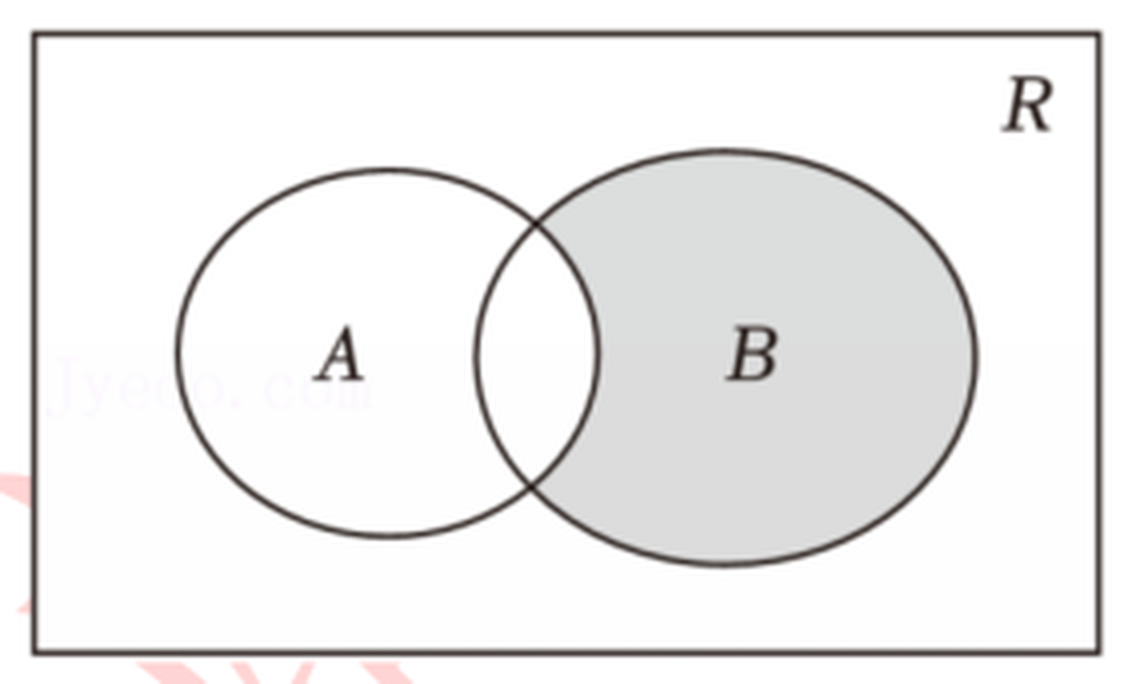
\includegraphics[width=0.30\textwidth]{figures/venn_Abar_cap_B.png}
\end{center}

\begin{enumerate}[label=(\arabic*)]
\item 若 $a=1$，求阴影部分表示的集合.
\item 若 $A\cap B=B$，求实数 $a$ 的取值范围.
\end{enumerate}

\ifanswer
\solbegin
\stepm{(1)}{因为 $\dfrac{2x-3}{x+5}\leqslant0$，
等价于 $\begin{cases}(2x-3)(x+5)\leqslant0\\ x+5\neq0\end{cases}$，}
\step{解得 $-5<x\leqslant\dfrac32$，即 $A=\left\{x\mid-5<x\leqslant\dfrac32\right\}$；}
\step{若 $a=1$，因为 $|x-1|<1$，等价于 $-1<x-1<1$，}
\step{解得 $0<x<2$，即 $B=\{x\mid0<x<2\}$.}
\step{由 Venn 图得阴影部分表示的集合为 $\overline{A}\cap B=\left(\dfrac32,2\right)$.}
\stepm{(2)}{由 (1) 得 $A=\left\{x\mid-5<x\leqslant\dfrac32\right\}$，}
\step{$B=\{x\mid|x-a|<1\}=\{x\mid-1+a<x<1+a\}\neq\varnothing$，}
\step{因为 $A\cap B=B$，所以 $B\sub A$，}
\step{所以 $\begin{cases}-5\leqslant-1+a\\ 1+a\leqslant\dfrac32\end{cases}$，
解得 $-4\leqslant a\leqslant\dfrac12$，}
\step{所以实数 $a$ 的取值范围为 $\left[-4,\dfrac12\right]$.}
\solend

\fi

\ansspace[6]

\item 设 $A=\{x\mid x^2-(m+3)x+2(m+1)=0,m\in\R\}$，
$B=\{x\mid 2x^2+(3n+1)x+2=0,n\in\R\}$.

\begin{enumerate}[label=(\arabic*)]
\item 是否存在 $m$、$n\in\R$，使得 $A=\{1,2\}$，$B=\varnothing$，说明理由；
\item 若 $A\cap B=A$，求 $m$、$n$ 的值.
\end{enumerate}

\ifanswer
\solbegin
\stepm{(1)}{由 $A=\{1,2\}$，得 $m=0$，}
\step{再由 $B=\varnothing$，得 $\Delta=(3n+1)^2-4\times2\times2=9n^2+6n-15<0$，}
\step{所以 $(3n+5)(n-1)<0$，解得 $-\dfrac53<n<1$，}
\step{故存在 $m=0$，$-\dfrac53<n<1$，使得 $A=\{1,2\}$，$B=\varnothing$.}
\stepm{(2)}{由 $x^2-(m+3)x+2(m+1)=0$，得 $x=2$ 或 $x=m+1$，}
\step{若 $A\cap B=A$，则 $A\sub B$，}
\step{将 $x=2$ 代入 $2x^2+(3n+1)x+2=0$，得 $n=-2$，}
\step{则 $B=\{x\mid 2x^2+(3n+1)x+2=0,n\in\R\}=\{x\mid 2x^2-5x+2=0\}
=\left\{2,\dfrac12\right\}$.}
\step{则 $m+1=\dfrac12$ 或 $m+1=2$，则 $m=-\dfrac12$ 或 $m=1$，
所以 $m=-\dfrac12$ 或 $m=1$，$n=-2$.}
\solend

\fi

\ansspace[6]

\item 已知陈述句 $\alpha$：关于 $x$ 的方程 $x^2-6x+m=0$ 有两个不同的正数根，陈述句
$\beta$：集合 $\{x\mid(m+1)x^2+4x+1=0,x\in\R\}$ 中至多有一个元素.

\begin{enumerate}[label=(\arabic*)]
\item 若 $\alpha$ 和 $\beta$ 都是真命题，求实数 $m$ 的取值范围；
\item 若 $\alpha$ 和 $\beta$ 至多有一个是假命题，求实数 $m$ 的取值范围.
\end{enumerate}

\ifanswer
\solbegin
\stepm{(1)}{因为关于 $x$ 的方程 $x^2-6x+m=0$ 有两个不同的正数根，}
\step{则 $\begin{cases}36-4m>0\\ m>0\end{cases}$，解得 $0<m<9$，}
\step{集合 $\{x\mid(m+1)x^2+4x+1=0,x\in\R\}$ 中至多有一个元素，}
\step{则 $m=-1$ 或 $\begin{cases}m+1\neq0\\ 16-4(m+1)\leqslant0\end{cases}$，
解得 $m\geqslant3$，}
\step{$\alpha$ 和 $\beta$ 都是真命题，所以实数 $m$ 的取值范围为 $\{m\mid3\leqslant m<9\}$}
\stepm{(2)}{由 (1) 得当 $\alpha$ 为假命题时，$m\leqslant0$ 或 $m\geqslant9$，}
\step{当 $\beta$ 为假命题时，$m<3$ 且 $m\neq-1$，}
\step{所以 $\alpha$ 和 $\beta$ 均为假命题时，$m$ 的范围是 $m\leqslant0$ 且 $m\neq-1$，}
\step{$\alpha$ 和 $\beta$ 至多有一个是假命题时，实数 $m$ 的取值范围为
$\{m\mid m>0$ 或 $m=-1\}$.}
\solend

\fi

\ansspace[6]

\item 已知符号 $[x]$ 表示不大于 $x$ 的最大整数 $(x\in\R)$，例如：$[1.3]=1$，
$[2]=2$，$[-1.2]=-2$.

\begin{enumerate}[label=(\arabic*)]
\item 已知方程 $[x]=3$，求该方程的解集；
\item 设方程 $\bigl[|x|+|x-1|\bigr]=3$ 的解集为 $A$，
集合 $B=\{x\mid 2x^2-11kx+15k^2\geqslant0\}$，若 $A\cup B=\R$，求实数 $k$ 的取值范围；
\item 在 (2) 的条件下，集合 $C=\{x\mid x^2-ax+1-2a\leqslant0,a\in\R\}$，是否存在实数
$a$，$A\cap C=A$，若存在，请求出实数 $a$ 的取值范围；若不存在，请说明理由.
\end{enumerate}

\ifanswer
\solbegin
\stepm{(1)}{方程 $[x]=3$，则 $x\in[3,4)$，所以该方程的解集为 $[3,4)$；}
\stepm{(2)}{因为 $\bigl[|x|+|x-1|\bigr]=3$，所以 $3\leqslant|x|+|x-1|<4$，}
\step{由绝对值不等式的几何意义得 $A=\left(-\dfrac32,-1\right]\cup\left[2,\dfrac52\right)$，}
\step{又 $B=\{x\mid 2x^2-11kx+15k^2\geqslant0\}=\{x\mid(2x-5k)(x-k)\geqslant0\}$，}
\step{当 $k=0$ 时，$B=\{x\mid 2x^2\geqslant0\}=\R$，则 $A\cup B=\R$，符合题意；}
\step{当 $k>0$ 时，$B=\left(-\infty,\dfrac{5k}{2}\right]\cup[3k,+\infty)$，
若 $A\cup B=\R$，}
\step{则 $\begin{cases}\dfrac{5k}{2}\geqslant2\\[2pt] 3k\leqslant\dfrac52\end{cases}$，
解得 $k\in\left[\dfrac45,\dfrac56\right]$；}
\step{当 $k<0$ 时，$B=(-\infty,3k]\cup\left[\dfrac{5k}{2},+\infty\right)$，
若 $A\cup B=\R$，}
\step{则 $\begin{cases}\dfrac{5k}{2}\leqslant-1\\[2pt] 3k\geqslant-\dfrac32\end{cases}$，
解得 $k\in\left[-\dfrac12,-\dfrac25\right]$.}
\step{综上所述，实数 $k$ 的取值范围为
$\left[-\dfrac12,-\dfrac25\right]\cup\{0\}\cup\left[\dfrac45,\dfrac56\right]$；}
\stepm{(3)}{因为 $A\cap C=A$，则 $A\sub C$ 且
$A=\left(-\dfrac32,-1\right]\cup\left[2,\dfrac52\right)$，}
\step{设集合 $C$ 的解集为 $(x_1,x_2)(x_1<x_2)$，}
\step{则 $\begin{cases}x_1\leqslant-\dfrac32\\[2pt] x_2\geqslant\dfrac52\end{cases}$，}
\step{所以
$\begin{cases}\Delta=a^2-4(1-2a)>0\\[2pt]
f\!\left(-\dfrac32\right)=\dfrac94+\dfrac32a+1-2a\leqslant0\\[4pt]
f\!\left(\dfrac52\right)=\dfrac{25}{4}-\dfrac52a+1-2a\leqslant0\end{cases}$，
解得 $a\geqslant\dfrac{13}{2}$，}
\step{故实数 $a$ 的取值范围为 $\left[\dfrac{13}{2},+\infty\right)$.}
\solend

\fi

\ansspace[6]

\item 非空有限集合 $S$ 是由若干个正实数组成，集合 $S$ 的元素个数不少于 $2$ 个. 对于任意
$a,b\in S,a\neq b$，若数 $a^b$ 或 $b^a$ 中至少有一个属于 $S$，则称集合 $S$ 是“好集”；
否则，称集合 $S$ 是“坏集”.

\begin{enumerate}[label=(\arabic*)]
\item 判断 $A=\{1,3,9\}$ 和 $B=\left\{1,\dfrac12,\dfrac14,\dfrac1{16}\right\}$ 是“好集”
还是“坏集”，并简单说明理由；
\item 题设的有限集 $S$ 中，既有大于 $1$ 的元素，又有小于 $1$ 的元素，证明：集合 $S$ 是
“坏集”；
\item 若题设中的 $a^b$ 或 $b^a$ 都属于 $S$，则称集合 $S$ 为“超级好集”，写出一个
“超级好集”（无须证明）.
\end{enumerate}

\ifanswer
\solbegin
\stepm{(1)}{$A=\{1,3,9\}$，$3^9\notin A$，$9^3\notin A$，所以 $A$ 是“坏集”，}
\step{从 $B$ 集合中任意取两个数字都满足需求，所以 $B$ 是“好集”.}
\stepm{(2)}{假设 $a$ 是 $S$ 中小于 $1$ 的元素中的最小元素，}
\step{$b$ 是 $S$ 中大于 $1$ 的元素中的最小元素，则 $a^b<a^1=a$，}
\step{所以 $a$ 就不是 $S$ 中小于 $1$ 的元素中的最小元素，即 $a^b\notin S$，}
\step{同理 $1=b^0<b^a<b^1=b$，所以 $b$ 就不是 $S$ 中大于 $1$ 的元素中的最小元素，}
\step{即 $b^a\notin S$，所以集合 $S$ 是“坏集”；}
\stepm{(3)}{首先 $S=\{1,a\}$（$a\neq1$ 且 $a>0$）是“超级好集”，}
\step{假设 $0<a<1$，由 (2) 得，$S$ 中不可能有大于 $1$ 的元素，}
\step{假设 $S$ 中有除 $a$ 之外的元素 $b\in S$（$a\neq b,b<1$），}
\step{假设 $a$ 是 $S$ 中小于 $1$ 的元素中的最大元素，$a^b>a^1=a$，}
\step{所以 $a$ 不是最大元素，所以 $a^b\notin S$，所以 $b\notin S$；}
\step{假设 $a>1$，由 (2) 得 $S$ 中不可能有小于 $1$ 的元素，}
\step{假设 $S$ 中有除 $a$ 之外的元素 $b$（$b>1$ 且 $b\neq a$），}
\step{假设 $a$ 是 $S$ 中大于 $1$ 的元素中的最小元素，则 $a^b>a^1=a$，}
\step{所以 $a$ 不是最小元素，即不存在 $b>1$，使得 $b\in S$，即 $b\notin S$，}
\step{综上，$S=\{1,a\}$（$a\neq1$ 且 $a>0$）.}
\solend

\fi

\ansspace*[10]

\end{enumerate}

\end{document}
"
%
% 原始材料是微信公众号图文（公众号「魔都数学加油站」连载「27学年高一 25」，2026-09-21 发布，
% 原文标题「27学年高一25——2026-2027年上海市华师大二附中高一上周末作业3」），
% 正文为 10 张 PNG 页（1080×1527，各页同尺寸）。原文本身就是一份**讲评版**——
% 题目下方直接印出【解析】（本卷无单独的【答案】行，填空题答案都写在解析里）。
% 试题文字与解析均照原卷录入，未改内容。卷面的粉色斜水印「魔都数学加油站」属水印，未录入。
%
% 卷首标题：原卷印作「2026-2027 年华师大二附中高一上周末作业 3」（公众号标题里的「上海市」
% 三字卷面标题行没有，本稿照卷面），年份区间按全稿惯例排 en dash，前缀照原卷保留「年」。
%
% 与原卷的排版差异（均已在 README「说明」中交代）：
%   ① 原文自**第 3 题**起（第 1、2 题未在该文中发布），故本稿题号亦自 3 起；
%   ② 原卷本就印有「一、填空题」「二、选择题」「三、解答题」三节标题，本稿照原卷分节，
%      只把标题改排成全稿统一的「大节标题」样式；
%   ③ 原卷第 13 题的答案「D」直接印在题干末尾的括号内，第 14—16 题的括号空着、答案写在
%      解析末句「故选 C／B」里；填空题的答案也都嵌在解析里，本稿统一改为试卷版隐去、
%      答案版以 \ans{} 给出（选择题另附【解析】），使两版彻底分离；
%   ④ 补集符号原卷一律作**上横线**（$\overline{A}$、$\overline{A\cup B}$），与同校的
%      高一14 同例，本稿照录（不改为 $\complement_U A$ 写法）；
%   ⑤ 原卷的实数集 R 斜体与粗体混用（第 17 题题干「全集为 R」作粗体，第 5、14 题与
%      第 16 题解析的 $R$ 为斜体），本稿按全稿惯例统一写作 $\R$；
%   ⑥ 原卷填空的横线约两个字宽，本稿按全稿惯例统一排 \blankline[4.4em]；
%   ⑦ 原卷未印副标题，本稿按全稿惯例补出副标题「集合与常用逻辑用语」；
%   ⑧ 第 17 题的 Venn 图原卷印在题干右侧（第 6 页），本稿移至题干之后；
%      图取原卷截图、4× LANCZOS 放大（figures/venn_Abar_cap_B.png，
%      阴影为 $B$ 中不含 $A\cap B$ 的部分，即 $\overline{A}\cap B$）。
%
% 原卷存疑两处（均照抄原卷、未改，见源码中该处上方注释）：
%   ① 第 8 题【解析】第二段「当 $\Delta=a^2-16>0$ 时，方程 $x^2+ax+4=0$ 有两个相同的根
%      $x_1$、$x_2$」——$\Delta>0$ 应为「两个**不**相同的根」（其自己的后文就把 $x_1$、$x_2$
%      当作可以不同的两个根在讨论），显系笔误；
%   ② 第 11 题【解析】先写「偶数必是 $2^{11}\cdot3^m\cdot337^n$，$m$、$n\in\N^*$」，
%      下一行又写「$0\leqslant m\leqslant10$，$0\leqslant n\leqslant10$，共有 121 种情况」
%      ——按 $\N^*$ 应从 1 起（至多 $10\times10=100$ 种），与 121（$=11\times11$，含 0）
%      对不上，两处至少有一处笔误。

\documentclass[a4paper,11pt]{article}
\usepackage{common}

\begin{document}

\examtitlest[3]{2026--2027 年华师大二附中高一上周末作业 3}{集合与常用逻辑用语}

\bigsec{一、填空题}

\begin{enumerate}
\setcounter{enumi}{2}

\item 设全集 $U=\{2,4,m^2+m-5\}$，集合 $A=\{2,1-m\}$，若 $\overline{A}=\{1\}$，则实数
$m=$ \blankline[4.4em].

\ifanswer
\solbegin
\step{因为 $\overline{A}=\{1\}$，所以 $1\in U$，$1\notin A$，}
\step{所以 $\begin{cases}m^2+m-5=1\\ 1-m\neq1\\ 1-m=4\end{cases}$，解得 $m=-3$.}
\solend

\fi

\item 已知条件 $\alpha$：$m<x\leqslant2m+5$，条件 $\beta$：$0\leqslant x\leqslant1$，
若 $\alpha$ 是 $\beta$ 的必要条件，则实数 $m$ 的取值范围为 \blankline[4.4em].

\ifanswer
\solbegin
\step{若 $\alpha$ 是 $\beta$ 的必要条件，则 $[0,1]\sub(m,2m+5]$，}
\step{所以 $\begin{cases}m<2m+5\\ m<0\\ 2m+5\geqslant1\end{cases}$，}
\step{解得 $-2\leqslant m<0$，故实数 $m$ 的取值范围为 $[-2,0)$.}
\solend

\fi

\item 已知 $\R$ 是全集，集合 $A=\{y\mid y=-x^2+1,x\in\R\}$，集合
$B=\{x\mid x=3+|a|,a\in\R\}$，则 $\overline{A\cup B}=$ \blankline[4.4em].

\ifanswer
\solbegin
\step{$A=\{y\mid y=-x^2+1,x\in\R\}=(-\infty,1]$，}
\step{$B=\{x\mid x=3+|a|,a\in\R\}=[3,+\infty)$，}
\step{所以 $\overline{A\cup B}=(1,3)$.}
\solend

\fi

\item 已知 $a$ 为常数，集合 $A=\{x\mid x^2+x-6=0\}$，集合 $B=\{x\mid ax-2=0\}$，且
$B\sub A$，则 $a$ 的所有取值构成的集合为 \blankline[4.4em].

\ifanswer
\solbegin
\step{集合 $A=\{-3,2\}$，因为 $B\sub A$，所以 $B=\varnothing$，$\{-3\}$，$\{2\}$，$\{-3,2\}$，}
\step{当 $B=\varnothing$ 时，$a=0$，当 $B=\{-3\}$ 时，$a=-\dfrac23$，当 $B=\{2\}$ 时，$a=1$，}
\step{当 $B=\{-3,2\}$ 时，不成立，故 $a$ 的取值集合为 $\left\{0,-\dfrac23,1\right\}$.}
\solend

\fi

\item 已知一元二次方程 $x^2+px+p=0$ 有两个不相等的实根分别为 $x_1$、$x_2$.
$A=x_1^2+x_2^2$，$B=x_1x_2(x_1+x_2)$，$A$ 与 $B$ 的大小为 \blankline[4.4em].

\ifanswer
\solbegin
\step{一元二次方程 $x^2+px+p=0$ 有两个不相等的实根分别为 $x_1$、$x_2$，}
\step{则 $\Delta=p^2-4p>0$，解得 $p<0$ 或 $p>4$，}
\step{由韦达定理得 $x_1+x_2=-p$，$x_1x_2=p$，}
\step{所以 $A=x_1^2+x_2^2=(x_1+x_2)^2-2x_1x_2=p^2-2p$，$B=x_1x_2(x_1+x_2)=-p^2$，}
\step{所以 $A-B=(p^2-2p)-(-p^2)=2p(p-1)$，}
\step{当 $p<0$ 时，则 $A-B>0$，故 $A>B$，}
\step{当 $p>4$ 时，则 $A-B>0$，故 $A>B$，}
\step{综上，$A=p^2-2p$，$B=-p^2$，且 $A>B$.}
\solend

\fi

\item 集合 $A=\{x\mid(x-1)(x^2+ax+4)=0,x\in\R\}$ 中所有元素之和为 $3$，则实数
$a=$ \blankline[4.4em].

\ifanswer
\solbegin
\step{当 $\Delta=a^2-16=0$ 时，方程 $x^2+ax+4=0$ 有两个相同的根 $-\dfrac a2$，}
\step{则 $A=\left\{1,-\dfrac a2\right\}$，故 $1-\dfrac a2=3$，解得 $a=-4$；}
% 注：下一行的「两个相同的根」系原卷笔误（△>0 应为「两个不相同的根」，其自己的后文
%     就把 x₁、x₂ 当作可以不同的两个根在讨论），照抄原卷、未改，见文件头「原卷存疑」①。
\step{当 $\Delta=a^2-16>0$ 时，方程 $x^2+ax+4=0$ 有两个相同的根 $x_1$、$x_2$，}
\step{若 $1$ 是方程 $x^2+ax+4=0$ 的根，则方程 $x^2+ax+4=0$ 的另一个根为 $4$，}
\step{则 $A=\{1,4\}$，不成立；}
\step{若 $1$ 不是方程 $x^2+ax+4=0$ 的根，则 $A=\{1,x_1,x_2\}$，则 $1+x_1+x_2=3$，}
\step{故 $x_1+x_2=2=-a$，故 $a=-2$（舍去）；}
\step{综上所述，$a=-4$.}
\solend

\fi

\item 已知集合 $A=\{x\mid x^2+2x-8\geqslant0\}$，$B=\{x\mid x^2-2ax+4\leqslant0\}$，
若 $a>0$，且 $A\cap B\cap\N$ 中恰有 $2$ 个元素，则 $a$ 的取值范围为 \blankline[4.4em].

\ifanswer
\solbegin
\step{由 $A$ 中不等式变形得 $(x-2)(x+4)\geqslant0$，解得 $x\leqslant-4$ 或 $x\geqslant2$，}
\step{即 $A=(-\infty,-4]\cup[2,+\infty)$，}
\step{设 $f(x)=x^2-2ax+4$，则 $f(x)$ 的轴对称 $x=a>0$，}
\step{且对应方程的根 $x_1$、$x_2$ 满足 $\begin{cases}x_1x_2=4\\ x_1+x_2>0\end{cases}$，}
\step{所以 $0<x_1\leqslant2\leqslant x_2$（取 $x_1\leqslant x_2$），}
\step{所以 $A\cap B\cap\N$ 中恰有的整数为 $2$，$3$，}
\step{所以 $\begin{cases}f(3)=9-6a+4\leqslant0\\ f(4)=16-8a+4>0\end{cases}$，}
\step{解得 $\dfrac{13}{6}\leqslant a<\dfrac52$，所以 $a$ 的取值范围为 $\left[\dfrac{13}{6},\dfrac52\right)$.}
\solend

\fi

\item 在三个关于 $x$ 的方程 $x^2-ax+4=0$，$x^2+(a-1)x+16=0$ 和
$x^2+2ax+3a+10=0$ 中至少有一个方程有实根，则实数 $a$ 的取值范围是 \blankline[4.4em].

\ifanswer
\solbegin
\step{当三个方程均无实根时，有}
\step{$\begin{cases}\Delta_1=a^2-16<0\\ \Delta_2=(a-1)^2-64<0\\ \Delta_3=4a^2-4(3a+10)<0\end{cases}$，}
\step{所以 $\begin{cases}-4<a<4\\ -7<a<9\\ -2<a<5\end{cases}$，}
\step{所以 $-2<a<4$，故三个方程均无实根时，$a$ 的取值范围为 $(-2,4)$，}
\step{所以三个方程中至少有一个方程有实根时，}
\step{实数 $a$ 的取值范围为 $(-\infty,-2]\cup[4,+\infty)$.}
\solend

\fi

% 注：下一行解析里的「m、n∈N*」与再下一行的「0≤m≤10，0≤n≤10，共有 121 种情况」
%     对不上（按 N* 应从 1 起，至多 10×10=100 种；121=11×11 含 0），系原卷自身矛盾，
%     照抄原卷、未改，见文件头「原卷存疑」②。
\item 若集合 $M=\{(x,y)\mid(x+1)+(x+2)+\cdots+(x+y)=2022^{10},x\in\Z,y\in\N^{*}\}$，
则集合 $M$ 中元素有 \blankline[4.4em] 个.

\ifanswer
\solbegin
\step{由题意得 $(x+1)+(x+2)+\cdots+(x+y)=\dfrac{y(2x+1+y)}{2}$，}
\step{所以 $y(2x+1+y)=2^{11}\cdot3^{10}\cdot337^{10}$，}
\step{因为 $y$ 与 $2x+1+y$ 必为一奇一偶，偶数必是 $2^{11}\cdot3^m\cdot337^n$，
$m$、$n\in\N^{*}$，}
\step{$0\leqslant m\leqslant10$，$0\leqslant n\leqslant10$，共有 $121$ 种情况，}
\step{因为 $y$ 与 $2x+1+y$ 奇偶未定，所以集合 $M$ 中元素只有 $242$ 个.}
\solend

\fi

\item 设集合 $M=\left\{x\mid m\leqslant x\leqslant m+\dfrac34\right\}$，
$N=\left\{x\mid n-\dfrac13\leqslant x\leqslant n\right\}$，且 $M$、$N$ 都是集合
$\{x\mid0\leqslant x\leqslant1\}$ 的子集，如果把 $b-a$ 叫做集合
$\{x\mid a\leqslant x\leqslant b\}$ 的长度，那么集合 $M\cap N$ 的长度的最小值是
\blankline[4.4em].

\ifanswer
\solbegin
\step{$M$ 的长度为 $\dfrac34$，$N$ 的长度为 $\dfrac13$，}
\step{当集合 $M\cap N$ 的长度的最小值时，$M$ 与 $N$ 应分别在区间 $[0,1]$ 的左右两端，}
\step{故 $M\cap N$ 的长度的最小值是 $\dfrac34+\dfrac13-1=\dfrac1{12}$.}
\solend

\fi

\end{enumerate}

\bigsec{二、选择题}

\begin{enumerate}
\setcounter{enumi}{12}

\item 直角坐标平面中除去两点 $A(1,1)$、$B(2,-2)$ 可用集合表示为\mbox{（\quad）}

\keepwithprev
A. $\{(x,y)\mid x\neq1,y\neq1,x\neq2,y\neq-2$\}\qquad
B. $\{(x,y)\mid\begin{cases}x\neq1\\ y\neq1\end{cases}$ 或 $\begin{cases}x\neq2\\ y\neq-2\end{cases}\}$

C. $\{(x,y)\mid[(x-1)^2+(y-1)^2][(x-2)^2+(y+2)^2]\neq0$\}

D. $\{(x,y)\mid[(x-1)^2+(y-1)^2]+[(x-2)^2+(y+2)^2]\neq0$\}

\ans{$D$}

\item 已知函数 $f(x)=x^2+nx$，记集合 $A=\{x\mid f(x)=0,x\in\R\}$，
$B=\{x\mid f(f(x))=0,x\in\R\}$，若 $A=B\neq\varnothing$，则 $n$ 的取值范围是\mbox{（\quad）}

\keepwithprev
A. $[0,4]$\qquad B. $(0,4)$\qquad C. $[0,4)$\qquad D. $(0,4]$

\ans{$C$}

\ifanswer
\solbegin
\step{$f(x)=x^2+nx$，$f[f(x)]=(x^2+nx)^2+n(x^2+nx)=(x^2+nx)(x^2+nx+n)$，}
\step{当 $n=0$ 时，$f(x)=x^2$，$f[f(x)]=x^4$，满足 $A=B$，此时 $n=0$；}
\step{当 $n\neq0$ 时，$0$、$-n$ 不是 $x^2+nx+n=0$ 的根，故 $\Delta=n^2-4n<0$，
解得 $0<n<4$，}
\step{综上所述，$n$ 的取值范围是 $[0,4)$. 故选 $C$.}
\solend

\fi

\item 设全集 $U=\{1,2,3,4,5,6,7,8,9,10\}$，给出条件：① $A\sub U$；②若 $x\in A$，
则 $2x\notin A$；③若 $x\in\overline{A}$，则 $2x\notin\overline{A}$.
那么同时满足三个条件的集合 $A$ 的个数为\mbox{（\quad）}

\keepwithprev
A. $0$ 个\qquad B. $16$ 个\qquad C. $32$ 个\qquad D. $64$ 个

\ans{$C$}

\ifanswer
\solbegin
\step{由① $A\sub U$；②若 $x\in A$，则 $2x\notin A$；③若 $x\in\overline{A}$，
则 $2x\notin\overline{A}$.}
\step{若 $1\in A$，则 $2\notin A$，即 $2\in\overline{A}$，则 $4\notin\overline{A}$，
即 $4\in A$，则 $8\notin A$，即 $8\in\overline{A}$；}
\step{若 $3\in A$，则 $6\notin A$，即 $6\in\overline{A}$；若 $5\in A$，则 $10\notin A$，
即 $10\in\overline{A}$，}
\step{故 $1$、$4$ 和 $2$、$8$ 分开，$3$ 和 $6$ 分开，$5$ 和 $10$ 分开，$7$ 和 $9$ 随意，}
\step{故同时满足三个条件的集合 $A$ 的个数为 $2\times2\times2\times2\times2=32$，
故选 $C$.}
\solend

\fi

\item 设集合 $P_1=\{x\mid x^2+ax+1>0\}$，$P_2=\{x\mid x^2+ax+2>0\}$，
$Q_1=\{x\mid x^2+x+b>0\}$，$Q_2=\{x\mid x^2+2x+b>0\}$，其中 $a$、$b\in\R$，
下列说法中正确的是\mbox{（\quad）}

\keepwithprev
A. 对任意 $a$，$P_1$ 是 $P_2$ 的子集，对任意的 $b$，$Q_1$ 不是 $Q_2$ 的子集

B. 对任意 $a$，$P_1$ 是 $P_2$ 的子集，存在 $b$，使得 $Q_1$ 是 $Q_2$ 的子集

C. 存在 $a$，使得 $P_1$ 不是 $P_2$ 的子集，对任意的 $b$，$Q_1$ 不是 $Q_2$ 的子集

D. 存在 $a$，使得 $P_1$ 不是 $P_2$ 的子集，存在 $b$，使得 $Q_1$ 是 $Q_2$ 的子集

\ans{$B$}

\ifanswer
\solbegin
\step{对于集合 $P_1=\{x\mid x^2+ax+1>0\}$，$P_2=\{x\mid x^2+ax+2>0\}$，}
\step{得当 $m\in P_1$ 时，即 $m^2+am+1>0$，得 $m^2+am+2>0$，}
\step{即有 $m\in P_2$，得对任意 $a$，$P_1$ 是 $P_2$ 的子集，}
\step{对于集合 $Q_1=\{x\mid x^2+x+b>0\}$，$Q_2=\{x\mid x^2+2x+b>0\}$，}
\step{当 $b=6$ 时，$Q_1=\{x\mid x^2+x+6>0\}=\R$，$Q_2=\{x\mid x^2+2x+6>0\}=\R$，}
\step{得 $Q_1$ 是 $Q_2$ 的子集，}
\step{当 $b=1$ 时，$Q_1=\{x\mid x^2+x+1>0\}=\R$，}
\step{$Q_2=\{x\mid x^2+2x+1>0\}=\{x\mid x\neq-1\}$，得 $Q_1$ 不是 $Q_2$ 的子集，}
\step{所以存在 $b$，使得 $Q_1$ 是 $Q_2$ 的子集，故选 $B$.}
\solend

\fi

\end{enumerate}

\bigsec{三、解答题}

\begin{enumerate}
\setcounter{enumi}{16}

\item 已知集合 $A=\left\{x\mid\dfrac{2x-3}{x+5}\leqslant0\right\}$，
$B=\{x\mid|x-a|<1\}$，全集为 $\R$.

\begin{center}
% 图取原卷截图、4× LANCZOS 放大（原卷把图印在题干右侧，本稿移至此处，见文件头⑧）。
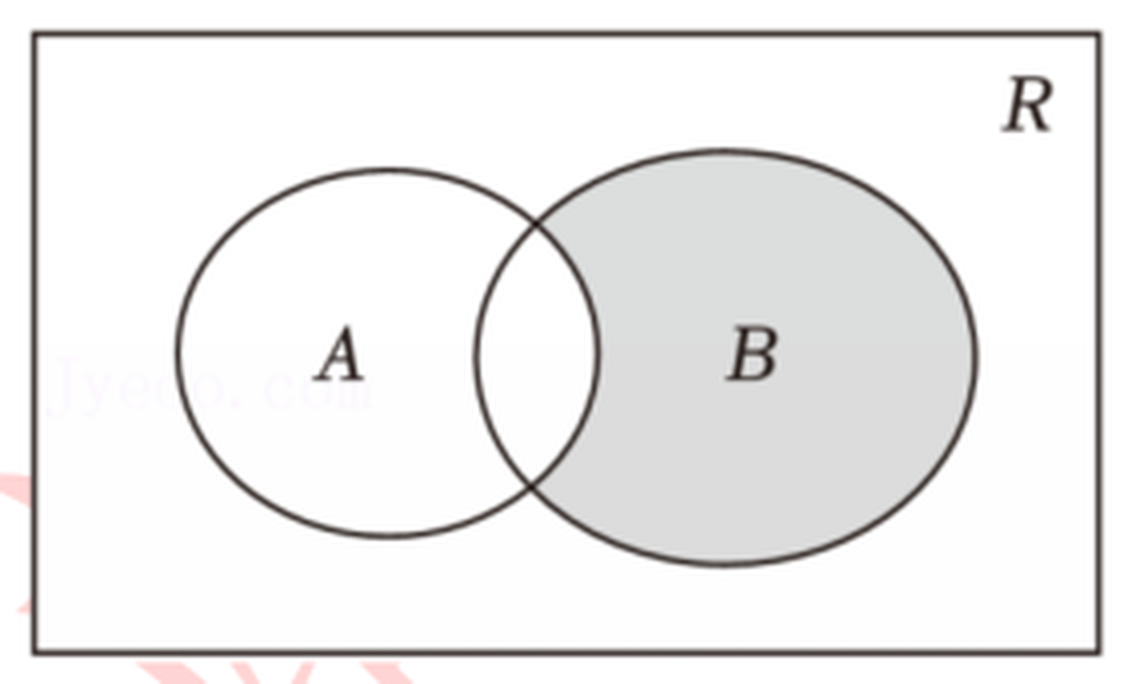
\includegraphics[width=0.30\textwidth]{figures/venn_Abar_cap_B.png}
\end{center}

\begin{enumerate}[label=(\arabic*)]
\item 若 $a=1$，求阴影部分表示的集合.
\item 若 $A\cap B=B$，求实数 $a$ 的取值范围.
\end{enumerate}

\ifanswer
\solbegin
\stepm{(1)}{因为 $\dfrac{2x-3}{x+5}\leqslant0$，
等价于 $\begin{cases}(2x-3)(x+5)\leqslant0\\ x+5\neq0\end{cases}$，}
\step{解得 $-5<x\leqslant\dfrac32$，即 $A=\left\{x\mid-5<x\leqslant\dfrac32\right\}$；}
\step{若 $a=1$，因为 $|x-1|<1$，等价于 $-1<x-1<1$，}
\step{解得 $0<x<2$，即 $B=\{x\mid0<x<2\}$.}
\step{由 Venn 图得阴影部分表示的集合为 $\overline{A}\cap B=\left(\dfrac32,2\right)$.}
\stepm{(2)}{由 (1) 得 $A=\left\{x\mid-5<x\leqslant\dfrac32\right\}$，}
\step{$B=\{x\mid|x-a|<1\}=\{x\mid-1+a<x<1+a\}\neq\varnothing$，}
\step{因为 $A\cap B=B$，所以 $B\sub A$，}
\step{所以 $\begin{cases}-5\leqslant-1+a\\ 1+a\leqslant\dfrac32\end{cases}$，
解得 $-4\leqslant a\leqslant\dfrac12$，}
\step{所以实数 $a$ 的取值范围为 $\left[-4,\dfrac12\right]$.}
\solend

\fi

\ansspace[6]

\item 设 $A=\{x\mid x^2-(m+3)x+2(m+1)=0,m\in\R\}$，
$B=\{x\mid 2x^2+(3n+1)x+2=0,n\in\R\}$.

\begin{enumerate}[label=(\arabic*)]
\item 是否存在 $m$、$n\in\R$，使得 $A=\{1,2\}$，$B=\varnothing$，说明理由；
\item 若 $A\cap B=A$，求 $m$、$n$ 的值.
\end{enumerate}

\ifanswer
\solbegin
\stepm{(1)}{由 $A=\{1,2\}$，得 $m=0$，}
\step{再由 $B=\varnothing$，得 $\Delta=(3n+1)^2-4\times2\times2=9n^2+6n-15<0$，}
\step{所以 $(3n+5)(n-1)<0$，解得 $-\dfrac53<n<1$，}
\step{故存在 $m=0$，$-\dfrac53<n<1$，使得 $A=\{1,2\}$，$B=\varnothing$.}
\stepm{(2)}{由 $x^2-(m+3)x+2(m+1)=0$，得 $x=2$ 或 $x=m+1$，}
\step{若 $A\cap B=A$，则 $A\sub B$，}
\step{将 $x=2$ 代入 $2x^2+(3n+1)x+2=0$，得 $n=-2$，}
\step{则 $B=\{x\mid 2x^2+(3n+1)x+2=0,n\in\R\}=\{x\mid 2x^2-5x+2=0\}
=\left\{2,\dfrac12\right\}$.}
\step{则 $m+1=\dfrac12$ 或 $m+1=2$，则 $m=-\dfrac12$ 或 $m=1$，
所以 $m=-\dfrac12$ 或 $m=1$，$n=-2$.}
\solend

\fi

\ansspace[6]

\item 已知陈述句 $\alpha$：关于 $x$ 的方程 $x^2-6x+m=0$ 有两个不同的正数根，陈述句
$\beta$：集合 $\{x\mid(m+1)x^2+4x+1=0,x\in\R\}$ 中至多有一个元素.

\begin{enumerate}[label=(\arabic*)]
\item 若 $\alpha$ 和 $\beta$ 都是真命题，求实数 $m$ 的取值范围；
\item 若 $\alpha$ 和 $\beta$ 至多有一个是假命题，求实数 $m$ 的取值范围.
\end{enumerate}

\ifanswer
\solbegin
\stepm{(1)}{因为关于 $x$ 的方程 $x^2-6x+m=0$ 有两个不同的正数根，}
\step{则 $\begin{cases}36-4m>0\\ m>0\end{cases}$，解得 $0<m<9$，}
\step{集合 $\{x\mid(m+1)x^2+4x+1=0,x\in\R\}$ 中至多有一个元素，}
\step{则 $m=-1$ 或 $\begin{cases}m+1\neq0\\ 16-4(m+1)\leqslant0\end{cases}$，
解得 $m\geqslant3$，}
\step{$\alpha$ 和 $\beta$ 都是真命题，所以实数 $m$ 的取值范围为 $\{m\mid3\leqslant m<9\}$}
\stepm{(2)}{由 (1) 得当 $\alpha$ 为假命题时，$m\leqslant0$ 或 $m\geqslant9$，}
\step{当 $\beta$ 为假命题时，$m<3$ 且 $m\neq-1$，}
\step{所以 $\alpha$ 和 $\beta$ 均为假命题时，$m$ 的范围是 $m\leqslant0$ 且 $m\neq-1$，}
\step{$\alpha$ 和 $\beta$ 至多有一个是假命题时，实数 $m$ 的取值范围为
$\{m\mid m>0$ 或 $m=-1\}$.}
\solend

\fi

\ansspace[6]

\item 已知符号 $[x]$ 表示不大于 $x$ 的最大整数 $(x\in\R)$，例如：$[1.3]=1$，
$[2]=2$，$[-1.2]=-2$.

\begin{enumerate}[label=(\arabic*)]
\item 已知方程 $[x]=3$，求该方程的解集；
\item 设方程 $\bigl[|x|+|x-1|\bigr]=3$ 的解集为 $A$，
集合 $B=\{x\mid 2x^2-11kx+15k^2\geqslant0\}$，若 $A\cup B=\R$，求实数 $k$ 的取值范围；
\item 在 (2) 的条件下，集合 $C=\{x\mid x^2-ax+1-2a\leqslant0,a\in\R\}$，是否存在实数
$a$，$A\cap C=A$，若存在，请求出实数 $a$ 的取值范围；若不存在，请说明理由.
\end{enumerate}

\ifanswer
\solbegin
\stepm{(1)}{方程 $[x]=3$，则 $x\in[3,4)$，所以该方程的解集为 $[3,4)$；}
\stepm{(2)}{因为 $\bigl[|x|+|x-1|\bigr]=3$，所以 $3\leqslant|x|+|x-1|<4$，}
\step{由绝对值不等式的几何意义得 $A=\left(-\dfrac32,-1\right]\cup\left[2,\dfrac52\right)$，}
\step{又 $B=\{x\mid 2x^2-11kx+15k^2\geqslant0\}=\{x\mid(2x-5k)(x-k)\geqslant0\}$，}
\step{当 $k=0$ 时，$B=\{x\mid 2x^2\geqslant0\}=\R$，则 $A\cup B=\R$，符合题意；}
\step{当 $k>0$ 时，$B=\left(-\infty,\dfrac{5k}{2}\right]\cup[3k,+\infty)$，
若 $A\cup B=\R$，}
\step{则 $\begin{cases}\dfrac{5k}{2}\geqslant2\\[2pt] 3k\leqslant\dfrac52\end{cases}$，
解得 $k\in\left[\dfrac45,\dfrac56\right]$；}
\step{当 $k<0$ 时，$B=(-\infty,3k]\cup\left[\dfrac{5k}{2},+\infty\right)$，
若 $A\cup B=\R$，}
\step{则 $\begin{cases}\dfrac{5k}{2}\leqslant-1\\[2pt] 3k\geqslant-\dfrac32\end{cases}$，
解得 $k\in\left[-\dfrac12,-\dfrac25\right]$.}
\step{综上所述，实数 $k$ 的取值范围为
$\left[-\dfrac12,-\dfrac25\right]\cup\{0\}\cup\left[\dfrac45,\dfrac56\right]$；}
\stepm{(3)}{因为 $A\cap C=A$，则 $A\sub C$ 且
$A=\left(-\dfrac32,-1\right]\cup\left[2,\dfrac52\right)$，}
\step{设集合 $C$ 的解集为 $(x_1,x_2)(x_1<x_2)$，}
\step{则 $\begin{cases}x_1\leqslant-\dfrac32\\[2pt] x_2\geqslant\dfrac52\end{cases}$，}
\step{所以
$\begin{cases}\Delta=a^2-4(1-2a)>0\\[2pt]
f\!\left(-\dfrac32\right)=\dfrac94+\dfrac32a+1-2a\leqslant0\\[4pt]
f\!\left(\dfrac52\right)=\dfrac{25}{4}-\dfrac52a+1-2a\leqslant0\end{cases}$，
解得 $a\geqslant\dfrac{13}{2}$，}
\step{故实数 $a$ 的取值范围为 $\left[\dfrac{13}{2},+\infty\right)$.}
\solend

\fi

\ansspace[6]

\item 非空有限集合 $S$ 是由若干个正实数组成，集合 $S$ 的元素个数不少于 $2$ 个. 对于任意
$a,b\in S,a\neq b$，若数 $a^b$ 或 $b^a$ 中至少有一个属于 $S$，则称集合 $S$ 是“好集”；
否则，称集合 $S$ 是“坏集”.

\begin{enumerate}[label=(\arabic*)]
\item 判断 $A=\{1,3,9\}$ 和 $B=\left\{1,\dfrac12,\dfrac14,\dfrac1{16}\right\}$ 是“好集”
还是“坏集”，并简单说明理由；
\item 题设的有限集 $S$ 中，既有大于 $1$ 的元素，又有小于 $1$ 的元素，证明：集合 $S$ 是
“坏集”；
\item 若题设中的 $a^b$ 或 $b^a$ 都属于 $S$，则称集合 $S$ 为“超级好集”，写出一个
“超级好集”（无须证明）.
\end{enumerate}

\ifanswer
\solbegin
\stepm{(1)}{$A=\{1,3,9\}$，$3^9\notin A$，$9^3\notin A$，所以 $A$ 是“坏集”，}
\step{从 $B$ 集合中任意取两个数字都满足需求，所以 $B$ 是“好集”.}
\stepm{(2)}{假设 $a$ 是 $S$ 中小于 $1$ 的元素中的最小元素，}
\step{$b$ 是 $S$ 中大于 $1$ 的元素中的最小元素，则 $a^b<a^1=a$，}
\step{所以 $a$ 就不是 $S$ 中小于 $1$ 的元素中的最小元素，即 $a^b\notin S$，}
\step{同理 $1=b^0<b^a<b^1=b$，所以 $b$ 就不是 $S$ 中大于 $1$ 的元素中的最小元素，}
\step{即 $b^a\notin S$，所以集合 $S$ 是“坏集”；}
\stepm{(3)}{首先 $S=\{1,a\}$（$a\neq1$ 且 $a>0$）是“超级好集”，}
\step{假设 $0<a<1$，由 (2) 得，$S$ 中不可能有大于 $1$ 的元素，}
\step{假设 $S$ 中有除 $a$ 之外的元素 $b\in S$（$a\neq b,b<1$），}
\step{假设 $a$ 是 $S$ 中小于 $1$ 的元素中的最大元素，$a^b>a^1=a$，}
\step{所以 $a$ 不是最大元素，所以 $a^b\notin S$，所以 $b\notin S$；}
\step{假设 $a>1$，由 (2) 得 $S$ 中不可能有小于 $1$ 的元素，}
\step{假设 $S$ 中有除 $a$ 之外的元素 $b$（$b>1$ 且 $b\neq a$），}
\step{假设 $a$ 是 $S$ 中大于 $1$ 的元素中的最小元素，则 $a^b>a^1=a$，}
\step{所以 $a$ 不是最小元素，即不存在 $b>1$，使得 $b\in S$，即 $b\notin S$，}
\step{综上，$S=\{1,a\}$（$a\neq1$ 且 $a>0$）.}
\solend

\fi

\ansspace*[10]

\end{enumerate}

\end{document}
"
%
% 原始材料是微信公众号图文（公众号「魔都数学加油站」连载「27学年高一 25」，2026-09-21 发布，
% 原文标题「27学年高一25——2026-2027年上海市华师大二附中高一上周末作业3」），
% 正文为 10 张 PNG 页（1080×1527，各页同尺寸）。原文本身就是一份**讲评版**——
% 题目下方直接印出【解析】（本卷无单独的【答案】行，填空题答案都写在解析里）。
% 试题文字与解析均照原卷录入，未改内容。卷面的粉色斜水印「魔都数学加油站」属水印，未录入。
%
% 卷首标题：原卷印作「2026-2027 年华师大二附中高一上周末作业 3」（公众号标题里的「上海市」
% 三字卷面标题行没有，本稿照卷面），年份区间按全稿惯例排 en dash，前缀照原卷保留「年」。
%
% 与原卷的排版差异（均已在 README「说明」中交代）：
%   ① 原文自**第 3 题**起（第 1、2 题未在该文中发布），故本稿题号亦自 3 起；
%   ② 原卷本就印有「一、填空题」「二、选择题」「三、解答题」三节标题，本稿照原卷分节，
%      只把标题改排成全稿统一的「大节标题」样式；
%   ③ 原卷第 13 题的答案「D」直接印在题干末尾的括号内，第 14—16 题的括号空着、答案写在
%      解析末句「故选 C／B」里；填空题的答案也都嵌在解析里，本稿统一改为试卷版隐去、
%      答案版以 \ans{} 给出（选择题另附【解析】），使两版彻底分离；
%   ④ 补集符号原卷一律作**上横线**（$\overline{A}$、$\overline{A\cup B}$），与同校的
%      高一14 同例，本稿照录（不改为 $\complement_U A$ 写法）；
%   ⑤ 原卷的实数集 R 斜体与粗体混用（第 17 题题干「全集为 R」作粗体，第 5、14 题与
%      第 16 题解析的 $R$ 为斜体），本稿按全稿惯例统一写作 $\R$；
%   ⑥ 原卷填空的横线约两个字宽，本稿按全稿惯例统一排 \blankline[4.4em]；
%   ⑦ 原卷未印副标题，本稿按全稿惯例补出副标题「集合与常用逻辑用语」；
%   ⑧ 第 17 题的 Venn 图原卷印在题干右侧（第 6 页），本稿移至题干之后；
%      图取原卷截图、4× LANCZOS 放大（figures/venn_Abar_cap_B.png，
%      阴影为 $B$ 中不含 $A\cap B$ 的部分，即 $\overline{A}\cap B$）。
%
% 原卷存疑两处（均照抄原卷、未改，见源码中该处上方注释）：
%   ① 第 8 题【解析】第二段「当 $\Delta=a^2-16>0$ 时，方程 $x^2+ax+4=0$ 有两个相同的根
%      $x_1$、$x_2$」——$\Delta>0$ 应为「两个**不**相同的根」（其自己的后文就把 $x_1$、$x_2$
%      当作可以不同的两个根在讨论），显系笔误；
%   ② 第 11 题【解析】先写「偶数必是 $2^{11}\cdot3^m\cdot337^n$，$m$、$n\in\N^*$」，
%      下一行又写「$0\leqslant m\leqslant10$，$0\leqslant n\leqslant10$，共有 121 种情况」
%      ——按 $\N^*$ 应从 1 起（至多 $10\times10=100$ 种），与 121（$=11\times11$，含 0）
%      对不上，两处至少有一处笔误。

\documentclass[a4paper,11pt]{article}
\usepackage{common}

\begin{document}

\examtitlest[3]{2026--2027 年华师大二附中高一上周末作业 3}{集合与常用逻辑用语}

\bigsec{一、填空题}

\begin{enumerate}
\setcounter{enumi}{2}

\item 设全集 $U=\{2,4,m^2+m-5\}$，集合 $A=\{2,1-m\}$，若 $\overline{A}=\{1\}$，则实数
$m=$ \blankline[4.4em].

\ifanswer
\solbegin
\step{因为 $\overline{A}=\{1\}$，所以 $1\in U$，$1\notin A$，}
\step{所以 $\begin{cases}m^2+m-5=1\\ 1-m\neq1\\ 1-m=4\end{cases}$，解得 $m=-3$.}
\solend

\fi

\item 已知条件 $\alpha$：$m<x\leqslant2m+5$，条件 $\beta$：$0\leqslant x\leqslant1$，
若 $\alpha$ 是 $\beta$ 的必要条件，则实数 $m$ 的取值范围为 \blankline[4.4em].

\ifanswer
\solbegin
\step{若 $\alpha$ 是 $\beta$ 的必要条件，则 $[0,1]\sub(m,2m+5]$，}
\step{所以 $\begin{cases}m<2m+5\\ m<0\\ 2m+5\geqslant1\end{cases}$，}
\step{解得 $-2\leqslant m<0$，故实数 $m$ 的取值范围为 $[-2,0)$.}
\solend

\fi

\item 已知 $\R$ 是全集，集合 $A=\{y\mid y=-x^2+1,x\in\R\}$，集合
$B=\{x\mid x=3+|a|,a\in\R\}$，则 $\overline{A\cup B}=$ \blankline[4.4em].

\ifanswer
\solbegin
\step{$A=\{y\mid y=-x^2+1,x\in\R\}=(-\infty,1]$，}
\step{$B=\{x\mid x=3+|a|,a\in\R\}=[3,+\infty)$，}
\step{所以 $\overline{A\cup B}=(1,3)$.}
\solend

\fi

\item 已知 $a$ 为常数，集合 $A=\{x\mid x^2+x-6=0\}$，集合 $B=\{x\mid ax-2=0\}$，且
$B\sub A$，则 $a$ 的所有取值构成的集合为 \blankline[4.4em].

\ifanswer
\solbegin
\step{集合 $A=\{-3,2\}$，因为 $B\sub A$，所以 $B=\varnothing$，$\{-3\}$，$\{2\}$，$\{-3,2\}$，}
\step{当 $B=\varnothing$ 时，$a=0$，当 $B=\{-3\}$ 时，$a=-\dfrac23$，当 $B=\{2\}$ 时，$a=1$，}
\step{当 $B=\{-3,2\}$ 时，不成立，故 $a$ 的取值集合为 $\left\{0,-\dfrac23,1\right\}$.}
\solend

\fi

\item 已知一元二次方程 $x^2+px+p=0$ 有两个不相等的实根分别为 $x_1$、$x_2$.
$A=x_1^2+x_2^2$，$B=x_1x_2(x_1+x_2)$，$A$ 与 $B$ 的大小为 \blankline[4.4em].

\ifanswer
\solbegin
\step{一元二次方程 $x^2+px+p=0$ 有两个不相等的实根分别为 $x_1$、$x_2$，}
\step{则 $\Delta=p^2-4p>0$，解得 $p<0$ 或 $p>4$，}
\step{由韦达定理得 $x_1+x_2=-p$，$x_1x_2=p$，}
\step{所以 $A=x_1^2+x_2^2=(x_1+x_2)^2-2x_1x_2=p^2-2p$，$B=x_1x_2(x_1+x_2)=-p^2$，}
\step{所以 $A-B=(p^2-2p)-(-p^2)=2p(p-1)$，}
\step{当 $p<0$ 时，则 $A-B>0$，故 $A>B$，}
\step{当 $p>4$ 时，则 $A-B>0$，故 $A>B$，}
\step{综上，$A=p^2-2p$，$B=-p^2$，且 $A>B$.}
\solend

\fi

\item 集合 $A=\{x\mid(x-1)(x^2+ax+4)=0,x\in\R\}$ 中所有元素之和为 $3$，则实数
$a=$ \blankline[4.4em].

\ifanswer
\solbegin
\step{当 $\Delta=a^2-16=0$ 时，方程 $x^2+ax+4=0$ 有两个相同的根 $-\dfrac a2$，}
\step{则 $A=\left\{1,-\dfrac a2\right\}$，故 $1-\dfrac a2=3$，解得 $a=-4$；}
% 注：下一行的「两个相同的根」系原卷笔误（△>0 应为「两个不相同的根」，其自己的后文
%     就把 x₁、x₂ 当作可以不同的两个根在讨论），照抄原卷、未改，见文件头「原卷存疑」①。
\step{当 $\Delta=a^2-16>0$ 时，方程 $x^2+ax+4=0$ 有两个相同的根 $x_1$、$x_2$，}
\step{若 $1$ 是方程 $x^2+ax+4=0$ 的根，则方程 $x^2+ax+4=0$ 的另一个根为 $4$，}
\step{则 $A=\{1,4\}$，不成立；}
\step{若 $1$ 不是方程 $x^2+ax+4=0$ 的根，则 $A=\{1,x_1,x_2\}$，则 $1+x_1+x_2=3$，}
\step{故 $x_1+x_2=2=-a$，故 $a=-2$（舍去）；}
\step{综上所述，$a=-4$.}
\solend

\fi

\item 已知集合 $A=\{x\mid x^2+2x-8\geqslant0\}$，$B=\{x\mid x^2-2ax+4\leqslant0\}$，
若 $a>0$，且 $A\cap B\cap\N$ 中恰有 $2$ 个元素，则 $a$ 的取值范围为 \blankline[4.4em].

\ifanswer
\solbegin
\step{由 $A$ 中不等式变形得 $(x-2)(x+4)\geqslant0$，解得 $x\leqslant-4$ 或 $x\geqslant2$，}
\step{即 $A=(-\infty,-4]\cup[2,+\infty)$，}
\step{设 $f(x)=x^2-2ax+4$，则 $f(x)$ 的轴对称 $x=a>0$，}
\step{且对应方程的根 $x_1$、$x_2$ 满足 $\begin{cases}x_1x_2=4\\ x_1+x_2>0\end{cases}$，}
\step{所以 $0<x_1\leqslant2\leqslant x_2$（取 $x_1\leqslant x_2$），}
\step{所以 $A\cap B\cap\N$ 中恰有的整数为 $2$，$3$，}
\step{所以 $\begin{cases}f(3)=9-6a+4\leqslant0\\ f(4)=16-8a+4>0\end{cases}$，}
\step{解得 $\dfrac{13}{6}\leqslant a<\dfrac52$，所以 $a$ 的取值范围为 $\left[\dfrac{13}{6},\dfrac52\right)$.}
\solend

\fi

\item 在三个关于 $x$ 的方程 $x^2-ax+4=0$，$x^2+(a-1)x+16=0$ 和
$x^2+2ax+3a+10=0$ 中至少有一个方程有实根，则实数 $a$ 的取值范围是 \blankline[4.4em].

\ifanswer
\solbegin
\step{当三个方程均无实根时，有}
\step{$\begin{cases}\Delta_1=a^2-16<0\\ \Delta_2=(a-1)^2-64<0\\ \Delta_3=4a^2-4(3a+10)<0\end{cases}$，}
\step{所以 $\begin{cases}-4<a<4\\ -7<a<9\\ -2<a<5\end{cases}$，}
\step{所以 $-2<a<4$，故三个方程均无实根时，$a$ 的取值范围为 $(-2,4)$，}
\step{所以三个方程中至少有一个方程有实根时，}
\step{实数 $a$ 的取值范围为 $(-\infty,-2]\cup[4,+\infty)$.}
\solend

\fi

% 注：下一行解析里的「m、n∈N*」与再下一行的「0≤m≤10，0≤n≤10，共有 121 种情况」
%     对不上（按 N* 应从 1 起，至多 10×10=100 种；121=11×11 含 0），系原卷自身矛盾，
%     照抄原卷、未改，见文件头「原卷存疑」②。
\item 若集合 $M=\{(x,y)\mid(x+1)+(x+2)+\cdots+(x+y)=2022^{10},x\in\Z,y\in\N^{*}\}$，
则集合 $M$ 中元素有 \blankline[4.4em] 个.

\ifanswer
\solbegin
\step{由题意得 $(x+1)+(x+2)+\cdots+(x+y)=\dfrac{y(2x+1+y)}{2}$，}
\step{所以 $y(2x+1+y)=2^{11}\cdot3^{10}\cdot337^{10}$，}
\step{因为 $y$ 与 $2x+1+y$ 必为一奇一偶，偶数必是 $2^{11}\cdot3^m\cdot337^n$，
$m$、$n\in\N^{*}$，}
\step{$0\leqslant m\leqslant10$，$0\leqslant n\leqslant10$，共有 $121$ 种情况，}
\step{因为 $y$ 与 $2x+1+y$ 奇偶未定，所以集合 $M$ 中元素只有 $242$ 个.}
\solend

\fi

\item 设集合 $M=\left\{x\mid m\leqslant x\leqslant m+\dfrac34\right\}$，
$N=\left\{x\mid n-\dfrac13\leqslant x\leqslant n\right\}$，且 $M$、$N$ 都是集合
$\{x\mid0\leqslant x\leqslant1\}$ 的子集，如果把 $b-a$ 叫做集合
$\{x\mid a\leqslant x\leqslant b\}$ 的长度，那么集合 $M\cap N$ 的长度的最小值是
\blankline[4.4em].

\ifanswer
\solbegin
\step{$M$ 的长度为 $\dfrac34$，$N$ 的长度为 $\dfrac13$，}
\step{当集合 $M\cap N$ 的长度的最小值时，$M$ 与 $N$ 应分别在区间 $[0,1]$ 的左右两端，}
\step{故 $M\cap N$ 的长度的最小值是 $\dfrac34+\dfrac13-1=\dfrac1{12}$.}
\solend

\fi

\end{enumerate}

\bigsec{二、选择题}

\begin{enumerate}
\setcounter{enumi}{12}

\item 直角坐标平面中除去两点 $A(1,1)$、$B(2,-2)$ 可用集合表示为\mbox{（\quad）}

\keepwithprev
A. $\{(x,y)\mid x\neq1,y\neq1,x\neq2,y\neq-2$\}\qquad
B. $\{(x,y)\mid\begin{cases}x\neq1\\ y\neq1\end{cases}$ 或 $\begin{cases}x\neq2\\ y\neq-2\end{cases}\}$

C. $\{(x,y)\mid[(x-1)^2+(y-1)^2][(x-2)^2+(y+2)^2]\neq0$\}

D. $\{(x,y)\mid[(x-1)^2+(y-1)^2]+[(x-2)^2+(y+2)^2]\neq0$\}

\ans{$D$}

\item 已知函数 $f(x)=x^2+nx$，记集合 $A=\{x\mid f(x)=0,x\in\R\}$，
$B=\{x\mid f(f(x))=0,x\in\R\}$，若 $A=B\neq\varnothing$，则 $n$ 的取值范围是\mbox{（\quad）}

\keepwithprev
A. $[0,4]$\qquad B. $(0,4)$\qquad C. $[0,4)$\qquad D. $(0,4]$

\ans{$C$}

\ifanswer
\solbegin
\step{$f(x)=x^2+nx$，$f[f(x)]=(x^2+nx)^2+n(x^2+nx)=(x^2+nx)(x^2+nx+n)$，}
\step{当 $n=0$ 时，$f(x)=x^2$，$f[f(x)]=x^4$，满足 $A=B$，此时 $n=0$；}
\step{当 $n\neq0$ 时，$0$、$-n$ 不是 $x^2+nx+n=0$ 的根，故 $\Delta=n^2-4n<0$，
解得 $0<n<4$，}
\step{综上所述，$n$ 的取值范围是 $[0,4)$. 故选 $C$.}
\solend

\fi

\item 设全集 $U=\{1,2,3,4,5,6,7,8,9,10\}$，给出条件：① $A\sub U$；②若 $x\in A$，
则 $2x\notin A$；③若 $x\in\overline{A}$，则 $2x\notin\overline{A}$.
那么同时满足三个条件的集合 $A$ 的个数为\mbox{（\quad）}

\keepwithprev
A. $0$ 个\qquad B. $16$ 个\qquad C. $32$ 个\qquad D. $64$ 个

\ans{$C$}

\ifanswer
\solbegin
\step{由① $A\sub U$；②若 $x\in A$，则 $2x\notin A$；③若 $x\in\overline{A}$，
则 $2x\notin\overline{A}$.}
\step{若 $1\in A$，则 $2\notin A$，即 $2\in\overline{A}$，则 $4\notin\overline{A}$，
即 $4\in A$，则 $8\notin A$，即 $8\in\overline{A}$；}
\step{若 $3\in A$，则 $6\notin A$，即 $6\in\overline{A}$；若 $5\in A$，则 $10\notin A$，
即 $10\in\overline{A}$，}
\step{故 $1$、$4$ 和 $2$、$8$ 分开，$3$ 和 $6$ 分开，$5$ 和 $10$ 分开，$7$ 和 $9$ 随意，}
\step{故同时满足三个条件的集合 $A$ 的个数为 $2\times2\times2\times2\times2=32$，
故选 $C$.}
\solend

\fi

\item 设集合 $P_1=\{x\mid x^2+ax+1>0\}$，$P_2=\{x\mid x^2+ax+2>0\}$，
$Q_1=\{x\mid x^2+x+b>0\}$，$Q_2=\{x\mid x^2+2x+b>0\}$，其中 $a$、$b\in\R$，
下列说法中正确的是\mbox{（\quad）}

\keepwithprev
A. 对任意 $a$，$P_1$ 是 $P_2$ 的子集，对任意的 $b$，$Q_1$ 不是 $Q_2$ 的子集

B. 对任意 $a$，$P_1$ 是 $P_2$ 的子集，存在 $b$，使得 $Q_1$ 是 $Q_2$ 的子集

C. 存在 $a$，使得 $P_1$ 不是 $P_2$ 的子集，对任意的 $b$，$Q_1$ 不是 $Q_2$ 的子集

D. 存在 $a$，使得 $P_1$ 不是 $P_2$ 的子集，存在 $b$，使得 $Q_1$ 是 $Q_2$ 的子集

\ans{$B$}

\ifanswer
\solbegin
\step{对于集合 $P_1=\{x\mid x^2+ax+1>0\}$，$P_2=\{x\mid x^2+ax+2>0\}$，}
\step{得当 $m\in P_1$ 时，即 $m^2+am+1>0$，得 $m^2+am+2>0$，}
\step{即有 $m\in P_2$，得对任意 $a$，$P_1$ 是 $P_2$ 的子集，}
\step{对于集合 $Q_1=\{x\mid x^2+x+b>0\}$，$Q_2=\{x\mid x^2+2x+b>0\}$，}
\step{当 $b=6$ 时，$Q_1=\{x\mid x^2+x+6>0\}=\R$，$Q_2=\{x\mid x^2+2x+6>0\}=\R$，}
\step{得 $Q_1$ 是 $Q_2$ 的子集，}
\step{当 $b=1$ 时，$Q_1=\{x\mid x^2+x+1>0\}=\R$，}
\step{$Q_2=\{x\mid x^2+2x+1>0\}=\{x\mid x\neq-1\}$，得 $Q_1$ 不是 $Q_2$ 的子集，}
\step{所以存在 $b$，使得 $Q_1$ 是 $Q_2$ 的子集，故选 $B$.}
\solend

\fi

\end{enumerate}

\bigsec{三、解答题}

\begin{enumerate}
\setcounter{enumi}{16}

\item 已知集合 $A=\left\{x\mid\dfrac{2x-3}{x+5}\leqslant0\right\}$，
$B=\{x\mid|x-a|<1\}$，全集为 $\R$.

\begin{center}
% 图取原卷截图、4× LANCZOS 放大（原卷把图印在题干右侧，本稿移至此处，见文件头⑧）。
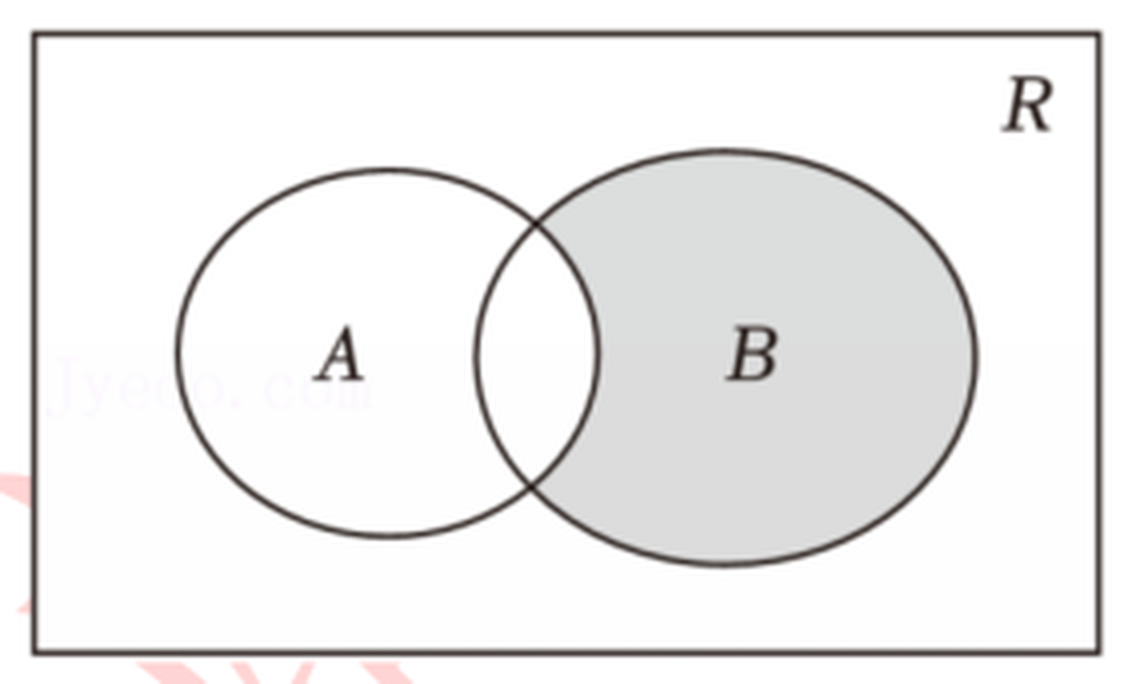
\includegraphics[width=0.30\textwidth]{figures/venn_Abar_cap_B.png}
\end{center}

\begin{enumerate}[label=(\arabic*)]
\item 若 $a=1$，求阴影部分表示的集合.
\item 若 $A\cap B=B$，求实数 $a$ 的取值范围.
\end{enumerate}

\ifanswer
\solbegin
\stepm{(1)}{因为 $\dfrac{2x-3}{x+5}\leqslant0$，
等价于 $\begin{cases}(2x-3)(x+5)\leqslant0\\ x+5\neq0\end{cases}$，}
\step{解得 $-5<x\leqslant\dfrac32$，即 $A=\left\{x\mid-5<x\leqslant\dfrac32\right\}$；}
\step{若 $a=1$，因为 $|x-1|<1$，等价于 $-1<x-1<1$，}
\step{解得 $0<x<2$，即 $B=\{x\mid0<x<2\}$.}
\step{由 Venn 图得阴影部分表示的集合为 $\overline{A}\cap B=\left(\dfrac32,2\right)$.}
\stepm{(2)}{由 (1) 得 $A=\left\{x\mid-5<x\leqslant\dfrac32\right\}$，}
\step{$B=\{x\mid|x-a|<1\}=\{x\mid-1+a<x<1+a\}\neq\varnothing$，}
\step{因为 $A\cap B=B$，所以 $B\sub A$，}
\step{所以 $\begin{cases}-5\leqslant-1+a\\ 1+a\leqslant\dfrac32\end{cases}$，
解得 $-4\leqslant a\leqslant\dfrac12$，}
\step{所以实数 $a$ 的取值范围为 $\left[-4,\dfrac12\right]$.}
\solend

\fi

\ansspace[6]

\item 设 $A=\{x\mid x^2-(m+3)x+2(m+1)=0,m\in\R\}$，
$B=\{x\mid 2x^2+(3n+1)x+2=0,n\in\R\}$.

\begin{enumerate}[label=(\arabic*)]
\item 是否存在 $m$、$n\in\R$，使得 $A=\{1,2\}$，$B=\varnothing$，说明理由；
\item 若 $A\cap B=A$，求 $m$、$n$ 的值.
\end{enumerate}

\ifanswer
\solbegin
\stepm{(1)}{由 $A=\{1,2\}$，得 $m=0$，}
\step{再由 $B=\varnothing$，得 $\Delta=(3n+1)^2-4\times2\times2=9n^2+6n-15<0$，}
\step{所以 $(3n+5)(n-1)<0$，解得 $-\dfrac53<n<1$，}
\step{故存在 $m=0$，$-\dfrac53<n<1$，使得 $A=\{1,2\}$，$B=\varnothing$.}
\stepm{(2)}{由 $x^2-(m+3)x+2(m+1)=0$，得 $x=2$ 或 $x=m+1$，}
\step{若 $A\cap B=A$，则 $A\sub B$，}
\step{将 $x=2$ 代入 $2x^2+(3n+1)x+2=0$，得 $n=-2$，}
\step{则 $B=\{x\mid 2x^2+(3n+1)x+2=0,n\in\R\}=\{x\mid 2x^2-5x+2=0\}
=\left\{2,\dfrac12\right\}$.}
\step{则 $m+1=\dfrac12$ 或 $m+1=2$，则 $m=-\dfrac12$ 或 $m=1$，
所以 $m=-\dfrac12$ 或 $m=1$，$n=-2$.}
\solend

\fi

\ansspace[6]

\item 已知陈述句 $\alpha$：关于 $x$ 的方程 $x^2-6x+m=0$ 有两个不同的正数根，陈述句
$\beta$：集合 $\{x\mid(m+1)x^2+4x+1=0,x\in\R\}$ 中至多有一个元素.

\begin{enumerate}[label=(\arabic*)]
\item 若 $\alpha$ 和 $\beta$ 都是真命题，求实数 $m$ 的取值范围；
\item 若 $\alpha$ 和 $\beta$ 至多有一个是假命题，求实数 $m$ 的取值范围.
\end{enumerate}

\ifanswer
\solbegin
\stepm{(1)}{因为关于 $x$ 的方程 $x^2-6x+m=0$ 有两个不同的正数根，}
\step{则 $\begin{cases}36-4m>0\\ m>0\end{cases}$，解得 $0<m<9$，}
\step{集合 $\{x\mid(m+1)x^2+4x+1=0,x\in\R\}$ 中至多有一个元素，}
\step{则 $m=-1$ 或 $\begin{cases}m+1\neq0\\ 16-4(m+1)\leqslant0\end{cases}$，
解得 $m\geqslant3$，}
\step{$\alpha$ 和 $\beta$ 都是真命题，所以实数 $m$ 的取值范围为 $\{m\mid3\leqslant m<9\}$}
\stepm{(2)}{由 (1) 得当 $\alpha$ 为假命题时，$m\leqslant0$ 或 $m\geqslant9$，}
\step{当 $\beta$ 为假命题时，$m<3$ 且 $m\neq-1$，}
\step{所以 $\alpha$ 和 $\beta$ 均为假命题时，$m$ 的范围是 $m\leqslant0$ 且 $m\neq-1$，}
\step{$\alpha$ 和 $\beta$ 至多有一个是假命题时，实数 $m$ 的取值范围为
$\{m\mid m>0$ 或 $m=-1\}$.}
\solend

\fi

\ansspace[6]

\item 已知符号 $[x]$ 表示不大于 $x$ 的最大整数 $(x\in\R)$，例如：$[1.3]=1$，
$[2]=2$，$[-1.2]=-2$.

\begin{enumerate}[label=(\arabic*)]
\item 已知方程 $[x]=3$，求该方程的解集；
\item 设方程 $\bigl[|x|+|x-1|\bigr]=3$ 的解集为 $A$，
集合 $B=\{x\mid 2x^2-11kx+15k^2\geqslant0\}$，若 $A\cup B=\R$，求实数 $k$ 的取值范围；
\item 在 (2) 的条件下，集合 $C=\{x\mid x^2-ax+1-2a\leqslant0,a\in\R\}$，是否存在实数
$a$，$A\cap C=A$，若存在，请求出实数 $a$ 的取值范围；若不存在，请说明理由.
\end{enumerate}

\ifanswer
\solbegin
\stepm{(1)}{方程 $[x]=3$，则 $x\in[3,4)$，所以该方程的解集为 $[3,4)$；}
\stepm{(2)}{因为 $\bigl[|x|+|x-1|\bigr]=3$，所以 $3\leqslant|x|+|x-1|<4$，}
\step{由绝对值不等式的几何意义得 $A=\left(-\dfrac32,-1\right]\cup\left[2,\dfrac52\right)$，}
\step{又 $B=\{x\mid 2x^2-11kx+15k^2\geqslant0\}=\{x\mid(2x-5k)(x-k)\geqslant0\}$，}
\step{当 $k=0$ 时，$B=\{x\mid 2x^2\geqslant0\}=\R$，则 $A\cup B=\R$，符合题意；}
\step{当 $k>0$ 时，$B=\left(-\infty,\dfrac{5k}{2}\right]\cup[3k,+\infty)$，
若 $A\cup B=\R$，}
\step{则 $\begin{cases}\dfrac{5k}{2}\geqslant2\\[2pt] 3k\leqslant\dfrac52\end{cases}$，
解得 $k\in\left[\dfrac45,\dfrac56\right]$；}
\step{当 $k<0$ 时，$B=(-\infty,3k]\cup\left[\dfrac{5k}{2},+\infty\right)$，
若 $A\cup B=\R$，}
\step{则 $\begin{cases}\dfrac{5k}{2}\leqslant-1\\[2pt] 3k\geqslant-\dfrac32\end{cases}$，
解得 $k\in\left[-\dfrac12,-\dfrac25\right]$.}
\step{综上所述，实数 $k$ 的取值范围为
$\left[-\dfrac12,-\dfrac25\right]\cup\{0\}\cup\left[\dfrac45,\dfrac56\right]$；}
\stepm{(3)}{因为 $A\cap C=A$，则 $A\sub C$ 且
$A=\left(-\dfrac32,-1\right]\cup\left[2,\dfrac52\right)$，}
\step{设集合 $C$ 的解集为 $(x_1,x_2)(x_1<x_2)$，}
\step{则 $\begin{cases}x_1\leqslant-\dfrac32\\[2pt] x_2\geqslant\dfrac52\end{cases}$，}
\step{所以
$\begin{cases}\Delta=a^2-4(1-2a)>0\\[2pt]
f\!\left(-\dfrac32\right)=\dfrac94+\dfrac32a+1-2a\leqslant0\\[4pt]
f\!\left(\dfrac52\right)=\dfrac{25}{4}-\dfrac52a+1-2a\leqslant0\end{cases}$，
解得 $a\geqslant\dfrac{13}{2}$，}
\step{故实数 $a$ 的取值范围为 $\left[\dfrac{13}{2},+\infty\right)$.}
\solend

\fi

\ansspace[6]

\item 非空有限集合 $S$ 是由若干个正实数组成，集合 $S$ 的元素个数不少于 $2$ 个. 对于任意
$a,b\in S,a\neq b$，若数 $a^b$ 或 $b^a$ 中至少有一个属于 $S$，则称集合 $S$ 是“好集”；
否则，称集合 $S$ 是“坏集”.

\begin{enumerate}[label=(\arabic*)]
\item 判断 $A=\{1,3,9\}$ 和 $B=\left\{1,\dfrac12,\dfrac14,\dfrac1{16}\right\}$ 是“好集”
还是“坏集”，并简单说明理由；
\item 题设的有限集 $S$ 中，既有大于 $1$ 的元素，又有小于 $1$ 的元素，证明：集合 $S$ 是
“坏集”；
\item 若题设中的 $a^b$ 或 $b^a$ 都属于 $S$，则称集合 $S$ 为“超级好集”，写出一个
“超级好集”（无须证明）.
\end{enumerate}

\ifanswer
\solbegin
\stepm{(1)}{$A=\{1,3,9\}$，$3^9\notin A$，$9^3\notin A$，所以 $A$ 是“坏集”，}
\step{从 $B$ 集合中任意取两个数字都满足需求，所以 $B$ 是“好集”.}
\stepm{(2)}{假设 $a$ 是 $S$ 中小于 $1$ 的元素中的最小元素，}
\step{$b$ 是 $S$ 中大于 $1$ 的元素中的最小元素，则 $a^b<a^1=a$，}
\step{所以 $a$ 就不是 $S$ 中小于 $1$ 的元素中的最小元素，即 $a^b\notin S$，}
\step{同理 $1=b^0<b^a<b^1=b$，所以 $b$ 就不是 $S$ 中大于 $1$ 的元素中的最小元素，}
\step{即 $b^a\notin S$，所以集合 $S$ 是“坏集”；}
\stepm{(3)}{首先 $S=\{1,a\}$（$a\neq1$ 且 $a>0$）是“超级好集”，}
\step{假设 $0<a<1$，由 (2) 得，$S$ 中不可能有大于 $1$ 的元素，}
\step{假设 $S$ 中有除 $a$ 之外的元素 $b\in S$（$a\neq b,b<1$），}
\step{假设 $a$ 是 $S$ 中小于 $1$ 的元素中的最大元素，$a^b>a^1=a$，}
\step{所以 $a$ 不是最大元素，所以 $a^b\notin S$，所以 $b\notin S$；}
\step{假设 $a>1$，由 (2) 得 $S$ 中不可能有小于 $1$ 的元素，}
\step{假设 $S$ 中有除 $a$ 之外的元素 $b$（$b>1$ 且 $b\neq a$），}
\step{假设 $a$ 是 $S$ 中大于 $1$ 的元素中的最小元素，则 $a^b>a^1=a$，}
\step{所以 $a$ 不是最小元素，即不存在 $b>1$，使得 $b\in S$，即 $b\notin S$，}
\step{综上，$S=\{1,a\}$（$a\neq1$ 且 $a>0$）.}
\solend

\fi

\ansspace*[10]

\end{enumerate}

\end{document}
"
%
% 原始材料是微信公众号图文（公众号「魔都数学加油站」连载「27学年高一 25」，2026-09-21 发布，
% 原文标题「27学年高一25——2026-2027年上海市华师大二附中高一上周末作业3」），
% 正文为 10 张 PNG 页（1080×1527，各页同尺寸）。原文本身就是一份**讲评版**——
% 题目下方直接印出【解析】（本卷无单独的【答案】行，填空题答案都写在解析里）。
% 试题文字与解析均照原卷录入，未改内容。卷面的粉色斜水印「魔都数学加油站」属水印，未录入。
%
% 卷首标题：原卷印作「2026-2027 年华师大二附中高一上周末作业 3」（公众号标题里的「上海市」
% 三字卷面标题行没有，本稿照卷面），年份区间按全稿惯例排 en dash，前缀照原卷保留「年」。
%
% 与原卷的排版差异（均已在 README「说明」中交代）：
%   ① 原文自**第 3 题**起（第 1、2 题未在该文中发布），故本稿题号亦自 3 起；
%   ② 原卷本就印有「一、填空题」「二、选择题」「三、解答题」三节标题，本稿照原卷分节，
%      只把标题改排成全稿统一的「大节标题」样式；
%   ③ 原卷第 13 题的答案「D」直接印在题干末尾的括号内，第 14—16 题的括号空着、答案写在
%      解析末句「故选 C／B」里；填空题的答案也都嵌在解析里，本稿统一改为试卷版隐去、
%      答案版以 \ans{} 给出（选择题另附【解析】），使两版彻底分离；
%   ④ 补集符号原卷一律作**上横线**（$\overline{A}$、$\overline{A\cup B}$），与同校的
%      高一14 同例，本稿照录（不改为 $\complement_U A$ 写法）；
%   ⑤ 原卷的实数集 R 斜体与粗体混用（第 17 题题干「全集为 R」作粗体，第 5、14 题与
%      第 16 题解析的 $R$ 为斜体），本稿按全稿惯例统一写作 $\R$；
%   ⑥ 原卷填空的横线约两个字宽，本稿按全稿惯例统一排 \blankline[4.4em]；
%   ⑦ 原卷未印副标题，本稿按全稿惯例补出副标题「集合与常用逻辑用语」；
%   ⑧ 第 17 题的 Venn 图原卷印在题干右侧（第 6 页），本稿移至题干之后；
%      图取原卷截图、4× LANCZOS 放大（figures/venn_Abar_cap_B.png，
%      阴影为 $B$ 中不含 $A\cap B$ 的部分，即 $\overline{A}\cap B$）。
%
% 原卷存疑两处（均照抄原卷、未改，见源码中该处上方注释）：
%   ① 第 8 题【解析】第二段「当 $\Delta=a^2-16>0$ 时，方程 $x^2+ax+4=0$ 有两个相同的根
%      $x_1$、$x_2$」——$\Delta>0$ 应为「两个**不**相同的根」（其自己的后文就把 $x_1$、$x_2$
%      当作可以不同的两个根在讨论），显系笔误；
%   ② 第 11 题【解析】先写「偶数必是 $2^{11}\cdot3^m\cdot337^n$，$m$、$n\in\N^*$」，
%      下一行又写「$0\leqslant m\leqslant10$，$0\leqslant n\leqslant10$，共有 121 种情况」
%      ——按 $\N^*$ 应从 1 起（至多 $10\times10=100$ 种），与 121（$=11\times11$，含 0）
%      对不上，两处至少有一处笔误。

\documentclass[a4paper,11pt]{article}
\usepackage{common}

\begin{document}

\examtitlest[3]{2026--2027 年华师大二附中高一上周末作业 3}{集合与常用逻辑用语}

\bigsec{一、填空题}

\begin{enumerate}
\setcounter{enumi}{2}

\item 设全集 $U=\{2,4,m^2+m-5\}$，集合 $A=\{2,1-m\}$，若 $\overline{A}=\{1\}$，则实数
$m=$ \blankline[4.4em].

\ifanswer
\solbegin
\step{因为 $\overline{A}=\{1\}$，所以 $1\in U$，$1\notin A$，}
\step{所以 $\begin{cases}m^2+m-5=1\\ 1-m\neq1\\ 1-m=4\end{cases}$，解得 $m=-3$.}
\solend

\fi

\item 已知条件 $\alpha$：$m<x\leqslant2m+5$，条件 $\beta$：$0\leqslant x\leqslant1$，
若 $\alpha$ 是 $\beta$ 的必要条件，则实数 $m$ 的取值范围为 \blankline[4.4em].

\ifanswer
\solbegin
\step{若 $\alpha$ 是 $\beta$ 的必要条件，则 $[0,1]\sub(m,2m+5]$，}
\step{所以 $\begin{cases}m<2m+5\\ m<0\\ 2m+5\geqslant1\end{cases}$，}
\step{解得 $-2\leqslant m<0$，故实数 $m$ 的取值范围为 $[-2,0)$.}
\solend

\fi

\item 已知 $\R$ 是全集，集合 $A=\{y\mid y=-x^2+1,x\in\R\}$，集合
$B=\{x\mid x=3+|a|,a\in\R\}$，则 $\overline{A\cup B}=$ \blankline[4.4em].

\ifanswer
\solbegin
\step{$A=\{y\mid y=-x^2+1,x\in\R\}=(-\infty,1]$，}
\step{$B=\{x\mid x=3+|a|,a\in\R\}=[3,+\infty)$，}
\step{所以 $\overline{A\cup B}=(1,3)$.}
\solend

\fi

\item 已知 $a$ 为常数，集合 $A=\{x\mid x^2+x-6=0\}$，集合 $B=\{x\mid ax-2=0\}$，且
$B\sub A$，则 $a$ 的所有取值构成的集合为 \blankline[4.4em].

\ifanswer
\solbegin
\step{集合 $A=\{-3,2\}$，因为 $B\sub A$，所以 $B=\varnothing$，$\{-3\}$，$\{2\}$，$\{-3,2\}$，}
\step{当 $B=\varnothing$ 时，$a=0$，当 $B=\{-3\}$ 时，$a=-\dfrac23$，当 $B=\{2\}$ 时，$a=1$，}
\step{当 $B=\{-3,2\}$ 时，不成立，故 $a$ 的取值集合为 $\left\{0,-\dfrac23,1\right\}$.}
\solend

\fi

\item 已知一元二次方程 $x^2+px+p=0$ 有两个不相等的实根分别为 $x_1$、$x_2$.
$A=x_1^2+x_2^2$，$B=x_1x_2(x_1+x_2)$，$A$ 与 $B$ 的大小为 \blankline[4.4em].

\ifanswer
\solbegin
\step{一元二次方程 $x^2+px+p=0$ 有两个不相等的实根分别为 $x_1$、$x_2$，}
\step{则 $\Delta=p^2-4p>0$，解得 $p<0$ 或 $p>4$，}
\step{由韦达定理得 $x_1+x_2=-p$，$x_1x_2=p$，}
\step{所以 $A=x_1^2+x_2^2=(x_1+x_2)^2-2x_1x_2=p^2-2p$，$B=x_1x_2(x_1+x_2)=-p^2$，}
\step{所以 $A-B=(p^2-2p)-(-p^2)=2p(p-1)$，}
\step{当 $p<0$ 时，则 $A-B>0$，故 $A>B$，}
\step{当 $p>4$ 时，则 $A-B>0$，故 $A>B$，}
\step{综上，$A=p^2-2p$，$B=-p^2$，且 $A>B$.}
\solend

\fi

\item 集合 $A=\{x\mid(x-1)(x^2+ax+4)=0,x\in\R\}$ 中所有元素之和为 $3$，则实数
$a=$ \blankline[4.4em].

\ifanswer
\solbegin
\step{当 $\Delta=a^2-16=0$ 时，方程 $x^2+ax+4=0$ 有两个相同的根 $-\dfrac a2$，}
\step{则 $A=\left\{1,-\dfrac a2\right\}$，故 $1-\dfrac a2=3$，解得 $a=-4$；}
% 注：下一行的「两个相同的根」系原卷笔误（△>0 应为「两个不相同的根」，其自己的后文
%     就把 x₁、x₂ 当作可以不同的两个根在讨论），照抄原卷、未改，见文件头「原卷存疑」①。
\step{当 $\Delta=a^2-16>0$ 时，方程 $x^2+ax+4=0$ 有两个相同的根 $x_1$、$x_2$，}
\step{若 $1$ 是方程 $x^2+ax+4=0$ 的根，则方程 $x^2+ax+4=0$ 的另一个根为 $4$，}
\step{则 $A=\{1,4\}$，不成立；}
\step{若 $1$ 不是方程 $x^2+ax+4=0$ 的根，则 $A=\{1,x_1,x_2\}$，则 $1+x_1+x_2=3$，}
\step{故 $x_1+x_2=2=-a$，故 $a=-2$（舍去）；}
\step{综上所述，$a=-4$.}
\solend

\fi

\item 已知集合 $A=\{x\mid x^2+2x-8\geqslant0\}$，$B=\{x\mid x^2-2ax+4\leqslant0\}$，
若 $a>0$，且 $A\cap B\cap\N$ 中恰有 $2$ 个元素，则 $a$ 的取值范围为 \blankline[4.4em].

\ifanswer
\solbegin
\step{由 $A$ 中不等式变形得 $(x-2)(x+4)\geqslant0$，解得 $x\leqslant-4$ 或 $x\geqslant2$，}
\step{即 $A=(-\infty,-4]\cup[2,+\infty)$，}
\step{设 $f(x)=x^2-2ax+4$，则 $f(x)$ 的轴对称 $x=a>0$，}
\step{且对应方程的根 $x_1$、$x_2$ 满足 $\begin{cases}x_1x_2=4\\ x_1+x_2>0\end{cases}$，}
\step{所以 $0<x_1\leqslant2\leqslant x_2$（取 $x_1\leqslant x_2$），}
\step{所以 $A\cap B\cap\N$ 中恰有的整数为 $2$，$3$，}
\step{所以 $\begin{cases}f(3)=9-6a+4\leqslant0\\ f(4)=16-8a+4>0\end{cases}$，}
\step{解得 $\dfrac{13}{6}\leqslant a<\dfrac52$，所以 $a$ 的取值范围为 $\left[\dfrac{13}{6},\dfrac52\right)$.}
\solend

\fi

\item 在三个关于 $x$ 的方程 $x^2-ax+4=0$，$x^2+(a-1)x+16=0$ 和
$x^2+2ax+3a+10=0$ 中至少有一个方程有实根，则实数 $a$ 的取值范围是 \blankline[4.4em].

\ifanswer
\solbegin
\step{当三个方程均无实根时，有}
\step{$\begin{cases}\Delta_1=a^2-16<0\\ \Delta_2=(a-1)^2-64<0\\ \Delta_3=4a^2-4(3a+10)<0\end{cases}$，}
\step{所以 $\begin{cases}-4<a<4\\ -7<a<9\\ -2<a<5\end{cases}$，}
\step{所以 $-2<a<4$，故三个方程均无实根时，$a$ 的取值范围为 $(-2,4)$，}
\step{所以三个方程中至少有一个方程有实根时，}
\step{实数 $a$ 的取值范围为 $(-\infty,-2]\cup[4,+\infty)$.}
\solend

\fi

% 注：下一行解析里的「m、n∈N*」与再下一行的「0≤m≤10，0≤n≤10，共有 121 种情况」
%     对不上（按 N* 应从 1 起，至多 10×10=100 种；121=11×11 含 0），系原卷自身矛盾，
%     照抄原卷、未改，见文件头「原卷存疑」②。
\item 若集合 $M=\{(x,y)\mid(x+1)+(x+2)+\cdots+(x+y)=2022^{10},x\in\Z,y\in\N^{*}\}$，
则集合 $M$ 中元素有 \blankline[4.4em] 个.

\ifanswer
\solbegin
\step{由题意得 $(x+1)+(x+2)+\cdots+(x+y)=\dfrac{y(2x+1+y)}{2}$，}
\step{所以 $y(2x+1+y)=2^{11}\cdot3^{10}\cdot337^{10}$，}
\step{因为 $y$ 与 $2x+1+y$ 必为一奇一偶，偶数必是 $2^{11}\cdot3^m\cdot337^n$，
$m$、$n\in\N^{*}$，}
\step{$0\leqslant m\leqslant10$，$0\leqslant n\leqslant10$，共有 $121$ 种情况，}
\step{因为 $y$ 与 $2x+1+y$ 奇偶未定，所以集合 $M$ 中元素只有 $242$ 个.}
\solend

\fi

\item 设集合 $M=\left\{x\mid m\leqslant x\leqslant m+\dfrac34\right\}$，
$N=\left\{x\mid n-\dfrac13\leqslant x\leqslant n\right\}$，且 $M$、$N$ 都是集合
$\{x\mid0\leqslant x\leqslant1\}$ 的子集，如果把 $b-a$ 叫做集合
$\{x\mid a\leqslant x\leqslant b\}$ 的长度，那么集合 $M\cap N$ 的长度的最小值是
\blankline[4.4em].

\ifanswer
\solbegin
\step{$M$ 的长度为 $\dfrac34$，$N$ 的长度为 $\dfrac13$，}
\step{当集合 $M\cap N$ 的长度的最小值时，$M$ 与 $N$ 应分别在区间 $[0,1]$ 的左右两端，}
\step{故 $M\cap N$ 的长度的最小值是 $\dfrac34+\dfrac13-1=\dfrac1{12}$.}
\solend

\fi

\end{enumerate}

\bigsec{二、选择题}

\begin{enumerate}
\setcounter{enumi}{12}

\item 直角坐标平面中除去两点 $A(1,1)$、$B(2,-2)$ 可用集合表示为\mbox{（\quad）}

\keepwithprev
A. $\{(x,y)\mid x\neq1,y\neq1,x\neq2,y\neq-2$\}\qquad
B. $\{(x,y)\mid\begin{cases}x\neq1\\ y\neq1\end{cases}$ 或 $\begin{cases}x\neq2\\ y\neq-2\end{cases}\}$

C. $\{(x,y)\mid[(x-1)^2+(y-1)^2][(x-2)^2+(y+2)^2]\neq0$\}

D. $\{(x,y)\mid[(x-1)^2+(y-1)^2]+[(x-2)^2+(y+2)^2]\neq0$\}

\ans{$D$}

\item 已知函数 $f(x)=x^2+nx$，记集合 $A=\{x\mid f(x)=0,x\in\R\}$，
$B=\{x\mid f(f(x))=0,x\in\R\}$，若 $A=B\neq\varnothing$，则 $n$ 的取值范围是\mbox{（\quad）}

\keepwithprev
A. $[0,4]$\qquad B. $(0,4)$\qquad C. $[0,4)$\qquad D. $(0,4]$

\ans{$C$}

\ifanswer
\solbegin
\step{$f(x)=x^2+nx$，$f[f(x)]=(x^2+nx)^2+n(x^2+nx)=(x^2+nx)(x^2+nx+n)$，}
\step{当 $n=0$ 时，$f(x)=x^2$，$f[f(x)]=x^4$，满足 $A=B$，此时 $n=0$；}
\step{当 $n\neq0$ 时，$0$、$-n$ 不是 $x^2+nx+n=0$ 的根，故 $\Delta=n^2-4n<0$，
解得 $0<n<4$，}
\step{综上所述，$n$ 的取值范围是 $[0,4)$. 故选 $C$.}
\solend

\fi

\item 设全集 $U=\{1,2,3,4,5,6,7,8,9,10\}$，给出条件：① $A\sub U$；②若 $x\in A$，
则 $2x\notin A$；③若 $x\in\overline{A}$，则 $2x\notin\overline{A}$.
那么同时满足三个条件的集合 $A$ 的个数为\mbox{（\quad）}

\keepwithprev
A. $0$ 个\qquad B. $16$ 个\qquad C. $32$ 个\qquad D. $64$ 个

\ans{$C$}

\ifanswer
\solbegin
\step{由① $A\sub U$；②若 $x\in A$，则 $2x\notin A$；③若 $x\in\overline{A}$，
则 $2x\notin\overline{A}$.}
\step{若 $1\in A$，则 $2\notin A$，即 $2\in\overline{A}$，则 $4\notin\overline{A}$，
即 $4\in A$，则 $8\notin A$，即 $8\in\overline{A}$；}
\step{若 $3\in A$，则 $6\notin A$，即 $6\in\overline{A}$；若 $5\in A$，则 $10\notin A$，
即 $10\in\overline{A}$，}
\step{故 $1$、$4$ 和 $2$、$8$ 分开，$3$ 和 $6$ 分开，$5$ 和 $10$ 分开，$7$ 和 $9$ 随意，}
\step{故同时满足三个条件的集合 $A$ 的个数为 $2\times2\times2\times2\times2=32$，
故选 $C$.}
\solend

\fi

\item 设集合 $P_1=\{x\mid x^2+ax+1>0\}$，$P_2=\{x\mid x^2+ax+2>0\}$，
$Q_1=\{x\mid x^2+x+b>0\}$，$Q_2=\{x\mid x^2+2x+b>0\}$，其中 $a$、$b\in\R$，
下列说法中正确的是\mbox{（\quad）}

\keepwithprev
A. 对任意 $a$，$P_1$ 是 $P_2$ 的子集，对任意的 $b$，$Q_1$ 不是 $Q_2$ 的子集

B. 对任意 $a$，$P_1$ 是 $P_2$ 的子集，存在 $b$，使得 $Q_1$ 是 $Q_2$ 的子集

C. 存在 $a$，使得 $P_1$ 不是 $P_2$ 的子集，对任意的 $b$，$Q_1$ 不是 $Q_2$ 的子集

D. 存在 $a$，使得 $P_1$ 不是 $P_2$ 的子集，存在 $b$，使得 $Q_1$ 是 $Q_2$ 的子集

\ans{$B$}

\ifanswer
\solbegin
\step{对于集合 $P_1=\{x\mid x^2+ax+1>0\}$，$P_2=\{x\mid x^2+ax+2>0\}$，}
\step{得当 $m\in P_1$ 时，即 $m^2+am+1>0$，得 $m^2+am+2>0$，}
\step{即有 $m\in P_2$，得对任意 $a$，$P_1$ 是 $P_2$ 的子集，}
\step{对于集合 $Q_1=\{x\mid x^2+x+b>0\}$，$Q_2=\{x\mid x^2+2x+b>0\}$，}
\step{当 $b=6$ 时，$Q_1=\{x\mid x^2+x+6>0\}=\R$，$Q_2=\{x\mid x^2+2x+6>0\}=\R$，}
\step{得 $Q_1$ 是 $Q_2$ 的子集，}
\step{当 $b=1$ 时，$Q_1=\{x\mid x^2+x+1>0\}=\R$，}
\step{$Q_2=\{x\mid x^2+2x+1>0\}=\{x\mid x\neq-1\}$，得 $Q_1$ 不是 $Q_2$ 的子集，}
\step{所以存在 $b$，使得 $Q_1$ 是 $Q_2$ 的子集，故选 $B$.}
\solend

\fi

\end{enumerate}

\bigsec{三、解答题}

\begin{enumerate}
\setcounter{enumi}{16}

\item 已知集合 $A=\left\{x\mid\dfrac{2x-3}{x+5}\leqslant0\right\}$，
$B=\{x\mid|x-a|<1\}$，全集为 $\R$.

\begin{center}
% 图取原卷截图、4× LANCZOS 放大（原卷把图印在题干右侧，本稿移至此处，见文件头⑧）。
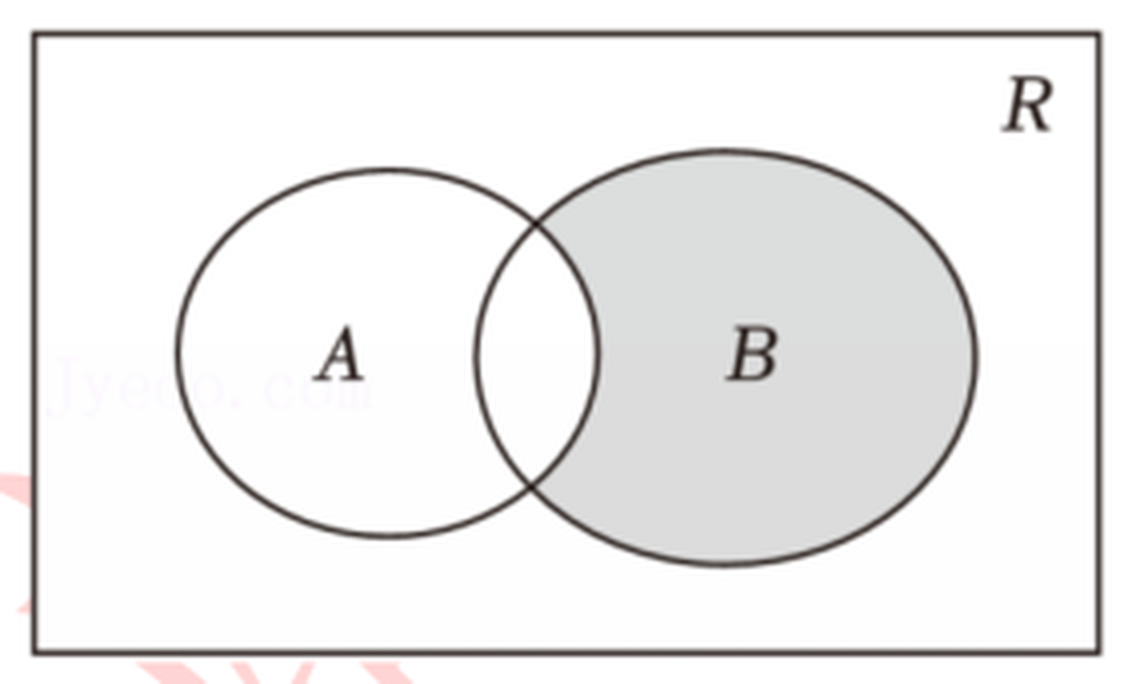
\includegraphics[width=0.30\textwidth]{figures/venn_Abar_cap_B.png}
\end{center}

\begin{enumerate}[label=(\arabic*)]
\item 若 $a=1$，求阴影部分表示的集合.
\item 若 $A\cap B=B$，求实数 $a$ 的取值范围.
\end{enumerate}

\ifanswer
\solbegin
\stepm{(1)}{因为 $\dfrac{2x-3}{x+5}\leqslant0$，
等价于 $\begin{cases}(2x-3)(x+5)\leqslant0\\ x+5\neq0\end{cases}$，}
\step{解得 $-5<x\leqslant\dfrac32$，即 $A=\left\{x\mid-5<x\leqslant\dfrac32\right\}$；}
\step{若 $a=1$，因为 $|x-1|<1$，等价于 $-1<x-1<1$，}
\step{解得 $0<x<2$，即 $B=\{x\mid0<x<2\}$.}
\step{由 Venn 图得阴影部分表示的集合为 $\overline{A}\cap B=\left(\dfrac32,2\right)$.}
\stepm{(2)}{由 (1) 得 $A=\left\{x\mid-5<x\leqslant\dfrac32\right\}$，}
\step{$B=\{x\mid|x-a|<1\}=\{x\mid-1+a<x<1+a\}\neq\varnothing$，}
\step{因为 $A\cap B=B$，所以 $B\sub A$，}
\step{所以 $\begin{cases}-5\leqslant-1+a\\ 1+a\leqslant\dfrac32\end{cases}$，
解得 $-4\leqslant a\leqslant\dfrac12$，}
\step{所以实数 $a$ 的取值范围为 $\left[-4,\dfrac12\right]$.}
\solend

\fi

\ansspace[6]

\item 设 $A=\{x\mid x^2-(m+3)x+2(m+1)=0,m\in\R\}$，
$B=\{x\mid 2x^2+(3n+1)x+2=0,n\in\R\}$.

\begin{enumerate}[label=(\arabic*)]
\item 是否存在 $m$、$n\in\R$，使得 $A=\{1,2\}$，$B=\varnothing$，说明理由；
\item 若 $A\cap B=A$，求 $m$、$n$ 的值.
\end{enumerate}

\ifanswer
\solbegin
\stepm{(1)}{由 $A=\{1,2\}$，得 $m=0$，}
\step{再由 $B=\varnothing$，得 $\Delta=(3n+1)^2-4\times2\times2=9n^2+6n-15<0$，}
\step{所以 $(3n+5)(n-1)<0$，解得 $-\dfrac53<n<1$，}
\step{故存在 $m=0$，$-\dfrac53<n<1$，使得 $A=\{1,2\}$，$B=\varnothing$.}
\stepm{(2)}{由 $x^2-(m+3)x+2(m+1)=0$，得 $x=2$ 或 $x=m+1$，}
\step{若 $A\cap B=A$，则 $A\sub B$，}
\step{将 $x=2$ 代入 $2x^2+(3n+1)x+2=0$，得 $n=-2$，}
\step{则 $B=\{x\mid 2x^2+(3n+1)x+2=0,n\in\R\}=\{x\mid 2x^2-5x+2=0\}
=\left\{2,\dfrac12\right\}$.}
\step{则 $m+1=\dfrac12$ 或 $m+1=2$，则 $m=-\dfrac12$ 或 $m=1$，
所以 $m=-\dfrac12$ 或 $m=1$，$n=-2$.}
\solend

\fi

\ansspace[6]

\item 已知陈述句 $\alpha$：关于 $x$ 的方程 $x^2-6x+m=0$ 有两个不同的正数根，陈述句
$\beta$：集合 $\{x\mid(m+1)x^2+4x+1=0,x\in\R\}$ 中至多有一个元素.

\begin{enumerate}[label=(\arabic*)]
\item 若 $\alpha$ 和 $\beta$ 都是真命题，求实数 $m$ 的取值范围；
\item 若 $\alpha$ 和 $\beta$ 至多有一个是假命题，求实数 $m$ 的取值范围.
\end{enumerate}

\ifanswer
\solbegin
\stepm{(1)}{因为关于 $x$ 的方程 $x^2-6x+m=0$ 有两个不同的正数根，}
\step{则 $\begin{cases}36-4m>0\\ m>0\end{cases}$，解得 $0<m<9$，}
\step{集合 $\{x\mid(m+1)x^2+4x+1=0,x\in\R\}$ 中至多有一个元素，}
\step{则 $m=-1$ 或 $\begin{cases}m+1\neq0\\ 16-4(m+1)\leqslant0\end{cases}$，
解得 $m\geqslant3$，}
\step{$\alpha$ 和 $\beta$ 都是真命题，所以实数 $m$ 的取值范围为 $\{m\mid3\leqslant m<9\}$}
\stepm{(2)}{由 (1) 得当 $\alpha$ 为假命题时，$m\leqslant0$ 或 $m\geqslant9$，}
\step{当 $\beta$ 为假命题时，$m<3$ 且 $m\neq-1$，}
\step{所以 $\alpha$ 和 $\beta$ 均为假命题时，$m$ 的范围是 $m\leqslant0$ 且 $m\neq-1$，}
\step{$\alpha$ 和 $\beta$ 至多有一个是假命题时，实数 $m$ 的取值范围为
$\{m\mid m>0$ 或 $m=-1\}$.}
\solend

\fi

\ansspace[6]

\item 已知符号 $[x]$ 表示不大于 $x$ 的最大整数 $(x\in\R)$，例如：$[1.3]=1$，
$[2]=2$，$[-1.2]=-2$.

\begin{enumerate}[label=(\arabic*)]
\item 已知方程 $[x]=3$，求该方程的解集；
\item 设方程 $\bigl[|x|+|x-1|\bigr]=3$ 的解集为 $A$，
集合 $B=\{x\mid 2x^2-11kx+15k^2\geqslant0\}$，若 $A\cup B=\R$，求实数 $k$ 的取值范围；
\item 在 (2) 的条件下，集合 $C=\{x\mid x^2-ax+1-2a\leqslant0,a\in\R\}$，是否存在实数
$a$，$A\cap C=A$，若存在，请求出实数 $a$ 的取值范围；若不存在，请说明理由.
\end{enumerate}

\ifanswer
\solbegin
\stepm{(1)}{方程 $[x]=3$，则 $x\in[3,4)$，所以该方程的解集为 $[3,4)$；}
\stepm{(2)}{因为 $\bigl[|x|+|x-1|\bigr]=3$，所以 $3\leqslant|x|+|x-1|<4$，}
\step{由绝对值不等式的几何意义得 $A=\left(-\dfrac32,-1\right]\cup\left[2,\dfrac52\right)$，}
\step{又 $B=\{x\mid 2x^2-11kx+15k^2\geqslant0\}=\{x\mid(2x-5k)(x-k)\geqslant0\}$，}
\step{当 $k=0$ 时，$B=\{x\mid 2x^2\geqslant0\}=\R$，则 $A\cup B=\R$，符合题意；}
\step{当 $k>0$ 时，$B=\left(-\infty,\dfrac{5k}{2}\right]\cup[3k,+\infty)$，
若 $A\cup B=\R$，}
\step{则 $\begin{cases}\dfrac{5k}{2}\geqslant2\\[2pt] 3k\leqslant\dfrac52\end{cases}$，
解得 $k\in\left[\dfrac45,\dfrac56\right]$；}
\step{当 $k<0$ 时，$B=(-\infty,3k]\cup\left[\dfrac{5k}{2},+\infty\right)$，
若 $A\cup B=\R$，}
\step{则 $\begin{cases}\dfrac{5k}{2}\leqslant-1\\[2pt] 3k\geqslant-\dfrac32\end{cases}$，
解得 $k\in\left[-\dfrac12,-\dfrac25\right]$.}
\step{综上所述，实数 $k$ 的取值范围为
$\left[-\dfrac12,-\dfrac25\right]\cup\{0\}\cup\left[\dfrac45,\dfrac56\right]$；}
\stepm{(3)}{因为 $A\cap C=A$，则 $A\sub C$ 且
$A=\left(-\dfrac32,-1\right]\cup\left[2,\dfrac52\right)$，}
\step{设集合 $C$ 的解集为 $(x_1,x_2)(x_1<x_2)$，}
\step{则 $\begin{cases}x_1\leqslant-\dfrac32\\[2pt] x_2\geqslant\dfrac52\end{cases}$，}
\step{所以
$\begin{cases}\Delta=a^2-4(1-2a)>0\\[2pt]
f\!\left(-\dfrac32\right)=\dfrac94+\dfrac32a+1-2a\leqslant0\\[4pt]
f\!\left(\dfrac52\right)=\dfrac{25}{4}-\dfrac52a+1-2a\leqslant0\end{cases}$，
解得 $a\geqslant\dfrac{13}{2}$，}
\step{故实数 $a$ 的取值范围为 $\left[\dfrac{13}{2},+\infty\right)$.}
\solend

\fi

\ansspace[6]

\item 非空有限集合 $S$ 是由若干个正实数组成，集合 $S$ 的元素个数不少于 $2$ 个. 对于任意
$a,b\in S,a\neq b$，若数 $a^b$ 或 $b^a$ 中至少有一个属于 $S$，则称集合 $S$ 是“好集”；
否则，称集合 $S$ 是“坏集”.

\begin{enumerate}[label=(\arabic*)]
\item 判断 $A=\{1,3,9\}$ 和 $B=\left\{1,\dfrac12,\dfrac14,\dfrac1{16}\right\}$ 是“好集”
还是“坏集”，并简单说明理由；
\item 题设的有限集 $S$ 中，既有大于 $1$ 的元素，又有小于 $1$ 的元素，证明：集合 $S$ 是
“坏集”；
\item 若题设中的 $a^b$ 或 $b^a$ 都属于 $S$，则称集合 $S$ 为“超级好集”，写出一个
“超级好集”（无须证明）.
\end{enumerate}

\ifanswer
\solbegin
\stepm{(1)}{$A=\{1,3,9\}$，$3^9\notin A$，$9^3\notin A$，所以 $A$ 是“坏集”，}
\step{从 $B$ 集合中任意取两个数字都满足需求，所以 $B$ 是“好集”.}
\stepm{(2)}{假设 $a$ 是 $S$ 中小于 $1$ 的元素中的最小元素，}
\step{$b$ 是 $S$ 中大于 $1$ 的元素中的最小元素，则 $a^b<a^1=a$，}
\step{所以 $a$ 就不是 $S$ 中小于 $1$ 的元素中的最小元素，即 $a^b\notin S$，}
\step{同理 $1=b^0<b^a<b^1=b$，所以 $b$ 就不是 $S$ 中大于 $1$ 的元素中的最小元素，}
\step{即 $b^a\notin S$，所以集合 $S$ 是“坏集”；}
\stepm{(3)}{首先 $S=\{1,a\}$（$a\neq1$ 且 $a>0$）是“超级好集”，}
\step{假设 $0<a<1$，由 (2) 得，$S$ 中不可能有大于 $1$ 的元素，}
\step{假设 $S$ 中有除 $a$ 之外的元素 $b\in S$（$a\neq b,b<1$），}
\step{假设 $a$ 是 $S$ 中小于 $1$ 的元素中的最大元素，$a^b>a^1=a$，}
\step{所以 $a$ 不是最大元素，所以 $a^b\notin S$，所以 $b\notin S$；}
\step{假设 $a>1$，由 (2) 得 $S$ 中不可能有小于 $1$ 的元素，}
\step{假设 $S$ 中有除 $a$ 之外的元素 $b$（$b>1$ 且 $b\neq a$），}
\step{假设 $a$ 是 $S$ 中大于 $1$ 的元素中的最小元素，则 $a^b>a^1=a$，}
\step{所以 $a$ 不是最小元素，即不存在 $b>1$，使得 $b\in S$，即 $b\notin S$，}
\step{综上，$S=\{1,a\}$（$a\neq1$ 且 $a>0$）.}
\solend

\fi

\ansspace*[10]

\end{enumerate}

\end{document}
